\documentclass[twoside]{book}

% Packages required by doxygen
\usepackage{fixltx2e}
\usepackage{calc}
\usepackage{doxygen}
\usepackage[export]{adjustbox} % also loads graphicx
\usepackage{graphicx}
\usepackage[utf8]{inputenc}
\usepackage{makeidx}
\usepackage{multicol}
\usepackage{multirow}
\PassOptionsToPackage{warn}{textcomp}
\usepackage{textcomp}
\usepackage[nointegrals]{wasysym}
\usepackage[table]{xcolor}

% Font selection
\usepackage[T1]{fontenc}
\usepackage[scaled=.90]{helvet}
\usepackage{courier}
\usepackage{amssymb}
\usepackage{sectsty}
\renewcommand{\familydefault}{\sfdefault}
\allsectionsfont{%
  \fontseries{bc}\selectfont%
  \color{darkgray}%
}
\renewcommand{\DoxyLabelFont}{%
  \fontseries{bc}\selectfont%
  \color{darkgray}%
}
\newcommand{\+}{\discretionary{\mbox{\scriptsize$\hookleftarrow$}}{}{}}

% Page & text layout
\usepackage{geometry}
\geometry{%
  a4paper,%
  top=2.5cm,%
  bottom=2.5cm,%
  left=2.5cm,%
  right=2.5cm%
}
\tolerance=750
\hfuzz=15pt
\hbadness=750
\setlength{\emergencystretch}{15pt}
\setlength{\parindent}{0cm}
\setlength{\parskip}{3ex plus 2ex minus 2ex}
\makeatletter
\renewcommand{\paragraph}{%
  \@startsection{paragraph}{4}{0ex}{-1.0ex}{1.0ex}{%
    \normalfont\normalsize\bfseries\SS@parafont%
  }%
}
\renewcommand{\subparagraph}{%
  \@startsection{subparagraph}{5}{0ex}{-1.0ex}{1.0ex}{%
    \normalfont\normalsize\bfseries\SS@subparafont%
  }%
}
\makeatother

% Headers & footers
\usepackage{fancyhdr}
\pagestyle{fancyplain}
\fancyhead[LE]{\fancyplain{}{\bfseries\thepage}}
\fancyhead[CE]{\fancyplain{}{}}
\fancyhead[RE]{\fancyplain{}{\bfseries\leftmark}}
\fancyhead[LO]{\fancyplain{}{\bfseries\rightmark}}
\fancyhead[CO]{\fancyplain{}{}}
\fancyhead[RO]{\fancyplain{}{\bfseries\thepage}}
\fancyfoot[LE]{\fancyplain{}{}}
\fancyfoot[CE]{\fancyplain{}{}}
\fancyfoot[RE]{\fancyplain{}{\bfseries\scriptsize Generated by Doxygen }}
\fancyfoot[LO]{\fancyplain{}{\bfseries\scriptsize Generated by Doxygen }}
\fancyfoot[CO]{\fancyplain{}{}}
\fancyfoot[RO]{\fancyplain{}{}}
\renewcommand{\footrulewidth}{0.4pt}
\renewcommand{\chaptermark}[1]{%
  \markboth{#1}{}%
}
\renewcommand{\sectionmark}[1]{%
  \markright{\thesection\ #1}%
}

% Indices & bibliography
\usepackage{natbib}
\usepackage[titles]{tocloft}
\setcounter{tocdepth}{3}
\setcounter{secnumdepth}{5}
\makeindex

% Hyperlinks (required, but should be loaded last)
\usepackage{ifpdf}
\ifpdf
  \usepackage[pdftex,pagebackref=true]{hyperref}
\else
  \usepackage[ps2pdf,pagebackref=true]{hyperref}
\fi
\hypersetup{%
  colorlinks=true,%
  linkcolor=blue,%
  citecolor=blue,%
  unicode%
}

% Custom commands
\newcommand{\clearemptydoublepage}{%
  \newpage{\pagestyle{empty}\cleardoublepage}%
}

\usepackage{caption}
\captionsetup{labelsep=space,justification=centering,font={bf},singlelinecheck=off,skip=4pt,position=top}

%===== C O N T E N T S =====

\begin{document}

% Titlepage & ToC
\hypersetup{pageanchor=false,
             bookmarksnumbered=true,
             pdfencoding=unicode
            }
\pagenumbering{alph}
\begin{titlepage}
\vspace*{7cm}
\begin{center}%
{\Large R\+F\+I\+M\+S-\/\+C\+A\+RT }\\
\vspace*{1cm}
{\large Generated by Doxygen 1.8.13}\\
\end{center}
\end{titlepage}
\clearemptydoublepage
\pagenumbering{roman}
\tableofcontents
\clearemptydoublepage
\pagenumbering{arabic}
\hypersetup{pageanchor=true}

%--- Begin generated contents ---
\chapter{R\+F\+I\+M\+S\+\_\+\+C\+A\+RT}
\label{md_README}
\Hypertarget{md_README}
This software is intended to run in the \char`\"{}\+R\+F Interference Measurement System (\+R\+F\+I\+M\+S)\char`\"{} which is going to be installed beside the China-\/\+Argentina Radio Telescope (C\+A\+RT) to analize the \hyperlink{structRFI}{R\+FI} which could reach the telescope. The aim of this system is to measure the RF signals which arrive at the place where the telescope will be installed, taking into account different azimuth positions and two antenna polarizations, horizontal and vertical. Then, it must process the sweeps, identify the interferences and register them in a database.

Also, this software must generate the signals to drive the antenna positioning system and capture and process the signals which will be sent by this system in response.

Moreover, this software must do a front end calibration every so often. This process consists in disconnecting the antenna and connecting a noise source to the system input, capturing sweeps with this device turned on and off and then processing these sweeps to get the actual parameters of the front end\+: gain and noise source versus frequency. 
\chapter{Hierarchical Index}
\section{Class Hierarchy}
This inheritance list is sorted roughly, but not completely, alphabetically\+:\begin{DoxyCompactList}
\item \contentsline{section}{Antenna\+Positioner}{\pageref{classAntennaPositioner}}{}
\item \contentsline{section}{Band\+Parameters}{\pageref{structBandParameters}}{}
\item \contentsline{section}{Command}{\pageref{classCommand}}{}
\item \contentsline{section}{Curve\+Adjuster}{\pageref{classCurveAdjuster}}{}
\item \contentsline{section}{Data3D}{\pageref{structData3D}}{}
\item \contentsline{section}{Data\+Logger}{\pageref{classDataLogger}}{}
\item exception\begin{DoxyCompactList}
\item \contentsline{section}{rfims\+\_\+exception}{\pageref{classrfims__exception}}{}
\end{DoxyCompactList}
\item \contentsline{section}{Spectran\+Configurator\+:\+:Fixed\+Parameters}{\pageref{structSpectranConfigurator_1_1FixedParameters}}{}
\item \contentsline{section}{Float\+To\+Bytes}{\pageref{unionFloatToBytes}}{}
\item \contentsline{section}{Freq\+Values}{\pageref{structFreqValues}}{}
\begin{DoxyCompactList}
\item \contentsline{section}{R\+FI}{\pageref{structRFI}}{}
\item \contentsline{section}{Sweep}{\pageref{structSweep}}{}
\end{DoxyCompactList}
\item \contentsline{section}{Front\+End\+Calibrator}{\pageref{classFrontEndCalibrator}}{}
\item \contentsline{section}{G\+P\+S\+Coordinates}{\pageref{structGPSCoordinates}}{}
\item \contentsline{section}{G\+P\+S\+Interface}{\pageref{classGPSInterface}}{}
\item \contentsline{section}{Reply}{\pageref{classReply}}{}
\begin{DoxyCompactList}
\item \contentsline{section}{Sweep\+Reply}{\pageref{classSweepReply}}{}
\end{DoxyCompactList}
\item \contentsline{section}{R\+F\+I\+Detector}{\pageref{classRFIDetector}}{}
\item \contentsline{section}{R\+F\+Plotter}{\pageref{classRFPlotter}}{}
\item \contentsline{section}{Signal\+Handler}{\pageref{classSignalHandler}}{}
\item \contentsline{section}{Spectran\+Configurator}{\pageref{classSpectranConfigurator}}{}
\item \contentsline{section}{Spectran\+Interface}{\pageref{classSpectranInterface}}{}
\item \contentsline{section}{Sweep\+Builder}{\pageref{classSweepBuilder}}{}
\item \contentsline{section}{Time\+Data}{\pageref{structTimeData}}{}
\end{DoxyCompactList}

\chapter{Class Index}
\section{Class List}
Here are the classes, structs, unions and interfaces with brief descriptions\+:\begin{DoxyCompactList}
\item\contentsline{section}{\hyperlink{classAntennaPositioner}{Antenna\+Positioner} \\*The aim of this class is to drive the antenna positioning }{\pageref{classAntennaPositioner}}{}
\item\contentsline{section}{\hyperlink{structBandParameters}{Band\+Parameters} \\*This structure is intended to store the parameters which are used to configure the spectrum analyzer in each frequency band }{\pageref{structBandParameters}}{}
\item\contentsline{section}{\hyperlink{classCommand}{Command} \\*This class builds the corresponding bytes array to send a certain command to a Aaronia Spectran V4 series spectrum analyzer }{\pageref{classCommand}}{}
\item\contentsline{section}{\hyperlink{classCurveAdjuster}{Curve\+Adjuster} }{\pageref{classCurveAdjuster}}{}
\item\contentsline{section}{\hyperlink{classCustomException}{Custom\+Exception} \\*A class derived from standard class {\ttfamily std\+::exception} }{\pageref{classCustomException}}{}
\item\contentsline{section}{\hyperlink{structData3D}{Data3D} \\*A structure intended to save the the tri-\/axial values of the 3D sensors which are integrated in the G\+PS receiver }{\pageref{structData3D}}{}
\item\contentsline{section}{\hyperlink{classDataLogger}{Data\+Logger} }{\pageref{classDataLogger}}{}
\item\contentsline{section}{\hyperlink{structSpectranConfigurator_1_1FixedParameters}{Spectran\+Configurator\+::\+Fixed\+Parameters} \\*This structure saves the fixed parameters of the spectrum analyzer, i.\+e. the parameters which do not change through the entire measurement cycle }{\pageref{structSpectranConfigurator_1_1FixedParameters}}{}
\item\contentsline{section}{\hyperlink{unionFloatToBytes}{Float\+To\+Bytes} \\*An union which is used to split a {\ttfamily float} value in its 4 bytes }{\pageref{unionFloatToBytes}}{}
\item\contentsline{section}{\hyperlink{structFreqValues}{Freq\+Values} \\*The aim of this structure is to store the curve of a determined parameter or variable versus the frequency, which is named a frequency curve here }{\pageref{structFreqValues}}{}
\item\contentsline{section}{\hyperlink{classFrontEndCalibrator}{Front\+End\+Calibrator} \\*The aim of this class is to calculate the total gain and total noise figure curves versus frequency of the RF front end }{\pageref{classFrontEndCalibrator}}{}
\item\contentsline{section}{\hyperlink{classGnuplot}{Gnuplot} }{\pageref{classGnuplot}}{}
\item\contentsline{section}{\hyperlink{classGnuplotException}{Gnuplot\+Exception} \\*A C++ interface to gnuplot }{\pageref{classGnuplotException}}{}
\item\contentsline{section}{\hyperlink{structGPSCoordinates}{G\+P\+S\+Coordinates} \\*A structure which saves the G\+PS coordinates }{\pageref{structGPSCoordinates}}{}
\item\contentsline{section}{\hyperlink{classGPSInterface}{G\+P\+S\+Interface} \\*It is intended to establish the communication with the Aaronia G\+PS receiver, to request and capture messages from this and extract useful data from messages }{\pageref{classGPSInterface}}{}
\item\contentsline{section}{\hyperlink{classReply}{Reply} \\*The class {\itshape \hyperlink{classReply}{Reply}} is intended to receive a bytes vector sent by the spectrum analyzer and to extract its information }{\pageref{classReply}}{}
\item\contentsline{section}{\hyperlink{structRFI}{R\+FI} \\*The aim of this structure is to store the data related with the detected RF interference (\hyperlink{structRFI}{R\+FI})\+: frequency, power, azimuth angle, polarization, time, reference norm, etc }{\pageref{structRFI}}{}
\item\contentsline{section}{\hyperlink{classRFIDetector}{R\+F\+I\+Detector} \\*The aim of this class is to compare each calibrated sweep with a threshold curve to determine where there is RF interference (\hyperlink{structRFI}{R\+FI}) }{\pageref{classRFIDetector}}{}
\item\contentsline{section}{\hyperlink{classRFPloter}{R\+F\+Ploter} \\*The class {\itshape \hyperlink{classRFPloter}{R\+F\+Ploter}} is intended to plot sweeps, RF interference (\hyperlink{structRFI}{R\+FI}) and any frequency curve }{\pageref{classRFPloter}}{}
\item\contentsline{section}{\hyperlink{classSignalHandler}{Signal\+Handler} }{\pageref{classSignalHandler}}{}
\item\contentsline{section}{\hyperlink{classSpectranConfigurator}{Spectran\+Configurator} \\*The class {\itshape \hyperlink{classSpectranConfigurator}{Spectran\+Configurator}} is intended to manage the process of configuring the Aaronia Spectran device }{\pageref{classSpectranConfigurator}}{}
\item\contentsline{section}{\hyperlink{classSpectranInterface}{Spectran\+Interface} \\*The aim of this class is to manage the communication with the Aaronia Spectran device }{\pageref{classSpectranInterface}}{}
\item\contentsline{section}{\hyperlink{structSweep}{Sweep} \\*The aim of this structure is to store the data points of a sweep obtained with the spectrum analyzer in a determined azimuth position, with a specific polarization }{\pageref{structSweep}}{}
\item\contentsline{section}{\hyperlink{classSweepBuilder}{Sweep\+Builder} \\*The aim of class {\itshape \hyperlink{classSweepBuilder}{Sweep\+Builder}} is to build the complete sweep from the individual sweep points which are delivered by the Spectran Interface }{\pageref{classSweepBuilder}}{}
\item\contentsline{section}{\hyperlink{classSweepReply}{Sweep\+Reply} \\*This class derives from the base class {\itshape \hyperlink{classReply}{Reply}} and is intended to process in a better way replies with sweep points, i.\+e. {\itshape A\+M\+P\+F\+R\+E\+Q\+D\+AT} replies }{\pageref{classSweepReply}}{}
\item\contentsline{section}{\hyperlink{structTimeData}{Time\+Data} \\*This structure is intended to store data related to {\itshape date} and {\itshape time} and to perform some operations with that data }{\pageref{structTimeData}}{}
\end{DoxyCompactList}

\chapter{File Index}
\section{File List}
Here is a list of all documented files with brief descriptions\+:\begin{DoxyCompactList}
\item\contentsline{section}{\hyperlink{AntennaPositioning_8h}{Antenna\+Positioning.\+h} \\*This file contains the declarations of classes \hyperlink{classAntennaPositioner}{Antenna\+Positioner} and \hyperlink{classGPSInterface}{G\+P\+S\+Interface} }{\pageref{AntennaPositioning_8h}}{}
\item\contentsline{section}{\hyperlink{Basics_8cpp}{Basics.\+cpp} \\*This file contains the definitions of the functions and classes\textquotesingle{} methods which have been declared in file \hyperlink{Basics_8h}{Basics.\+h} }{\pageref{Basics_8cpp}}{}
\item\contentsline{section}{\hyperlink{Basics_8h}{Basics.\+h} \\*This header file contains the declarations of the most basic and global entities which are used by many others entities }{\pageref{Basics_8h}}{}
\item\contentsline{section}{\hyperlink{Command_8cpp}{Command.\+cpp} \\*This file contains the definitions of several of the methods of the class {\itshape \hyperlink{classCommand}{Command}} }{\pageref{Command_8cpp}}{}
\item\contentsline{section}{{\bfseries gnuplot\+\_\+i.\+hpp} }{\pageref{gnuplot__i_8hpp}}{}
\item\contentsline{section}{\hyperlink{Reply_8cpp}{Reply.\+cpp} \\*This file contains the definitions of many methods of the classes {\itshape \hyperlink{classReply}{Reply}} and {\itshape \hyperlink{classSweepReply}{Sweep\+Reply}} }{\pageref{Reply_8cpp}}{}
\item\contentsline{section}{\hyperlink{Spectran_8h}{Spectran.\+h} \\*This header file contains the declarations of the classes which allow the communication with the spectrum analyzer Aaronia Spectran H\+F-\/60105 V4 X }{\pageref{Spectran_8h}}{}
\item\contentsline{section}{\hyperlink{SpectranConfigurator_8cpp}{Spectran\+Configurator.\+cpp} \\*This file contains the definitions of some of the methods of the class {\itshape \hyperlink{classSpectranConfigurator}{Spectran\+Configurator}} }{\pageref{SpectranConfigurator_8cpp}}{}
\item\contentsline{section}{\hyperlink{SpectranInterface_8cpp}{Spectran\+Interface.\+cpp} \\*This file contains the definitions of some of the methods of the class {\itshape \hyperlink{classSpectranInterface}{Spectran\+Interface}} }{\pageref{SpectranInterface_8cpp}}{}
\item\contentsline{section}{\hyperlink{SweepProcessing_8h}{Sweep\+Processing.\+h} \\*This header file contains the declarations of the classes which are responsible for the processing of each sweep, once it has been captured }{\pageref{SweepProcessing_8h}}{}
\item\contentsline{section}{{\bfseries Top\+Level.\+h} }{\pageref{TopLevel_8h}}{}
\end{DoxyCompactList}

\chapter{Class Documentation}
\hypertarget{classAntennaPositioner}{}\section{Antenna\+Positioner Class Reference}
\label{classAntennaPositioner}\index{Antenna\+Positioner@{Antenna\+Positioner}}


The aim of the class {\itshape \hyperlink{classAntennaPositioner}{Antenna\+Positioner}} is to handle the antenna positioning system.  




{\ttfamily \#include $<$Antenna\+Positioning.\+h$>$}

\subsection*{Public Member Functions}
\begin{DoxyCompactItemize}
\item 
\hyperlink{classAntennaPositioner_ad7e864f6073421c98585c64802a3e78e}{Antenna\+Positioner} (\hyperlink{classGPSInterface}{G\+P\+S\+Interface} \&gps\+Interf)
\begin{DoxyCompactList}\small\item\em The unique constructor of the class {\itshape \hyperlink{classAntennaPositioner}{Antenna\+Positioner}}. \end{DoxyCompactList}\item 
\hyperlink{classAntennaPositioner_a7a3a48b1aab43b9a43b664567a8c5829}{$\sim$\+Antenna\+Positioner} ()
\begin{DoxyCompactList}\small\item\em The class destructor. \end{DoxyCompactList}\item 
\mbox{\Hypertarget{classAntennaPositioner_a0c9f91b2ad5d5cc3e23312a395d0abda}\label{classAntennaPositioner_a0c9f91b2ad5d5cc3e23312a395d0abda}} 
void \hyperlink{classAntennaPositioner_a0c9f91b2ad5d5cc3e23312a395d0abda}{Set\+Num\+Of\+Azim\+Pos} (unsigned int number)
\begin{DoxyCompactList}\small\item\em This method allows to set the number of azimuth positions. \end{DoxyCompactList}\item 
bool \hyperlink{classAntennaPositioner_a5087caa452709b33082c41b2cef2a23e}{Initialize} ()
\begin{DoxyCompactList}\small\item\em This method performs the initialization of the antenna positioning system. \end{DoxyCompactList}\item 
bool \hyperlink{classAntennaPositioner_a2e05c385b9933d2ee1d4f8f953c99070}{Next\+Azim\+Position} ()
\begin{DoxyCompactList}\small\item\em This method moves the antenna to the next azimuth position. \end{DoxyCompactList}\item 
bool \hyperlink{classAntennaPositioner_a0e4f58f67280f2a6daa10c7cc02f0abd}{Change\+Polarization} ()
\begin{DoxyCompactList}\small\item\em This method change the antenna polarization. \end{DoxyCompactList}\item 
\mbox{\Hypertarget{classAntennaPositioner_a72cb61d647eaad277f256b3ca9555f8a}\label{classAntennaPositioner_a72cb61d647eaad277f256b3ca9555f8a}} 
float \hyperlink{classAntennaPositioner_a72cb61d647eaad277f256b3ca9555f8a}{Get\+Azim\+Position} () const
\begin{DoxyCompactList}\small\item\em This method returns the current antenna azimuth angle. \end{DoxyCompactList}\item 
std\+::string \hyperlink{classAntennaPositioner_a897b759fa711bd8a4261e57177e3db1c}{Get\+Polarization\+String} () const
\begin{DoxyCompactList}\small\item\em This method returns the current antenna polarization, as a {\ttfamily std\+::string} object. \end{DoxyCompactList}\item 
\hyperlink{AntennaPositioning_8h_a55887c7bc32d70c0308472ff4de3e282}{Polarization} \hyperlink{classAntennaPositioner_a590e07740567be77f677d822cf63b69a}{Get\+Polarization} () const
\begin{DoxyCompactList}\small\item\em This method returns the current antenna polarization, as a value of the enumeration \hyperlink{AntennaPositioning_8h_a55887c7bc32d70c0308472ff4de3e282}{Polarization}. \end{DoxyCompactList}\item 
\mbox{\Hypertarget{classAntennaPositioner_acec3d655aa86c9a819b2a4f16590573b}\label{classAntennaPositioner_acec3d655aa86c9a819b2a4f16590573b}} 
int \hyperlink{classAntennaPositioner_acec3d655aa86c9a819b2a4f16590573b}{Get\+Position\+Index} () const
\begin{DoxyCompactList}\small\item\em This method returns the current azimuth position index. \end{DoxyCompactList}\item 
bool \hyperlink{classAntennaPositioner_a512104fe937395e266284eded6a8359d}{Is\+Last\+Position} () const
\begin{DoxyCompactList}\small\item\em This method return the total number of azimuth positions. \end{DoxyCompactList}\end{DoxyCompactItemize}
\subsection*{Friends}
\begin{DoxyCompactItemize}
\item 
\mbox{\Hypertarget{classAntennaPositioner_a9cc03f0eb0621d563accfce76ce7eeee}\label{classAntennaPositioner_a9cc03f0eb0621d563accfce76ce7eeee}} 
void {\bfseries canalA} ()
\item 
\mbox{\Hypertarget{classAntennaPositioner_a03e4c5761544a2e9305d2cc4d70c202d}\label{classAntennaPositioner_a03e4c5761544a2e9305d2cc4d70c202d}} 
void {\bfseries canalB} ()
\end{DoxyCompactItemize}


\subsection{Detailed Description}
The aim of the class {\itshape \hyperlink{classAntennaPositioner}{Antenna\+Positioner}} is to handle the antenna positioning system. 

\subsection{Constructor \& Destructor Documentation}
\mbox{\Hypertarget{classAntennaPositioner_ad7e864f6073421c98585c64802a3e78e}\label{classAntennaPositioner_ad7e864f6073421c98585c64802a3e78e}} 
\index{Antenna\+Positioner@{Antenna\+Positioner}!Antenna\+Positioner@{Antenna\+Positioner}}
\index{Antenna\+Positioner@{Antenna\+Positioner}!Antenna\+Positioner@{Antenna\+Positioner}}
\subsubsection{\texorpdfstring{Antenna\+Positioner()}{AntennaPositioner()}}
{\footnotesize\ttfamily Antenna\+Positioner\+::\+Antenna\+Positioner (\begin{DoxyParamCaption}\item[{\hyperlink{classGPSInterface}{G\+P\+S\+Interface} \&}]{gps\+Interf }\end{DoxyParamCaption})}



The unique constructor of the class {\itshape \hyperlink{classAntennaPositioner}{Antenna\+Positioner}}. 


\begin{DoxyParams}{Parameters}
{\em gps\+Interf} & A reference to the object which is responsible for the communication with the Aaronia G\+PS receiver. \\
\hline
\end{DoxyParams}
\mbox{\Hypertarget{classAntennaPositioner_a7a3a48b1aab43b9a43b664567a8c5829}\label{classAntennaPositioner_a7a3a48b1aab43b9a43b664567a8c5829}} 
\index{Antenna\+Positioner@{Antenna\+Positioner}!````~Antenna\+Positioner@{$\sim$\+Antenna\+Positioner}}
\index{````~Antenna\+Positioner@{$\sim$\+Antenna\+Positioner}!Antenna\+Positioner@{Antenna\+Positioner}}
\subsubsection{\texorpdfstring{$\sim$\+Antenna\+Positioner()}{~AntennaPositioner()}}
{\footnotesize\ttfamily Antenna\+Positioner\+::$\sim$\+Antenna\+Positioner (\begin{DoxyParamCaption}{ }\end{DoxyParamCaption})\hspace{0.3cm}{\ttfamily [inline]}}



The class destructor. 

Its implementation is empty because the attributes are implicitly destroyed. However, the destructor is defined here to allow this one to be called explicitly in any part of the code, what is used by the signals handler to destroy the objects when a signal to finish the execution of the software is received. 

\subsection{Member Function Documentation}
\mbox{\Hypertarget{classAntennaPositioner_a0e4f58f67280f2a6daa10c7cc02f0abd}\label{classAntennaPositioner_a0e4f58f67280f2a6daa10c7cc02f0abd}} 
\index{Antenna\+Positioner@{Antenna\+Positioner}!Change\+Polarization@{Change\+Polarization}}
\index{Change\+Polarization@{Change\+Polarization}!Antenna\+Positioner@{Antenna\+Positioner}}
\subsubsection{\texorpdfstring{Change\+Polarization()}{ChangePolarization()}}
{\footnotesize\ttfamily bool Antenna\+Positioner\+::\+Change\+Polarization (\begin{DoxyParamCaption}{ }\end{DoxyParamCaption})}



This method change the antenna polarization. 

If the current polarization is horizontal, then it is changed to vertical, and vice versa. \begin{DoxyReturn}{Returns}
A {\ttfamily true} if the operation was successful or a {\ttfamily false} otherwise. 
\end{DoxyReturn}
\mbox{\Hypertarget{classAntennaPositioner_a590e07740567be77f677d822cf63b69a}\label{classAntennaPositioner_a590e07740567be77f677d822cf63b69a}} 
\index{Antenna\+Positioner@{Antenna\+Positioner}!Get\+Polarization@{Get\+Polarization}}
\index{Get\+Polarization@{Get\+Polarization}!Antenna\+Positioner@{Antenna\+Positioner}}
\subsubsection{\texorpdfstring{Get\+Polarization()}{GetPolarization()}}
{\footnotesize\ttfamily \hyperlink{AntennaPositioning_8h_a55887c7bc32d70c0308472ff4de3e282}{Polarization} Antenna\+Positioner\+::\+Get\+Polarization (\begin{DoxyParamCaption}{ }\end{DoxyParamCaption}) const}



This method returns the current antenna polarization, as a value of the enumeration \hyperlink{AntennaPositioning_8h_a55887c7bc32d70c0308472ff4de3e282}{Polarization}. 

\begin{DoxyReturn}{Returns}
A value of the enumeration \textquotesingle{}Polarization\textquotesingle{}. 
\end{DoxyReturn}
\mbox{\Hypertarget{classAntennaPositioner_a897b759fa711bd8a4261e57177e3db1c}\label{classAntennaPositioner_a897b759fa711bd8a4261e57177e3db1c}} 
\index{Antenna\+Positioner@{Antenna\+Positioner}!Get\+Polarization\+String@{Get\+Polarization\+String}}
\index{Get\+Polarization\+String@{Get\+Polarization\+String}!Antenna\+Positioner@{Antenna\+Positioner}}
\subsubsection{\texorpdfstring{Get\+Polarization\+String()}{GetPolarizationString()}}
{\footnotesize\ttfamily std\+::string Antenna\+Positioner\+::\+Get\+Polarization\+String (\begin{DoxyParamCaption}{ }\end{DoxyParamCaption}) const}



This method returns the current antenna polarization, as a {\ttfamily std\+::string} object. 

\begin{DoxyReturn}{Returns}
A {\ttfamily std\+::string} object with the current antenna polarization. 
\end{DoxyReturn}
\mbox{\Hypertarget{classAntennaPositioner_a5087caa452709b33082c41b2cef2a23e}\label{classAntennaPositioner_a5087caa452709b33082c41b2cef2a23e}} 
\index{Antenna\+Positioner@{Antenna\+Positioner}!Initialize@{Initialize}}
\index{Initialize@{Initialize}!Antenna\+Positioner@{Antenna\+Positioner}}
\subsubsection{\texorpdfstring{Initialize()}{Initialize()}}
{\footnotesize\ttfamily bool Antenna\+Positioner\+::\+Initialize (\begin{DoxyParamCaption}{ }\end{DoxyParamCaption})}



This method performs the initialization of the antenna positioning system. 

This initialization implies to move the antenna to its initial position, to capture the initial azimuth angle and to ensure the antenna polarization is horizontal. \begin{DoxyReturn}{Returns}
A {\ttfamily true} if the initialization was successful or a {\ttfamily false} otherwise. 
\end{DoxyReturn}
\mbox{\Hypertarget{classAntennaPositioner_a512104fe937395e266284eded6a8359d}\label{classAntennaPositioner_a512104fe937395e266284eded6a8359d}} 
\index{Antenna\+Positioner@{Antenna\+Positioner}!Is\+Last\+Position@{Is\+Last\+Position}}
\index{Is\+Last\+Position@{Is\+Last\+Position}!Antenna\+Positioner@{Antenna\+Positioner}}
\subsubsection{\texorpdfstring{Is\+Last\+Position()}{IsLastPosition()}}
{\footnotesize\ttfamily bool Antenna\+Positioner\+::\+Is\+Last\+Position (\begin{DoxyParamCaption}{ }\end{DoxyParamCaption}) const\hspace{0.3cm}{\ttfamily [inline]}}



This method return the total number of azimuth positions. 

This method states if the current position is the last one. \mbox{\Hypertarget{classAntennaPositioner_a2e05c385b9933d2ee1d4f8f953c99070}\label{classAntennaPositioner_a2e05c385b9933d2ee1d4f8f953c99070}} 
\index{Antenna\+Positioner@{Antenna\+Positioner}!Next\+Azim\+Position@{Next\+Azim\+Position}}
\index{Next\+Azim\+Position@{Next\+Azim\+Position}!Antenna\+Positioner@{Antenna\+Positioner}}
\subsubsection{\texorpdfstring{Next\+Azim\+Position()}{NextAzimPosition()}}
{\footnotesize\ttfamily bool Antenna\+Positioner\+::\+Next\+Azim\+Position (\begin{DoxyParamCaption}{ }\end{DoxyParamCaption})}



This method moves the antenna to the next azimuth position. 

To move the antenna to the next position, this is rotated an angle determined by the number of positions (360/number of positions) and in a clockwise way (seen from above). If the current position is the last one, then the antenna is move to the initial position, rotating this one counterclockwise (seen from above) to avoid the cables to tangle or stretch.

Taking into account the method \hyperlink{classAntennaPositioner_a5087caa452709b33082c41b2cef2a23e}{Initialize()}, it is waited this method to be called when the antenna polarization changes from vertical to horizontal. \begin{DoxyReturn}{Returns}
A {\ttfamily true} if the operation was successful or a {\ttfamily false} otherwise. 
\end{DoxyReturn}


The documentation for this class was generated from the following files\+:\begin{DoxyCompactItemize}
\item 
/home/new-\/mauro/eclipse-\/cdt/workspace/\+R\+F\+I\+M\+S\+\_\+\+C\+A\+R\+T/src/\hyperlink{AntennaPositioning_8h}{Antenna\+Positioning.\+h}\item 
/home/new-\/mauro/eclipse-\/cdt/workspace/\+R\+F\+I\+M\+S\+\_\+\+C\+A\+R\+T/src/\hyperlink{AntennaPositioner_8cpp}{Antenna\+Positioner.\+cpp}\end{DoxyCompactItemize}

\hypertarget{structBandParameters}{}\section{Band\+Parameters Struct Reference}
\label{structBandParameters}\index{Band\+Parameters@{Band\+Parameters}}


This structure is intended to store the parameters which are used to configure the spectrum analyzer in each frequency band.  




{\ttfamily \#include $<$Basics.\+h$>$}

\subsection*{Public Attributes}
\begin{DoxyCompactItemize}
\item 
\mbox{\Hypertarget{structBandParameters_a42a299b8715b4a56d532425f55970afb}\label{structBandParameters_a42a299b8715b4a56d532425f55970afb}} 
unsigned int \hyperlink{structBandParameters_a42a299b8715b4a56d532425f55970afb}{band\+Number}
\begin{DoxyCompactList}\small\item\em This is an integer number which identifies the frequency band (like an index). \end{DoxyCompactList}\item 
\mbox{\Hypertarget{structBandParameters_a17711121a32967d8909a2aceadaa460b}\label{structBandParameters_a17711121a32967d8909a2aceadaa460b}} 
bool \hyperlink{structBandParameters_a17711121a32967d8909a2aceadaa460b}{flag\+Enable}
\begin{DoxyCompactList}\small\item\em This parameter determines if the band is used or not. \end{DoxyCompactList}\item 
\mbox{\Hypertarget{structBandParameters_a5967170b243cbea1116fef7359a6d76b}\label{structBandParameters_a5967170b243cbea1116fef7359a6d76b}} 
float \hyperlink{structBandParameters_a5967170b243cbea1116fef7359a6d76b}{start\+Freq}
\begin{DoxyCompactList}\small\item\em Initial frequency (Fstart) in Hz. \end{DoxyCompactList}\item 
\mbox{\Hypertarget{structBandParameters_a16b27f71c4d551562078b583eb603a75}\label{structBandParameters_a16b27f71c4d551562078b583eb603a75}} 
float \hyperlink{structBandParameters_a16b27f71c4d551562078b583eb603a75}{stop\+Freq}
\begin{DoxyCompactList}\small\item\em Final frequency (Fstop) in Hz. \end{DoxyCompactList}\item 
\mbox{\Hypertarget{structBandParameters_a467e21d5bd9dd59fd57d6e43f5fa3dcb}\label{structBandParameters_a467e21d5bd9dd59fd57d6e43f5fa3dcb}} 
float \hyperlink{structBandParameters_a467e21d5bd9dd59fd57d6e43f5fa3dcb}{rbw}
\begin{DoxyCompactList}\small\item\em Resolution Bandwidth (R\+BW) in Hz. \end{DoxyCompactList}\item 
\mbox{\Hypertarget{structBandParameters_aee179b682657437dd9a7f45e7054ae97}\label{structBandParameters_aee179b682657437dd9a7f45e7054ae97}} 
float \hyperlink{structBandParameters_aee179b682657437dd9a7f45e7054ae97}{vbw}
\begin{DoxyCompactList}\small\item\em Video Bandwidth (V\+BW) in Hz. \end{DoxyCompactList}\item 
\mbox{\Hypertarget{structBandParameters_a184931085fad14897c5639c5a321fd1d}\label{structBandParameters_a184931085fad14897c5639c5a321fd1d}} 
unsigned int \hyperlink{structBandParameters_a184931085fad14897c5639c5a321fd1d}{sweep\+Time}
\begin{DoxyCompactList}\small\item\em Time to sweep the given span, expressed in ms. \end{DoxyCompactList}\item 
\mbox{\Hypertarget{structBandParameters_ad66053858886e8e15ec84f5d25aa5504}\label{structBandParameters_ad66053858886e8e15ec84f5d25aa5504}} 
bool \hyperlink{structBandParameters_ad66053858886e8e15ec84f5d25aa5504}{flag\+Default\+Sample\+Points}
\begin{DoxyCompactList}\small\item\em This parameter determines if the sample points number must be configured with user-\/defined number or if it is left with its default value which is determined by the Spectran device. \end{DoxyCompactList}\item 
\mbox{\Hypertarget{structBandParameters_a8178a7d57a1963f237b0d74783b22b23}\label{structBandParameters_a8178a7d57a1963f237b0d74783b22b23}} 
unsigned int \hyperlink{structBandParameters_a8178a7d57a1963f237b0d74783b22b23}{sample\+Points}
\begin{DoxyCompactList}\small\item\em Number of samples points. This value can be determined by the Spectran device (default value) or it can be a forced value. \end{DoxyCompactList}\item 
\mbox{\Hypertarget{structBandParameters_a37ddad49ed6a8562c878d60081c65188}\label{structBandParameters_a37ddad49ed6a8562c878d60081c65188}} 
unsigned int \hyperlink{structBandParameters_a37ddad49ed6a8562c878d60081c65188}{detector}
\begin{DoxyCompactList}\small\item\em Display detector\+: ”\+R\+M\+S” takes the sample as the root mean square of the values present in the bucket, or “\+Min/\+Max” takes two samples as the minimum and maximum peaks in the bucket. \end{DoxyCompactList}\end{DoxyCompactItemize}


\subsection{Detailed Description}
This structure is intended to store the parameters which are used to configure the spectrum analyzer in each frequency band. 

The documentation for this struct was generated from the following file\+:\begin{DoxyCompactItemize}
\item 
/home/new-\/mauro/eclipse-\/cdt/workspace/\+R\+F\+I\+M\+S\+\_\+\+C\+A\+R\+T/src/\hyperlink{Basics_8h}{Basics.\+h}\end{DoxyCompactItemize}

\hypertarget{classCommand}{}\section{Command Class Reference}
\label{classCommand}\index{Command@{Command}}


This class builds the corresponding bytes array to send a certain command to a Aaronia Spectran V4 series spectrum analyzer.  




{\ttfamily \#include $<$Spectran.\+h$>$}

\subsection*{Public Types}
\begin{DoxyCompactItemize}
\item 
enum \hyperlink{classCommand_a658ae4be30c6dd9b673e467908acaeb5}{Command\+Type} \+: char \{ \newline
{\bfseries V\+E\+R\+I\+FY} =0x01, 
{\bfseries L\+O\+G\+O\+UT}, 
{\bfseries G\+E\+T\+S\+T\+P\+V\+AR} =0x20, 
{\bfseries S\+E\+T\+S\+T\+P\+V\+AR}, 
\newline
{\bfseries U\+N\+I\+N\+I\+T\+I\+A\+L\+I\+Z\+ED}
 \}\begin{DoxyCompactList}\small\item\em An enumeration which contains the command types which can be sent to a spectrum analyzer Aaronia Spectran H\+F-\/60105 V4 X. \end{DoxyCompactList}
\end{DoxyCompactItemize}
\subsection*{Public Member Functions}
\begin{DoxyCompactItemize}
\item 
\hyperlink{classCommand_a18df2d81039392daeb0b78c346a70537}{Command} ()
\begin{DoxyCompactList}\small\item\em The default constructor. \end{DoxyCompactList}\item 
\hyperlink{classCommand_aa092997d602d3e2e4d0036ce2d4853c6}{Command} (const \hyperlink{classCommand_a658ae4be30c6dd9b673e467908acaeb5}{Command\+Type} comm\+Type, const \hyperlink{Spectran_8h_a0411392c90f0c8f0d8e44a4e94259276}{Spec\+Variable} variable=Spec\+Variable\+::\+U\+N\+I\+N\+I\+T\+I\+A\+L\+I\+Z\+ED, const float val=0.\+0)
\begin{DoxyCompactList}\small\item\em The most complete constructor which allows to set the internal pointers and optionally the command type. \end{DoxyCompactList}\item 
\hyperlink{classCommand_a8a7c0c91424400c15b4ce0ce92ce3064}{Command} (const \hyperlink{classCommand}{Command} \&another\+Comm)
\begin{DoxyCompactList}\small\item\em The copy constructor. \end{DoxyCompactList}\item 
void \hyperlink{classCommand_ab49af30836fbeb1ec43a9814132889c8}{Set\+As} (const \hyperlink{classCommand_a658ae4be30c6dd9b673e467908acaeb5}{Command\+Type} comm\+Type, const \hyperlink{Spectran_8h_a0411392c90f0c8f0d8e44a4e94259276}{Spec\+Variable} variable=Spec\+Variable\+::\+U\+N\+I\+N\+I\+T\+I\+A\+L\+I\+Z\+ED, const float val=0.\+0)
\begin{DoxyCompactList}\small\item\em This method is intended to provide to the object the enough data so this can configure itself to be ready to be sent. \end{DoxyCompactList}\item 
void \hyperlink{classCommand_a11e0a357319d12c7c29d41c1b6fcfbd6}{Set\+Parameters} (const \hyperlink{Spectran_8h_a0411392c90f0c8f0d8e44a4e94259276}{Spec\+Variable} variable, const float val=0.\+0)
\begin{DoxyCompactList}\small\item\em This method is intended to set the command\textquotesingle{}s parameters, so it should be used when the command type has already been set. \end{DoxyCompactList}\item 
\mbox{\Hypertarget{classCommand_a4e69970f959855553b77b773749dc111}\label{classCommand_a4e69970f959855553b77b773749dc111}} 
\hyperlink{classCommand_a658ae4be30c6dd9b673e467908acaeb5}{Command\+Type} \hyperlink{classCommand_a4e69970f959855553b77b773749dc111}{Get\+Command\+Type} () const
\begin{DoxyCompactList}\small\item\em A method to get the current command type as a value of the enumeration {\itshape Command\+Type}. \end{DoxyCompactList}\item 
\mbox{\Hypertarget{classCommand_a4ac214f4079253f6a1fc9137053621ec}\label{classCommand_a4ac214f4079253f6a1fc9137053621ec}} 
std\+::string \hyperlink{classCommand_a4ac214f4079253f6a1fc9137053621ec}{Get\+Comm\+Type\+String} () const
\begin{DoxyCompactList}\small\item\em A method which returns the command type as a {\ttfamily std\+::string}. \end{DoxyCompactList}\item 
\mbox{\Hypertarget{classCommand_ab3a8e530c1262370a09cf2c4f35b11c5}\label{classCommand_ab3a8e530c1262370a09cf2c4f35b11c5}} 
\hyperlink{Spectran_8h_a0411392c90f0c8f0d8e44a4e94259276}{Spec\+Variable} \hyperlink{classCommand_ab3a8e530c1262370a09cf2c4f35b11c5}{Get\+Variable\+Name} () const
\begin{DoxyCompactList}\small\item\em A method to get the variable name which is going to be modified or read, as a value of the enumeration {\itshape Spec\+Variable}. \end{DoxyCompactList}\item 
\mbox{\Hypertarget{classCommand_a49e5f8b0ccf24da257adcb78ce337d00}\label{classCommand_a49e5f8b0ccf24da257adcb78ce337d00}} 
std\+::string \hyperlink{classCommand_a49e5f8b0ccf24da257adcb78ce337d00}{Get\+Variable\+Name\+String} () const
\begin{DoxyCompactList}\small\item\em A method which returns the name of the Spectran\textquotesingle{}s variable which is related with the command ({\itshape G\+E\+T\+S\+T\+P\+V\+AR} and {\itshape S\+E\+T\+S\+T\+P\+V\+AR} commands) as a {\ttfamily std\+::string}. \end{DoxyCompactList}\item 
\mbox{\Hypertarget{classCommand_a79bfc4354efdeb3639da14cc318bd723}\label{classCommand_a79bfc4354efdeb3639da14cc318bd723}} 
float \hyperlink{classCommand_a79bfc4354efdeb3639da14cc318bd723}{Get\+Value} () const
\begin{DoxyCompactList}\small\item\em A method to get the value which is going to be or has been used to modify a variable. \end{DoxyCompactList}\item 
\mbox{\Hypertarget{classCommand_a56e9f53a7d1b9c0e47b51ac61aaad400}\label{classCommand_a56e9f53a7d1b9c0e47b51ac61aaad400}} 
const std\+::vector$<$ std\+::uint8\+\_\+t $>$ \& \hyperlink{classCommand_a56e9f53a7d1b9c0e47b51ac61aaad400}{Get\+Bytes\+Vector} () const
\begin{DoxyCompactList}\small\item\em A method to obtain the bytes vector like this is implemented internally, a {\ttfamily std\+::vector} container. \end{DoxyCompactList}\item 
const std\+::uint8\+\_\+t $\ast$ \hyperlink{classCommand_a3bb0b48bb03f1fe5b32d119ebc64a71b}{Get\+Bytes\+Pointer} () const
\begin{DoxyCompactList}\small\item\em A method to obtain the bytes vector but like a C-\/style array ({\ttfamily std\+::uint8\+\_\+t$\ast$}). \end{DoxyCompactList}\item 
\mbox{\Hypertarget{classCommand_a6f526ceab284f63416ebe9e173ae665b}\label{classCommand_a6f526ceab284f63416ebe9e173ae665b}} 
unsigned int \hyperlink{classCommand_a6f526ceab284f63416ebe9e173ae665b}{Get\+Num\+Of\+Bytes} () const
\begin{DoxyCompactList}\small\item\em A method which returns the size of the bytes vector. \end{DoxyCompactList}\item 
\mbox{\Hypertarget{classCommand_af14e3fe4a4cd1c474419693bf6f26650}\label{classCommand_af14e3fe4a4cd1c474419693bf6f26650}} 
void \hyperlink{classCommand_af14e3fe4a4cd1c474419693bf6f26650}{Clear} ()
\begin{DoxyCompactList}\small\item\em This method allows to reset the object, cleaning the bytes vector, command type, variable name and value. \end{DoxyCompactList}\item 
const \hyperlink{classCommand}{Command} \& \hyperlink{classCommand_ac3345fe77bca04644aaddcf2de835f34}{operator=} (const \hyperlink{classCommand}{Command} \&command)
\begin{DoxyCompactList}\small\item\em An overloading of the assignment operator, adapted for this class. \end{DoxyCompactList}\end{DoxyCompactItemize}


\subsection{Detailed Description}
This class builds the corresponding bytes array to send a certain command to a Aaronia Spectran V4 series spectrum analyzer. 

The {\itshape \hyperlink{classCommand}{Command}} class is intended to build the bytes array which will be sent a spectrum analyzer to perform one of the following tasks\+:
\begin{DoxyItemize}
\item Initialize the communication with the device.
\item Set an environment variable.
\item Get the value of an environment variable.
\item Enable/disable the streaming of sweep points.
\item Close the communication. The user have to say to the object which \char`\"{}command type\char`\"{} he wants, which \char`\"{}variable\char`\"{} he wants to write/read and which value must be used to set up the specified variable. When the object has the enough data, it will build the bytes array which will be sent to the spectrum analyzer via the U\+SB interface. The objects of this class are interchanged between the {\itshape Spectran configurator} and the {\itshape Spectran interface}. 
\end{DoxyItemize}

\subsection{Member Enumeration Documentation}
\mbox{\Hypertarget{classCommand_a658ae4be30c6dd9b673e467908acaeb5}\label{classCommand_a658ae4be30c6dd9b673e467908acaeb5}} 
\index{Command@{Command}!Command\+Type@{Command\+Type}}
\index{Command\+Type@{Command\+Type}!Command@{Command}}
\subsubsection{\texorpdfstring{Command\+Type}{CommandType}}
{\footnotesize\ttfamily enum \hyperlink{classCommand_a658ae4be30c6dd9b673e467908acaeb5}{Command\+::\+Command\+Type} \+: char}



An enumeration which contains the command types which can be sent to a spectrum analyzer Aaronia Spectran H\+F-\/60105 V4 X. 

This enumeration contains just four commands from the Spectran U\+SB Protocol\+: {\itshape V\+E\+R\+I\+FY}, {\itshape L\+O\+G\+O\+UT}, {\itshape G\+E\+T\+S\+T\+P\+V\+AR} and {\itshape S\+E\+T\+S\+T\+P\+V\+AR}. There are other possible commands which are intended to modify or get information about the internal files of the spectrum analyzer, but they are not added because they will not be used. There is an extra command type which is {\itshape U\+N\+I\+N\+I\+T\+I\+A\+L\+I\+Z\+ED} whose purpose is to state that the object is still incomplete. 

\subsection{Constructor \& Destructor Documentation}
\mbox{\Hypertarget{classCommand_a18df2d81039392daeb0b78c346a70537}\label{classCommand_a18df2d81039392daeb0b78c346a70537}} 
\index{Command@{Command}!Command@{Command}}
\index{Command@{Command}!Command@{Command}}
\subsubsection{\texorpdfstring{Command()}{Command()}\hspace{0.1cm}{\footnotesize\ttfamily [1/3]}}
{\footnotesize\ttfamily Command\+::\+Command (\begin{DoxyParamCaption}{ }\end{DoxyParamCaption})}



The default constructor. 

When this constructor is used, the programmer must provide the command data with the method {\ttfamily Set\+As(comm\+Type,variable,value)}, and even with the method {\ttfamily Set\+Parameters(variable,value)}. \mbox{\Hypertarget{classCommand_aa092997d602d3e2e4d0036ce2d4853c6}\label{classCommand_aa092997d602d3e2e4d0036ce2d4853c6}} 
\index{Command@{Command}!Command@{Command}}
\index{Command@{Command}!Command@{Command}}
\subsubsection{\texorpdfstring{Command()}{Command()}\hspace{0.1cm}{\footnotesize\ttfamily [2/3]}}
{\footnotesize\ttfamily Command\+::\+Command (\begin{DoxyParamCaption}\item[{const \hyperlink{classCommand_a658ae4be30c6dd9b673e467908acaeb5}{Command\+Type}}]{type,  }\item[{const \hyperlink{Spectran_8h_a0411392c90f0c8f0d8e44a4e94259276}{Spec\+Variable}}]{variable = {\ttfamily SpecVariable\+:\+:UNINITIALIZED},  }\item[{const float}]{val = {\ttfamily 0.0} }\end{DoxyParamCaption})}



The most complete constructor which allows to set the internal pointers and optionally the command type. 

If this constructor is used just providing the first parameter, {\itshape command type}, then the method {\ttfamily \hyperlink{classCommand_a11e0a357319d12c7c29d41c1b6fcfbd6}{Set\+Parameters()}} should be used to set the variable name (for {\itshape G\+E\+T\+S\+T\+P\+V\+AR} and {\itshape S\+E\+T\+S\+T\+P\+V\+AR} commands) and the value that must be used to write it (just for {\itshape S\+E\+T\+S\+T\+P\+V\+AR} commands). 
\begin{DoxyParams}[1]{Parameters}
\mbox{\tt in}  & {\em type} & The command type\+: V\+E\+R\+I\+FY, L\+O\+G\+O\+UT, G\+E\+T\+S\+T\+P\+V\+AR or S\+E\+T\+S\+T\+P\+V\+AR. \\
\hline
\mbox{\tt in}  & {\em variable} & An optional argument which determines which variable will be read or written. \\
\hline
\mbox{\tt in}  & {\em val} & An optional argument which represents the value which will be used to write the given variable. \\
\hline
\end{DoxyParams}
\mbox{\Hypertarget{classCommand_a8a7c0c91424400c15b4ce0ce92ce3064}\label{classCommand_a8a7c0c91424400c15b4ce0ce92ce3064}} 
\index{Command@{Command}!Command@{Command}}
\index{Command@{Command}!Command@{Command}}
\subsubsection{\texorpdfstring{Command()}{Command()}\hspace{0.1cm}{\footnotesize\ttfamily [3/3]}}
{\footnotesize\ttfamily Command\+::\+Command (\begin{DoxyParamCaption}\item[{const \hyperlink{classCommand}{Command} \&}]{another\+Comm }\end{DoxyParamCaption})}



The copy constructor. 

This method takes an object of the same class as argument, and it copies its attributes. 
\begin{DoxyParams}[1]{Parameters}
\mbox{\tt in}  & {\em another\+Comm} & A {\itshape \hyperlink{classCommand}{Command}} object given to copy its attributes. \\
\hline
\end{DoxyParams}


\subsection{Member Function Documentation}
\mbox{\Hypertarget{classCommand_a3bb0b48bb03f1fe5b32d119ebc64a71b}\label{classCommand_a3bb0b48bb03f1fe5b32d119ebc64a71b}} 
\index{Command@{Command}!Get\+Bytes\+Pointer@{Get\+Bytes\+Pointer}}
\index{Get\+Bytes\+Pointer@{Get\+Bytes\+Pointer}!Command@{Command}}
\subsubsection{\texorpdfstring{Get\+Bytes\+Pointer()}{GetBytesPointer()}}
{\footnotesize\ttfamily const std\+::uint8\+\_\+t$\ast$ Command\+::\+Get\+Bytes\+Pointer (\begin{DoxyParamCaption}{ }\end{DoxyParamCaption}) const\hspace{0.3cm}{\ttfamily [inline]}}



A method to obtain the bytes vector but like a C-\/style array ({\ttfamily std\+::uint8\+\_\+t$\ast$}). 

This method returns a pointer to {\ttfamily std\+::uint8\+\_\+t} so this allows to access directly to the memory addresses where the vector\textquotesingle{}s bytes are stored. The {\itshape Spectran Interface} object uses this method because it works internally with C-\/style arrays. \mbox{\Hypertarget{classCommand_ac3345fe77bca04644aaddcf2de835f34}\label{classCommand_ac3345fe77bca04644aaddcf2de835f34}} 
\index{Command@{Command}!operator=@{operator=}}
\index{operator=@{operator=}!Command@{Command}}
\subsubsection{\texorpdfstring{operator=()}{operator=()}}
{\footnotesize\ttfamily const \hyperlink{classCommand}{Command} \& Command\+::operator= (\begin{DoxyParamCaption}\item[{const \hyperlink{classCommand}{Command} \&}]{another\+Comm }\end{DoxyParamCaption})}



An overloading of the assignment operator, adapted for this class. 


\begin{DoxyParams}[1]{Parameters}
\mbox{\tt in}  & {\em another\+Comm} & A {\itshape \hyperlink{classCommand}{Command}} object given to copy its attributes. \\
\hline
\end{DoxyParams}
\mbox{\Hypertarget{classCommand_ab49af30836fbeb1ec43a9814132889c8}\label{classCommand_ab49af30836fbeb1ec43a9814132889c8}} 
\index{Command@{Command}!Set\+As@{Set\+As}}
\index{Set\+As@{Set\+As}!Command@{Command}}
\subsubsection{\texorpdfstring{Set\+As()}{SetAs()}}
{\footnotesize\ttfamily void Command\+::\+Set\+As (\begin{DoxyParamCaption}\item[{const \hyperlink{classCommand_a658ae4be30c6dd9b673e467908acaeb5}{Command\+Type}}]{comm\+Type,  }\item[{const \hyperlink{Spectran_8h_a0411392c90f0c8f0d8e44a4e94259276}{Spec\+Variable}}]{variable = {\ttfamily SpecVariable\+:\+:UNINITIALIZED},  }\item[{const float}]{val = {\ttfamily 0.0} }\end{DoxyParamCaption})}



This method is intended to provide to the object the enough data so this can configure itself to be ready to be sent. 


\begin{DoxyParams}[1]{Parameters}
\mbox{\tt in}  & {\em comm\+Type} & The command type\+: V\+E\+R\+I\+FY, L\+O\+G\+O\+UT, G\+E\+T\+S\+T\+P\+V\+AR or S\+E\+T\+S\+T\+P\+V\+AR. \\
\hline
\mbox{\tt in}  & {\em variable} & An optional argument which determines which variable will be read or written. \\
\hline
\mbox{\tt in}  & {\em val} & An optional argument which represents the value which will be used to write the given variable. \\
\hline
\end{DoxyParams}
\mbox{\Hypertarget{classCommand_a11e0a357319d12c7c29d41c1b6fcfbd6}\label{classCommand_a11e0a357319d12c7c29d41c1b6fcfbd6}} 
\index{Command@{Command}!Set\+Parameters@{Set\+Parameters}}
\index{Set\+Parameters@{Set\+Parameters}!Command@{Command}}
\subsubsection{\texorpdfstring{Set\+Parameters()}{SetParameters()}}
{\footnotesize\ttfamily void Command\+::\+Set\+Parameters (\begin{DoxyParamCaption}\item[{const \hyperlink{Spectran_8h_a0411392c90f0c8f0d8e44a4e94259276}{Spec\+Variable}}]{variable,  }\item[{const float}]{val = {\ttfamily 0.0} }\end{DoxyParamCaption})}



This method is intended to set the command\textquotesingle{}s parameters, so it should be used when the command type has already been set. 


\begin{DoxyParams}[1]{Parameters}
\mbox{\tt in}  & {\em variable} & The variable which will be read or written, with the commands G\+E\+T\+S\+T\+P\+V\+AR and S\+E\+T\+S\+T\+P\+V\+AR. \\
\hline
\mbox{\tt in}  & {\em val} & An optional argument which determines the value which will be used to write the given variable. \\
\hline
\end{DoxyParams}


The documentation for this class was generated from the following files\+:\begin{DoxyCompactItemize}
\item 
\hyperlink{Spectran_8h}{Spectran.\+h}\item 
\hyperlink{Command_8cpp}{Command.\+cpp}\end{DoxyCompactItemize}

\hypertarget{classCurveAdjuster}{}\section{Curve\+Adjuster Class Reference}
\label{classCurveAdjuster}\index{Curve\+Adjuster@{Curve\+Adjuster}}
\subsection*{Public Member Functions}
\begin{DoxyCompactItemize}
\item 
\mbox{\Hypertarget{classCurveAdjuster_a200e4c6f01360a11d7db776e1aeb3048}\label{classCurveAdjuster_a200e4c6f01360a11d7db776e1aeb3048}} 
\hyperlink{classCurveAdjuster_a200e4c6f01360a11d7db776e1aeb3048}{Curve\+Adjuster} ()
\begin{DoxyCompactList}\small\item\em The unique constructor of the class. \end{DoxyCompactList}\item 
\hyperlink{classCurveAdjuster_ae1939fed50d532e46bef47db5e3883c3}{$\sim$\+Curve\+Adjuster} ()
\begin{DoxyCompactList}\small\item\em The destructor of the class. \end{DoxyCompactList}\item 
void \hyperlink{classCurveAdjuster_a17080bae5109c5128caa4c214b856e19}{Set\+Bands\+Parameters} (const std\+::vector$<$ \hyperlink{structBandParameters}{Band\+Parameters} $>$ \&bands\+Param)
\begin{DoxyCompactList}\small\item\em This method allows to give the bands\textquotesingle{} parameters to the object. \end{DoxyCompactList}\item 
void \hyperlink{classCurveAdjuster_a5865916cf99ab2cad0a7a9bc2b4e1d56}{Set\+Ref\+Sweep} (const \hyperlink{structSweep}{Sweep} \&swp)
\begin{DoxyCompactList}\small\item\em This method allow to give the reference sweep to the object. \end{DoxyCompactList}\item 
const \hyperlink{structFreqValues}{Freq\+Values} \& \hyperlink{classCurveAdjuster_a3645614620645c7bfd86386576072d0a}{Adjust\+Curve} (const \hyperlink{structFreqValues}{Freq\+Values} \&curve)
\begin{DoxyCompactList}\small\item\em This is the central method which allows to adjust a frequency curve. \end{DoxyCompactList}\item 
\mbox{\Hypertarget{classCurveAdjuster_a613e815a190d44b7d64e70b08da82e1f}\label{classCurveAdjuster_a613e815a190d44b7d64e70b08da82e1f}} 
const \hyperlink{structFreqValues}{Freq\+Values} \& \hyperlink{classCurveAdjuster_a613e815a190d44b7d64e70b08da82e1f}{Get\+Adjusted\+Curve} () const
\begin{DoxyCompactList}\small\item\em This method returns the last adjusted curve. \end{DoxyCompactList}\end{DoxyCompactItemize}


\subsection{Constructor \& Destructor Documentation}
\mbox{\Hypertarget{classCurveAdjuster_ae1939fed50d532e46bef47db5e3883c3}\label{classCurveAdjuster_ae1939fed50d532e46bef47db5e3883c3}} 
\index{Curve\+Adjuster@{Curve\+Adjuster}!````~Curve\+Adjuster@{$\sim$\+Curve\+Adjuster}}
\index{````~Curve\+Adjuster@{$\sim$\+Curve\+Adjuster}!Curve\+Adjuster@{Curve\+Adjuster}}
\subsubsection{\texorpdfstring{$\sim$\+Curve\+Adjuster()}{~CurveAdjuster()}}
{\footnotesize\ttfamily Curve\+Adjuster\+::$\sim$\+Curve\+Adjuster (\begin{DoxyParamCaption}{ }\end{DoxyParamCaption})\hspace{0.3cm}{\ttfamily [inline]}}



The destructor of the class. 

Its implementation is empty because the attributes destruction is implicitly. However, the destructor is defined here to allow this one to be called explicitly in any part of the code, what is used by the signals handler to destroy the objects when a signal to finish the execution of the software is received. 

\subsection{Member Function Documentation}
\mbox{\Hypertarget{classCurveAdjuster_a3645614620645c7bfd86386576072d0a}\label{classCurveAdjuster_a3645614620645c7bfd86386576072d0a}} 
\index{Curve\+Adjuster@{Curve\+Adjuster}!Adjust\+Curve@{Adjust\+Curve}}
\index{Adjust\+Curve@{Adjust\+Curve}!Curve\+Adjuster@{Curve\+Adjuster}}
\subsubsection{\texorpdfstring{Adjust\+Curve()}{AdjustCurve()}}
{\footnotesize\ttfamily const \hyperlink{structFreqValues}{Freq\+Values} \& Curve\+Adjuster\+::\+Adjust\+Curve (\begin{DoxyParamCaption}\item[{const \hyperlink{structFreqValues}{Freq\+Values} \&}]{curve }\end{DoxyParamCaption})}



This is the central method which allows to adjust a frequency curve. 

This method takes the set of linear functions, which model the given in the frequency domain, and it generates the adjusted curve evaluating each linear function, in its range, taking into account the frequency values of the reference sweep.

The frequency curve must be a {\itshape \hyperlink{structFreqValues}{Freq\+Values}} structure or any of the structure derived from that one. 
\begin{DoxyParams}[1]{Parameters}
\mbox{\tt in}  & {\em curve} & The frequency curve to be adjusted. \\
\hline
\end{DoxyParams}
\mbox{\Hypertarget{classCurveAdjuster_a17080bae5109c5128caa4c214b856e19}\label{classCurveAdjuster_a17080bae5109c5128caa4c214b856e19}} 
\index{Curve\+Adjuster@{Curve\+Adjuster}!Set\+Bands\+Parameters@{Set\+Bands\+Parameters}}
\index{Set\+Bands\+Parameters@{Set\+Bands\+Parameters}!Curve\+Adjuster@{Curve\+Adjuster}}
\subsubsection{\texorpdfstring{Set\+Bands\+Parameters()}{SetBandsParameters()}}
{\footnotesize\ttfamily void Curve\+Adjuster\+::\+Set\+Bands\+Parameters (\begin{DoxyParamCaption}\item[{const std\+::vector$<$ \hyperlink{structBandParameters}{Band\+Parameters} $>$ \&}]{bands\+Param }\end{DoxyParamCaption})\hspace{0.3cm}{\ttfamily [inline]}}



This method allows to give the bands\textquotesingle{} parameters to the object. 

The bands\textquotesingle{} parameters are taken into account to perform the adjusting of a curve. 
\begin{DoxyParams}[1]{Parameters}
\mbox{\tt in}  & {\em bands\+Param} & The frequency bands\textquotesingle{} parameters. \\
\hline
\end{DoxyParams}
\mbox{\Hypertarget{classCurveAdjuster_a5865916cf99ab2cad0a7a9bc2b4e1d56}\label{classCurveAdjuster_a5865916cf99ab2cad0a7a9bc2b4e1d56}} 
\index{Curve\+Adjuster@{Curve\+Adjuster}!Set\+Ref\+Sweep@{Set\+Ref\+Sweep}}
\index{Set\+Ref\+Sweep@{Set\+Ref\+Sweep}!Curve\+Adjuster@{Curve\+Adjuster}}
\subsubsection{\texorpdfstring{Set\+Ref\+Sweep()}{SetRefSweep()}}
{\footnotesize\ttfamily void Curve\+Adjuster\+::\+Set\+Ref\+Sweep (\begin{DoxyParamCaption}\item[{const \hyperlink{structSweep}{Sweep} \&}]{swp }\end{DoxyParamCaption})\hspace{0.3cm}{\ttfamily [inline]}}



This method allow to give the reference sweep to the object. 

The reference sweep is used to know which are the exact frequency values which are delivered by the spectrum analyzer. This allows to correctly perform the curve adjusting. 
\begin{DoxyParams}[1]{Parameters}
\mbox{\tt in}  & {\em swp} & The reference sweep. \\
\hline
\end{DoxyParams}


The documentation for this class was generated from the following files\+:\begin{DoxyCompactItemize}
\item 
\hyperlink{SweepProcessing_8h}{Sweep\+Processing.\+h}\item 
Curve\+Adjuster.\+cpp\end{DoxyCompactItemize}

\hypertarget{classCustomException}{}\section{Custom\+Exception Class Reference}
\label{classCustomException}\index{Custom\+Exception@{Custom\+Exception}}


A class derived from standard class {\ttfamily std\+::exception}.  




{\ttfamily \#include $<$Basics.\+h$>$}



Inheritance diagram for Custom\+Exception\+:\nopagebreak
\begin{figure}[H]
\begin{center}
\leavevmode
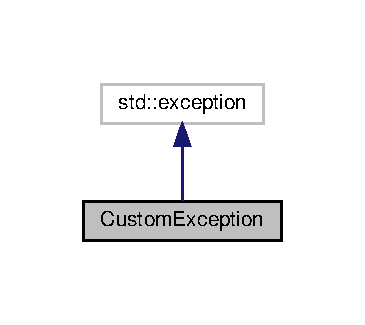
\includegraphics[width=175pt]{classCustomException__inherit__graph}
\end{center}
\end{figure}


Collaboration diagram for Custom\+Exception\+:\nopagebreak
\begin{figure}[H]
\begin{center}
\leavevmode
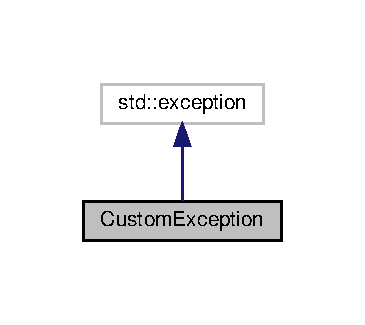
\includegraphics[width=175pt]{classCustomException__coll__graph}
\end{center}
\end{figure}
\subsection*{Public Member Functions}
\begin{DoxyCompactItemize}
\item 
\hyperlink{classCustomException_a07dbd163547759b7390b6f4588fff5a8}{Custom\+Exception} (const std\+::string \&msg=\char`\"{}Error\char`\"{})
\begin{DoxyCompactList}\small\item\em The default constructor which can set the internal message. \end{DoxyCompactList}\item 
void \hyperlink{classCustomException_a54289001348effb40f5780bb7f263abb}{Set\+Message} (const std\+::string \&msg)
\begin{DoxyCompactList}\small\item\em The aim of this function is to modify the internal message of the exception. \end{DoxyCompactList}\item 
void \hyperlink{classCustomException_ab8885c65813f31562bccdcce422b798c}{Append} (const std\+::string \&msg)
\begin{DoxyCompactList}\small\item\em This function is intended to add some text at the end of the internal message. \end{DoxyCompactList}\item 
\mbox{\Hypertarget{classCustomException_a0bb1756d6073f5bb8b6f1486b08fa5da}\label{classCustomException_a0bb1756d6073f5bb8b6f1486b08fa5da}} 
const char $\ast$ \hyperlink{classCustomException_a0bb1756d6073f5bb8b6f1486b08fa5da}{what} () const  throw ()
\begin{DoxyCompactList}\small\item\em This is a generic function for classes which manage exceptions and is intended to return the internal message as a C string ({\ttfamily char$\ast$}). \end{DoxyCompactList}\end{DoxyCompactItemize}


\subsection{Detailed Description}
A class derived from standard class {\ttfamily std\+::exception}. 

This class is customized to managed the exceptions in a desired way. This class has been defined to ease the appending of data to the message carried by an exception object. 

\subsection{Constructor \& Destructor Documentation}
\mbox{\Hypertarget{classCustomException_a07dbd163547759b7390b6f4588fff5a8}\label{classCustomException_a07dbd163547759b7390b6f4588fff5a8}} 
\index{Custom\+Exception@{Custom\+Exception}!Custom\+Exception@{Custom\+Exception}}
\index{Custom\+Exception@{Custom\+Exception}!Custom\+Exception@{Custom\+Exception}}
\subsubsection{\texorpdfstring{Custom\+Exception()}{CustomException()}}
{\footnotesize\ttfamily Custom\+Exception\+::\+Custom\+Exception (\begin{DoxyParamCaption}\item[{const std\+::string \&}]{msg = {\ttfamily \char`\"{}Error\char`\"{}} }\end{DoxyParamCaption})\hspace{0.3cm}{\ttfamily [inline]}}



The default constructor which can set the internal message. 


\begin{DoxyParams}[1]{Parameters}
\mbox{\tt in}  & {\em msg} & The internal message of the exception, which can be of type {\ttfamily char$\ast$} or {\ttfamily std\+::string}. \\
\hline
\end{DoxyParams}


\subsection{Member Function Documentation}
\mbox{\Hypertarget{classCustomException_ab8885c65813f31562bccdcce422b798c}\label{classCustomException_ab8885c65813f31562bccdcce422b798c}} 
\index{Custom\+Exception@{Custom\+Exception}!Append@{Append}}
\index{Append@{Append}!Custom\+Exception@{Custom\+Exception}}
\subsubsection{\texorpdfstring{Append()}{Append()}}
{\footnotesize\ttfamily void Custom\+Exception\+::\+Append (\begin{DoxyParamCaption}\item[{const std\+::string \&}]{msg }\end{DoxyParamCaption})\hspace{0.3cm}{\ttfamily [inline]}}



This function is intended to add some text at the end of the internal message. 


\begin{DoxyParams}[1]{Parameters}
\mbox{\tt in}  & {\em msg} & A sentence which must be appended to the internal message of the exception and which can be of type {\ttfamily char$\ast$} or {\ttfamily std\+::string}. \\
\hline
\end{DoxyParams}
\mbox{\Hypertarget{classCustomException_a54289001348effb40f5780bb7f263abb}\label{classCustomException_a54289001348effb40f5780bb7f263abb}} 
\index{Custom\+Exception@{Custom\+Exception}!Set\+Message@{Set\+Message}}
\index{Set\+Message@{Set\+Message}!Custom\+Exception@{Custom\+Exception}}
\subsubsection{\texorpdfstring{Set\+Message()}{SetMessage()}}
{\footnotesize\ttfamily void Custom\+Exception\+::\+Set\+Message (\begin{DoxyParamCaption}\item[{const std\+::string \&}]{msg }\end{DoxyParamCaption})\hspace{0.3cm}{\ttfamily [inline]}}



The aim of this function is to modify the internal message of the exception. 


\begin{DoxyParams}[1]{Parameters}
\mbox{\tt in}  & {\em msg} & The internal message of the exception, which can be of type {\ttfamily char$\ast$} or {\ttfamily std\+::string}. \\
\hline
\end{DoxyParams}


The documentation for this class was generated from the following file\+:\begin{DoxyCompactItemize}
\item 
\hyperlink{Basics_8h}{Basics.\+h}\end{DoxyCompactItemize}

\hypertarget{structData3D}{}\section{Data3D Struct Reference}
\label{structData3D}\index{Data3D@{Data3D}}


A structure intended to save the the values of the 3d sensors which are integrated in the G\+PS receiver.  




{\ttfamily \#include $<$Antenna\+Positioning.\+h$>$}

\subsection*{Public Types}
\begin{DoxyCompactItemize}
\item 
\mbox{\Hypertarget{structData3D_a1b38ab89b23a0b2b309671ac9281a2ac}\label{structData3D_a1b38ab89b23a0b2b309671ac9281a2ac}} 
enum \hyperlink{structData3D_a1b38ab89b23a0b2b309671ac9281a2ac}{Sensor\+Type} \+: char \{ {\bfseries G\+Y\+R\+O\+S\+C\+O\+PE}, 
{\bfseries C\+O\+M\+P\+A\+SS}, 
{\bfseries A\+C\+C\+E\+L\+E\+R\+O\+M\+E\+T\+ER}, 
{\bfseries U\+N\+I\+N\+I\+T\+I\+A\+L\+I\+Z\+ED}
 \}\begin{DoxyCompactList}\small\item\em An enumeration with the names of the sensors integrated in the G\+PS receiver. \end{DoxyCompactList}
\end{DoxyCompactItemize}
\subsection*{Public Attributes}
\begin{DoxyCompactItemize}
\item 
\mbox{\Hypertarget{structData3D_adf9870c0bad9cadb351fc191110549ce}\label{structData3D_adf9870c0bad9cadb351fc191110549ce}} 
\hyperlink{structData3D_a1b38ab89b23a0b2b309671ac9281a2ac}{Sensor\+Type} \hyperlink{structData3D_adf9870c0bad9cadb351fc191110549ce}{sensor}
\begin{DoxyCompactList}\small\item\em The specific sensor whose values are represented in the structure. \end{DoxyCompactList}\item 
\mbox{\Hypertarget{structData3D_a566d9370452a647cceea530cee5bb62a}\label{structData3D_a566d9370452a647cceea530cee5bb62a}} 
std\+::string \hyperlink{structData3D_a566d9370452a647cceea530cee5bb62a}{time}
\begin{DoxyCompactList}\small\item\em The time when the measurement were made, in the format H\+H\+M\+M\+S\+S.\+N\+NN, where N\+NN is a G\+PS\textquotesingle{}s internal counter that is reset when the time is updated by a new G\+PS data. \end{DoxyCompactList}\item 
\mbox{\Hypertarget{structData3D_ae8b4e2391802fc2e8b063274e6c0828e}\label{structData3D_ae8b4e2391802fc2e8b063274e6c0828e}} 
double \hyperlink{structData3D_ae8b4e2391802fc2e8b063274e6c0828e}{x}
\begin{DoxyCompactList}\small\item\em The x-\/axis value. \end{DoxyCompactList}\item 
\mbox{\Hypertarget{structData3D_a265d0776c17fba2cc402061b41853ebc}\label{structData3D_a265d0776c17fba2cc402061b41853ebc}} 
double \hyperlink{structData3D_a265d0776c17fba2cc402061b41853ebc}{y}
\begin{DoxyCompactList}\small\item\em The y-\/axis value. \end{DoxyCompactList}\item 
\mbox{\Hypertarget{structData3D_a561037592c0c27d385ddeaeb7a61f864}\label{structData3D_a561037592c0c27d385ddeaeb7a61f864}} 
double \hyperlink{structData3D_a561037592c0c27d385ddeaeb7a61f864}{z}
\begin{DoxyCompactList}\small\item\em The z-\/axis value. \end{DoxyCompactList}\end{DoxyCompactItemize}


\subsection{Detailed Description}
A structure intended to save the the values of the 3d sensors which are integrated in the G\+PS receiver. 

The documentation for this struct was generated from the following file\+:\begin{DoxyCompactItemize}
\item 
/home/new-\/mauro/eclipse-\/cdt/workspace/\+R\+F\+I\+M\+S\+\_\+\+C\+A\+R\+T/src/\hyperlink{AntennaPositioning_8h}{Antenna\+Positioning.\+h}\end{DoxyCompactItemize}

\hypertarget{classDataLogger}{}\section{Data\+Logger Class Reference}
\label{classDataLogger}\index{Data\+Logger@{Data\+Logger}}


The class {\itshape \hyperlink{classDataLogger}{Data\+Logger}} is intended to handle the storing of the generated data into memory, following the C\+SV (comma-\/separated values) format.  




{\ttfamily \#include $<$Sweep\+Processing.\+h$>$}

\subsection*{Public Member Functions}
\begin{DoxyCompactItemize}
\item 
\hyperlink{classDataLogger_a7abebacd4747644d22982f9676466bad}{Data\+Logger} ()
\begin{DoxyCompactList}\small\item\em The unique class constructor. \end{DoxyCompactList}\item 
\mbox{\Hypertarget{classDataLogger_a9aaff109f3e7749a0a0a0313655da50a}\label{classDataLogger_a9aaff109f3e7749a0a0a0313655da50a}} 
\hyperlink{classDataLogger_a9aaff109f3e7749a0a0a0313655da50a}{$\sim$\+Data\+Logger} ()
\begin{DoxyCompactList}\small\item\em The class destructor. \end{DoxyCompactList}\item 
void \hyperlink{classDataLogger_a2ffe9fb45883c2880e1c45a4406fc22b}{Save\+Bands\+Param\+As\+C\+SV} (const std\+::vector$<$ \hyperlink{structBandParameters}{Band\+Parameters} $>$ \&bands\+Param\+Vector)
\begin{DoxyCompactList}\small\item\em This method is intended to save the bands parameters in a C\+SV file which is more adequately to be read in the remote server. \end{DoxyCompactList}\item 
void \hyperlink{classDataLogger_a058ed66d04269e7d37501ecfe775c067}{Save\+Front\+End\+Param} (const \hyperlink{structFreqValues}{Freq\+Values} \&gain, const \hyperlink{structFreqValues}{Freq\+Values} \&noise\+Figure)
\begin{DoxyCompactList}\small\item\em This method is intended to save the estimated front end parameters, gain and noise figure, into the non-\/volatile memory. \end{DoxyCompactList}\item 
void \hyperlink{classDataLogger_ab2063fcd87971520a5bfa5aef6d73fea}{Save\+Sweep} (const \hyperlink{structSweep}{Sweep} \&sweep)
\begin{DoxyCompactList}\small\item\em This method is intended to save a calibrated sweep into the non-\/volatile memory. \end{DoxyCompactList}\item 
void \hyperlink{classDataLogger_a0c772c3529adc3759ba0e1e596500f65}{Save\+R\+FI} (const \hyperlink{structRFI}{R\+FI} \&rfi)
\begin{DoxyCompactList}\small\item\em This method is intended to save the detected \hyperlink{structRFI}{R\+FI} in the last sweep, into the non-\/volatile memory. \end{DoxyCompactList}\item 
\mbox{\Hypertarget{classDataLogger_a4fd6e432dd4348cbe3b02a0fd6969ab5}\label{classDataLogger_a4fd6e432dd4348cbe3b02a0fd6969ab5}} 
void \hyperlink{classDataLogger_a4fd6e432dd4348cbe3b02a0fd6969ab5}{Delete\+Old\+Files} () const
\begin{DoxyCompactList}\small\item\em The aim of this method is to delete the old files. \end{DoxyCompactList}\item 
void \hyperlink{classDataLogger_a147fb7eaee1c38bbf57ef2d6cddf70d5}{Archive\+And\+Compress} ()
\begin{DoxyCompactList}\small\item\em The aim of this method is to prepare, archive and compress, the files which will be send to the remote server. \end{DoxyCompactList}\item 
void \hyperlink{classDataLogger_ab58f4cc05f738ef757c884fe9ef131eb}{Upload\+Data} ()
\begin{DoxyCompactList}\small\item\em This method is responsible for the uploading of the data files to the remote server. \end{DoxyCompactList}\item 
void \hyperlink{classDataLogger_a98ea7aaa941bbddea8069415e1652759}{Prepare\+And\+Upload\+Data} ()
\begin{DoxyCompactList}\small\item\em This method creates a thread where the data files will be uploaded, in parallel with the capture of a new sweep. \end{DoxyCompactList}\end{DoxyCompactItemize}
\subsection*{Friends}
\begin{DoxyCompactItemize}
\item 
\mbox{\Hypertarget{classDataLogger_a0cabdadaf836f897a111e72ab29d42f6}\label{classDataLogger_a0cabdadaf836f897a111e72ab29d42f6}} 
void $\ast$ \hyperlink{classDataLogger_a0cabdadaf836f897a111e72ab29d42f6}{Upload\+Thread\+Func} (void $\ast$)
\begin{DoxyCompactList}\small\item\em The function which is executed by the thread which is responsible for the concurrent uploading of the data files. \end{DoxyCompactList}\end{DoxyCompactItemize}


\subsection{Detailed Description}
The class {\itshape \hyperlink{classDataLogger}{Data\+Logger}} is intended to handle the storing of the generated data into memory, following the C\+SV (comma-\/separated values) format. 

\subsection{Constructor \& Destructor Documentation}
\mbox{\Hypertarget{classDataLogger_a7abebacd4747644d22982f9676466bad}\label{classDataLogger_a7abebacd4747644d22982f9676466bad}} 
\index{Data\+Logger@{Data\+Logger}!Data\+Logger@{Data\+Logger}}
\index{Data\+Logger@{Data\+Logger}!Data\+Logger@{Data\+Logger}}
\subsubsection{\texorpdfstring{Data\+Logger()}{DataLogger()}}
{\footnotesize\ttfamily Data\+Logger\+::\+Data\+Logger (\begin{DoxyParamCaption}{ }\end{DoxyParamCaption})}



The unique class constructor. 

The constructor initializes all the internal attributes, checks if the corresponding folders exist and if any folder does not exist then it is created. Also, it checks if there is a shell available to be able to execute the external python script \char`\"{}client.\+py\char`\"{} to upload the data. 

\subsection{Member Function Documentation}
\mbox{\Hypertarget{classDataLogger_a147fb7eaee1c38bbf57ef2d6cddf70d5}\label{classDataLogger_a147fb7eaee1c38bbf57ef2d6cddf70d5}} 
\index{Data\+Logger@{Data\+Logger}!Archive\+And\+Compress@{Archive\+And\+Compress}}
\index{Archive\+And\+Compress@{Archive\+And\+Compress}!Data\+Logger@{Data\+Logger}}
\subsubsection{\texorpdfstring{Archive\+And\+Compress()}{ArchiveAndCompress()}}
{\footnotesize\ttfamily void Data\+Logger\+::\+Archive\+And\+Compress (\begin{DoxyParamCaption}{ }\end{DoxyParamCaption})}



The aim of this method is to prepare, archive and compress, the files which will be send to the remote server. 

To archive the data files the utility \textquotesingle{}tar\textquotesingle{} is used and thr utility \textquotesingle{}lzma\textquotesingle{} is used to compress to resulting archive file. The resulting compressed archive file is name as \char`\"{}rfims\+\_\+data\+\_\+\+D\+D-\/\+M\+M-\/\+Y\+Y\+Y\+Y\+T\+H\+H\+:\+M\+M\+:\+S\+S.\+tar.\+lzma\char`\"{}, where the last part, before the extension is the timestamp of the corresponding measurement cycle. \mbox{\Hypertarget{classDataLogger_a98ea7aaa941bbddea8069415e1652759}\label{classDataLogger_a98ea7aaa941bbddea8069415e1652759}} 
\index{Data\+Logger@{Data\+Logger}!Prepare\+And\+Upload\+Data@{Prepare\+And\+Upload\+Data}}
\index{Prepare\+And\+Upload\+Data@{Prepare\+And\+Upload\+Data}!Data\+Logger@{Data\+Logger}}
\subsubsection{\texorpdfstring{Prepare\+And\+Upload\+Data()}{PrepareAndUploadData()}}
{\footnotesize\ttfamily void Data\+Logger\+::\+Prepare\+And\+Upload\+Data (\begin{DoxyParamCaption}{ }\end{DoxyParamCaption})}



This method creates a thread where the data files will be uploaded, in parallel with the capture of a new sweep. 

This method creates a thread where the methods {\ttfamily \hyperlink{classDataLogger_a147fb7eaee1c38bbf57ef2d6cddf70d5}{Archive\+And\+Compress()}} and {\ttfamily \hyperlink{classDataLogger_ab58f4cc05f738ef757c884fe9ef131eb}{Upload\+Data()}} are called. After the creation of the thread, the method ends and the main thread can continues with the next operations, like the moving of the antenna, the capture of a new sweep, etc. The next time this method is called, it will control if the last thread has finished, if not, the method will wait to the thread to finish, and then it will create a new thread for the uploading of the new data. \mbox{\Hypertarget{classDataLogger_a2ffe9fb45883c2880e1c45a4406fc22b}\label{classDataLogger_a2ffe9fb45883c2880e1c45a4406fc22b}} 
\index{Data\+Logger@{Data\+Logger}!Save\+Bands\+Param\+As\+C\+SV@{Save\+Bands\+Param\+As\+C\+SV}}
\index{Save\+Bands\+Param\+As\+C\+SV@{Save\+Bands\+Param\+As\+C\+SV}!Data\+Logger@{Data\+Logger}}
\subsubsection{\texorpdfstring{Save\+Bands\+Param\+As\+C\+S\+V()}{SaveBandsParamAsCSV()}}
{\footnotesize\ttfamily void Data\+Logger\+::\+Save\+Bands\+Param\+As\+C\+SV (\begin{DoxyParamCaption}\item[{const std\+::vector$<$ \hyperlink{structBandParameters}{Band\+Parameters} $>$ \&}]{bands\+Param\+Vector }\end{DoxyParamCaption})}



This method is intended to save the bands parameters in a C\+SV file which is more adequately to be read in the remote server. 

This method should be called each time the bands\textquotesingle{} parameters are reloaded (or loaded by first time), because of the file \hyperlink{Basics_8h_a0423f4cb393331ce0b9f6b3a43adcaae}{B\+A\+S\+E\+\_\+\+P\+A\+TH}/parameters/freqbands.txt was modified, to update the file \hyperlink{Basics_8h_a0423f4cb393331ce0b9f6b3a43adcaae}{B\+A\+S\+E\+\_\+\+P\+A\+TH}/parameters/csv/freqbands.csv to that has the same parameters, just in a different format. The C\+SV file is generated because it is easier the bands\textquotesingle{} parameters to be loaded from a file with C\+SV format than from a file with a more human-\/readable format like freqbands.\+txt. Each time this method is called the file freqbands.\+csv is regenerated. This file is then incorporated in the archive file, in the method \hyperlink{classDataLogger_a147fb7eaee1c38bbf57ef2d6cddf70d5}{Archive\+And\+Compress()}. 
\begin{DoxyParams}[1]{Parameters}
\mbox{\tt in}  & {\em bands\+Param\+Vector} & A vector with the parameters of all frequency bands. \\
\hline
\end{DoxyParams}
\mbox{\Hypertarget{classDataLogger_a058ed66d04269e7d37501ecfe775c067}\label{classDataLogger_a058ed66d04269e7d37501ecfe775c067}} 
\index{Data\+Logger@{Data\+Logger}!Save\+Front\+End\+Param@{Save\+Front\+End\+Param}}
\index{Save\+Front\+End\+Param@{Save\+Front\+End\+Param}!Data\+Logger@{Data\+Logger}}
\subsubsection{\texorpdfstring{Save\+Front\+End\+Param()}{SaveFrontEndParam()}}
{\footnotesize\ttfamily void Data\+Logger\+::\+Save\+Front\+End\+Param (\begin{DoxyParamCaption}\item[{const \hyperlink{structFreqValues}{Freq\+Values} \&}]{gain,  }\item[{const \hyperlink{structFreqValues}{Freq\+Values} \&}]{noise\+Figure }\end{DoxyParamCaption})}



This method is intended to save the estimated front end parameters, gain and noise figure, into the non-\/volatile memory. 

The given front end parameters are saved in two different files\+:
\begin{DoxyItemize}
\item \hyperlink{Basics_8h_a0423f4cb393331ce0b9f6b3a43adcaae}{B\+A\+S\+E\+\_\+\+P\+A\+TH}/calibration/frontendparam/gain\+\_\+\+D\+D-\/\+M\+M-\/\+Y\+Y\+Y\+Y\+T\+HH\+:MM\+:S\+S.\+csv
\item \hyperlink{Basics_8h_a0423f4cb393331ce0b9f6b3a43adcaae}{B\+A\+S\+E\+\_\+\+P\+A\+TH}/calibration/frontendparam/noisefigure\+\_\+\+D\+D-\/\+M\+M-\/\+Y\+Y\+Y\+Y\+T\+HH\+:MM\+:S\+S.\+csv where D\+D-\/\+M\+M-\/\+Y\+Y\+Y\+Y\+T\+HH\+:MM\+:SS is the timestamp of the current measurement cycle.
\end{DoxyItemize}

Those files are then incorporated into the archive file which will be uploaded at the end of the measurement cycle. If the front end parameters were not estimated in a measurement cycle, then the default front end parameters are used, which are curves that were estimated in the laboratory and which are saved in the following files\+:
\begin{DoxyItemize}
\item \hyperlink{Basics_8h_a0423f4cb393331ce0b9f6b3a43adcaae}{B\+A\+S\+E\+\_\+\+P\+A\+TH}/calibration/frontendparam/default/gain\+\_\+default.csv
\item \hyperlink{Basics_8h_a0423f4cb393331ce0b9f6b3a43adcaae}{B\+A\+S\+E\+\_\+\+P\+A\+TH}/calibration/frontendparam/default/noisefigure\+\_\+default.csv In that case, these files are incorporated into the archive file to be uploaded. 
\begin{DoxyParams}[1]{Parameters}
\mbox{\tt in}  & {\em gain} & A structure with the estimated values of the total front end gain versus the frequency. \\
\hline
\mbox{\tt in}  & {\em noise\+Figure} & A structure with the estimated values of the total front end noise figure versus the frequency. \\
\hline
\end{DoxyParams}

\end{DoxyItemize}\mbox{\Hypertarget{classDataLogger_a0c772c3529adc3759ba0e1e596500f65}\label{classDataLogger_a0c772c3529adc3759ba0e1e596500f65}} 
\index{Data\+Logger@{Data\+Logger}!Save\+R\+FI@{Save\+R\+FI}}
\index{Save\+R\+FI@{Save\+R\+FI}!Data\+Logger@{Data\+Logger}}
\subsubsection{\texorpdfstring{Save\+R\+F\+I()}{SaveRFI()}}
{\footnotesize\ttfamily void Data\+Logger\+::\+Save\+R\+FI (\begin{DoxyParamCaption}\item[{const \hyperlink{structRFI}{R\+FI} \&}]{rfi }\end{DoxyParamCaption})}



This method is intended to save the detected \hyperlink{structRFI}{R\+FI} in the last sweep, into the non-\/volatile memory. 

Each given structure with the \hyperlink{structRFI}{R\+FI} detected in the last sweep is saved in a different file with the filename format R\+F\+I\+\_\+x.\+csv, where \textquotesingle{}x\textquotesingle{} is an integer number between 1 and 2$\ast$(number of azimuth positions). So each file corresponds to a sweep of the measurement cycle and all the files of determined measurement cycle are in the same folder, \hyperlink{Basics_8h_a0423f4cb393331ce0b9f6b3a43adcaae}{B\+A\+S\+E\+\_\+\+P\+A\+TH}/measurement/\+R\+F\+I\+\_\+\+D\+D-\/\+M\+M-\/\+Y\+Y\+Y\+Y\+T\+HH\+:MM\+:S\+S/ where the last part of the folder\textquotesingle{}s name is the timestamp of the measurement cycle. 
\begin{DoxyParams}[1]{Parameters}
\mbox{\tt in}  & {\em rfi} & A structure with \hyperlink{structRFI}{R\+FI} to be saved. \\
\hline
\end{DoxyParams}
\mbox{\Hypertarget{classDataLogger_ab2063fcd87971520a5bfa5aef6d73fea}\label{classDataLogger_ab2063fcd87971520a5bfa5aef6d73fea}} 
\index{Data\+Logger@{Data\+Logger}!Save\+Sweep@{Save\+Sweep}}
\index{Save\+Sweep@{Save\+Sweep}!Data\+Logger@{Data\+Logger}}
\subsubsection{\texorpdfstring{Save\+Sweep()}{SaveSweep()}}
{\footnotesize\ttfamily void Data\+Logger\+::\+Save\+Sweep (\begin{DoxyParamCaption}\item[{const \hyperlink{structSweep}{Sweep} \&}]{sweep }\end{DoxyParamCaption})}



This method is intended to save a calibrated sweep into the non-\/volatile memory. 

The given sweep is saved in \hyperlink{Basics_8h_a0423f4cb393331ce0b9f6b3a43adcaae}{B\+A\+S\+E\+\_\+\+P\+A\+TH}/measurements/ with the filename format \char`\"{}sweep\+\_\+\+D\+D-\/\+M\+M-\/\+Y\+Y\+Y\+Y\+T\+H\+H\+:\+M\+M\+:\+S\+S.\+csv\char`\"{} where the last part is the timestamp of the measurement cycle, which correspond to the beginning of this one.

All sweeps which corresponds to the same measurement cycle are saved in the same file and the method automatically create a new file or reopen the corresponding file each time a new sweep must be saved. 
\begin{DoxyParams}[1]{Parameters}
\mbox{\tt in}  & {\em sweep} & A structure with the sweep to be saved. \\
\hline
\end{DoxyParams}
\mbox{\Hypertarget{classDataLogger_ab58f4cc05f738ef757c884fe9ef131eb}\label{classDataLogger_ab58f4cc05f738ef757c884fe9ef131eb}} 
\index{Data\+Logger@{Data\+Logger}!Upload\+Data@{Upload\+Data}}
\index{Upload\+Data@{Upload\+Data}!Data\+Logger@{Data\+Logger}}
\subsubsection{\texorpdfstring{Upload\+Data()}{UploadData()}}
{\footnotesize\ttfamily void Data\+Logger\+::\+Upload\+Data (\begin{DoxyParamCaption}{ }\end{DoxyParamCaption})}



This method is responsible for the uploading of the data files to the remote server. 

To upload the files the script /usr/local/client.py is called. This script try to send the archive file many times through one hour, taking into account the possibility that there is no Internet connection in the first try. If the script achieves the sending, then it wakes up the remote server to that one to read the files, and finally the script removes the local archive file. If the script ends with errors, the file is not deleted and remains in a queue waiting to be send. The idea is the uploading to perform at the end of each measurement cycle. 

The documentation for this class was generated from the following files\+:\begin{DoxyCompactItemize}
\item 
/home/new-\/mauro/eclipse-\/cdt/workspace/\+R\+F\+I\+M\+S\+\_\+\+C\+A\+R\+T/src/\hyperlink{SweepProcessing_8h}{Sweep\+Processing.\+h}\item 
/home/new-\/mauro/eclipse-\/cdt/workspace/\+R\+F\+I\+M\+S\+\_\+\+C\+A\+R\+T/src/\hyperlink{DataLogger_8cpp}{Data\+Logger.\+cpp}\end{DoxyCompactItemize}

\hypertarget{structSpectranConfigurator_1_1FixedParameters}{}\section{Spectran\+Configurator\+:\+:Fixed\+Parameters Struct Reference}
\label{structSpectranConfigurator_1_1FixedParameters}\index{Spectran\+Configurator\+::\+Fixed\+Parameters@{Spectran\+Configurator\+::\+Fixed\+Parameters}}


This structure saves the fixed parameters of the spectrum analyzer, i.\+e. the parameters which do not change through the entire measurement cycle.  




{\ttfamily \#include $<$Spectran.\+h$>$}

\subsection*{Public Attributes}
\begin{DoxyCompactItemize}
\item 
\mbox{\Hypertarget{structSpectranConfigurator_1_1FixedParameters_aa5eb199d61f2c5763e32b70d2bf7c368}\label{structSpectranConfigurator_1_1FixedParameters_aa5eb199d61f2c5763e32b70d2bf7c368}} 
int \hyperlink{structSpectranConfigurator_1_1FixedParameters_aa5eb199d61f2c5763e32b70d2bf7c368}{atten\+Factor}
\begin{DoxyCompactList}\small\item\em Attenuator factor \mbox{[}dB\mbox{]}\+: -\/10=auto, 0=off or a value between 1 to 30. \end{DoxyCompactList}\item 
\mbox{\Hypertarget{structSpectranConfigurator_1_1FixedParameters_ad8a37b8a7981c811f1e8f89770ba2a7d}\label{structSpectranConfigurator_1_1FixedParameters_ad8a37b8a7981c811f1e8f89770ba2a7d}} 
unsigned int \hyperlink{structSpectranConfigurator_1_1FixedParameters_ad8a37b8a7981c811f1e8f89770ba2a7d}{display\+Unit}
\begin{DoxyCompactList}\small\item\em Measurement unit\+: 0=d\+Bm (power), 1=d\+BuV (voltage), 2=V/m (electric field strength) or 3=A/m (magnetic field strength). \end{DoxyCompactList}\item 
\mbox{\Hypertarget{structSpectranConfigurator_1_1FixedParameters_ad9255da208ff6b07f5a591f3dea22f84}\label{structSpectranConfigurator_1_1FixedParameters_ad9255da208ff6b07f5a591f3dea22f84}} 
const unsigned int \hyperlink{structSpectranConfigurator_1_1FixedParameters_ad9255da208ff6b07f5a591f3dea22f84}{demod\+Mode} =0
\begin{DoxyCompactList}\small\item\em Demodulator mode\+: 0=off, 1=am or 2=fm. \end{DoxyCompactList}\item 
\mbox{\Hypertarget{structSpectranConfigurator_1_1FixedParameters_a29f211747f28dc036ac1e8d894db7dd4}\label{structSpectranConfigurator_1_1FixedParameters_a29f211747f28dc036ac1e8d894db7dd4}} 
unsigned int \hyperlink{structSpectranConfigurator_1_1FixedParameters_a29f211747f28dc036ac1e8d894db7dd4}{antenna\+Type}
\begin{DoxyCompactList}\small\item\em Antenna type\+: 0=H\+L7025, 1=H\+L7040, 2=H\+L7060, 3=H\+L6080 or 4=H60100. \end{DoxyCompactList}\item 
\mbox{\Hypertarget{structSpectranConfigurator_1_1FixedParameters_af1eeef76fb85a2ccf937f3dd949d9980}\label{structSpectranConfigurator_1_1FixedParameters_af1eeef76fb85a2ccf937f3dd949d9980}} 
int \hyperlink{structSpectranConfigurator_1_1FixedParameters_af1eeef76fb85a2ccf937f3dd949d9980}{cable\+Type}
\begin{DoxyCompactList}\small\item\em Cable type\+: -\/1 is none, 0 is “1m standard cable”. \end{DoxyCompactList}\item 
\mbox{\Hypertarget{structSpectranConfigurator_1_1FixedParameters_a212370cc31cf311edf1ce71ca01f4b91}\label{structSpectranConfigurator_1_1FixedParameters_a212370cc31cf311edf1ce71ca01f4b91}} 
const unsigned int \hyperlink{structSpectranConfigurator_1_1FixedParameters_a212370cc31cf311edf1ce71ca01f4b91}{recv\+Conf} =0
\begin{DoxyCompactList}\small\item\em Receiver configuration\+: 0=spectrum, 1=broadband. \end{DoxyCompactList}\item 
\mbox{\Hypertarget{structSpectranConfigurator_1_1FixedParameters_aa86943c70f5c03d87fb78c05af17ac28}\label{structSpectranConfigurator_1_1FixedParameters_aa86943c70f5c03d87fb78c05af17ac28}} 
bool \hyperlink{structSpectranConfigurator_1_1FixedParameters_aa86943c70f5c03d87fb78c05af17ac28}{intern\+Preamp}
\begin{DoxyCompactList}\small\item\em Internal preamplifier enabling\+: 0=off, 1=on. \end{DoxyCompactList}\item 
\mbox{\Hypertarget{structSpectranConfigurator_1_1FixedParameters_ad835d567560a9fb3bf1f9469955c2363}\label{structSpectranConfigurator_1_1FixedParameters_ad835d567560a9fb3bf1f9469955c2363}} 
bool \hyperlink{structSpectranConfigurator_1_1FixedParameters_ad835d567560a9fb3bf1f9469955c2363}{sweep\+Delay\+Acc}
\begin{DoxyCompactList}\small\item\em \hyperlink{structSweep}{Sweep} delay for accuracy mode\+: 1=enable, 0=disable. \end{DoxyCompactList}\item 
\mbox{\Hypertarget{structSpectranConfigurator_1_1FixedParameters_a5d0c325f17d9e3efce429b187c833911}\label{structSpectranConfigurator_1_1FixedParameters_a5d0c325f17d9e3efce429b187c833911}} 
const bool \hyperlink{structSpectranConfigurator_1_1FixedParameters_a5d0c325f17d9e3efce429b187c833911}{peak\+Level\+Audio\+Tone} =0
\begin{DoxyCompactList}\small\item\em Peak Level Audio tone\+: 0=disable, 1=enable. \end{DoxyCompactList}\item 
\mbox{\Hypertarget{structSpectranConfigurator_1_1FixedParameters_ad20c44e63927366260399b4ffa5a32d9}\label{structSpectranConfigurator_1_1FixedParameters_ad20c44e63927366260399b4ffa5a32d9}} 
const bool \hyperlink{structSpectranConfigurator_1_1FixedParameters_ad20c44e63927366260399b4ffa5a32d9}{back\+B\+B\+Detector} =0
\begin{DoxyCompactList}\small\item\em Background Broadband detector\+: 0=disable, 1=enable. \end{DoxyCompactList}\item 
\mbox{\Hypertarget{structSpectranConfigurator_1_1FixedParameters_a4b30a0ba5199d6c6703838142da3bcdc}\label{structSpectranConfigurator_1_1FixedParameters_a4b30a0ba5199d6c6703838142da3bcdc}} 
float \hyperlink{structSpectranConfigurator_1_1FixedParameters_a4b30a0ba5199d6c6703838142da3bcdc}{speaker\+Vol}
\begin{DoxyCompactList}\small\item\em Speaker volume\+: range from 0.\+0 to 1.\+0. \end{DoxyCompactList}\end{DoxyCompactItemize}


\subsection{Detailed Description}
This structure saves the fixed parameters of the spectrum analyzer, i.\+e. the parameters which do not change through the entire measurement cycle. 

The documentation for this struct was generated from the following file\+:\begin{DoxyCompactItemize}
\item 
/home/new-\/mauro/eclipse-\/cdt/workspace/\+R\+F\+I\+M\+S\+\_\+\+C\+A\+R\+T/src/\hyperlink{Spectran_8h}{Spectran.\+h}\end{DoxyCompactItemize}

\hypertarget{unionFloatToBytes}{}\section{Float\+To\+Bytes Union Reference}
\label{unionFloatToBytes}\index{Float\+To\+Bytes@{Float\+To\+Bytes}}


An union which is used to split a {\ttfamily float} value in its 4 bytes.  




{\ttfamily \#include $<$Spectran.\+h$>$}

\subsection*{Public Attributes}
\begin{DoxyCompactItemize}
\item 
\mbox{\Hypertarget{unionFloatToBytes_a446d779e6c020ceb138be65a8b5bb7fb}\label{unionFloatToBytes_a446d779e6c020ceb138be65a8b5bb7fb}} 
float \hyperlink{unionFloatToBytes_a446d779e6c020ceb138be65a8b5bb7fb}{float\+Value}
\begin{DoxyCompactList}\small\item\em The {\ttfamily float} value which must be split. \end{DoxyCompactList}\item 
\mbox{\Hypertarget{unionFloatToBytes_adc2324525bc45e5052501c6650b5afb6}\label{unionFloatToBytes_adc2324525bc45e5052501c6650b5afb6}} 
std\+::uint8\+\_\+t \hyperlink{unionFloatToBytes_adc2324525bc45e5052501c6650b5afb6}{bytes} \mbox{[}4\mbox{]}
\begin{DoxyCompactList}\small\item\em The array with the 4 bytes of the inserted {\ttfamily float} value. \end{DoxyCompactList}\end{DoxyCompactItemize}


\subsection{Detailed Description}
An union which is used to split a {\ttfamily float} value in its 4 bytes. 

The documentation for this union was generated from the following file\+:\begin{DoxyCompactItemize}
\item 
\hyperlink{Spectran_8h}{Spectran.\+h}\end{DoxyCompactItemize}

\hypertarget{structFreqValues}{}\section{Freq\+Values Struct Reference}
\label{structFreqValues}\index{Freq\+Values@{Freq\+Values}}


The aim of this structure is to store the curve of a determined parameter or variable versus the frequency, which is named a frequency curve here.  




{\ttfamily \#include $<$Basics.\+h$>$}



Inheritance diagram for Freq\+Values\+:\nopagebreak
\begin{figure}[H]
\begin{center}
\leavevmode
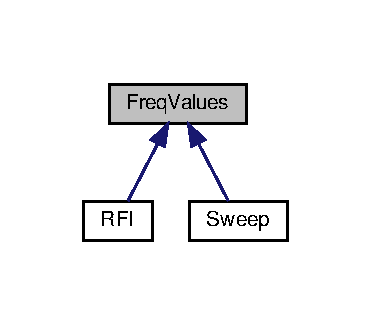
\includegraphics[width=178pt]{structFreqValues__inherit__graph}
\end{center}
\end{figure}


Collaboration diagram for Freq\+Values\+:\nopagebreak
\begin{figure}[H]
\begin{center}
\leavevmode
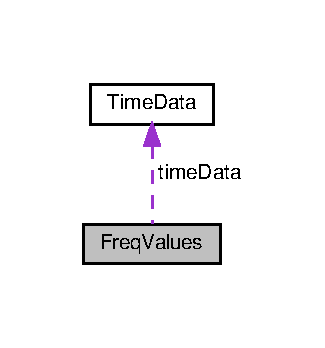
\includegraphics[width=156pt]{structFreqValues__coll__graph}
\end{center}
\end{figure}
\subsection*{Public Member Functions}
\begin{DoxyCompactItemize}
\item 
\hyperlink{structFreqValues_ab2ff89efb4571a8f6748017c6191d81e}{Freq\+Values} (const std\+::string \&typ=\char`\"{}unknown\char`\"{})
\begin{DoxyCompactList}\small\item\em The default constructor which can receive the curve type. \end{DoxyCompactList}\item 
\hyperlink{structFreqValues_a7061709cf9faa8e7ee6cf2d15fd30a66}{Freq\+Values} (const \hyperlink{structFreqValues}{Freq\+Values} \&freq\+Values)
\begin{DoxyCompactList}\small\item\em The copy constructor. \end{DoxyCompactList}\item 
\mbox{\Hypertarget{structFreqValues_a6ec6ba96834034b3b91d1519b90027b7}\label{structFreqValues_a6ec6ba96834034b3b91d1519b90027b7}} 
virtual \hyperlink{structFreqValues_a6ec6ba96834034b3b91d1519b90027b7}{$\sim$\+Freq\+Values} ()
\begin{DoxyCompactList}\small\item\em This is the structure\textquotesingle{}s destructor which is virtual because there are structures derived from this structure. \end{DoxyCompactList}\item 
bool \hyperlink{structFreqValues_a01315cf6bb4ed4e21ee1b6441c44a850}{Push\+Back} (const \hyperlink{structFreqValues}{Freq\+Values} \&freq\+Values)
\begin{DoxyCompactList}\small\item\em This method is intended to insert one data point (frequency,value) or a set of data points in the structure, at the end. \end{DoxyCompactList}\item 
\mbox{\Hypertarget{structFreqValues_ad47dd37005ced2182e9be2a1e16cd702}\label{structFreqValues_ad47dd37005ced2182e9be2a1e16cd702}} 
virtual void \hyperlink{structFreqValues_ad47dd37005ced2182e9be2a1e16cd702}{Clear} ()
\begin{DoxyCompactList}\small\item\em This method is intended to clear the structure, i.\+e. to delete all its data points. \end{DoxyCompactList}\item 
\mbox{\Hypertarget{structFreqValues_ae5a9b788cbf75ad4c3e1dd1ed86a0ddc}\label{structFreqValues_ae5a9b788cbf75ad4c3e1dd1ed86a0ddc}} 
bool \hyperlink{structFreqValues_ae5a9b788cbf75ad4c3e1dd1ed86a0ddc}{Empty} () const
\begin{DoxyCompactList}\small\item\em This method allows to know if the structure is empty, i.\+e. it has no data points. \end{DoxyCompactList}\item 
const \hyperlink{structFreqValues}{Freq\+Values} \& \hyperlink{structFreqValues_a11021e293ec300860ffc503d3c37a58c}{operator=} (const \hyperlink{structFreqValues}{Freq\+Values} \&freq\+Values)
\begin{DoxyCompactList}\small\item\em An overloading of the assignment operator adapted for this structure. \end{DoxyCompactList}\item 
const \hyperlink{structFreqValues}{Freq\+Values} \& \hyperlink{structFreqValues_a8024942907aaf5fd4aaa49850bbe6cd5}{operator+=} (const \hyperlink{structFreqValues}{Freq\+Values} \&rhs)
\begin{DoxyCompactList}\small\item\em An overloading of the operator += adapted for this structure. \end{DoxyCompactList}\item 
\mbox{\Hypertarget{structFreqValues_a954b961f99175f11f09d1cd5d834c545}\label{structFreqValues_a954b961f99175f11f09d1cd5d834c545}} 
float \hyperlink{structFreqValues_a954b961f99175f11f09d1cd5d834c545}{Mean\+Value} () const
\begin{DoxyCompactList}\small\item\em The aim of this method is to offer the mean value of all data points, i.\+e. it calculates the average. \end{DoxyCompactList}\end{DoxyCompactItemize}
\subsection*{Public Attributes}
\begin{DoxyCompactItemize}
\item 
\mbox{\Hypertarget{structFreqValues_a457f391fad53ee1e8bca839dde90c5f1}\label{structFreqValues_a457f391fad53ee1e8bca839dde90c5f1}} 
std\+::string \hyperlink{structFreqValues_a457f391fad53ee1e8bca839dde90c5f1}{type}
\begin{DoxyCompactList}\small\item\em Type of frequency values\+: ”sweep”, “frequency response”, “calibration curve”, “threshold curve”, “rfi", etc. \end{DoxyCompactList}\item 
\mbox{\Hypertarget{structFreqValues_a07669bbe3b65cbfb80300631ce85fb76}\label{structFreqValues_a07669bbe3b65cbfb80300631ce85fb76}} 
std\+::vector$<$ float $>$ \hyperlink{structFreqValues_a07669bbe3b65cbfb80300631ce85fb76}{values}
\begin{DoxyCompactList}\small\item\em RF power values (d\+Bm), gain values (dB or d\+Bi), noise figure values (dB), etc. \end{DoxyCompactList}\item 
\mbox{\Hypertarget{structFreqValues_a2b625831a46019f93a0999c1bed5c3a0}\label{structFreqValues_a2b625831a46019f93a0999c1bed5c3a0}} 
std\+::vector$<$ std\+::uint\+\_\+least64\+\_\+t $>$ \hyperlink{structFreqValues_a2b625831a46019f93a0999c1bed5c3a0}{frequencies}
\begin{DoxyCompactList}\small\item\em Frequency values in Hz. \end{DoxyCompactList}\item 
\hyperlink{structTimeData}{Time\+Data} \hyperlink{structFreqValues_a4c97a4710c83078f5af5d92f2bedfe61}{time\+Data}
\end{DoxyCompactItemize}
\subsection*{Friends}
\begin{DoxyCompactItemize}
\item 
\hyperlink{structFreqValues}{Freq\+Values} \hyperlink{structFreqValues_af2d38eb1ad1d3c6dfab8b4ea399c867d}{operator-\/} (const \hyperlink{structFreqValues}{Freq\+Values} \&argument)
\begin{DoxyCompactList}\small\item\em An overloading of the unary operator -\/ which negates a {\itshape \hyperlink{structFreqValues}{Freq\+Values}} object. \end{DoxyCompactList}\item 
\hyperlink{structFreqValues}{Freq\+Values} \hyperlink{structFreqValues_aa27b2370e9b314e6e0f308f4efb39a2f}{operator+} (const \hyperlink{structFreqValues}{Freq\+Values} \&lhs, const \hyperlink{structFreqValues}{Freq\+Values} \&rhs)
\begin{DoxyCompactList}\small\item\em An overloading of operator + which calculates the sum of two objects of structure {\itshape \hyperlink{structFreqValues}{Freq\+Values}}. \end{DoxyCompactList}\item 
\hyperlink{structFreqValues}{Freq\+Values} \hyperlink{structFreqValues_afa29d8e6cf56d1c724c712bcc95c0e4b}{operator+} (const \hyperlink{structFreqValues}{Freq\+Values} \&lhs, const float rhs)
\begin{DoxyCompactList}\small\item\em An overloading of operator + which calculates the sum of a {\itshape \hyperlink{structFreqValues}{Freq\+Values}} object and a {\itshape float} value, in that order. \end{DoxyCompactList}\item 
\hyperlink{structFreqValues}{Freq\+Values} \hyperlink{structFreqValues_add1a78bbae864d4a24ac7b491ae41b2e}{operator+} (const float lhs, const \hyperlink{structFreqValues}{Freq\+Values} \&rhs)
\begin{DoxyCompactList}\small\item\em An overloading of operator + which calculates the sum of a {\itshape float} value and a {\itshape \hyperlink{structFreqValues}{Freq\+Values}} object, in that order. \end{DoxyCompactList}\item 
\hyperlink{structFreqValues}{Freq\+Values} \hyperlink{structFreqValues_a05184c79e4dadc7a4e1f3a76fba1c3c8}{operator-\/} (const \hyperlink{structFreqValues}{Freq\+Values} \&lhs, const \hyperlink{structFreqValues}{Freq\+Values} \&rhs)
\begin{DoxyCompactList}\small\item\em An overloading of operator -\/ which calculates the subtraction of two objects of structure {\itshape \hyperlink{structFreqValues}{Freq\+Values}}. \end{DoxyCompactList}\item 
\hyperlink{structFreqValues}{Freq\+Values} \hyperlink{structFreqValues_ade558a5146a3dbea46f85e64d959ff3d}{operator-\/} (const \hyperlink{structFreqValues}{Freq\+Values} \&lhs, const float rhs)
\begin{DoxyCompactList}\small\item\em An overloading of operator -\/ which calculates the subtraction of a {\itshape \hyperlink{structFreqValues}{Freq\+Values}} object and a {\itshape float} value, in that order. \end{DoxyCompactList}\item 
\hyperlink{structFreqValues}{Freq\+Values} \hyperlink{structFreqValues_aa248d5bc83ba0c614137b042947064a8}{operator-\/} (const float lhs, const \hyperlink{structFreqValues}{Freq\+Values} \&rhs)
\begin{DoxyCompactList}\small\item\em An overloading of operator -\/ which calculates the subtraction of a {\itshape float} value and a {\itshape \hyperlink{structFreqValues}{Freq\+Values}} object, in that order. \end{DoxyCompactList}\item 
\hyperlink{structFreqValues}{Freq\+Values} \hyperlink{structFreqValues_a3e567844a5d4347e3b30e696132bfb7c}{operator$\ast$} (const \hyperlink{structFreqValues}{Freq\+Values} \&lhs, const \hyperlink{structFreqValues}{Freq\+Values} \&rhs)
\begin{DoxyCompactList}\small\item\em An overloading of operator $\ast$ which multiplies two objects of structure {\itshape \hyperlink{structFreqValues}{Freq\+Values}}. \end{DoxyCompactList}\item 
\hyperlink{structFreqValues}{Freq\+Values} \hyperlink{structFreqValues_aea565aadf51307e09845c72179e5082d}{operator$\ast$} (const \hyperlink{structFreqValues}{Freq\+Values} \&lhs, const float rhs)
\begin{DoxyCompactList}\small\item\em An overloading of operator $\ast$ which multiplies a {\itshape \hyperlink{structFreqValues}{Freq\+Values}} object and a {\itshape float} value, in that order. \end{DoxyCompactList}\item 
\hyperlink{structFreqValues}{Freq\+Values} \hyperlink{structFreqValues_ab9bb62425b97f45a5eb485cf745bfe4a}{operator$\ast$} (const float lhs, const \hyperlink{structFreqValues}{Freq\+Values} \&rhs)
\begin{DoxyCompactList}\small\item\em An overloading of operator $\ast$ which multiplies a {\itshape float} value and a {\itshape \hyperlink{structFreqValues}{Freq\+Values}} object, in that order. \end{DoxyCompactList}\item 
\hyperlink{structFreqValues}{Freq\+Values} \hyperlink{structFreqValues_a26f13922dd72ad292bea45072abc2c96}{operator/} (const \hyperlink{structFreqValues}{Freq\+Values} \&lhs, const \hyperlink{structFreqValues}{Freq\+Values} \&rhs)
\begin{DoxyCompactList}\small\item\em An overloading of operator / which calculates the division between two objects of structure {\itshape \hyperlink{structFreqValues}{Freq\+Values}}. \end{DoxyCompactList}\item 
\hyperlink{structFreqValues}{Freq\+Values} \hyperlink{structFreqValues_a392b5ed122a4deafa3ba773f4829c20a}{operator/} (const \hyperlink{structFreqValues}{Freq\+Values} \&lhs, const float rhs)
\begin{DoxyCompactList}\small\item\em An overloading of operator / which calculates the division between a {\itshape \hyperlink{structFreqValues}{Freq\+Values}} object and a {\itshape float} value, in that order. \end{DoxyCompactList}\item 
\hyperlink{structFreqValues}{Freq\+Values} \hyperlink{structFreqValues_aed1d809f52aa8f6da3afa2af8a45d288}{operator/} (const float lhs, const \hyperlink{structFreqValues}{Freq\+Values} \&rhs)
\begin{DoxyCompactList}\small\item\em An overloading of operator / which calculates the division between a {\itshape float} value and a {\itshape \hyperlink{structFreqValues}{Freq\+Values}} object, in that order. \end{DoxyCompactList}\item 
\hyperlink{structFreqValues}{Freq\+Values} \hyperlink{structFreqValues_a90781867604621a99e59d4fcdc4a5f38}{log10} (const \hyperlink{structFreqValues}{Freq\+Values} \&argument)
\begin{DoxyCompactList}\small\item\em An overloading of function {\ttfamily \hyperlink{structFreqValues_a90781867604621a99e59d4fcdc4a5f38}{log10()}}, decimal logarithm, adapted to receive an argument of type {\itshape \hyperlink{structFreqValues}{Freq\+Values}}. \end{DoxyCompactList}\item 
\hyperlink{structFreqValues}{Freq\+Values} \hyperlink{structFreqValues_a8b8ee90b9d108ad7008a3613b31253e7}{pow} (const \hyperlink{structFreqValues}{Freq\+Values} \&base, const float exponent)
\begin{DoxyCompactList}\small\item\em An overloading of function {\ttfamily \hyperlink{structFreqValues_a8b8ee90b9d108ad7008a3613b31253e7}{pow()}}, power function, adapted to receive an argument of type {\itshape \hyperlink{structFreqValues}{Freq\+Values}} as base and an argument of type {\itshape float} as exponent. \end{DoxyCompactList}\item 
\hyperlink{structFreqValues}{Freq\+Values} \hyperlink{structFreqValues_a4a50ddd9aa3d48c0b3da456ca07551a5}{pow} (const float base, const \hyperlink{structFreqValues}{Freq\+Values} \&exponent)
\begin{DoxyCompactList}\small\item\em An overloading of function {\ttfamily \hyperlink{structFreqValues_a8b8ee90b9d108ad7008a3613b31253e7}{pow()}}, exponentiation, adapted to receive an argument of type {\itshape float} as base and an argument of type {\itshape \hyperlink{structFreqValues}{Freq\+Values}} as exponent. \end{DoxyCompactList}\end{DoxyCompactItemize}


\subsection{Detailed Description}
The aim of this structure is to store the curve of a determined parameter or variable versus the frequency, which is named a frequency curve here. 

\subsection{Constructor \& Destructor Documentation}
\mbox{\Hypertarget{structFreqValues_ab2ff89efb4571a8f6748017c6191d81e}\label{structFreqValues_ab2ff89efb4571a8f6748017c6191d81e}} 
\index{Freq\+Values@{Freq\+Values}!Freq\+Values@{Freq\+Values}}
\index{Freq\+Values@{Freq\+Values}!Freq\+Values@{Freq\+Values}}
\subsubsection{\texorpdfstring{Freq\+Values()}{FreqValues()}\hspace{0.1cm}{\footnotesize\ttfamily [1/2]}}
{\footnotesize\ttfamily Freq\+Values\+::\+Freq\+Values (\begin{DoxyParamCaption}\item[{const std\+::string \&}]{typ = {\ttfamily \char`\"{}unknown\char`\"{}} }\end{DoxyParamCaption})\hspace{0.3cm}{\ttfamily [inline]}}



The default constructor which can receive the curve type. 


\begin{DoxyParams}[1]{Parameters}
\mbox{\tt in}  & {\em typ} & The type of parameter whose curve of values versus frequency is stored in the structure. \\
\hline
\end{DoxyParams}
\mbox{\Hypertarget{structFreqValues_a7061709cf9faa8e7ee6cf2d15fd30a66}\label{structFreqValues_a7061709cf9faa8e7ee6cf2d15fd30a66}} 
\index{Freq\+Values@{Freq\+Values}!Freq\+Values@{Freq\+Values}}
\index{Freq\+Values@{Freq\+Values}!Freq\+Values@{Freq\+Values}}
\subsubsection{\texorpdfstring{Freq\+Values()}{FreqValues()}\hspace{0.1cm}{\footnotesize\ttfamily [2/2]}}
{\footnotesize\ttfamily Freq\+Values\+::\+Freq\+Values (\begin{DoxyParamCaption}\item[{const \hyperlink{structFreqValues}{Freq\+Values} \&}]{freq\+Values }\end{DoxyParamCaption})\hspace{0.3cm}{\ttfamily [inline]}}



The copy constructor. 


\begin{DoxyParams}[1]{Parameters}
\mbox{\tt in}  & {\em freq\+Values} & Another {\itshape \hyperlink{structFreqValues}{Freq\+Values}} structure which is given to copy its attributes. \\
\hline
\end{DoxyParams}


\subsection{Member Function Documentation}
\mbox{\Hypertarget{structFreqValues_a8024942907aaf5fd4aaa49850bbe6cd5}\label{structFreqValues_a8024942907aaf5fd4aaa49850bbe6cd5}} 
\index{Freq\+Values@{Freq\+Values}!operator+=@{operator+=}}
\index{operator+=@{operator+=}!Freq\+Values@{Freq\+Values}}
\subsubsection{\texorpdfstring{operator+=()}{operator+=()}}
{\footnotesize\ttfamily const \hyperlink{structFreqValues}{Freq\+Values} \& Freq\+Values\+::operator+= (\begin{DoxyParamCaption}\item[{const \hyperlink{structFreqValues}{Freq\+Values} \&}]{rhs }\end{DoxyParamCaption})}



An overloading of the operator += adapted for this structure. 

This method is not intended to concatenate two {\itshape \hyperlink{structFreqValues}{Freq\+Values}} structure, what is performed by the method {\ttfamily \hyperlink{structFreqValues_a01315cf6bb4ed4e21ee1b6441c44a850}{Push\+Back()}}, but its aim is to sum each point of base structure with the corresponding point of the structure given as argument, and to save the results in the base structure.

The method returns a {\ttfamily const} reference to the base structure. 
\begin{DoxyParams}[1]{Parameters}
\mbox{\tt in}  & {\em rhs} & A {\itshape \hyperlink{structFreqValues}{Freq\+Values}} structure which is given to perform the sum. \\
\hline
\end{DoxyParams}
\mbox{\Hypertarget{structFreqValues_a11021e293ec300860ffc503d3c37a58c}\label{structFreqValues_a11021e293ec300860ffc503d3c37a58c}} 
\index{Freq\+Values@{Freq\+Values}!operator=@{operator=}}
\index{operator=@{operator=}!Freq\+Values@{Freq\+Values}}
\subsubsection{\texorpdfstring{operator=()}{operator=()}}
{\footnotesize\ttfamily const \hyperlink{structFreqValues}{Freq\+Values} \& Freq\+Values\+::operator= (\begin{DoxyParamCaption}\item[{const \hyperlink{structFreqValues}{Freq\+Values} \&}]{freq\+Values }\end{DoxyParamCaption})}



An overloading of the assignment operator adapted for this structure. 

The method returns a {\ttfamily const} reference to the base structure. 
\begin{DoxyParams}[1]{Parameters}
\mbox{\tt in}  & {\em freq\+Values} & Another {\itshape \hyperlink{structFreqValues}{Freq\+Values}} structure which is given to copy its attributes. \\
\hline
\end{DoxyParams}
\mbox{\Hypertarget{structFreqValues_a01315cf6bb4ed4e21ee1b6441c44a850}\label{structFreqValues_a01315cf6bb4ed4e21ee1b6441c44a850}} 
\index{Freq\+Values@{Freq\+Values}!Push\+Back@{Push\+Back}}
\index{Push\+Back@{Push\+Back}!Freq\+Values@{Freq\+Values}}
\subsubsection{\texorpdfstring{Push\+Back()}{PushBack()}}
{\footnotesize\ttfamily bool Freq\+Values\+::\+Push\+Back (\begin{DoxyParamCaption}\item[{const \hyperlink{structFreqValues}{Freq\+Values} \&}]{freq\+Values }\end{DoxyParamCaption})}



This method is intended to insert one data point (frequency,value) or a set of data points in the structure, at the end. 


\begin{DoxyParams}[1]{Parameters}
\mbox{\tt in}  & {\em freq\+Values} & Another {\itshape \hyperlink{structFreqValues}{Freq\+Values}} structure whose values must be inserted at the end of this structure. \\
\hline
\end{DoxyParams}


\subsection{Friends And Related Function Documentation}
\mbox{\Hypertarget{structFreqValues_a90781867604621a99e59d4fcdc4a5f38}\label{structFreqValues_a90781867604621a99e59d4fcdc4a5f38}} 
\index{Freq\+Values@{Freq\+Values}!log10@{log10}}
\index{log10@{log10}!Freq\+Values@{Freq\+Values}}
\subsubsection{\texorpdfstring{log10}{log10}}
{\footnotesize\ttfamily \hyperlink{structFreqValues}{Freq\+Values} log10 (\begin{DoxyParamCaption}\item[{const \hyperlink{structFreqValues}{Freq\+Values} \&}]{argument }\end{DoxyParamCaption})\hspace{0.3cm}{\ttfamily [friend]}}



An overloading of function {\ttfamily \hyperlink{structFreqValues_a90781867604621a99e59d4fcdc4a5f38}{log10()}}, decimal logarithm, adapted to receive an argument of type {\itshape \hyperlink{structFreqValues}{Freq\+Values}}. 

This function takes each point of the given structure, apply the decimal logarithm whit its value and stores the result in a different {\itshape \hyperlink{structFreqValues}{Freq\+Values}} structure, which is then returned. The rest of attributes (frequency, type, timestamp, etc.) are copied as-\/is to the object to be returned. 
\begin{DoxyParams}[1]{Parameters}
\mbox{\tt in}  & {\em argument} & The {\itshape \hyperlink{structFreqValues}{Freq\+Values}} structure to be used as argument to the decimal logarithm operation. \\
\hline
\end{DoxyParams}
\mbox{\Hypertarget{structFreqValues_a3e567844a5d4347e3b30e696132bfb7c}\label{structFreqValues_a3e567844a5d4347e3b30e696132bfb7c}} 
\index{Freq\+Values@{Freq\+Values}!operator$\ast$@{operator$\ast$}}
\index{operator$\ast$@{operator$\ast$}!Freq\+Values@{Freq\+Values}}
\subsubsection{\texorpdfstring{operator$\ast$}{operator*}\hspace{0.1cm}{\footnotesize\ttfamily [1/3]}}
{\footnotesize\ttfamily \hyperlink{structFreqValues}{Freq\+Values} operator$\ast$ (\begin{DoxyParamCaption}\item[{const \hyperlink{structFreqValues}{Freq\+Values} \&}]{lhs,  }\item[{const \hyperlink{structFreqValues}{Freq\+Values} \&}]{rhs }\end{DoxyParamCaption})\hspace{0.3cm}{\ttfamily [friend]}}



An overloading of operator $\ast$ which multiplies two objects of structure {\itshape \hyperlink{structFreqValues}{Freq\+Values}}. 

Before performing the operation, the function checks if the frequencies of each structure match and if the \char`\"{}values\char`\"{} vectors have the same sizes as the \char`\"{}frequencies\char`\"{} vectors. The values of the of object to be returned are determined by the operation, while the rest of attributes (frequency, type, timestamp, etc.) are copied from the left-\/hand side argument.

The function returns a {\itshape \hyperlink{structFreqValues}{Freq\+Values}} object with the results of the operation. 
\begin{DoxyParams}[1]{Parameters}
\mbox{\tt in}  & {\em lhs} & The left-\/hand side operand. \\
\hline
\mbox{\tt in}  & {\em rhs} & The right-\/hand side operand. \\
\hline
\end{DoxyParams}
\mbox{\Hypertarget{structFreqValues_aea565aadf51307e09845c72179e5082d}\label{structFreqValues_aea565aadf51307e09845c72179e5082d}} 
\index{Freq\+Values@{Freq\+Values}!operator$\ast$@{operator$\ast$}}
\index{operator$\ast$@{operator$\ast$}!Freq\+Values@{Freq\+Values}}
\subsubsection{\texorpdfstring{operator$\ast$}{operator*}\hspace{0.1cm}{\footnotesize\ttfamily [2/3]}}
{\footnotesize\ttfamily \hyperlink{structFreqValues}{Freq\+Values} operator$\ast$ (\begin{DoxyParamCaption}\item[{const \hyperlink{structFreqValues}{Freq\+Values} \&}]{lhs,  }\item[{const float}]{rhs }\end{DoxyParamCaption})\hspace{0.3cm}{\ttfamily [friend]}}



An overloading of operator $\ast$ which multiplies a {\itshape \hyperlink{structFreqValues}{Freq\+Values}} object and a {\itshape float} value, in that order. 

This function calls the function {\ttfamily operator$\ast$(float,\+Freq\+Values)} with the order of its argument inverted, taking into account the commutative property of the multiplication.

The function returns a {\itshape \hyperlink{structFreqValues}{Freq\+Values}} object with the results of the operation. 
\begin{DoxyParams}[1]{Parameters}
\mbox{\tt in}  & {\em lhs} & The left-\/hand side operand. \\
\hline
\mbox{\tt in}  & {\em rhs} & The right-\/hand side operand. \\
\hline
\end{DoxyParams}
\mbox{\Hypertarget{structFreqValues_ab9bb62425b97f45a5eb485cf745bfe4a}\label{structFreqValues_ab9bb62425b97f45a5eb485cf745bfe4a}} 
\index{Freq\+Values@{Freq\+Values}!operator$\ast$@{operator$\ast$}}
\index{operator$\ast$@{operator$\ast$}!Freq\+Values@{Freq\+Values}}
\subsubsection{\texorpdfstring{operator$\ast$}{operator*}\hspace{0.1cm}{\footnotesize\ttfamily [3/3]}}
{\footnotesize\ttfamily \hyperlink{structFreqValues}{Freq\+Values} operator$\ast$ (\begin{DoxyParamCaption}\item[{const float}]{lhs,  }\item[{const \hyperlink{structFreqValues}{Freq\+Values} \&}]{rhs }\end{DoxyParamCaption})\hspace{0.3cm}{\ttfamily [friend]}}



An overloading of operator $\ast$ which multiplies a {\itshape float} value and a {\itshape \hyperlink{structFreqValues}{Freq\+Values}} object, in that order. 

The values of the object to be returned are determined by the operation, while the rest of attributes (frequency, type, timestamp, etc.) are copied from the right-\/hand argument, which is the only argument that is of type {\itshape \hyperlink{structFreqValues}{Freq\+Values}}.

The function returns a {\itshape \hyperlink{structFreqValues}{Freq\+Values}} object with the results of the operation. 
\begin{DoxyParams}[1]{Parameters}
\mbox{\tt in}  & {\em lhs} & The left-\/hand side operand. \\
\hline
\mbox{\tt in}  & {\em rhs} & The right-\/hand side operand. \\
\hline
\end{DoxyParams}
\mbox{\Hypertarget{structFreqValues_aa27b2370e9b314e6e0f308f4efb39a2f}\label{structFreqValues_aa27b2370e9b314e6e0f308f4efb39a2f}} 
\index{Freq\+Values@{Freq\+Values}!operator+@{operator+}}
\index{operator+@{operator+}!Freq\+Values@{Freq\+Values}}
\subsubsection{\texorpdfstring{operator+}{operator+}\hspace{0.1cm}{\footnotesize\ttfamily [1/3]}}
{\footnotesize\ttfamily \hyperlink{structFreqValues}{Freq\+Values} operator+ (\begin{DoxyParamCaption}\item[{const \hyperlink{structFreqValues}{Freq\+Values} \&}]{lhs,  }\item[{const \hyperlink{structFreqValues}{Freq\+Values} \&}]{rhs }\end{DoxyParamCaption})\hspace{0.3cm}{\ttfamily [friend]}}



An overloading of operator + which calculates the sum of two objects of structure {\itshape \hyperlink{structFreqValues}{Freq\+Values}}. 

Before performing the operation, the function checks if the frequencies of each structure match and if the \char`\"{}values\char`\"{} vectors have the same sizes as the \char`\"{}frequencies\char`\"{} vectors. The values of the of object to be returned are determined by the operation, while the rest of attributes (frequency, type, timestamp, etc.) are copied from the left-\/hand side argument.

The function returns a {\itshape \hyperlink{structFreqValues}{Freq\+Values}} object with the results of the operation. 
\begin{DoxyParams}[1]{Parameters}
\mbox{\tt in}  & {\em lhs} & The left-\/hand side operand. \\
\hline
\mbox{\tt in}  & {\em rhs} & The right-\/hand side operand. \\
\hline
\end{DoxyParams}
\mbox{\Hypertarget{structFreqValues_afa29d8e6cf56d1c724c712bcc95c0e4b}\label{structFreqValues_afa29d8e6cf56d1c724c712bcc95c0e4b}} 
\index{Freq\+Values@{Freq\+Values}!operator+@{operator+}}
\index{operator+@{operator+}!Freq\+Values@{Freq\+Values}}
\subsubsection{\texorpdfstring{operator+}{operator+}\hspace{0.1cm}{\footnotesize\ttfamily [2/3]}}
{\footnotesize\ttfamily \hyperlink{structFreqValues}{Freq\+Values} operator+ (\begin{DoxyParamCaption}\item[{const \hyperlink{structFreqValues}{Freq\+Values} \&}]{lhs,  }\item[{const float}]{rhs }\end{DoxyParamCaption})\hspace{0.3cm}{\ttfamily [friend]}}



An overloading of operator + which calculates the sum of a {\itshape \hyperlink{structFreqValues}{Freq\+Values}} object and a {\itshape float} value, in that order. 

The values of the of object to be returned are determined by the operation, while the rest of attributes (frequency, type, timestamp, etc.) are copied from the left-\/hand side argument, which is the only argument that is of type {\itshape \hyperlink{structFreqValues}{Freq\+Values}}.

The function returns a {\itshape \hyperlink{structFreqValues}{Freq\+Values}} object with the results of the operation. 
\begin{DoxyParams}[1]{Parameters}
\mbox{\tt in}  & {\em lhs} & The left-\/hand side operand. \\
\hline
\mbox{\tt in}  & {\em rhs} & The right-\/hand side operand. \\
\hline
\end{DoxyParams}
\mbox{\Hypertarget{structFreqValues_add1a78bbae864d4a24ac7b491ae41b2e}\label{structFreqValues_add1a78bbae864d4a24ac7b491ae41b2e}} 
\index{Freq\+Values@{Freq\+Values}!operator+@{operator+}}
\index{operator+@{operator+}!Freq\+Values@{Freq\+Values}}
\subsubsection{\texorpdfstring{operator+}{operator+}\hspace{0.1cm}{\footnotesize\ttfamily [3/3]}}
{\footnotesize\ttfamily \hyperlink{structFreqValues}{Freq\+Values} operator+ (\begin{DoxyParamCaption}\item[{const float}]{lhs,  }\item[{const \hyperlink{structFreqValues}{Freq\+Values} \&}]{rhs }\end{DoxyParamCaption})\hspace{0.3cm}{\ttfamily [friend]}}



An overloading of operator + which calculates the sum of a {\itshape float} value and a {\itshape \hyperlink{structFreqValues}{Freq\+Values}} object, in that order. 

This function calls the function {\ttfamily operator+(\+Freq\+Values,float)} with the order of its arguments inverted, taking into account the commutative property of the sum. The values of the of object to be returned are determined by the operation, while the rest of attributes (frequency, type, timestamp, etc.) are copied from the right-\/hand side argument, which is the only argument that is of type {\itshape \hyperlink{structFreqValues}{Freq\+Values}}.

The function returns a {\itshape \hyperlink{structFreqValues}{Freq\+Values}} object with the results of the operation. 
\begin{DoxyParams}[1]{Parameters}
\mbox{\tt in}  & {\em lhs} & The left-\/hand side operand. \\
\hline
\mbox{\tt in}  & {\em rhs} & The right-\/hand side operand. \\
\hline
\end{DoxyParams}
\mbox{\Hypertarget{structFreqValues_af2d38eb1ad1d3c6dfab8b4ea399c867d}\label{structFreqValues_af2d38eb1ad1d3c6dfab8b4ea399c867d}} 
\index{Freq\+Values@{Freq\+Values}!operator-\/@{operator-\/}}
\index{operator-\/@{operator-\/}!Freq\+Values@{Freq\+Values}}
\subsubsection{\texorpdfstring{operator-\/}{operator-}\hspace{0.1cm}{\footnotesize\ttfamily [1/4]}}
{\footnotesize\ttfamily \hyperlink{structFreqValues}{Freq\+Values} operator-\/ (\begin{DoxyParamCaption}\item[{const \hyperlink{structFreqValues}{Freq\+Values} \&}]{argument }\end{DoxyParamCaption})\hspace{0.3cm}{\ttfamily [friend]}}



An overloading of the unary operator -\/ which negates a {\itshape \hyperlink{structFreqValues}{Freq\+Values}} object. 

This function takes each point of the given structure, negates it (the stored value, not the frequency) and stores the result in a different {\itshape \hyperlink{structFreqValues}{Freq\+Values}} structure, which is then returned. The rest of attributes (frequency, type, timestamp, etc.) are copied as-\/is to the object to be returned. 
\begin{DoxyParams}[1]{Parameters}
\mbox{\tt in}  & {\em argument} & The {\itshape \hyperlink{structFreqValues}{Freq\+Values}} structure to be negated. \\
\hline
\end{DoxyParams}
\mbox{\Hypertarget{structFreqValues_a05184c79e4dadc7a4e1f3a76fba1c3c8}\label{structFreqValues_a05184c79e4dadc7a4e1f3a76fba1c3c8}} 
\index{Freq\+Values@{Freq\+Values}!operator-\/@{operator-\/}}
\index{operator-\/@{operator-\/}!Freq\+Values@{Freq\+Values}}
\subsubsection{\texorpdfstring{operator-\/}{operator-}\hspace{0.1cm}{\footnotesize\ttfamily [2/4]}}
{\footnotesize\ttfamily \hyperlink{structFreqValues}{Freq\+Values} operator-\/ (\begin{DoxyParamCaption}\item[{const \hyperlink{structFreqValues}{Freq\+Values} \&}]{lhs,  }\item[{const \hyperlink{structFreqValues}{Freq\+Values} \&}]{rhs }\end{DoxyParamCaption})\hspace{0.3cm}{\ttfamily [friend]}}



An overloading of operator -\/ which calculates the subtraction of two objects of structure {\itshape \hyperlink{structFreqValues}{Freq\+Values}}. 

This function calls the function {\ttfamily operator+(\+Freq\+Values,\+Freq\+Values)} with the right-\/hand side operand negated.

The function returns a {\itshape \hyperlink{structFreqValues}{Freq\+Values}} object with the results of the operation. 
\begin{DoxyParams}[1]{Parameters}
\mbox{\tt in}  & {\em lhs} & The left-\/hand side operand. \\
\hline
\mbox{\tt in}  & {\em rhs} & The right-\/hand side operand. \\
\hline
\end{DoxyParams}
\mbox{\Hypertarget{structFreqValues_ade558a5146a3dbea46f85e64d959ff3d}\label{structFreqValues_ade558a5146a3dbea46f85e64d959ff3d}} 
\index{Freq\+Values@{Freq\+Values}!operator-\/@{operator-\/}}
\index{operator-\/@{operator-\/}!Freq\+Values@{Freq\+Values}}
\subsubsection{\texorpdfstring{operator-\/}{operator-}\hspace{0.1cm}{\footnotesize\ttfamily [3/4]}}
{\footnotesize\ttfamily \hyperlink{structFreqValues}{Freq\+Values} operator-\/ (\begin{DoxyParamCaption}\item[{const \hyperlink{structFreqValues}{Freq\+Values} \&}]{lhs,  }\item[{const float}]{rhs }\end{DoxyParamCaption})\hspace{0.3cm}{\ttfamily [friend]}}



An overloading of operator -\/ which calculates the subtraction of a {\itshape \hyperlink{structFreqValues}{Freq\+Values}} object and a {\itshape float} value, in that order. 

This function calls the function {\ttfamily operator+(\+Freq\+Values,float)} with the right-\/hand side operand negated.

The function returns a {\itshape \hyperlink{structFreqValues}{Freq\+Values}} object with the results of the operation. 
\begin{DoxyParams}[1]{Parameters}
\mbox{\tt in}  & {\em lhs} & The left-\/hand side operand. \\
\hline
\mbox{\tt in}  & {\em rhs} & The right-\/hand side operand. \\
\hline
\end{DoxyParams}
\mbox{\Hypertarget{structFreqValues_aa248d5bc83ba0c614137b042947064a8}\label{structFreqValues_aa248d5bc83ba0c614137b042947064a8}} 
\index{Freq\+Values@{Freq\+Values}!operator-\/@{operator-\/}}
\index{operator-\/@{operator-\/}!Freq\+Values@{Freq\+Values}}
\subsubsection{\texorpdfstring{operator-\/}{operator-}\hspace{0.1cm}{\footnotesize\ttfamily [4/4]}}
{\footnotesize\ttfamily \hyperlink{structFreqValues}{Freq\+Values} operator-\/ (\begin{DoxyParamCaption}\item[{const float}]{lhs,  }\item[{const \hyperlink{structFreqValues}{Freq\+Values} \&}]{rhs }\end{DoxyParamCaption})\hspace{0.3cm}{\ttfamily [friend]}}



An overloading of operator -\/ which calculates the subtraction of a {\itshape float} value and a {\itshape \hyperlink{structFreqValues}{Freq\+Values}} object, in that order. 

This function calls the function {\ttfamily operator+(float,\+Freq\+Values)} with the right-\/hand side operand negated.

The function returns a {\itshape \hyperlink{structFreqValues}{Freq\+Values}} object with the results of the operation. 
\begin{DoxyParams}[1]{Parameters}
\mbox{\tt in}  & {\em lhs} & The left-\/hand side operand. \\
\hline
\mbox{\tt in}  & {\em rhs} & The right-\/hand side operand. \\
\hline
\end{DoxyParams}
\mbox{\Hypertarget{structFreqValues_a26f13922dd72ad292bea45072abc2c96}\label{structFreqValues_a26f13922dd72ad292bea45072abc2c96}} 
\index{Freq\+Values@{Freq\+Values}!operator/@{operator/}}
\index{operator/@{operator/}!Freq\+Values@{Freq\+Values}}
\subsubsection{\texorpdfstring{operator/}{operator/}\hspace{0.1cm}{\footnotesize\ttfamily [1/3]}}
{\footnotesize\ttfamily \hyperlink{structFreqValues}{Freq\+Values} operator/ (\begin{DoxyParamCaption}\item[{const \hyperlink{structFreqValues}{Freq\+Values} \&}]{lhs,  }\item[{const \hyperlink{structFreqValues}{Freq\+Values} \&}]{rhs }\end{DoxyParamCaption})\hspace{0.3cm}{\ttfamily [friend]}}



An overloading of operator / which calculates the division between two objects of structure {\itshape \hyperlink{structFreqValues}{Freq\+Values}}. 

Before performing the operation, the function checks if the frequencies of each structure match and if the \char`\"{}values\char`\"{} vectors have the same sizes as the \char`\"{}frequencies\char`\"{} vectors. The values of the of object to be returned are determined by the operation, while the rest of attributes (frequency, type, timestamp, etc.) are copied from the left-\/hand side argument.

The function returns a {\itshape \hyperlink{structFreqValues}{Freq\+Values}} object with the results of the operation. 
\begin{DoxyParams}[1]{Parameters}
\mbox{\tt in}  & {\em lhs} & The left-\/hand side operand. \\
\hline
\mbox{\tt in}  & {\em rhs} & The right-\/hand side operand. \\
\hline
\end{DoxyParams}
\mbox{\Hypertarget{structFreqValues_a392b5ed122a4deafa3ba773f4829c20a}\label{structFreqValues_a392b5ed122a4deafa3ba773f4829c20a}} 
\index{Freq\+Values@{Freq\+Values}!operator/@{operator/}}
\index{operator/@{operator/}!Freq\+Values@{Freq\+Values}}
\subsubsection{\texorpdfstring{operator/}{operator/}\hspace{0.1cm}{\footnotesize\ttfamily [2/3]}}
{\footnotesize\ttfamily \hyperlink{structFreqValues}{Freq\+Values} operator/ (\begin{DoxyParamCaption}\item[{const \hyperlink{structFreqValues}{Freq\+Values} \&}]{lhs,  }\item[{const float}]{rhs }\end{DoxyParamCaption})\hspace{0.3cm}{\ttfamily [friend]}}



An overloading of operator / which calculates the division between a {\itshape \hyperlink{structFreqValues}{Freq\+Values}} object and a {\itshape float} value, in that order. 

This function calls the function {\ttfamily operator$\ast$(\+Freq\+Values,float)} wit the right-\/hand argument inverted.

The function returns a {\itshape \hyperlink{structFreqValues}{Freq\+Values}} object with the results of the operation. 
\begin{DoxyParams}[1]{Parameters}
\mbox{\tt in}  & {\em lhs} & The left-\/hand side operand. \\
\hline
\mbox{\tt in}  & {\em rhs} & The right-\/hand side operand. \\
\hline
\end{DoxyParams}
\mbox{\Hypertarget{structFreqValues_aed1d809f52aa8f6da3afa2af8a45d288}\label{structFreqValues_aed1d809f52aa8f6da3afa2af8a45d288}} 
\index{Freq\+Values@{Freq\+Values}!operator/@{operator/}}
\index{operator/@{operator/}!Freq\+Values@{Freq\+Values}}
\subsubsection{\texorpdfstring{operator/}{operator/}\hspace{0.1cm}{\footnotesize\ttfamily [3/3]}}
{\footnotesize\ttfamily \hyperlink{structFreqValues}{Freq\+Values} operator/ (\begin{DoxyParamCaption}\item[{const float}]{lhs,  }\item[{const \hyperlink{structFreqValues}{Freq\+Values} \&}]{rhs }\end{DoxyParamCaption})\hspace{0.3cm}{\ttfamily [friend]}}



An overloading of operator / which calculates the division between a {\itshape float} value and a {\itshape \hyperlink{structFreqValues}{Freq\+Values}} object, in that order. 

The values of the object to be returned are determined by the operation, while the rest of attributes (frequency, type, timestamp, etc.) are copied from the right-\/hand argument, which is the only argument that is of type {\itshape \hyperlink{structFreqValues}{Freq\+Values}}.

The function returns a {\itshape \hyperlink{structFreqValues}{Freq\+Values}} object with the results of the operation. 
\begin{DoxyParams}[1]{Parameters}
\mbox{\tt in}  & {\em lhs} & The left-\/hand side operand. \\
\hline
\mbox{\tt in}  & {\em rhs} & The right-\/hand side operand. \\
\hline
\end{DoxyParams}
\mbox{\Hypertarget{structFreqValues_a8b8ee90b9d108ad7008a3613b31253e7}\label{structFreqValues_a8b8ee90b9d108ad7008a3613b31253e7}} 
\index{Freq\+Values@{Freq\+Values}!pow@{pow}}
\index{pow@{pow}!Freq\+Values@{Freq\+Values}}
\subsubsection{\texorpdfstring{pow}{pow}\hspace{0.1cm}{\footnotesize\ttfamily [1/2]}}
{\footnotesize\ttfamily \hyperlink{structFreqValues}{Freq\+Values} pow (\begin{DoxyParamCaption}\item[{const \hyperlink{structFreqValues}{Freq\+Values} \&}]{base,  }\item[{const float}]{exponent }\end{DoxyParamCaption})\hspace{0.3cm}{\ttfamily [friend]}}



An overloading of function {\ttfamily \hyperlink{structFreqValues_a8b8ee90b9d108ad7008a3613b31253e7}{pow()}}, power function, adapted to receive an argument of type {\itshape \hyperlink{structFreqValues}{Freq\+Values}} as base and an argument of type {\itshape float} as exponent. 

This function takes each point of the structure, raises its value to the exponent and stores the result in a different {\itshape \hyperlink{structFreqValues}{Freq\+Values}} structure, which is then returned. The rest of attributes (frequency, type, timestamp, etc.) are copied from the left-\/hand side argument, which the only argument that is of type {\itshape \hyperlink{structFreqValues}{Freq\+Values}}. 
\begin{DoxyParams}[1]{Parameters}
\mbox{\tt in}  & {\em base} & The {\itshape \hyperlink{structFreqValues}{Freq\+Values}} structure to be used as the base of the power function. \\
\hline
\mbox{\tt in}  & {\em exponent} & The float value which will be used as the exponent. \\
\hline
\end{DoxyParams}
\mbox{\Hypertarget{structFreqValues_a4a50ddd9aa3d48c0b3da456ca07551a5}\label{structFreqValues_a4a50ddd9aa3d48c0b3da456ca07551a5}} 
\index{Freq\+Values@{Freq\+Values}!pow@{pow}}
\index{pow@{pow}!Freq\+Values@{Freq\+Values}}
\subsubsection{\texorpdfstring{pow}{pow}\hspace{0.1cm}{\footnotesize\ttfamily [2/2]}}
{\footnotesize\ttfamily \hyperlink{structFreqValues}{Freq\+Values} pow (\begin{DoxyParamCaption}\item[{const float}]{base,  }\item[{const \hyperlink{structFreqValues}{Freq\+Values} \&}]{exponent }\end{DoxyParamCaption})\hspace{0.3cm}{\ttfamily [friend]}}



An overloading of function {\ttfamily \hyperlink{structFreqValues_a8b8ee90b9d108ad7008a3613b31253e7}{pow()}}, exponentiation, adapted to receive an argument of type {\itshape float} as base and an argument of type {\itshape \hyperlink{structFreqValues}{Freq\+Values}} as exponent. 

This function takes the {\ttfamily float} value, given as the base, and raises it to each of the values of the {\itshape \hyperlink{structFreqValues}{Freq\+Values}} structure given as the exponent. Each result is stored in a different {\itshape \hyperlink{structFreqValues}{Freq\+Values}} structure which is then returned. The rest of attributes (frequency, type, timestamp, etc.) of this structure are copied from the right-\/hand side argument, which is the only argument that is of type {\itshape \hyperlink{structFreqValues}{Freq\+Values}}. 
\begin{DoxyParams}[1]{Parameters}
\mbox{\tt in}  & {\em base} & The {\ttfamily float} value given as the base of the exponentiation operation. \\
\hline
\mbox{\tt in}  & {\em exponent} & The {\itshape \hyperlink{structFreqValues}{Freq\+Values}} structure whose values will be used as the exponents of the exponentiation operation. \\
\hline
\end{DoxyParams}


\subsection{Member Data Documentation}
\mbox{\Hypertarget{structFreqValues_a4c97a4710c83078f5af5d92f2bedfe61}\label{structFreqValues_a4c97a4710c83078f5af5d92f2bedfe61}} 
\index{Freq\+Values@{Freq\+Values}!time\+Data@{time\+Data}}
\index{time\+Data@{time\+Data}!Freq\+Values@{Freq\+Values}}
\subsubsection{\texorpdfstring{time\+Data}{timeData}}
{\footnotesize\ttfamily \hyperlink{structTimeData}{Time\+Data} Freq\+Values\+::time\+Data}

A \hyperlink{structTimeData}{Time\+Data} object which contains information about the time when the values were captured, defined, etc. 

The documentation for this struct was generated from the following files\+:\begin{DoxyCompactItemize}
\item 
\hyperlink{Basics_8h}{Basics.\+h}\item 
Freq\+Values.\+cpp\end{DoxyCompactItemize}

\hypertarget{classFrontEndCalibrator}{}\section{Front\+End\+Calibrator Class Reference}
\label{classFrontEndCalibrator}\index{Front\+End\+Calibrator@{Front\+End\+Calibrator}}


The aim of this class is to calculate the total gain and total noise figure curves versus frequency of the RF front end.  




{\ttfamily \#include $<$Sweep\+Processing.\+h$>$}

\subsection*{Public Member Functions}
\begin{DoxyCompactItemize}
\item 
\hyperlink{classFrontEndCalibrator_abff839c00a46ff060c1d66fc3b151d65}{Front\+End\+Calibrator} (\hyperlink{classCurveAdjuster}{Curve\+Adjuster} \&adj)
\begin{DoxyCompactList}\small\item\em The default class constructor. \end{DoxyCompactList}\item 
\hyperlink{classFrontEndCalibrator_a026150fceb18ec9601cbc698e04f39cc}{Front\+End\+Calibrator} (\hyperlink{classCurveAdjuster}{Curve\+Adjuster} \&adj, const std\+::vector$<$ \hyperlink{structBandParameters}{Band\+Parameters} $>$ \&bands\+Param)
\begin{DoxyCompactList}\small\item\em A more complete constructor which allows to insert the vector with the parameters of all frequency bands. \end{DoxyCompactList}\item 
\hyperlink{classFrontEndCalibrator_a8744dd099d7e7ba6f04be3505cd4a607}{$\sim$\+Front\+End\+Calibrator} ()
\begin{DoxyCompactList}\small\item\em The {\itshape \hyperlink{classFrontEndCalibrator}{Front\+End\+Calibrator}} destructor. \end{DoxyCompactList}\item 
void \hyperlink{classFrontEndCalibrator_a6fcf8e8343878614d1b03910bb97a3d6}{Set\+Bands\+Parameters} (const std\+::vector$<$ \hyperlink{structBandParameters}{Band\+Parameters} $>$ \&bands\+Param)
\begin{DoxyCompactList}\small\item\em This method allows to insert a vector with the parameters of all frequency bands. \end{DoxyCompactList}\item 
void \hyperlink{classFrontEndCalibrator_a97e4fb11d9160b4e56f5f2e2ddcf41a7}{Build\+R\+B\+W\+Curve} ()
\begin{DoxyCompactList}\small\item\em This method builds a curve with R\+BW values versus frequency, taking into account this parameter for each frequency band. \end{DoxyCompactList}\item 
void \hyperlink{classFrontEndCalibrator_af166e90f4fe0dfd7cdf825b88d33a479}{Load\+E\+NR} ()
\begin{DoxyCompactList}\small\item\em This method load the curve of E\+NR values versus frequency of the noise generator, from the corresponding file. \end{DoxyCompactList}\item 
\mbox{\Hypertarget{classFrontEndCalibrator_a548817f0476ac8a459a991a0518e9be5}\label{classFrontEndCalibrator_a548817f0476ac8a459a991a0518e9be5}} 
void \hyperlink{classFrontEndCalibrator_a548817f0476ac8a459a991a0518e9be5}{Start\+Calibration} ()
\begin{DoxyCompactList}\small\item\em The calibration is started ensuring the noise source is turned off, switching the input to this device and preparing the object to receive the sweeps. \end{DoxyCompactList}\item 
\mbox{\Hypertarget{classFrontEndCalibrator_a816fdd2af713e8e980a96c9242ff0180}\label{classFrontEndCalibrator_a816fdd2af713e8e980a96c9242ff0180}} 
void \hyperlink{classFrontEndCalibrator_a816fdd2af713e8e980a96c9242ff0180}{Turn\+On\+NS} ()
\begin{DoxyCompactList}\small\item\em This method just turns on the noise generator and it internally registers this situation. \end{DoxyCompactList}\item 
\mbox{\Hypertarget{classFrontEndCalibrator_ad29e76f2ff18f7d794fa219fab97ab53}\label{classFrontEndCalibrator_ad29e76f2ff18f7d794fa219fab97ab53}} 
void \hyperlink{classFrontEndCalibrator_ad29e76f2ff18f7d794fa219fab97ab53}{Turn\+Off\+NS} ()
\begin{DoxyCompactList}\small\item\em This method just turns off the noise generator and it internally registers this situation. \end{DoxyCompactList}\item 
\mbox{\Hypertarget{classFrontEndCalibrator_a4ba6971b00b7736b80e04a5f9ca784dc}\label{classFrontEndCalibrator_a4ba6971b00b7736b80e04a5f9ca784dc}} 
void \hyperlink{classFrontEndCalibrator_a4ba6971b00b7736b80e04a5f9ca784dc}{End\+Calibration} ()
\begin{DoxyCompactList}\small\item\em The calibration process is finished turning it off the noise generator and switching the input to the antenna. \end{DoxyCompactList}\item 
\mbox{\Hypertarget{classFrontEndCalibrator_a54329452d80cfb0fbcff947803091bb7}\label{classFrontEndCalibrator_a54329452d80cfb0fbcff947803091bb7}} 
void \hyperlink{classFrontEndCalibrator_a54329452d80cfb0fbcff947803091bb7}{Set\+Sweep} (const \hyperlink{structFreqValues}{Freq\+Values} \&sweep)
\begin{DoxyCompactList}\small\item\em This method is intended to insert the two sweeps which are captured during the calibration process, with the noise source turned on and off. \end{DoxyCompactList}\item 
\mbox{\Hypertarget{classFrontEndCalibrator_ae054d1423b8d2cdba2bd223ab8488e2d}\label{classFrontEndCalibrator_ae054d1423b8d2cdba2bd223ab8488e2d}} 
void \hyperlink{classFrontEndCalibrator_ae054d1423b8d2cdba2bd223ab8488e2d}{Set\+N\+Soff\+Temp} (const float ns\+Off\+Temp)
\begin{DoxyCompactList}\small\item\em This method allow to set the equivalent noise temperature of the noise source when it is turned off, what matches its physical temperature. \end{DoxyCompactList}\item 
void \hyperlink{classFrontEndCalibrator_a2d643afa2c6bcf15b0f051cdc34855c2}{Estimate\+Parameters} ()
\begin{DoxyCompactList}\small\item\em This is one of the central methods. It estimates the front end parameters once the two sweeps were captured. \end{DoxyCompactList}\item 
\mbox{\Hypertarget{classFrontEndCalibrator_a9c50d372271fd12e10c295c2b6c98300}\label{classFrontEndCalibrator_a9c50d372271fd12e10c295c2b6c98300}} 
const \hyperlink{structFreqValues}{Freq\+Values} \& \hyperlink{classFrontEndCalibrator_a9c50d372271fd12e10c295c2b6c98300}{Get\+Gain} () const
\begin{DoxyCompactList}\small\item\em This method returns the estimated total gain curve of the front end. \end{DoxyCompactList}\item 
\mbox{\Hypertarget{classFrontEndCalibrator_a62bd5a5fdd4a62e70bf5048d75566df9}\label{classFrontEndCalibrator_a62bd5a5fdd4a62e70bf5048d75566df9}} 
const \hyperlink{structFreqValues}{Freq\+Values} \& \hyperlink{classFrontEndCalibrator_a62bd5a5fdd4a62e70bf5048d75566df9}{Get\+Noise\+Temp} () const
\begin{DoxyCompactList}\small\item\em This method returns the estimated total noise temperature curve of the front end. \end{DoxyCompactList}\item 
\mbox{\Hypertarget{classFrontEndCalibrator_aef62a6573191332e82430093d809ecb3}\label{classFrontEndCalibrator_aef62a6573191332e82430093d809ecb3}} 
const \hyperlink{structFreqValues}{Freq\+Values} \& \hyperlink{classFrontEndCalibrator_aef62a6573191332e82430093d809ecb3}{Get\+Noise\+Figure} () const
\begin{DoxyCompactList}\small\item\em This method returns the estimated total noise figure curve of the front end. \end{DoxyCompactList}\item 
\mbox{\Hypertarget{classFrontEndCalibrator_a066f5c2a3f21c2bc3875b1926048e3be}\label{classFrontEndCalibrator_a066f5c2a3f21c2bc3875b1926048e3be}} 
\hyperlink{structFreqValues}{Freq\+Values} \hyperlink{classFrontEndCalibrator_a066f5c2a3f21c2bc3875b1926048e3be}{Get\+E\+N\+Rcorr} () const
\begin{DoxyCompactList}\small\item\em This method returns the corrected E\+NR values of the noise source. \end{DoxyCompactList}\item 
\mbox{\Hypertarget{classFrontEndCalibrator_a49a2457f8c8c046e3e9dfcb0ba9047f0}\label{classFrontEndCalibrator_a49a2457f8c8c046e3e9dfcb0ba9047f0}} 
float \hyperlink{classFrontEndCalibrator_a49a2457f8c8c046e3e9dfcb0ba9047f0}{Get\+N\+Soff\+Temp} () const
\begin{DoxyCompactList}\small\item\em This method returns the noise temperature of the noise source when it is turned off, what matches its physical temperature. \end{DoxyCompactList}\item 
\mbox{\Hypertarget{classFrontEndCalibrator_a59000567e2ba2b8bf5b14e6edee56b5e}\label{classFrontEndCalibrator_a59000567e2ba2b8bf5b14e6edee56b5e}} 
const \hyperlink{structFreqValues}{Freq\+Values} \& \hyperlink{classFrontEndCalibrator_a59000567e2ba2b8bf5b14e6edee56b5e}{Get\+Sweep\+N\+Soff} () const
\begin{DoxyCompactList}\small\item\em This method returns the sweep with output power values which were got with the noise source turned off. \end{DoxyCompactList}\item 
\mbox{\Hypertarget{classFrontEndCalibrator_ae0914096e6cee72ca5ae86543e3615ef}\label{classFrontEndCalibrator_ae0914096e6cee72ca5ae86543e3615ef}} 
const \hyperlink{structFreqValues}{Freq\+Values} \& \hyperlink{classFrontEndCalibrator_ae0914096e6cee72ca5ae86543e3615ef}{Get\+Sweep\+N\+Son} () const
\begin{DoxyCompactList}\small\item\em This method returns the sweep with output power values which were got with the noise source turned on. \end{DoxyCompactList}\item 
\mbox{\Hypertarget{classFrontEndCalibrator_a8e3b3555fa5505ed9916fa8f76fee7cb}\label{classFrontEndCalibrator_a8e3b3555fa5505ed9916fa8f76fee7cb}} 
bool \hyperlink{classFrontEndCalibrator_a8e3b3555fa5505ed9916fa8f76fee7cb}{Is\+Calib\+Started} () const
\begin{DoxyCompactList}\small\item\em This method allows to know if the calibration has been started, i.\+e. the noise source is connected to the input. \end{DoxyCompactList}\item 
\mbox{\Hypertarget{classFrontEndCalibrator_a0a10567c6a721f166e3ad63873813745}\label{classFrontEndCalibrator_a0a10567c6a721f166e3ad63873813745}} 
bool \hyperlink{classFrontEndCalibrator_a0a10567c6a721f166e3ad63873813745}{Is\+Noise\+Source\+Off} () const
\begin{DoxyCompactList}\small\item\em This method allows to know if the noise source is turned off or not. \end{DoxyCompactList}\item 
const \hyperlink{structSweep}{Sweep} \& \hyperlink{classFrontEndCalibrator_afd5775502a0aa05976dccd6142ad46b0}{Calibrate\+Sweep} (const \hyperlink{structSweep}{Sweep} \&uncal\+Sweep)
\begin{DoxyCompactList}\small\item\em This another central method which is intended to calibrate (correct) the sweeps obtained with the antenna, once the front end parameters have been estimated. \end{DoxyCompactList}\item 
\mbox{\Hypertarget{classFrontEndCalibrator_af4bca93a2737020967d428c2e698ca34}\label{classFrontEndCalibrator_af4bca93a2737020967d428c2e698ca34}} 
const \hyperlink{structSweep}{Sweep} \& \hyperlink{classFrontEndCalibrator_af4bca93a2737020967d428c2e698ca34}{Get\+Cal\+Sweep} () const
\begin{DoxyCompactList}\small\item\em This method returns the last calibrated sweep. \end{DoxyCompactList}\item 
\mbox{\Hypertarget{classFrontEndCalibrator_a5943d84aa272ed548dcc5ad61a65306b}\label{classFrontEndCalibrator_a5943d84aa272ed548dcc5ad61a65306b}} 
void \hyperlink{classFrontEndCalibrator_a5943d84aa272ed548dcc5ad61a65306b}{Load\+Default\+Parameters} ()
\begin{DoxyCompactList}\small\item\em When errors occur during the calibration process, a set of default parameters curves are used to calibrate sweeps. This method loads those curve from the corresponding files. \end{DoxyCompactList}\item 
\mbox{\Hypertarget{classFrontEndCalibrator_a9a1173af037c656b63cce0f9dc1b51be}\label{classFrontEndCalibrator_a9a1173af037c656b63cce0f9dc1b51be}} 
bool \hyperlink{classFrontEndCalibrator_a9a1173af037c656b63cce0f9dc1b51be}{Are\+Param\+Empty} ()
\begin{DoxyCompactList}\small\item\em This method returns a {\ttfamily true} if no front end parameters have been estimated or loaded from the corresponding files, and a {\ttfamily false} otherwise. \end{DoxyCompactList}\end{DoxyCompactItemize}


\subsection{Detailed Description}
The aim of this class is to calculate the total gain and total noise figure curves versus frequency of the RF front end. 

\subsection{Constructor \& Destructor Documentation}
\mbox{\Hypertarget{classFrontEndCalibrator_abff839c00a46ff060c1d66fc3b151d65}\label{classFrontEndCalibrator_abff839c00a46ff060c1d66fc3b151d65}} 
\index{Front\+End\+Calibrator@{Front\+End\+Calibrator}!Front\+End\+Calibrator@{Front\+End\+Calibrator}}
\index{Front\+End\+Calibrator@{Front\+End\+Calibrator}!Front\+End\+Calibrator@{Front\+End\+Calibrator}}
\subsubsection{\texorpdfstring{Front\+End\+Calibrator()}{FrontEndCalibrator()}\hspace{0.1cm}{\footnotesize\ttfamily [1/2]}}
{\footnotesize\ttfamily Front\+End\+Calibrator\+::\+Front\+End\+Calibrator (\begin{DoxyParamCaption}\item[{\hyperlink{classCurveAdjuster}{Curve\+Adjuster} \&}]{adj }\end{DoxyParamCaption})}



The default class constructor. 

At instantiation, the programmer must provide a reference to a {\itshape \hyperlink{classCurveAdjuster}{Curve\+Adjuster}} object. 
\begin{DoxyParams}[1]{Parameters}
\mbox{\tt in}  & {\em adj} & A reference to a {\itshape \hyperlink{classCurveAdjuster}{Curve\+Adjuster}} object, which will be used to adjust some internal curves. \\
\hline
\end{DoxyParams}
\mbox{\Hypertarget{classFrontEndCalibrator_a026150fceb18ec9601cbc698e04f39cc}\label{classFrontEndCalibrator_a026150fceb18ec9601cbc698e04f39cc}} 
\index{Front\+End\+Calibrator@{Front\+End\+Calibrator}!Front\+End\+Calibrator@{Front\+End\+Calibrator}}
\index{Front\+End\+Calibrator@{Front\+End\+Calibrator}!Front\+End\+Calibrator@{Front\+End\+Calibrator}}
\subsubsection{\texorpdfstring{Front\+End\+Calibrator()}{FrontEndCalibrator()}\hspace{0.1cm}{\footnotesize\ttfamily [2/2]}}
{\footnotesize\ttfamily Front\+End\+Calibrator\+::\+Front\+End\+Calibrator (\begin{DoxyParamCaption}\item[{\hyperlink{classCurveAdjuster}{Curve\+Adjuster} \&}]{adj,  }\item[{const std\+::vector$<$ \hyperlink{structBandParameters}{Band\+Parameters} $>$ \&}]{bands\+Param }\end{DoxyParamCaption})}



A more complete constructor which allows to insert the vector with the parameters of all frequency bands. 


\begin{DoxyParams}[1]{Parameters}
\mbox{\tt in}  & {\em adj} & A reference to a {\itshape \hyperlink{classCurveAdjuster}{Curve\+Adjuster}} object, which will be used to adjust some internal curves. \\
\hline
\mbox{\tt in}  & {\em bands\+Param} & A vector with the parameters of all frequency bands. \\
\hline
\end{DoxyParams}
\mbox{\Hypertarget{classFrontEndCalibrator_a8744dd099d7e7ba6f04be3505cd4a607}\label{classFrontEndCalibrator_a8744dd099d7e7ba6f04be3505cd4a607}} 
\index{Front\+End\+Calibrator@{Front\+End\+Calibrator}!````~Front\+End\+Calibrator@{$\sim$\+Front\+End\+Calibrator}}
\index{````~Front\+End\+Calibrator@{$\sim$\+Front\+End\+Calibrator}!Front\+End\+Calibrator@{Front\+End\+Calibrator}}
\subsubsection{\texorpdfstring{$\sim$\+Front\+End\+Calibrator()}{~FrontEndCalibrator()}}
{\footnotesize\ttfamily Front\+End\+Calibrator\+::$\sim$\+Front\+End\+Calibrator (\begin{DoxyParamCaption}{ }\end{DoxyParamCaption})\hspace{0.3cm}{\ttfamily [inline]}}



The {\itshape \hyperlink{classFrontEndCalibrator}{Front\+End\+Calibrator}} destructor. 

Its implementation is empty because the attributes destruction is implicitly. However, the destructor is defined here to allow this one to be called explicitly in any part of the code, what is used by the signals handler to destroy the objects when a signal to finish the execution of the software is received. 

\subsection{Member Function Documentation}
\mbox{\Hypertarget{classFrontEndCalibrator_a97e4fb11d9160b4e56f5f2e2ddcf41a7}\label{classFrontEndCalibrator_a97e4fb11d9160b4e56f5f2e2ddcf41a7}} 
\index{Front\+End\+Calibrator@{Front\+End\+Calibrator}!Build\+R\+B\+W\+Curve@{Build\+R\+B\+W\+Curve}}
\index{Build\+R\+B\+W\+Curve@{Build\+R\+B\+W\+Curve}!Front\+End\+Calibrator@{Front\+End\+Calibrator}}
\subsubsection{\texorpdfstring{Build\+R\+B\+W\+Curve()}{BuildRBWCurve()}}
{\footnotesize\ttfamily void Front\+End\+Calibrator\+::\+Build\+R\+B\+W\+Curve (\begin{DoxyParamCaption}{ }\end{DoxyParamCaption})}



This method builds a curve with R\+BW values versus frequency, taking into account this parameter for each frequency band. 

The aim of the R\+BW curve is to simplify the syntax of the equations which are used in the methods {\ttfamily \hyperlink{classFrontEndCalibrator_a2d643afa2c6bcf15b0f051cdc34855c2}{Front\+End\+Calibrator\+::\+Estimate\+Parameters()}} and {\ttfamily \hyperlink{classFrontEndCalibrator_afd5775502a0aa05976dccd6142ad46b0}{Front\+End\+Calibrator\+::\+Calibrate\+Sweep()}}. Firstly, the R\+BW curve is loaded with two points for each frequency band\+: one point with the R\+BW value of that band and its start frequency (Fstart) and the other point with the same R\+BW value and its stop frequency (Fstop). Then, the R\+BW curve is adjusted using the {\itshape \hyperlink{classCurveAdjuster}{Curve\+Adjuster}} object and, because of the way the first values ​​were loaded, the end R\+BW curve will be formed by steps, i.\+e. all the frequencies which corresponds to the same band will have the same R\+BW value. \mbox{\Hypertarget{classFrontEndCalibrator_afd5775502a0aa05976dccd6142ad46b0}\label{classFrontEndCalibrator_afd5775502a0aa05976dccd6142ad46b0}} 
\index{Front\+End\+Calibrator@{Front\+End\+Calibrator}!Calibrate\+Sweep@{Calibrate\+Sweep}}
\index{Calibrate\+Sweep@{Calibrate\+Sweep}!Front\+End\+Calibrator@{Front\+End\+Calibrator}}
\subsubsection{\texorpdfstring{Calibrate\+Sweep()}{CalibrateSweep()}}
{\footnotesize\ttfamily const \hyperlink{structSweep}{Sweep} \& Front\+End\+Calibrator\+::\+Calibrate\+Sweep (\begin{DoxyParamCaption}\item[{const \hyperlink{structSweep}{Sweep} \&}]{power\+Out }\end{DoxyParamCaption})}



This another central method which is intended to calibrate (correct) the sweeps obtained with the antenna, once the front end parameters have been estimated. 

The calibration of sweeps with output power values implies the following tasks\+:
\begin{DoxyItemize}
\item Referencing the sweep to the input of the front end (antenna\textquotesingle{}s output), what is done subtracting the total gain curve to the sweep, taking the power values in d\+Bm and the gain values in dB.
\item Removing of the internal noise added to the sweep by the front end, what is done taking into account its total equivalent noise temperature. To perform these tasks the following equation are used\+: \[ P_{IN_{eff}[dBm]}=P_{OUT[dBm]}-G_{receiver[dB]} \] \[ P_{IN_{eff}[W]}=10^{\frac{P_{IN_{eff}[dBm]}}{10}}*10^{-3} \] \[ P_{IN[W]}=P_{IN_{eff}[W]}-N_{receiver[W]}=P_{IN_{eff}[W]}-k_{[J/°K]}*RBW_{[Hz]}*T_{receiver[°K]} \] \[ P_{IN[dBm]}=10*\log_{10}(P_{IN[W]})+30 \] 
\begin{DoxyParams}[1]{Parameters}
\mbox{\tt in}  & {\em power\+Out} & A {\itshape \hyperlink{structSweep}{Sweep}} structure which stores an uncalibrated sweep. \\
\hline
\end{DoxyParams}
\begin{DoxyReturn}{Returns}
The calibrated sweep. 
\end{DoxyReturn}

\end{DoxyItemize}\mbox{\Hypertarget{classFrontEndCalibrator_a2d643afa2c6bcf15b0f051cdc34855c2}\label{classFrontEndCalibrator_a2d643afa2c6bcf15b0f051cdc34855c2}} 
\index{Front\+End\+Calibrator@{Front\+End\+Calibrator}!Estimate\+Parameters@{Estimate\+Parameters}}
\index{Estimate\+Parameters@{Estimate\+Parameters}!Front\+End\+Calibrator@{Front\+End\+Calibrator}}
\subsubsection{\texorpdfstring{Estimate\+Parameters()}{EstimateParameters()}}
{\footnotesize\ttfamily void Front\+End\+Calibrator\+::\+Estimate\+Parameters (\begin{DoxyParamCaption}{ }\end{DoxyParamCaption})}



This is one of the central methods. It estimates the front end parameters once the two sweeps were captured. 

This method must be called once the calibration process finished, i.\+e. the method {\ttfamily \hyperlink{classFrontEndCalibrator_a4ba6971b00b7736b80e04a5f9ca784dc}{End\+Calibration()}} must be called first. The front end parameters, total gain and total noise figure, are estimated using the Y-\/\+Factor method, which is exposed in the Application Note \char`\"{}\+Noise Figure Measurement Accuracy – The Y-\/\+Factor Method\char`\"{} of Keysight Technologies.

To perform the estimation of the front end parameters the following equations are used\+: \[ ENR_{CORR}=ENR_{CAL}+\frac{T_{O}-T_{CORR}}{T_{O}} \] \[ T_{SON}=T_{O}*ENR_{CORR}+T_{SOFF} \] \[ Y=\frac{N_{OUT_{ON}}}{N_{OUT_{OFF}}} \] \[ T_{receiver}=\frac{T_{SON}-Y*T_{SOFF}}{Y-1} \] \[ F_{receiver}=1+\frac{T_{receiver}}{T_O} \] \[ NF_{receiver}=10*\log_{10}(F_{receiver}) \] \[ G_{receiver}=\frac{1}{2*k*RBW}*\left[\frac{N_{OUT_{ON}}}{T_{SON}+T_{receiver}}+\frac{N_{OUT_{OFF}}}{T_{SOFF}+T_{receiver}}\right] \]

Once the parameters\textquotesingle{} curves have been estimated, their mean values are checked to be reasonable. \mbox{\Hypertarget{classFrontEndCalibrator_af166e90f4fe0dfd7cdf825b88d33a479}\label{classFrontEndCalibrator_af166e90f4fe0dfd7cdf825b88d33a479}} 
\index{Front\+End\+Calibrator@{Front\+End\+Calibrator}!Load\+E\+NR@{Load\+E\+NR}}
\index{Load\+E\+NR@{Load\+E\+NR}!Front\+End\+Calibrator@{Front\+End\+Calibrator}}
\subsubsection{\texorpdfstring{Load\+E\+N\+R()}{LoadENR()}}
{\footnotesize\ttfamily void Front\+End\+Calibrator\+::\+Load\+E\+NR (\begin{DoxyParamCaption}{ }\end{DoxyParamCaption})}



This method load the curve of E\+NR values versus frequency of the noise generator, from the corresponding file. 

The E\+NR values versus frequency of the noise generator are loaded from the file \hyperlink{Basics_8h_a0423f4cb393331ce0b9f6b3a43adcaae}{B\+A\+S\+E\+\_\+\+P\+A\+TH}/calibration/enr.txt, then those values are corrected taking into account a statistical mean physical temperature of the noise source at time of the factory calibration. That technique is exposed in the Application Note \char`\"{}\+Noise Figure Measurement Accuracy – The Y-\/\+Factor
\+Method\char`\"{} of Keysight Technologies. To finish, the corrected E\+NR curve is adjusted to be used in the mathematical operations with the captured sweeps. \mbox{\Hypertarget{classFrontEndCalibrator_a6fcf8e8343878614d1b03910bb97a3d6}\label{classFrontEndCalibrator_a6fcf8e8343878614d1b03910bb97a3d6}} 
\index{Front\+End\+Calibrator@{Front\+End\+Calibrator}!Set\+Bands\+Parameters@{Set\+Bands\+Parameters}}
\index{Set\+Bands\+Parameters@{Set\+Bands\+Parameters}!Front\+End\+Calibrator@{Front\+End\+Calibrator}}
\subsubsection{\texorpdfstring{Set\+Bands\+Parameters()}{SetBandsParameters()}}
{\footnotesize\ttfamily void Front\+End\+Calibrator\+::\+Set\+Bands\+Parameters (\begin{DoxyParamCaption}\item[{const std\+::vector$<$ \hyperlink{structBandParameters}{Band\+Parameters} $>$ \&}]{bands\+Param }\end{DoxyParamCaption})}



This method allows to insert a vector with the parameters of all frequency bands. 

After the bands\textquotesingle{} parameters are stored, the R\+BW curve is built, taking into account those parameters. 
\begin{DoxyParams}[1]{Parameters}
\mbox{\tt in}  & {\em bands\+Param} & A vector with the parameters of all frequency bands. \\
\hline
\end{DoxyParams}


The documentation for this class was generated from the following files\+:\begin{DoxyCompactItemize}
\item 
/home/new-\/mauro/eclipse-\/cdt/workspace/\+R\+F\+I\+M\+S\+\_\+\+C\+A\+R\+T/src/\hyperlink{SweepProcessing_8h}{Sweep\+Processing.\+h}\item 
/home/new-\/mauro/eclipse-\/cdt/workspace/\+R\+F\+I\+M\+S\+\_\+\+C\+A\+R\+T/src/\hyperlink{FrontEndCalibrator_8cpp}{Front\+End\+Calibrator.\+cpp}\end{DoxyCompactItemize}

\hypertarget{classGnuplot}{}\section{Gnuplot Class Reference}
\label{classGnuplot}\index{Gnuplot@{Gnuplot}}
\subsection*{Public Member Functions}
\begin{DoxyCompactItemize}
\item 
\mbox{\Hypertarget{classGnuplot_a187eb517b362cf379492fe7f1621ee50}\label{classGnuplot_a187eb517b362cf379492fe7f1621ee50}} 
\hyperlink{classGnuplot_a187eb517b362cf379492fe7f1621ee50}{Gnuplot} (const std\+::string \&style=\char`\"{}points\char`\"{})
\begin{DoxyCompactList}\small\item\em set a style during construction \end{DoxyCompactList}\item 
\mbox{\Hypertarget{classGnuplot_a8ceac5808e42665c1dee305ae7ea9070}\label{classGnuplot_a8ceac5808e42665c1dee305ae7ea9070}} 
\hyperlink{classGnuplot_a8ceac5808e42665c1dee305ae7ea9070}{Gnuplot} (const std\+::vector$<$ double $>$ \&x, const std\+::string \&title=\char`\"{}\char`\"{}, const std\+::string \&style=\char`\"{}points\char`\"{}, const std\+::string \&labelx=\char`\"{}x\char`\"{}, const std\+::string \&labely=\char`\"{}y\char`\"{})
\begin{DoxyCompactList}\small\item\em plot a single std\+::vector at one go \end{DoxyCompactList}\item 
\mbox{\Hypertarget{classGnuplot_a24327b6116c71acdc195eadf665c67cb}\label{classGnuplot_a24327b6116c71acdc195eadf665c67cb}} 
\hyperlink{classGnuplot_a24327b6116c71acdc195eadf665c67cb}{Gnuplot} (const std\+::vector$<$ double $>$ \&x, const std\+::vector$<$ double $>$ \&y, const std\+::string \&title=\char`\"{}\char`\"{}, const std\+::string \&style=\char`\"{}points\char`\"{}, const std\+::string \&labelx=\char`\"{}x\char`\"{}, const std\+::string \&labely=\char`\"{}y\char`\"{})
\begin{DoxyCompactList}\small\item\em plot pairs std\+::vector at one go \end{DoxyCompactList}\item 
\mbox{\Hypertarget{classGnuplot_a14191e89154f2716608f6907975cc012}\label{classGnuplot_a14191e89154f2716608f6907975cc012}} 
\hyperlink{classGnuplot_a14191e89154f2716608f6907975cc012}{Gnuplot} (const std\+::vector$<$ double $>$ \&x, const std\+::vector$<$ double $>$ \&y, const std\+::vector$<$ double $>$ \&z, const std\+::string \&title=\char`\"{}\char`\"{}, const std\+::string \&style=\char`\"{}points\char`\"{}, const std\+::string \&labelx=\char`\"{}x\char`\"{}, const std\+::string \&labely=\char`\"{}y\char`\"{}, const std\+::string \&labelz=\char`\"{}z\char`\"{})
\begin{DoxyCompactList}\small\item\em plot triples std\+::vector at one go \end{DoxyCompactList}\item 
\mbox{\Hypertarget{classGnuplot_a78a68f621caa87d1f34324fcd093c7bd}\label{classGnuplot_a78a68f621caa87d1f34324fcd093c7bd}} 
\hyperlink{classGnuplot_a78a68f621caa87d1f34324fcd093c7bd}{$\sim$\+Gnuplot} ()
\begin{DoxyCompactList}\small\item\em destructor\+: needed to delete temporary files \end{DoxyCompactList}\item 
\mbox{\Hypertarget{classGnuplot_a07607803ede8dd5416906df0a1924fc5}\label{classGnuplot_a07607803ede8dd5416906df0a1924fc5}} 
\hyperlink{classGnuplot}{Gnuplot} \& \hyperlink{classGnuplot_a07607803ede8dd5416906df0a1924fc5}{cmd} (const std\+::string \&cmdstr)
\begin{DoxyCompactList}\small\item\em send a command to gnuplot \end{DoxyCompactList}\item 
\hyperlink{classGnuplot}{Gnuplot} \& \hyperlink{classGnuplot_afb69631c7a498077e378a3cbb56f38c8}{operator$<$$<$} (const std\+::string \&cmdstr)
\begin{DoxyCompactList}\small\item\em Sends a command to an active gnuplot session, identical to \hyperlink{classGnuplot_a07607803ede8dd5416906df0a1924fc5}{cmd()} send a command to gnuplot using the $<$$<$ operator. \end{DoxyCompactList}\item 
\mbox{\Hypertarget{classGnuplot_a356d2faaa79f08d13fec9718b776b28d}\label{classGnuplot_a356d2faaa79f08d13fec9718b776b28d}} 
\hyperlink{classGnuplot}{Gnuplot} \& \hyperlink{classGnuplot_a356d2faaa79f08d13fec9718b776b28d}{showonscreen} ()
\begin{DoxyCompactList}\small\item\em sets terminal type to terminal\+\_\+std \end{DoxyCompactList}\item 
\mbox{\Hypertarget{classGnuplot_a032072c7c01b508a7535a17fb08562b1}\label{classGnuplot_a032072c7c01b508a7535a17fb08562b1}} 
\hyperlink{classGnuplot}{Gnuplot} \& \hyperlink{classGnuplot_a032072c7c01b508a7535a17fb08562b1}{savetops} (const std\+::string \&filename=\char`\"{}gnuplot\+\_\+output\char`\"{})
\begin{DoxyCompactList}\small\item\em saves a gnuplot session to a postscript file, filename without extension \end{DoxyCompactList}\item 
\hyperlink{classGnuplot}{Gnuplot} \& \hyperlink{classGnuplot_acfdcda292650775ebed4683e8e1515b5}{set\+\_\+style} (const std\+::string \&stylestr=\char`\"{}points\char`\"{})
\item 
\hyperlink{classGnuplot}{Gnuplot} \& \hyperlink{classGnuplot_aa18386919da2ec4c994f1f9c7195d384}{set\+\_\+smooth} (const std\+::string \&stylestr=\char`\"{}csplines\char`\"{})
\item 
\hyperlink{classGnuplot}{Gnuplot} \& \hyperlink{classGnuplot_ad9dfbccd66dece1dbe5803605c6ab08c}{unset\+\_\+smooth} ()
\begin{DoxyCompactList}\small\item\em unset smooth attention\+: smooth is not set by default \end{DoxyCompactList}\item 
\mbox{\Hypertarget{classGnuplot_a95ec1636a871447dfe99463b769339c7}\label{classGnuplot_a95ec1636a871447dfe99463b769339c7}} 
\hyperlink{classGnuplot}{Gnuplot} \& \hyperlink{classGnuplot_a95ec1636a871447dfe99463b769339c7}{set\+\_\+pointsize} (const double pointsize=1.\+0)
\begin{DoxyCompactList}\small\item\em scales the size of the points used in plots \end{DoxyCompactList}\item 
\mbox{\Hypertarget{classGnuplot_a5416c8e81f1b9945b9631fa85a8d4f47}\label{classGnuplot_a5416c8e81f1b9945b9631fa85a8d4f47}} 
\hyperlink{classGnuplot}{Gnuplot} \& \hyperlink{classGnuplot_a5416c8e81f1b9945b9631fa85a8d4f47}{set\+\_\+grid} ()
\begin{DoxyCompactList}\small\item\em turns grid on/off \end{DoxyCompactList}\item 
\mbox{\Hypertarget{classGnuplot_a53183e1487bc6977f0d46bf75d19b4d3}\label{classGnuplot_a53183e1487bc6977f0d46bf75d19b4d3}} 
\hyperlink{classGnuplot}{Gnuplot} \& \hyperlink{classGnuplot_a53183e1487bc6977f0d46bf75d19b4d3}{unset\+\_\+grid} ()
\begin{DoxyCompactList}\small\item\em grid is not set by default \end{DoxyCompactList}\item 
\hyperlink{classGnuplot}{Gnuplot} \& \hyperlink{classGnuplot_a67efc4d4dc46b6100d14ba2f7366ef11}{set\+\_\+multiplot} ()
\item 
\hyperlink{classGnuplot}{Gnuplot} \& \hyperlink{classGnuplot_aad76cdec16cfb5fdf82f45ed2786f4d8}{unset\+\_\+multiplot} ()
\item 
\mbox{\Hypertarget{classGnuplot_a671cbe7b18a267ea59f532c83a0035f6}\label{classGnuplot_a671cbe7b18a267ea59f532c83a0035f6}} 
\hyperlink{classGnuplot}{Gnuplot} \& \hyperlink{classGnuplot_a671cbe7b18a267ea59f532c83a0035f6}{set\+\_\+samples} (const int samples=100)
\begin{DoxyCompactList}\small\item\em set sampling rate of functions, or for interpolating data \end{DoxyCompactList}\item 
\mbox{\Hypertarget{classGnuplot_ab810fa4c02fb49ae197786c305b78702}\label{classGnuplot_ab810fa4c02fb49ae197786c305b78702}} 
\hyperlink{classGnuplot}{Gnuplot} \& \hyperlink{classGnuplot_ab810fa4c02fb49ae197786c305b78702}{set\+\_\+isosamples} (const int isolines=10)
\begin{DoxyCompactList}\small\item\em set isoline density (grid) for plotting functions as surfaces (for 3d plots) \end{DoxyCompactList}\item 
\hyperlink{classGnuplot}{Gnuplot} \& \hyperlink{classGnuplot_a891f9800705eddc3f73886f265c009b8}{set\+\_\+hidden3d} ()
\item 
\hyperlink{classGnuplot}{Gnuplot} \& \hyperlink{classGnuplot_ab8688182047f746090e1e5f2a8c11c9e}{unset\+\_\+hidden3d} ()
\item 
\hyperlink{classGnuplot}{Gnuplot} \& \hyperlink{classGnuplot_af845efc728a90d7e10de764eff0b2423}{set\+\_\+contour} (const std\+::string \&position=\char`\"{}base\char`\"{})
\item 
\hyperlink{classGnuplot}{Gnuplot} \& \hyperlink{classGnuplot_a0b8522cb81e46dd4f5a22b7b48f977b1}{unset\+\_\+contour} ()
\item 
\hyperlink{classGnuplot}{Gnuplot} \& \hyperlink{classGnuplot_a9825bd26500e30ca88404c4807e6607a}{set\+\_\+surface} ()
\item 
\hyperlink{classGnuplot}{Gnuplot} \& \hyperlink{classGnuplot_a4ebddacbec61aa3e7bc4b89f508ad621}{unset\+\_\+surface} ()
\item 
\hyperlink{classGnuplot}{Gnuplot} \& \hyperlink{classGnuplot_ad64a717dac18167f656c4f09239973f8}{set\+\_\+legend} (const std\+::string \&position=\char`\"{}default\char`\"{})
\item 
\hyperlink{classGnuplot}{Gnuplot} \& \hyperlink{classGnuplot_ace901a18ab1a459213afd3ee0233b5ce}{unset\+\_\+legend} ()
\begin{DoxyCompactList}\small\item\em Switches legend off attention\+:legend is set by default. \end{DoxyCompactList}\item 
\hyperlink{classGnuplot}{Gnuplot} \& \hyperlink{classGnuplot_a4f93bac0e69dd83806652ca7226c6b3b}{set\+\_\+title} (const std\+::string \&title=\char`\"{}\char`\"{})
\begin{DoxyCompactList}\small\item\em sets and clears the title of a gnuplot session \end{DoxyCompactList}\item 
\hyperlink{classGnuplot}{Gnuplot} \& \hyperlink{classGnuplot_aca0aeb1dc0ac8d7e68ba6a15a977be28}{unset\+\_\+title} ()
\begin{DoxyCompactList}\small\item\em Clears the title of a gnuplot session The title is not set by default. \end{DoxyCompactList}\item 
\mbox{\Hypertarget{classGnuplot_afcb311938827f8718f19ed52d66bad7c}\label{classGnuplot_afcb311938827f8718f19ed52d66bad7c}} 
\hyperlink{classGnuplot}{Gnuplot} \& \hyperlink{classGnuplot_afcb311938827f8718f19ed52d66bad7c}{set\+\_\+ylabel} (const std\+::string \&label=\char`\"{}x\char`\"{})
\begin{DoxyCompactList}\small\item\em set x axis label \end{DoxyCompactList}\item 
\mbox{\Hypertarget{classGnuplot_aa93589a95aeab869ba731e2583843ae4}\label{classGnuplot_aa93589a95aeab869ba731e2583843ae4}} 
\hyperlink{classGnuplot}{Gnuplot} \& \hyperlink{classGnuplot_aa93589a95aeab869ba731e2583843ae4}{set\+\_\+xlabel} (const std\+::string \&label=\char`\"{}y\char`\"{})
\begin{DoxyCompactList}\small\item\em set y axis label \end{DoxyCompactList}\item 
\mbox{\Hypertarget{classGnuplot_ab3206e715d20f05cc0dd1eec89ce8b07}\label{classGnuplot_ab3206e715d20f05cc0dd1eec89ce8b07}} 
\hyperlink{classGnuplot}{Gnuplot} \& \hyperlink{classGnuplot_ab3206e715d20f05cc0dd1eec89ce8b07}{set\+\_\+zlabel} (const std\+::string \&label=\char`\"{}z\char`\"{})
\begin{DoxyCompactList}\small\item\em set z axis label \end{DoxyCompactList}\item 
\mbox{\Hypertarget{classGnuplot_a4b8d96018f2d2d4e2922d4df153d6a84}\label{classGnuplot_a4b8d96018f2d2d4e2922d4df153d6a84}} 
\hyperlink{classGnuplot}{Gnuplot} \& \hyperlink{classGnuplot_a4b8d96018f2d2d4e2922d4df153d6a84}{set\+\_\+xrange} (const double i\+From, const double i\+To)
\begin{DoxyCompactList}\small\item\em set axis -\/ ranges \end{DoxyCompactList}\item 
\mbox{\Hypertarget{classGnuplot_a461271b7bfd4f84bdfc0055457226f28}\label{classGnuplot_a461271b7bfd4f84bdfc0055457226f28}} 
\hyperlink{classGnuplot}{Gnuplot} \& \hyperlink{classGnuplot_a461271b7bfd4f84bdfc0055457226f28}{set\+\_\+yrange} (const double i\+From, const double i\+To)
\begin{DoxyCompactList}\small\item\em set y-\/axis -\/ ranges \end{DoxyCompactList}\item 
\mbox{\Hypertarget{classGnuplot_a7273f6a48024117b4d234d0251106e78}\label{classGnuplot_a7273f6a48024117b4d234d0251106e78}} 
\hyperlink{classGnuplot}{Gnuplot} \& \hyperlink{classGnuplot_a7273f6a48024117b4d234d0251106e78}{set\+\_\+zrange} (const double i\+From, const double i\+To)
\begin{DoxyCompactList}\small\item\em set z-\/axis -\/ ranges \end{DoxyCompactList}\item 
\hyperlink{classGnuplot}{Gnuplot} \& \hyperlink{classGnuplot_a11a62a04c203f01607c3c21a727e318d}{set\+\_\+xautoscale} ()
\item 
\hyperlink{classGnuplot}{Gnuplot} \& \hyperlink{classGnuplot_a5b9e1a4e68f94d418a8e9194f168b448}{set\+\_\+yautoscale} ()
\item 
\hyperlink{classGnuplot}{Gnuplot} \& \hyperlink{classGnuplot_aef3e84e793836158e1ddd773d1465c37}{set\+\_\+zautoscale} ()
\item 
\mbox{\Hypertarget{classGnuplot_aff546fad227d93babeb5d2cc9f047b89}\label{classGnuplot_aff546fad227d93babeb5d2cc9f047b89}} 
\hyperlink{classGnuplot}{Gnuplot} \& \hyperlink{classGnuplot_aff546fad227d93babeb5d2cc9f047b89}{set\+\_\+xlogscale} (const double base=10)
\begin{DoxyCompactList}\small\item\em turns on/off log scaling for the specified xaxis (logscale is not set by default) \end{DoxyCompactList}\item 
\mbox{\Hypertarget{classGnuplot_a201a802d2f27fece0d39809c4eb3bce0}\label{classGnuplot_a201a802d2f27fece0d39809c4eb3bce0}} 
\hyperlink{classGnuplot}{Gnuplot} \& \hyperlink{classGnuplot_a201a802d2f27fece0d39809c4eb3bce0}{set\+\_\+ylogscale} (const double base=10)
\begin{DoxyCompactList}\small\item\em turns on/off log scaling for the specified yaxis (logscale is not set by default) \end{DoxyCompactList}\item 
\mbox{\Hypertarget{classGnuplot_a1da3838163b0dbde8809b55c5b5c56b1}\label{classGnuplot_a1da3838163b0dbde8809b55c5b5c56b1}} 
\hyperlink{classGnuplot}{Gnuplot} \& \hyperlink{classGnuplot_a1da3838163b0dbde8809b55c5b5c56b1}{set\+\_\+zlogscale} (const double base=10)
\begin{DoxyCompactList}\small\item\em turns on/off log scaling for the specified zaxis (logscale is not set by default) \end{DoxyCompactList}\item 
\hyperlink{classGnuplot}{Gnuplot} \& \hyperlink{classGnuplot_a7b178184260f1498cd0c11a197ea0ac2}{unset\+\_\+xlogscale} ()
\item 
\hyperlink{classGnuplot}{Gnuplot} \& \hyperlink{classGnuplot_a9217543dd49c4802b1194d42c5e10b6d}{unset\+\_\+ylogscale} ()
\item 
\hyperlink{classGnuplot}{Gnuplot} \& \hyperlink{classGnuplot_afa67f022ca344593b054d7f2e3406c7e}{unset\+\_\+zlogscale} ()
\item 
\mbox{\Hypertarget{classGnuplot_a2228f5ab4cce2da463fc90383076a598}\label{classGnuplot_a2228f5ab4cce2da463fc90383076a598}} 
\hyperlink{classGnuplot}{Gnuplot} \& \hyperlink{classGnuplot_a2228f5ab4cce2da463fc90383076a598}{set\+\_\+cbrange} (const double i\+From, const double i\+To)
\begin{DoxyCompactList}\small\item\em set palette range (autoscale by default) \end{DoxyCompactList}\item 
\hyperlink{classGnuplot}{Gnuplot} \& \hyperlink{classGnuplot_a4fc34218cdfdd27a65b92eea1f1f9e84}{plotfile\+\_\+x} (const std\+::string \&filename, const unsigned int column=1, const std\+::string \&title=\char`\"{}\char`\"{})
\item 
{\footnotesize template$<$typename X $>$ }\\\hyperlink{classGnuplot}{Gnuplot} \& \hyperlink{classGnuplot_a80f3b2baae2bceff78ad005d9c3ec3fb}{plot\+\_\+x} (const X \&x, const std\+::string \&title=\char`\"{}\char`\"{})
\begin{DoxyCompactList}\small\item\em from std\+::vector \end{DoxyCompactList}\item 
\hyperlink{classGnuplot}{Gnuplot} \& \hyperlink{classGnuplot_a10e1fc7344bd726faa2d70cd5ced5e5e}{plotfile\+\_\+xy} (const std\+::string \&filename, const unsigned int column\+\_\+x=1, const unsigned int column\+\_\+y=2, const std\+::string \&title=\char`\"{}\char`\"{})
\item 
{\footnotesize template$<$typename X , typename Y $>$ }\\\hyperlink{classGnuplot}{Gnuplot} \& \hyperlink{classGnuplot_a0514a7391de6b42e79732ce746c310f7}{plot\+\_\+xy} (const X \&x, const Y \&y, const std\+::string \&title=\char`\"{}\char`\"{})
\begin{DoxyCompactList}\small\item\em from data \end{DoxyCompactList}\item 
\hyperlink{classGnuplot}{Gnuplot} \& \hyperlink{classGnuplot_afe9d44ba12f617188111ab915010f3ab}{plotfile\+\_\+xy\+\_\+err} (const std\+::string \&filename, const unsigned int column\+\_\+x=1, const unsigned int column\+\_\+y=2, const unsigned int column\+\_\+dy=3, const std\+::string \&title=\char`\"{}\char`\"{})
\item 
{\footnotesize template$<$typename X , typename Y , typename E $>$ }\\\hyperlink{classGnuplot}{Gnuplot} \& \hyperlink{classGnuplot_a3c5d382eba33f92b26ba85f201bc7dea}{plot\+\_\+xy\+\_\+err} (const X \&x, const Y \&y, const E \&dy, const std\+::string \&title=\char`\"{}\char`\"{})
\begin{DoxyCompactList}\small\item\em from data \end{DoxyCompactList}\item 
\hyperlink{classGnuplot}{Gnuplot} \& \hyperlink{classGnuplot_a9dbde2a91eb816481657f3a22c9b0046}{plotfile\+\_\+xyz} (const std\+::string \&filename, const unsigned int column\+\_\+x=1, const unsigned int column\+\_\+y=2, const unsigned int column\+\_\+z=3, const std\+::string \&title=\char`\"{}\char`\"{})
\item 
\mbox{\Hypertarget{classGnuplot_af89cb366fa7d09ffc1c351516ae54df5}\label{classGnuplot_af89cb366fa7d09ffc1c351516ae54df5}} 
{\footnotesize template$<$typename X , typename Y , typename Z $>$ }\\\hyperlink{classGnuplot}{Gnuplot} \& \hyperlink{classGnuplot_af89cb366fa7d09ffc1c351516ae54df5}{plot\+\_\+xyz} (const X \&x, const Y \&y, const Z \&z, const std\+::string \&title=\char`\"{}\char`\"{})
\begin{DoxyCompactList}\small\item\em from std\+::vector \end{DoxyCompactList}\item 
\mbox{\Hypertarget{classGnuplot_a51ea5105eb87285820bb93910f8d346c}\label{classGnuplot_a51ea5105eb87285820bb93910f8d346c}} 
\hyperlink{classGnuplot}{Gnuplot} \& \hyperlink{classGnuplot_a51ea5105eb87285820bb93910f8d346c}{plot\+\_\+slope} (const double a, const double b, const std\+::string \&title=\char`\"{}\char`\"{})
\begin{DoxyCompactList}\small\item\em plot an equation of the form\+: y = ax + b, you supply a and b \end{DoxyCompactList}\item 
\hyperlink{classGnuplot}{Gnuplot} \& \hyperlink{classGnuplot_a42dfb8c9d4636745c7be277ed818e849}{plot\+\_\+equation} (const std\+::string \&equation, const std\+::string \&title=\char`\"{}\char`\"{})
\item 
\hyperlink{classGnuplot}{Gnuplot} \& \hyperlink{classGnuplot_a79aed3a6927f7d1d3497cba441e8a943}{plot\+\_\+equation3d} (const std\+::string \&equation, const std\+::string \&title=\char`\"{}\char`\"{})
\item 
\hyperlink{classGnuplot}{Gnuplot} \& \hyperlink{classGnuplot_aae22c0470a6fbbc1f5e84dec8d023381}{plot\+\_\+image} (const unsigned char $\ast$uc\+Pic\+Buf, const unsigned int i\+Width, const unsigned int i\+Height, const std\+::string \&title=\char`\"{}\char`\"{})
\begin{DoxyCompactList}\small\item\em plot image \end{DoxyCompactList}\item 
\hyperlink{classGnuplot}{Gnuplot} \& \hyperlink{classGnuplot_a34c1b3e877d246a841a29f857a29f502}{replot} (void)
\begin{DoxyCompactList}\small\item\em replot repeats the last plot or splot command. this can be useful for viewing a plot with different set options, or when generating the same plot for several devices (showonscreen, savetops) \end{DoxyCompactList}\item 
\mbox{\Hypertarget{classGnuplot_a6797761712d3c311e3685bcccba65dd4}\label{classGnuplot_a6797761712d3c311e3685bcccba65dd4}} 
\hyperlink{classGnuplot}{Gnuplot} \& \hyperlink{classGnuplot_a6797761712d3c311e3685bcccba65dd4}{reset\+\_\+plot} ()
\begin{DoxyCompactList}\small\item\em resets a gnuplot session (next plot will erase previous ones) \end{DoxyCompactList}\item 
\mbox{\Hypertarget{classGnuplot_a9aedfe8371083a1a3ac2b9493810049c}\label{classGnuplot_a9aedfe8371083a1a3ac2b9493810049c}} 
\hyperlink{classGnuplot}{Gnuplot} \& \hyperlink{classGnuplot_a9aedfe8371083a1a3ac2b9493810049c}{reset\+\_\+all} ()
\begin{DoxyCompactList}\small\item\em resets a gnuplot session and sets all variables to default \end{DoxyCompactList}\item 
\mbox{\Hypertarget{classGnuplot_a2e449552587b0055f40f4ee079d62a8d}\label{classGnuplot_a2e449552587b0055f40f4ee079d62a8d}} 
void \hyperlink{classGnuplot_a2e449552587b0055f40f4ee079d62a8d}{remove\+\_\+tmpfiles} ()
\begin{DoxyCompactList}\small\item\em deletes temporary files \end{DoxyCompactList}\item 
bool \hyperlink{classGnuplot_a3135ffebb308b50c4f3178a62b23ab03}{is\+\_\+valid} ()
\begin{DoxyCompactList}\small\item\em Is the gnuplot session valid ?? \end{DoxyCompactList}\end{DoxyCompactItemize}
\subsection*{Static Public Member Functions}
\begin{DoxyCompactItemize}
\item 
static bool \hyperlink{classGnuplot_a67cae885c26ced821e335d98986f1967}{set\+\_\+\+G\+N\+U\+Plot\+Path} (const std\+::string \&path)
\begin{DoxyCompactList}\small\item\em optional function\+: set \hyperlink{classGnuplot}{Gnuplot} path manual attention\+: for windows\+: path with slash \textquotesingle{}/\textquotesingle{} not backslash \textquotesingle{}\textbackslash{}\textquotesingle{} \end{DoxyCompactList}\item 
static void \hyperlink{classGnuplot_a21feba7a3916708b742c3dc25850ab2f}{set\+\_\+terminal\+\_\+std} (const std\+::string \&type)
\end{DoxyCompactItemize}


\subsection{Member Function Documentation}
\mbox{\Hypertarget{classGnuplot_a3135ffebb308b50c4f3178a62b23ab03}\label{classGnuplot_a3135ffebb308b50c4f3178a62b23ab03}} 
\index{Gnuplot@{Gnuplot}!is\+\_\+valid@{is\+\_\+valid}}
\index{is\+\_\+valid@{is\+\_\+valid}!Gnuplot@{Gnuplot}}
\subsubsection{\texorpdfstring{is\+\_\+valid()}{is\_valid()}}
{\footnotesize\ttfamily bool Gnuplot\+::is\+\_\+valid (\begin{DoxyParamCaption}{ }\end{DoxyParamCaption})\hspace{0.3cm}{\ttfamily [inline]}}



Is the gnuplot session valid ?? 


\begin{DoxyParams}{Parameters}
{\em ---} & \\
\hline
\end{DoxyParams}
\begin{DoxyReturn}{Returns}
true if valid, false if not 
\end{DoxyReturn}
\mbox{\Hypertarget{classGnuplot_afb69631c7a498077e378a3cbb56f38c8}\label{classGnuplot_afb69631c7a498077e378a3cbb56f38c8}} 
\index{Gnuplot@{Gnuplot}!operator$<$$<$@{operator$<$$<$}}
\index{operator$<$$<$@{operator$<$$<$}!Gnuplot@{Gnuplot}}
\subsubsection{\texorpdfstring{operator$<$$<$()}{operator<<()}}
{\footnotesize\ttfamily \hyperlink{classGnuplot}{Gnuplot}\& Gnuplot\+::operator$<$$<$ (\begin{DoxyParamCaption}\item[{const std\+::string \&}]{cmdstr }\end{DoxyParamCaption})\hspace{0.3cm}{\ttfamily [inline]}}



Sends a command to an active gnuplot session, identical to \hyperlink{classGnuplot_a07607803ede8dd5416906df0a1924fc5}{cmd()} send a command to gnuplot using the $<$$<$ operator. 


\begin{DoxyParams}{Parameters}
{\em cmdstr} & --$>$ the command string\\
\hline
\end{DoxyParams}
\begin{DoxyReturn}{Returns}
$<$-- a reference to the gnuplot object 
\end{DoxyReturn}
\mbox{\Hypertarget{classGnuplot_a42dfb8c9d4636745c7be277ed818e849}\label{classGnuplot_a42dfb8c9d4636745c7be277ed818e849}} 
\index{Gnuplot@{Gnuplot}!plot\+\_\+equation@{plot\+\_\+equation}}
\index{plot\+\_\+equation@{plot\+\_\+equation}!Gnuplot@{Gnuplot}}
\subsubsection{\texorpdfstring{plot\+\_\+equation()}{plot\_equation()}}
{\footnotesize\ttfamily \hyperlink{classGnuplot}{Gnuplot} \& Gnuplot\+::plot\+\_\+equation (\begin{DoxyParamCaption}\item[{const std\+::string \&}]{equation,  }\item[{const std\+::string \&}]{title = {\ttfamily \char`\"{}\char`\"{}} }\end{DoxyParamCaption})}

plot an equation supplied as a std\+::string y=f(x), write only the function f(x) not y= the independent variable has to be x binary operators\+: $\ast$$\ast$ exponentiation, $\ast$ multiply, / divide, + add, -\/ substract, \% modulo unary operators\+: -\/ minus, ! factorial elementary functions\+: rand(x), abs(x), sgn(x), ceil(x), floor(x), int(x), imag(x), real(x), arg(x), sqrt(x), exp(x), log(x), log10(x), sin(x), cos(x), tan(x), asin(x), acos(x), atan(x), atan2(y,x), sinh(x), cosh(x), tanh(x), asinh(x), acosh(x), atanh(x) special functions\+: erf(x), erfc(x), inverf(x), gamma(x), igamma(a,x), lgamma(x), ibeta(p,q,x), besj0(x), besj1(x), besy0(x), besy1(x), lambertw(x) statistical fuctions\+: norm(x), invnorm(x) \mbox{\Hypertarget{classGnuplot_a79aed3a6927f7d1d3497cba441e8a943}\label{classGnuplot_a79aed3a6927f7d1d3497cba441e8a943}} 
\index{Gnuplot@{Gnuplot}!plot\+\_\+equation3d@{plot\+\_\+equation3d}}
\index{plot\+\_\+equation3d@{plot\+\_\+equation3d}!Gnuplot@{Gnuplot}}
\subsubsection{\texorpdfstring{plot\+\_\+equation3d()}{plot\_equation3d()}}
{\footnotesize\ttfamily \hyperlink{classGnuplot}{Gnuplot} \& Gnuplot\+::plot\+\_\+equation3d (\begin{DoxyParamCaption}\item[{const std\+::string \&}]{equation,  }\item[{const std\+::string \&}]{title = {\ttfamily \char`\"{}\char`\"{}} }\end{DoxyParamCaption})}

plot an equation supplied as a std\+::string z=f(x,y), write only the function f(x,y) not z= the independent variables have to be x and y \mbox{\Hypertarget{classGnuplot_aae22c0470a6fbbc1f5e84dec8d023381}\label{classGnuplot_aae22c0470a6fbbc1f5e84dec8d023381}} 
\index{Gnuplot@{Gnuplot}!plot\+\_\+image@{plot\+\_\+image}}
\index{plot\+\_\+image@{plot\+\_\+image}!Gnuplot@{Gnuplot}}
\subsubsection{\texorpdfstring{plot\+\_\+image()}{plot\_image()}}
{\footnotesize\ttfamily \hyperlink{classGnuplot}{Gnuplot} \& Gnuplot\+::plot\+\_\+image (\begin{DoxyParamCaption}\item[{const unsigned char $\ast$}]{uc\+Pic\+Buf,  }\item[{const unsigned int}]{i\+Width,  }\item[{const unsigned int}]{i\+Height,  }\item[{const std\+::string \&}]{title = {\ttfamily \char`\"{}\char`\"{}} }\end{DoxyParamCaption})}



plot image 


\begin{DoxyItemize}
\item note that this function is not valid for versions of G\+N\+U\+Plot below 4.\+2 
\end{DoxyItemize}\mbox{\Hypertarget{classGnuplot_a80f3b2baae2bceff78ad005d9c3ec3fb}\label{classGnuplot_a80f3b2baae2bceff78ad005d9c3ec3fb}} 
\index{Gnuplot@{Gnuplot}!plot\+\_\+x@{plot\+\_\+x}}
\index{plot\+\_\+x@{plot\+\_\+x}!Gnuplot@{Gnuplot}}
\subsubsection{\texorpdfstring{plot\+\_\+x()}{plot\_x()}}
{\footnotesize\ttfamily template$<$typename X $>$ \\
\hyperlink{classGnuplot}{Gnuplot} \& Gnuplot\+::plot\+\_\+x (\begin{DoxyParamCaption}\item[{const X \&}]{x,  }\item[{const std\+::string \&}]{title = {\ttfamily \char`\"{}\char`\"{}} }\end{DoxyParamCaption})}



from std\+::vector 

Plots a 2d graph from a list of doubles\+: x. \mbox{\Hypertarget{classGnuplot_a0514a7391de6b42e79732ce746c310f7}\label{classGnuplot_a0514a7391de6b42e79732ce746c310f7}} 
\index{Gnuplot@{Gnuplot}!plot\+\_\+xy@{plot\+\_\+xy}}
\index{plot\+\_\+xy@{plot\+\_\+xy}!Gnuplot@{Gnuplot}}
\subsubsection{\texorpdfstring{plot\+\_\+xy()}{plot\_xy()}}
{\footnotesize\ttfamily template$<$typename X , typename Y $>$ \\
\hyperlink{classGnuplot}{Gnuplot} \& Gnuplot\+::plot\+\_\+xy (\begin{DoxyParamCaption}\item[{const X \&}]{x,  }\item[{const Y \&}]{y,  }\item[{const std\+::string \&}]{title = {\ttfamily \char`\"{}\char`\"{}} }\end{DoxyParamCaption})}



from data 

Plots a 2d graph from a list of doubles\+: x y. \mbox{\Hypertarget{classGnuplot_a3c5d382eba33f92b26ba85f201bc7dea}\label{classGnuplot_a3c5d382eba33f92b26ba85f201bc7dea}} 
\index{Gnuplot@{Gnuplot}!plot\+\_\+xy\+\_\+err@{plot\+\_\+xy\+\_\+err}}
\index{plot\+\_\+xy\+\_\+err@{plot\+\_\+xy\+\_\+err}!Gnuplot@{Gnuplot}}
\subsubsection{\texorpdfstring{plot\+\_\+xy\+\_\+err()}{plot\_xy\_err()}}
{\footnotesize\ttfamily template$<$typename X , typename Y , typename E $>$ \\
\hyperlink{classGnuplot}{Gnuplot} \& Gnuplot\+::plot\+\_\+xy\+\_\+err (\begin{DoxyParamCaption}\item[{const X \&}]{x,  }\item[{const Y \&}]{y,  }\item[{const E \&}]{dy,  }\item[{const std\+::string \&}]{title = {\ttfamily \char`\"{}\char`\"{}} }\end{DoxyParamCaption})}



from data 





plot x,y pairs with dy errorbars \mbox{\Hypertarget{classGnuplot_a4fc34218cdfdd27a65b92eea1f1f9e84}\label{classGnuplot_a4fc34218cdfdd27a65b92eea1f1f9e84}} 
\index{Gnuplot@{Gnuplot}!plotfile\+\_\+x@{plotfile\+\_\+x}}
\index{plotfile\+\_\+x@{plotfile\+\_\+x}!Gnuplot@{Gnuplot}}
\subsubsection{\texorpdfstring{plotfile\+\_\+x()}{plotfile\_x()}}
{\footnotesize\ttfamily \hyperlink{classGnuplot}{Gnuplot} \& Gnuplot\+::plotfile\+\_\+x (\begin{DoxyParamCaption}\item[{const std\+::string \&}]{filename,  }\item[{const unsigned int}]{column = {\ttfamily 1},  }\item[{const std\+::string \&}]{title = {\ttfamily \char`\"{}\char`\"{}} }\end{DoxyParamCaption})}

plot a single std\+::vector\+: x from file \mbox{\Hypertarget{classGnuplot_a10e1fc7344bd726faa2d70cd5ced5e5e}\label{classGnuplot_a10e1fc7344bd726faa2d70cd5ced5e5e}} 
\index{Gnuplot@{Gnuplot}!plotfile\+\_\+xy@{plotfile\+\_\+xy}}
\index{plotfile\+\_\+xy@{plotfile\+\_\+xy}!Gnuplot@{Gnuplot}}
\subsubsection{\texorpdfstring{plotfile\+\_\+xy()}{plotfile\_xy()}}
{\footnotesize\ttfamily \hyperlink{classGnuplot}{Gnuplot} \& Gnuplot\+::plotfile\+\_\+xy (\begin{DoxyParamCaption}\item[{const std\+::string \&}]{filename,  }\item[{const unsigned int}]{column\+\_\+x = {\ttfamily 1},  }\item[{const unsigned int}]{column\+\_\+y = {\ttfamily 2},  }\item[{const std\+::string \&}]{title = {\ttfamily \char`\"{}\char`\"{}} }\end{DoxyParamCaption})}

plot x,y pairs\+: x y from file \mbox{\Hypertarget{classGnuplot_afe9d44ba12f617188111ab915010f3ab}\label{classGnuplot_afe9d44ba12f617188111ab915010f3ab}} 
\index{Gnuplot@{Gnuplot}!plotfile\+\_\+xy\+\_\+err@{plotfile\+\_\+xy\+\_\+err}}
\index{plotfile\+\_\+xy\+\_\+err@{plotfile\+\_\+xy\+\_\+err}!Gnuplot@{Gnuplot}}
\subsubsection{\texorpdfstring{plotfile\+\_\+xy\+\_\+err()}{plotfile\_xy\_err()}}
{\footnotesize\ttfamily \hyperlink{classGnuplot}{Gnuplot} \& Gnuplot\+::plotfile\+\_\+xy\+\_\+err (\begin{DoxyParamCaption}\item[{const std\+::string \&}]{filename,  }\item[{const unsigned int}]{column\+\_\+x = {\ttfamily 1},  }\item[{const unsigned int}]{column\+\_\+y = {\ttfamily 2},  }\item[{const unsigned int}]{column\+\_\+dy = {\ttfamily 3},  }\item[{const std\+::string \&}]{title = {\ttfamily \char`\"{}\char`\"{}} }\end{DoxyParamCaption})}

plot x,y pairs with dy errorbars\+: x y dy from file \mbox{\Hypertarget{classGnuplot_a9dbde2a91eb816481657f3a22c9b0046}\label{classGnuplot_a9dbde2a91eb816481657f3a22c9b0046}} 
\index{Gnuplot@{Gnuplot}!plotfile\+\_\+xyz@{plotfile\+\_\+xyz}}
\index{plotfile\+\_\+xyz@{plotfile\+\_\+xyz}!Gnuplot@{Gnuplot}}
\subsubsection{\texorpdfstring{plotfile\+\_\+xyz()}{plotfile\_xyz()}}
{\footnotesize\ttfamily \hyperlink{classGnuplot}{Gnuplot} \& Gnuplot\+::plotfile\+\_\+xyz (\begin{DoxyParamCaption}\item[{const std\+::string \&}]{filename,  }\item[{const unsigned int}]{column\+\_\+x = {\ttfamily 1},  }\item[{const unsigned int}]{column\+\_\+y = {\ttfamily 2},  }\item[{const unsigned int}]{column\+\_\+z = {\ttfamily 3},  }\item[{const std\+::string \&}]{title = {\ttfamily \char`\"{}\char`\"{}} }\end{DoxyParamCaption})}

plot x,y,z triples\+: x y z from file \mbox{\Hypertarget{classGnuplot_a34c1b3e877d246a841a29f857a29f502}\label{classGnuplot_a34c1b3e877d246a841a29f857a29f502}} 
\index{Gnuplot@{Gnuplot}!replot@{replot}}
\index{replot@{replot}!Gnuplot@{Gnuplot}}
\subsubsection{\texorpdfstring{replot()}{replot()}}
{\footnotesize\ttfamily \hyperlink{classGnuplot}{Gnuplot}\& Gnuplot\+::replot (\begin{DoxyParamCaption}\item[{void}]{ }\end{DoxyParamCaption})\hspace{0.3cm}{\ttfamily [inline]}}



replot repeats the last plot or splot command. this can be useful for viewing a plot with different set options, or when generating the same plot for several devices (showonscreen, savetops) 


\begin{DoxyParams}{Parameters}
{\em ---} & \\
\hline
\end{DoxyParams}
\begin{DoxyReturn}{Returns}
--- 
\end{DoxyReturn}
\mbox{\Hypertarget{classGnuplot_af845efc728a90d7e10de764eff0b2423}\label{classGnuplot_af845efc728a90d7e10de764eff0b2423}} 
\index{Gnuplot@{Gnuplot}!set\+\_\+contour@{set\+\_\+contour}}
\index{set\+\_\+contour@{set\+\_\+contour}!Gnuplot@{Gnuplot}}
\subsubsection{\texorpdfstring{set\+\_\+contour()}{set\_contour()}}
{\footnotesize\ttfamily \hyperlink{classGnuplot}{Gnuplot} \& Gnuplot\+::set\+\_\+contour (\begin{DoxyParamCaption}\item[{const std\+::string \&}]{position = {\ttfamily \char`\"{}base\char`\"{}} }\end{DoxyParamCaption})}

enables/disables contour drawing for surfaces (for 3d plot) base, surface, both \mbox{\Hypertarget{classGnuplot_a67cae885c26ced821e335d98986f1967}\label{classGnuplot_a67cae885c26ced821e335d98986f1967}} 
\index{Gnuplot@{Gnuplot}!set\+\_\+\+G\+N\+U\+Plot\+Path@{set\+\_\+\+G\+N\+U\+Plot\+Path}}
\index{set\+\_\+\+G\+N\+U\+Plot\+Path@{set\+\_\+\+G\+N\+U\+Plot\+Path}!Gnuplot@{Gnuplot}}
\subsubsection{\texorpdfstring{set\+\_\+\+G\+N\+U\+Plot\+Path()}{set\_GNUPlotPath()}}
{\footnotesize\ttfamily bool Gnuplot\+::set\+\_\+\+G\+N\+U\+Plot\+Path (\begin{DoxyParamCaption}\item[{const std\+::string \&}]{path }\end{DoxyParamCaption})\hspace{0.3cm}{\ttfamily [static]}}



optional function\+: set \hyperlink{classGnuplot}{Gnuplot} path manual attention\+: for windows\+: path with slash \textquotesingle{}/\textquotesingle{} not backslash \textquotesingle{}\textbackslash{}\textquotesingle{} 


\begin{DoxyParams}{Parameters}
{\em path} & --$>$ the gnuplot path\\
\hline
\end{DoxyParams}
\begin{DoxyReturn}{Returns}
true on success, false otherwise 
\end{DoxyReturn}
\mbox{\Hypertarget{classGnuplot_a891f9800705eddc3f73886f265c009b8}\label{classGnuplot_a891f9800705eddc3f73886f265c009b8}} 
\index{Gnuplot@{Gnuplot}!set\+\_\+hidden3d@{set\+\_\+hidden3d}}
\index{set\+\_\+hidden3d@{set\+\_\+hidden3d}!Gnuplot@{Gnuplot}}
\subsubsection{\texorpdfstring{set\+\_\+hidden3d()}{set\_hidden3d()}}
{\footnotesize\ttfamily \hyperlink{classGnuplot}{Gnuplot}\& Gnuplot\+::set\+\_\+hidden3d (\begin{DoxyParamCaption}{ }\end{DoxyParamCaption})\hspace{0.3cm}{\ttfamily [inline]}}

enables/disables hidden line removal for surface plotting (for 3d plot)


\begin{DoxyParams}{Parameters}
{\em ---} & \\
\hline
\end{DoxyParams}
\begin{DoxyReturn}{Returns}
$<$-- reference to the gnuplot object 
\end{DoxyReturn}
\mbox{\Hypertarget{classGnuplot_ad64a717dac18167f656c4f09239973f8}\label{classGnuplot_ad64a717dac18167f656c4f09239973f8}} 
\index{Gnuplot@{Gnuplot}!set\+\_\+legend@{set\+\_\+legend}}
\index{set\+\_\+legend@{set\+\_\+legend}!Gnuplot@{Gnuplot}}
\subsubsection{\texorpdfstring{set\+\_\+legend()}{set\_legend()}}
{\footnotesize\ttfamily \hyperlink{classGnuplot}{Gnuplot} \& Gnuplot\+::set\+\_\+legend (\begin{DoxyParamCaption}\item[{const std\+::string \&}]{position = {\ttfamily \char`\"{}default\char`\"{}} }\end{DoxyParamCaption})}

switches legend on/off position\+: inside/outside, left/center/right, top/center/bottom, nobox/box \mbox{\Hypertarget{classGnuplot_a67efc4d4dc46b6100d14ba2f7366ef11}\label{classGnuplot_a67efc4d4dc46b6100d14ba2f7366ef11}} 
\index{Gnuplot@{Gnuplot}!set\+\_\+multiplot@{set\+\_\+multiplot}}
\index{set\+\_\+multiplot@{set\+\_\+multiplot}!Gnuplot@{Gnuplot}}
\subsubsection{\texorpdfstring{set\+\_\+multiplot()}{set\_multiplot()}}
{\footnotesize\ttfamily \hyperlink{classGnuplot}{Gnuplot}\& Gnuplot\+::set\+\_\+multiplot (\begin{DoxyParamCaption}{ }\end{DoxyParamCaption})\hspace{0.3cm}{\ttfamily [inline]}}

set the mulitplot mode


\begin{DoxyParams}{Parameters}
{\em ---} & \\
\hline
\end{DoxyParams}
\begin{DoxyReturn}{Returns}
$<$-- reference to the gnuplot object 
\end{DoxyReturn}
\mbox{\Hypertarget{classGnuplot_aa18386919da2ec4c994f1f9c7195d384}\label{classGnuplot_aa18386919da2ec4c994f1f9c7195d384}} 
\index{Gnuplot@{Gnuplot}!set\+\_\+smooth@{set\+\_\+smooth}}
\index{set\+\_\+smooth@{set\+\_\+smooth}!Gnuplot@{Gnuplot}}
\subsubsection{\texorpdfstring{set\+\_\+smooth()}{set\_smooth()}}
{\footnotesize\ttfamily \hyperlink{classGnuplot}{Gnuplot} \& Gnuplot\+::set\+\_\+smooth (\begin{DoxyParamCaption}\item[{const std\+::string \&}]{stylestr = {\ttfamily \char`\"{}csplines\char`\"{}} }\end{DoxyParamCaption})}

interpolation and approximation of data, arguments\+: csplines, bezier, acsplines (for data values $>$ 0), sbezier, unique, frequency (works only with plot\+\_\+x, plot\+\_\+xy, plotfile\+\_\+x, plotfile\+\_\+xy (if smooth is set, set\+\_\+style has no effekt on data plotting) \mbox{\Hypertarget{classGnuplot_acfdcda292650775ebed4683e8e1515b5}\label{classGnuplot_acfdcda292650775ebed4683e8e1515b5}} 
\index{Gnuplot@{Gnuplot}!set\+\_\+style@{set\+\_\+style}}
\index{set\+\_\+style@{set\+\_\+style}!Gnuplot@{Gnuplot}}
\subsubsection{\texorpdfstring{set\+\_\+style()}{set\_style()}}
{\footnotesize\ttfamily \hyperlink{classGnuplot}{Gnuplot} \& Gnuplot\+::set\+\_\+style (\begin{DoxyParamCaption}\item[{const std\+::string \&}]{stylestr = {\ttfamily \char`\"{}points\char`\"{}} }\end{DoxyParamCaption})}

set line style (some of these styles require additional information)\+: lines, points, linespoints, impulses, dots, steps, fsteps, histeps, boxes, histograms, filledcurves \mbox{\Hypertarget{classGnuplot_a9825bd26500e30ca88404c4807e6607a}\label{classGnuplot_a9825bd26500e30ca88404c4807e6607a}} 
\index{Gnuplot@{Gnuplot}!set\+\_\+surface@{set\+\_\+surface}}
\index{set\+\_\+surface@{set\+\_\+surface}!Gnuplot@{Gnuplot}}
\subsubsection{\texorpdfstring{set\+\_\+surface()}{set\_surface()}}
{\footnotesize\ttfamily \hyperlink{classGnuplot}{Gnuplot}\& Gnuplot\+::set\+\_\+surface (\begin{DoxyParamCaption}{ }\end{DoxyParamCaption})\hspace{0.3cm}{\ttfamily [inline]}}

enables/disables the display of surfaces (for 3d plot)


\begin{DoxyParams}{Parameters}
{\em ---} & \\
\hline
\end{DoxyParams}
\begin{DoxyReturn}{Returns}
$<$-- reference to the gnuplot object 
\end{DoxyReturn}
\mbox{\Hypertarget{classGnuplot_a21feba7a3916708b742c3dc25850ab2f}\label{classGnuplot_a21feba7a3916708b742c3dc25850ab2f}} 
\index{Gnuplot@{Gnuplot}!set\+\_\+terminal\+\_\+std@{set\+\_\+terminal\+\_\+std}}
\index{set\+\_\+terminal\+\_\+std@{set\+\_\+terminal\+\_\+std}!Gnuplot@{Gnuplot}}
\subsubsection{\texorpdfstring{set\+\_\+terminal\+\_\+std()}{set\_terminal\_std()}}
{\footnotesize\ttfamily void Gnuplot\+::set\+\_\+terminal\+\_\+std (\begin{DoxyParamCaption}\item[{const std\+::string \&}]{type }\end{DoxyParamCaption})\hspace{0.3cm}{\ttfamily [static]}}

optional\+: set standart terminal, used by showonscreen defaults\+: Windows -\/ win, Linux -\/ x11, Mac -\/ aqua


\begin{DoxyParams}{Parameters}
{\em type} & --$>$ the terminal type\\
\hline
\end{DoxyParams}
\begin{DoxyReturn}{Returns}
--- 
\end{DoxyReturn}
\mbox{\Hypertarget{classGnuplot_a4f93bac0e69dd83806652ca7226c6b3b}\label{classGnuplot_a4f93bac0e69dd83806652ca7226c6b3b}} 
\index{Gnuplot@{Gnuplot}!set\+\_\+title@{set\+\_\+title}}
\index{set\+\_\+title@{set\+\_\+title}!Gnuplot@{Gnuplot}}
\subsubsection{\texorpdfstring{set\+\_\+title()}{set\_title()}}
{\footnotesize\ttfamily \hyperlink{classGnuplot}{Gnuplot}\& Gnuplot\+::set\+\_\+title (\begin{DoxyParamCaption}\item[{const std\+::string \&}]{title = {\ttfamily \char`\"{}\char`\"{}} }\end{DoxyParamCaption})\hspace{0.3cm}{\ttfamily [inline]}}



sets and clears the title of a gnuplot session 


\begin{DoxyParams}{Parameters}
{\em title} & --$>$ the title of the plot \mbox{[}optional, default == \char`\"{}\char`\"{}\mbox{]}\\
\hline
\end{DoxyParams}
\begin{DoxyReturn}{Returns}
$<$-- reference to the gnuplot object 
\end{DoxyReturn}
\mbox{\Hypertarget{classGnuplot_a11a62a04c203f01607c3c21a727e318d}\label{classGnuplot_a11a62a04c203f01607c3c21a727e318d}} 
\index{Gnuplot@{Gnuplot}!set\+\_\+xautoscale@{set\+\_\+xautoscale}}
\index{set\+\_\+xautoscale@{set\+\_\+xautoscale}!Gnuplot@{Gnuplot}}
\subsubsection{\texorpdfstring{set\+\_\+xautoscale()}{set\_xautoscale()}}
{\footnotesize\ttfamily \hyperlink{classGnuplot}{Gnuplot}\& Gnuplot\+::set\+\_\+xautoscale (\begin{DoxyParamCaption}{ }\end{DoxyParamCaption})\hspace{0.3cm}{\ttfamily [inline]}}

autoscale axis (set by default) of xaxis


\begin{DoxyParams}{Parameters}
{\em ---} & \\
\hline
\end{DoxyParams}
\begin{DoxyReturn}{Returns}
$<$-- reference to the gnuplot object 
\end{DoxyReturn}
\mbox{\Hypertarget{classGnuplot_a5b9e1a4e68f94d418a8e9194f168b448}\label{classGnuplot_a5b9e1a4e68f94d418a8e9194f168b448}} 
\index{Gnuplot@{Gnuplot}!set\+\_\+yautoscale@{set\+\_\+yautoscale}}
\index{set\+\_\+yautoscale@{set\+\_\+yautoscale}!Gnuplot@{Gnuplot}}
\subsubsection{\texorpdfstring{set\+\_\+yautoscale()}{set\_yautoscale()}}
{\footnotesize\ttfamily \hyperlink{classGnuplot}{Gnuplot}\& Gnuplot\+::set\+\_\+yautoscale (\begin{DoxyParamCaption}{ }\end{DoxyParamCaption})\hspace{0.3cm}{\ttfamily [inline]}}

autoscale axis (set by default) of yaxis


\begin{DoxyParams}{Parameters}
{\em ---} & \\
\hline
\end{DoxyParams}
\begin{DoxyReturn}{Returns}
$<$-- reference to the gnuplot object 
\end{DoxyReturn}
\mbox{\Hypertarget{classGnuplot_aef3e84e793836158e1ddd773d1465c37}\label{classGnuplot_aef3e84e793836158e1ddd773d1465c37}} 
\index{Gnuplot@{Gnuplot}!set\+\_\+zautoscale@{set\+\_\+zautoscale}}
\index{set\+\_\+zautoscale@{set\+\_\+zautoscale}!Gnuplot@{Gnuplot}}
\subsubsection{\texorpdfstring{set\+\_\+zautoscale()}{set\_zautoscale()}}
{\footnotesize\ttfamily \hyperlink{classGnuplot}{Gnuplot}\& Gnuplot\+::set\+\_\+zautoscale (\begin{DoxyParamCaption}{ }\end{DoxyParamCaption})\hspace{0.3cm}{\ttfamily [inline]}}

autoscale axis (set by default) of zaxis


\begin{DoxyParams}{Parameters}
{\em ---} & \\
\hline
\end{DoxyParams}
\begin{DoxyReturn}{Returns}
$<$-- reference to the gnuplot object 
\end{DoxyReturn}
\mbox{\Hypertarget{classGnuplot_a0b8522cb81e46dd4f5a22b7b48f977b1}\label{classGnuplot_a0b8522cb81e46dd4f5a22b7b48f977b1}} 
\index{Gnuplot@{Gnuplot}!unset\+\_\+contour@{unset\+\_\+contour}}
\index{unset\+\_\+contour@{unset\+\_\+contour}!Gnuplot@{Gnuplot}}
\subsubsection{\texorpdfstring{unset\+\_\+contour()}{unset\_contour()}}
{\footnotesize\ttfamily \hyperlink{classGnuplot}{Gnuplot}\& Gnuplot\+::unset\+\_\+contour (\begin{DoxyParamCaption}{ }\end{DoxyParamCaption})\hspace{0.3cm}{\ttfamily [inline]}}

contour is not set by default, it disables contour drawing for surfaces


\begin{DoxyParams}{Parameters}
{\em ---} & \\
\hline
\end{DoxyParams}
\begin{DoxyReturn}{Returns}
$<$-- reference to the gnuplot object 
\end{DoxyReturn}
\mbox{\Hypertarget{classGnuplot_ab8688182047f746090e1e5f2a8c11c9e}\label{classGnuplot_ab8688182047f746090e1e5f2a8c11c9e}} 
\index{Gnuplot@{Gnuplot}!unset\+\_\+hidden3d@{unset\+\_\+hidden3d}}
\index{unset\+\_\+hidden3d@{unset\+\_\+hidden3d}!Gnuplot@{Gnuplot}}
\subsubsection{\texorpdfstring{unset\+\_\+hidden3d()}{unset\_hidden3d()}}
{\footnotesize\ttfamily \hyperlink{classGnuplot}{Gnuplot}\& Gnuplot\+::unset\+\_\+hidden3d (\begin{DoxyParamCaption}{ }\end{DoxyParamCaption})\hspace{0.3cm}{\ttfamily [inline]}}

hidden3d is not set by default


\begin{DoxyParams}{Parameters}
{\em ---} & \\
\hline
\end{DoxyParams}
\begin{DoxyReturn}{Returns}
$<$-- reference to the gnuplot object 
\end{DoxyReturn}
\mbox{\Hypertarget{classGnuplot_ace901a18ab1a459213afd3ee0233b5ce}\label{classGnuplot_ace901a18ab1a459213afd3ee0233b5ce}} 
\index{Gnuplot@{Gnuplot}!unset\+\_\+legend@{unset\+\_\+legend}}
\index{unset\+\_\+legend@{unset\+\_\+legend}!Gnuplot@{Gnuplot}}
\subsubsection{\texorpdfstring{unset\+\_\+legend()}{unset\_legend()}}
{\footnotesize\ttfamily \hyperlink{classGnuplot}{Gnuplot}\& Gnuplot\+::unset\+\_\+legend (\begin{DoxyParamCaption}{ }\end{DoxyParamCaption})\hspace{0.3cm}{\ttfamily [inline]}}



Switches legend off attention\+:legend is set by default. 


\begin{DoxyParams}{Parameters}
{\em ---} & \\
\hline
\end{DoxyParams}
\begin{DoxyReturn}{Returns}
$<$-- reference to the gnuplot object 
\end{DoxyReturn}
\mbox{\Hypertarget{classGnuplot_aad76cdec16cfb5fdf82f45ed2786f4d8}\label{classGnuplot_aad76cdec16cfb5fdf82f45ed2786f4d8}} 
\index{Gnuplot@{Gnuplot}!unset\+\_\+multiplot@{unset\+\_\+multiplot}}
\index{unset\+\_\+multiplot@{unset\+\_\+multiplot}!Gnuplot@{Gnuplot}}
\subsubsection{\texorpdfstring{unset\+\_\+multiplot()}{unset\_multiplot()}}
{\footnotesize\ttfamily \hyperlink{classGnuplot}{Gnuplot}\& Gnuplot\+::unset\+\_\+multiplot (\begin{DoxyParamCaption}{ }\end{DoxyParamCaption})\hspace{0.3cm}{\ttfamily [inline]}}

unsets the mulitplot mode


\begin{DoxyParams}{Parameters}
{\em ---} & \\
\hline
\end{DoxyParams}
\begin{DoxyReturn}{Returns}
$<$-- reference to the gnuplot object 
\end{DoxyReturn}
\mbox{\Hypertarget{classGnuplot_ad9dfbccd66dece1dbe5803605c6ab08c}\label{classGnuplot_ad9dfbccd66dece1dbe5803605c6ab08c}} 
\index{Gnuplot@{Gnuplot}!unset\+\_\+smooth@{unset\+\_\+smooth}}
\index{unset\+\_\+smooth@{unset\+\_\+smooth}!Gnuplot@{Gnuplot}}
\subsubsection{\texorpdfstring{unset\+\_\+smooth()}{unset\_smooth()}}
{\footnotesize\ttfamily \hyperlink{classGnuplot}{Gnuplot}\& Gnuplot\+::unset\+\_\+smooth (\begin{DoxyParamCaption}{ }\end{DoxyParamCaption})\hspace{0.3cm}{\ttfamily [inline]}}



unset smooth attention\+: smooth is not set by default 


\begin{DoxyParams}{Parameters}
{\em ---} & \\
\hline
\end{DoxyParams}
\begin{DoxyReturn}{Returns}
$<$-- a reference to a gnuplot object 
\end{DoxyReturn}
\mbox{\Hypertarget{classGnuplot_a4ebddacbec61aa3e7bc4b89f508ad621}\label{classGnuplot_a4ebddacbec61aa3e7bc4b89f508ad621}} 
\index{Gnuplot@{Gnuplot}!unset\+\_\+surface@{unset\+\_\+surface}}
\index{unset\+\_\+surface@{unset\+\_\+surface}!Gnuplot@{Gnuplot}}
\subsubsection{\texorpdfstring{unset\+\_\+surface()}{unset\_surface()}}
{\footnotesize\ttfamily \hyperlink{classGnuplot}{Gnuplot}\& Gnuplot\+::unset\+\_\+surface (\begin{DoxyParamCaption}{ }\end{DoxyParamCaption})\hspace{0.3cm}{\ttfamily [inline]}}

surface is set by default, it disables the display of surfaces (for 3d plot)


\begin{DoxyParams}{Parameters}
{\em ---} & \\
\hline
\end{DoxyParams}
\begin{DoxyReturn}{Returns}
$<$-- reference to the gnuplot object 
\end{DoxyReturn}
\mbox{\Hypertarget{classGnuplot_aca0aeb1dc0ac8d7e68ba6a15a977be28}\label{classGnuplot_aca0aeb1dc0ac8d7e68ba6a15a977be28}} 
\index{Gnuplot@{Gnuplot}!unset\+\_\+title@{unset\+\_\+title}}
\index{unset\+\_\+title@{unset\+\_\+title}!Gnuplot@{Gnuplot}}
\subsubsection{\texorpdfstring{unset\+\_\+title()}{unset\_title()}}
{\footnotesize\ttfamily \hyperlink{classGnuplot}{Gnuplot}\& Gnuplot\+::unset\+\_\+title (\begin{DoxyParamCaption}{ }\end{DoxyParamCaption})\hspace{0.3cm}{\ttfamily [inline]}}



Clears the title of a gnuplot session The title is not set by default. 


\begin{DoxyParams}{Parameters}
{\em ---} & \\
\hline
\end{DoxyParams}
\begin{DoxyReturn}{Returns}
$<$-- reference to the gnuplot object 
\end{DoxyReturn}
\mbox{\Hypertarget{classGnuplot_a7b178184260f1498cd0c11a197ea0ac2}\label{classGnuplot_a7b178184260f1498cd0c11a197ea0ac2}} 
\index{Gnuplot@{Gnuplot}!unset\+\_\+xlogscale@{unset\+\_\+xlogscale}}
\index{unset\+\_\+xlogscale@{unset\+\_\+xlogscale}!Gnuplot@{Gnuplot}}
\subsubsection{\texorpdfstring{unset\+\_\+xlogscale()}{unset\_xlogscale()}}
{\footnotesize\ttfamily \hyperlink{classGnuplot}{Gnuplot}\& Gnuplot\+::unset\+\_\+xlogscale (\begin{DoxyParamCaption}{ }\end{DoxyParamCaption})\hspace{0.3cm}{\ttfamily [inline]}}

turns off log scaling for the x axis


\begin{DoxyParams}{Parameters}
{\em ---} & \\
\hline
\end{DoxyParams}
\begin{DoxyReturn}{Returns}
$<$-- reference to the gnuplot object 
\end{DoxyReturn}
\mbox{\Hypertarget{classGnuplot_a9217543dd49c4802b1194d42c5e10b6d}\label{classGnuplot_a9217543dd49c4802b1194d42c5e10b6d}} 
\index{Gnuplot@{Gnuplot}!unset\+\_\+ylogscale@{unset\+\_\+ylogscale}}
\index{unset\+\_\+ylogscale@{unset\+\_\+ylogscale}!Gnuplot@{Gnuplot}}
\subsubsection{\texorpdfstring{unset\+\_\+ylogscale()}{unset\_ylogscale()}}
{\footnotesize\ttfamily \hyperlink{classGnuplot}{Gnuplot}\& Gnuplot\+::unset\+\_\+ylogscale (\begin{DoxyParamCaption}{ }\end{DoxyParamCaption})\hspace{0.3cm}{\ttfamily [inline]}}

turns off log scaling for the y axis


\begin{DoxyParams}{Parameters}
{\em ---} & \\
\hline
\end{DoxyParams}
\begin{DoxyReturn}{Returns}
$<$-- reference to the gnuplot object 
\end{DoxyReturn}
\mbox{\Hypertarget{classGnuplot_afa67f022ca344593b054d7f2e3406c7e}\label{classGnuplot_afa67f022ca344593b054d7f2e3406c7e}} 
\index{Gnuplot@{Gnuplot}!unset\+\_\+zlogscale@{unset\+\_\+zlogscale}}
\index{unset\+\_\+zlogscale@{unset\+\_\+zlogscale}!Gnuplot@{Gnuplot}}
\subsubsection{\texorpdfstring{unset\+\_\+zlogscale()}{unset\_zlogscale()}}
{\footnotesize\ttfamily \hyperlink{classGnuplot}{Gnuplot}\& Gnuplot\+::unset\+\_\+zlogscale (\begin{DoxyParamCaption}{ }\end{DoxyParamCaption})\hspace{0.3cm}{\ttfamily [inline]}}

turns off log scaling for the z axis


\begin{DoxyParams}{Parameters}
{\em ---} & \\
\hline
\end{DoxyParams}
\begin{DoxyReturn}{Returns}
$<$-- reference to the gnuplot object 
\end{DoxyReturn}


The documentation for this class was generated from the following files\+:\begin{DoxyCompactItemize}
\item 
gnuplot\+\_\+i.\+hpp\item 
gnuplot\+\_\+i.\+cpp\end{DoxyCompactItemize}

\hypertarget{classGnuplotException}{}\section{Gnuplot\+Exception Class Reference}
\label{classGnuplotException}\index{Gnuplot\+Exception@{Gnuplot\+Exception}}


A C++ interface to gnuplot.  




{\ttfamily \#include $<$gnuplot\+\_\+i.\+hpp$>$}



Inheritance diagram for Gnuplot\+Exception\+:\nopagebreak
\begin{figure}[H]
\begin{center}
\leavevmode
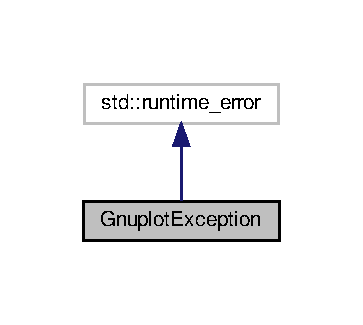
\includegraphics[width=174pt]{classGnuplotException__inherit__graph}
\end{center}
\end{figure}


Collaboration diagram for Gnuplot\+Exception\+:\nopagebreak
\begin{figure}[H]
\begin{center}
\leavevmode
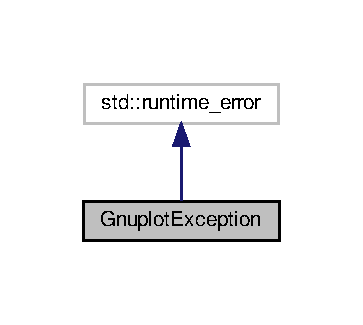
\includegraphics[width=174pt]{classGnuplotException__coll__graph}
\end{center}
\end{figure}
\subsection*{Public Member Functions}
\begin{DoxyCompactItemize}
\item 
\mbox{\Hypertarget{classGnuplotException_a8b324a9ef4d3f75079d41ecd61c62d44}\label{classGnuplotException_a8b324a9ef4d3f75079d41ecd61c62d44}} 
{\bfseries Gnuplot\+Exception} (const std\+::string \&msg)
\end{DoxyCompactItemize}


\subsection{Detailed Description}
A C++ interface to gnuplot. 

The interface uses pipes and so won\textquotesingle{}t run on a system that doesn\textquotesingle{}t have P\+O\+S\+IX pipe support Tested on Windows (Min\+GW and Visual C++) and Linux (G\+CC)

Version history\+: 0. C interface by N. Devillard (27/01/03)
\begin{DoxyEnumerate}
\item C++ interface\+: direct translation from the C interface by Rajarshi Guha (07/03/03)
\item corrections for Win32 compatibility by V. Chyzhdzenka (20/05/03)
\item some member functions added, corrections for Win32 and Linux compatibility by M. Burgis (10/03/08)
\end{DoxyEnumerate}

Requirements\+:
\begin{DoxyItemize}
\item gnuplot has to be installed (\href{http://www.gnuplot.info/download.html}{\tt http\+://www.\+gnuplot.\+info/download.\+html})
\item for Windows\+: set Path-\/\+Variable for \hyperlink{classGnuplot}{Gnuplot} path (e.\+g. C\+:/program files/gnuplot/bin) or set \hyperlink{classGnuplot}{Gnuplot} path with\+: \hyperlink{classGnuplot_a67cae885c26ced821e335d98986f1967}{Gnuplot\+::set\+\_\+\+G\+N\+U\+Plot\+Path(const std\+::string \&path)}; 
\end{DoxyItemize}

The documentation for this class was generated from the following file\+:\begin{DoxyCompactItemize}
\item 
gnuplot\+\_\+i.\+hpp\end{DoxyCompactItemize}

\hypertarget{structGPSCoordinates}{}\section{G\+P\+S\+Coordinates Struct Reference}
\label{structGPSCoordinates}\index{G\+P\+S\+Coordinates@{G\+P\+S\+Coordinates}}


A structure which saves the G\+PS coordinates.  




{\ttfamily \#include $<$Antenna\+Positioning.\+h$>$}

\subsection*{Public Attributes}
\begin{DoxyCompactItemize}
\item 
\mbox{\Hypertarget{structGPSCoordinates_ab4a3d3e2b7e7f5d13a4fe0779ccc2724}\label{structGPSCoordinates_ab4a3d3e2b7e7f5d13a4fe0779ccc2724}} 
double \hyperlink{structGPSCoordinates_ab4a3d3e2b7e7f5d13a4fe0779ccc2724}{latitude}
\begin{DoxyCompactList}\small\item\em Both quantities are in decimal degrees and they are negatives in western and southern hemispheres. \end{DoxyCompactList}\item 
\mbox{\Hypertarget{structGPSCoordinates_a1696c867f5a1d459e7a5ea11f43c3f9e}\label{structGPSCoordinates_a1696c867f5a1d459e7a5ea11f43c3f9e}} 
double {\bfseries longitude}
\end{DoxyCompactItemize}


\subsection{Detailed Description}
A structure which saves the G\+PS coordinates. 

The documentation for this struct was generated from the following file\+:\begin{DoxyCompactItemize}
\item 
\hyperlink{AntennaPositioning_8h}{Antenna\+Positioning.\+h}\end{DoxyCompactItemize}

\hypertarget{classGPSInterface}{}\section{G\+P\+S\+Interface Class Reference}
\label{classGPSInterface}\index{G\+P\+S\+Interface@{G\+P\+S\+Interface}}


It is intended to establish the communication with the Aaronia G\+PS receiver, to request and capture messages from this and extract useful data from messages.  




{\ttfamily \#include $<$Antenna\+Positioning.\+h$>$}

\subsection*{Public Member Functions}
\begin{DoxyCompactItemize}
\item 
\hyperlink{classGPSInterface_a91c9f19d6588bcd34a8038bdc036c20c}{G\+P\+S\+Interface} ()
\begin{DoxyCompactList}\small\item\em The default constructor of class \hyperlink{classGPSInterface}{G\+P\+S\+Interface}. \end{DoxyCompactList}\item 
\hyperlink{classGPSInterface_ac8156be0348867ab39ba6e7909e16c3b}{$\sim$\+G\+P\+S\+Interface} ()
\begin{DoxyCompactList}\small\item\em The \hyperlink{classGPSInterface}{G\+P\+S\+Interface} class\textquotesingle{} destructor. \end{DoxyCompactList}\item 
void \hyperlink{classGPSInterface_ac4a2712c98235f5ca2d826525180840b}{Initialize} ()
\begin{DoxyCompactList}\small\item\em This method is intended to try the communication with the Aaronia G\+PS receiver and configure this. \end{DoxyCompactList}\item 
\mbox{\Hypertarget{classGPSInterface_a3f92ed959a1ea60258e48ca7c379aec1}\label{classGPSInterface_a3f92ed959a1ea60258e48ca7c379aec1}} 
unsigned int \hyperlink{classGPSInterface_a3f92ed959a1ea60258e48ca7c379aec1}{Available} ()
\begin{DoxyCompactList}\small\item\em This method return the number of bytes in the input buffer, using the function F\+T\+\_\+\+Get\+Queue\+Status() of the D2\+XX library. \end{DoxyCompactList}\item 
\mbox{\Hypertarget{classGPSInterface_acfbd1398a99916c1009b0ac00098ca67}\label{classGPSInterface_acfbd1398a99916c1009b0ac00098ca67}} 
void \hyperlink{classGPSInterface_acfbd1398a99916c1009b0ac00098ca67}{Read\+One\+Data\+Set} ()
\begin{DoxyCompactList}\small\item\em This method send a command to get just one data set, rather than a streaming of measurements, and update the class attributes with that data set. \end{DoxyCompactList}\item 
void \hyperlink{classGPSInterface_a663c36374cc097040cb8945a3c25b190}{Disable\+Streaming} ()
\begin{DoxyCompactList}\small\item\em This method is intended to disable the data streaming from the Aaronia G\+PS receiver. \end{DoxyCompactList}\item 
\mbox{\Hypertarget{classGPSInterface_a698c9b38eaaa36fef1abcbc19614e2ad}\label{classGPSInterface_a698c9b38eaaa36fef1abcbc19614e2ad}} 
void \hyperlink{classGPSInterface_a698c9b38eaaa36fef1abcbc19614e2ad}{Purge} ()
\begin{DoxyCompactList}\small\item\em A method intended to purge the input and output buffers of the U\+SB interface. \end{DoxyCompactList}\item 
\mbox{\Hypertarget{classGPSInterface_a6ca2cb996a9ed3c6cd436491c56aab18}\label{classGPSInterface_a6ca2cb996a9ed3c6cd436491c56aab18}} 
const \hyperlink{structTimeData}{Time\+Data} \& {\bfseries Get\+Time\+Data} () const
\item 
\mbox{\Hypertarget{classGPSInterface_a9c827a6ce3078c5e748105019b75e0e0}\label{classGPSInterface_a9c827a6ce3078c5e748105019b75e0e0}} 
const \hyperlink{structGPSCoordinates}{G\+P\+S\+Coordinates} \& {\bfseries Get\+Coordinates} () const
\item 
\mbox{\Hypertarget{classGPSInterface_ab07cafce284ff50540a2be5b00410e34}\label{classGPSInterface_ab07cafce284ff50540a2be5b00410e34}} 
unsigned int {\bfseries Get\+Num\+Of\+Satellites} () const
\item 
\mbox{\Hypertarget{classGPSInterface_ac70e16c9a95f440bc8ff58429b0db42a}\label{classGPSInterface_ac70e16c9a95f440bc8ff58429b0db42a}} 
float {\bfseries Get\+G\+P\+S\+Elevation} () const
\item 
\mbox{\Hypertarget{classGPSInterface_ac3672cc76506fe6ed1ee4824a57c0857}\label{classGPSInterface_ac3672cc76506fe6ed1ee4824a57c0857}} 
const \hyperlink{structData3D}{Data3D} \& {\bfseries Get\+Gyro\+Data} () const
\item 
\mbox{\Hypertarget{classGPSInterface_aa0032f67cd64db9ddeee1b275025b417}\label{classGPSInterface_aa0032f67cd64db9ddeee1b275025b417}} 
const \hyperlink{structData3D}{Data3D} \& {\bfseries Get\+Compass\+Data} () const
\item 
\mbox{\Hypertarget{classGPSInterface_a675644b668df300d19afaefff9849886}\label{classGPSInterface_a675644b668df300d19afaefff9849886}} 
const \hyperlink{structData3D}{Data3D} \& {\bfseries Get\+Acceler\+Data} () const
\item 
\mbox{\Hypertarget{classGPSInterface_a63ed7a32797c2fc7557bfdfdb74c43ed}\label{classGPSInterface_a63ed7a32797c2fc7557bfdfdb74c43ed}} 
float {\bfseries Get\+Pressure} () const
\item 
\mbox{\Hypertarget{classGPSInterface_ae6a0d54023d9b3be7ea8180e2a26a193}\label{classGPSInterface_ae6a0d54023d9b3be7ea8180e2a26a193}} 
float {\bfseries Get\+Pressure\+Elevation} () const
\item 
\mbox{\Hypertarget{classGPSInterface_a5443691a26eb05587190cf631ffbcec3}\label{classGPSInterface_a5443691a26eb05587190cf631ffbcec3}} 
double {\bfseries Get\+Yaw} () const
\item 
\mbox{\Hypertarget{classGPSInterface_a5cb902ccc2165294b4dacc7f660dcb5a}\label{classGPSInterface_a5cb902ccc2165294b4dacc7f660dcb5a}} 
double {\bfseries Get\+Roll} () const
\item 
\mbox{\Hypertarget{classGPSInterface_a27f5655d78068177d901933528f3ac6f}\label{classGPSInterface_a27f5655d78068177d901933528f3ac6f}} 
double {\bfseries Get\+Pitch} () const
\item 
\mbox{\Hypertarget{classGPSInterface_a568715247cbcfa261d68a030df7bd1ef}\label{classGPSInterface_a568715247cbcfa261d68a030df7bd1ef}} 
bool {\bfseries Is\+Connected} () const
\end{DoxyCompactItemize}


\subsection{Detailed Description}
It is intended to establish the communication with the Aaronia G\+PS receiver, to request and capture messages from this and extract useful data from messages. 

\subsection{Constructor \& Destructor Documentation}
\mbox{\Hypertarget{classGPSInterface_a91c9f19d6588bcd34a8038bdc036c20c}\label{classGPSInterface_a91c9f19d6588bcd34a8038bdc036c20c}} 
\index{G\+P\+S\+Interface@{G\+P\+S\+Interface}!G\+P\+S\+Interface@{G\+P\+S\+Interface}}
\index{G\+P\+S\+Interface@{G\+P\+S\+Interface}!G\+P\+S\+Interface@{G\+P\+S\+Interface}}
\subsubsection{\texorpdfstring{G\+P\+S\+Interface()}{GPSInterface()}}
{\footnotesize\ttfamily G\+P\+S\+Interface\+::\+G\+P\+S\+Interface (\begin{DoxyParamCaption}{ }\end{DoxyParamCaption})}



The default constructor of class \hyperlink{classGPSInterface}{G\+P\+S\+Interface}. 

The constructor has to include the custom V\+ID and P\+ID combination of Aaronia G\+PS receiver within the allowed combinations, then it has to open the communication with the G\+PS receiver and set up the U\+A\+RT port on the F\+T\+DI chip. \mbox{\Hypertarget{classGPSInterface_ac8156be0348867ab39ba6e7909e16c3b}\label{classGPSInterface_ac8156be0348867ab39ba6e7909e16c3b}} 
\index{G\+P\+S\+Interface@{G\+P\+S\+Interface}!````~G\+P\+S\+Interface@{$\sim$\+G\+P\+S\+Interface}}
\index{````~G\+P\+S\+Interface@{$\sim$\+G\+P\+S\+Interface}!G\+P\+S\+Interface@{G\+P\+S\+Interface}}
\subsubsection{\texorpdfstring{$\sim$\+G\+P\+S\+Interface()}{~GPSInterface()}}
{\footnotesize\ttfamily G\+P\+S\+Interface\+::$\sim$\+G\+P\+S\+Interface (\begin{DoxyParamCaption}{ }\end{DoxyParamCaption})}



The \hyperlink{classGPSInterface}{G\+P\+S\+Interface} class\textquotesingle{} destructor. 

The destructor has to make sure that the data streaming and the data logging into the micro\+SD card are stopped, and then it must close the communication with the Aaronia G\+PS receiver. 

\subsection{Member Function Documentation}
\mbox{\Hypertarget{classGPSInterface_a663c36374cc097040cb8945a3c25b190}\label{classGPSInterface_a663c36374cc097040cb8945a3c25b190}} 
\index{G\+P\+S\+Interface@{G\+P\+S\+Interface}!Disable\+Streaming@{Disable\+Streaming}}
\index{Disable\+Streaming@{Disable\+Streaming}!G\+P\+S\+Interface@{G\+P\+S\+Interface}}
\subsubsection{\texorpdfstring{Disable\+Streaming()}{DisableStreaming()}}
{\footnotesize\ttfamily void G\+P\+S\+Interface\+::\+Disable\+Streaming (\begin{DoxyParamCaption}{ }\end{DoxyParamCaption})}



This method is intended to disable the data streaming from the Aaronia G\+PS receiver. 

! This method is intended to enable the streaming of data from the G\+PS receiver. $\ast$! After the streaming has been enable the method Capture\+Stream\+Data() must be used to get the stream data ! This method is intended to capture the continuous flow of data (stream) which sent from the Aaronia G\+PS receiver (when the streming is enabled). $\ast$! When this method is called the G\+PS interface reads one set of data from the U\+SB interface and calls the method \mbox{\Hypertarget{classGPSInterface_ac4a2712c98235f5ca2d826525180840b}\label{classGPSInterface_ac4a2712c98235f5ca2d826525180840b}} 
\index{G\+P\+S\+Interface@{G\+P\+S\+Interface}!Initialize@{Initialize}}
\index{Initialize@{Initialize}!G\+P\+S\+Interface@{G\+P\+S\+Interface}}
\subsubsection{\texorpdfstring{Initialize()}{Initialize()}}
{\footnotesize\ttfamily void G\+P\+S\+Interface\+::\+Initialize (\begin{DoxyParamCaption}{ }\end{DoxyParamCaption})}



This method is intended to try the communication with the Aaronia G\+PS receiver and configure this. 

First, this method tries the communication with an ID command, and if the reply is right it shows the hardware version, firmware version and protocol version and then it disables the data streaming and the data logging into the micro\+SD card. After, the G\+PS interface set up the following variables\+: data rate of streaming, accelerometer range and bandwidth of the average filter of the gyroscope sensor. 

The documentation for this class was generated from the following files\+:\begin{DoxyCompactItemize}
\item 
\hyperlink{AntennaPositioning_8h}{Antenna\+Positioning.\+h}\item 
G\+P\+S\+Interface.\+cpp\end{DoxyCompactItemize}

\hypertarget{classReply}{}\section{Reply Class Reference}
\label{classReply}\index{Reply@{Reply}}


The class {\itshape \hyperlink{classReply}{Reply}} is intended to receive a bytes vector sent by the spectrum analyzer and to extract its information.  




{\ttfamily \#include $<$Spectran.\+h$>$}



Inheritance diagram for Reply\+:\nopagebreak
\begin{figure}[H]
\begin{center}
\leavevmode
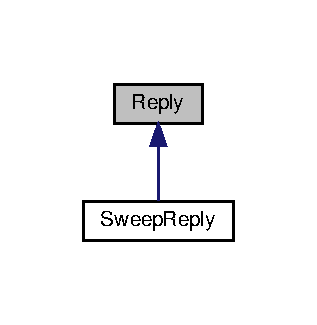
\includegraphics[width=152pt]{classReply__inherit__graph}
\end{center}
\end{figure}
\subsection*{Public Types}
\begin{DoxyCompactItemize}
\item 
enum \hyperlink{classReply_aa873dec4817ed08a5212ec3ba2b5c807}{Reply\+Type} \+: char \{ \newline
{\bfseries V\+E\+R\+I\+FY} =0x01, 
{\bfseries G\+E\+T\+S\+T\+P\+V\+AR} =0x20, 
{\bfseries S\+E\+T\+S\+T\+P\+V\+AR}, 
{\bfseries A\+M\+P\+F\+R\+E\+Q\+D\+AT}, 
\newline
{\bfseries U\+N\+I\+N\+I\+T\+I\+A\+L\+I\+Z\+ED}
 \}\begin{DoxyCompactList}\small\item\em An enumeration which contains the reply types which can be received from a Spectran H\+F-\/60105 V4 X spectrum analyzer. \end{DoxyCompactList}
\end{DoxyCompactItemize}
\subsection*{Public Member Functions}
\begin{DoxyCompactItemize}
\item 
\mbox{\Hypertarget{classReply_a48042b6ebf852fd8f0c28664eadf851e}\label{classReply_a48042b6ebf852fd8f0c28664eadf851e}} 
\hyperlink{classReply_a48042b6ebf852fd8f0c28664eadf851e}{Reply} ()
\begin{DoxyCompactList}\small\item\em The default constructor. \end{DoxyCompactList}\item 
\hyperlink{classReply_a4c993ea22d3674d2a337b6ca157d2bea}{Reply} (const \hyperlink{classReply_aa873dec4817ed08a5212ec3ba2b5c807}{Reply\+Type} type, const \hyperlink{Spectran_8h_a0411392c90f0c8f0d8e44a4e94259276}{Spec\+Variable} variable=Spec\+Variable\+::\+U\+N\+I\+N\+I\+T\+I\+A\+L\+I\+Z\+ED)
\begin{DoxyCompactList}\small\item\em A constructor which allows to set the reply type and the variable name, in case of {\itshape G\+E\+T\+S\+T\+P\+V\+AR} replies, and prepare the object to receive a spectrum analyzer\textquotesingle{}s reply. \end{DoxyCompactList}\item 
\hyperlink{classReply_add752285090cf6966ba993aae7056229}{Reply} (const \hyperlink{classReply}{Reply} \&another\+Reply)
\begin{DoxyCompactList}\small\item\em The copy constructor. \end{DoxyCompactList}\item 
virtual \hyperlink{classReply_a165e19cb7b393c0993d8992d47e7141d}{$\sim$\+Reply} ()
\begin{DoxyCompactList}\small\item\em The class destructor which is defined as virtual because there are some classes derived from this one. \end{DoxyCompactList}\item 
virtual void \hyperlink{classReply_a8c27c3e783dcc1ce75f709114b7e79f1}{Prepare\+To} (const \hyperlink{classReply_aa873dec4817ed08a5212ec3ba2b5c807}{Reply\+Type} type, const \hyperlink{Spectran_8h_a0411392c90f0c8f0d8e44a4e94259276}{Spec\+Variable} variable=Spec\+Variable\+::\+U\+N\+I\+N\+I\+T\+I\+A\+L\+I\+Z\+ED)
\begin{DoxyCompactList}\small\item\em This method is intended to set the reply type and variable name, in case of {\itshape G\+E\+T\+S\+T\+P\+V\+AR} replies, and to ask the object to prepare itself to receive the bytes. \end{DoxyCompactList}\item 
virtual void \hyperlink{classReply_a005fb1894b469cc16e69bf93fed967af}{Insert\+Bytes} (const std\+::uint8\+\_\+t $\ast$data)
\begin{DoxyCompactList}\small\item\em This method is intended to insert a reply\textquotesingle{}s bytes and to extract its data. \end{DoxyCompactList}\item 
\mbox{\Hypertarget{classReply_ab9eca743c910c467007488cdbb8125b8}\label{classReply_ab9eca743c910c467007488cdbb8125b8}} 
\hyperlink{classReply_aa873dec4817ed08a5212ec3ba2b5c807}{Reply\+Type} \hyperlink{classReply_ab9eca743c910c467007488cdbb8125b8}{Get\+Reply\+Type} () const
\begin{DoxyCompactList}\small\item\em This method returns the reply type as the corresponding value of the enumeration {\itshape Reply\+Type}. \end{DoxyCompactList}\item 
\mbox{\Hypertarget{classReply_a72a6fd5b94e9842916f55b3420e8b05f}\label{classReply_a72a6fd5b94e9842916f55b3420e8b05f}} 
std\+::string \hyperlink{classReply_a72a6fd5b94e9842916f55b3420e8b05f}{Get\+Reply\+Type\+String} () const
\begin{DoxyCompactList}\small\item\em A method which returns the reply type as a {\ttfamily std\+::string}. \end{DoxyCompactList}\item 
\mbox{\Hypertarget{classReply_adb2d432c7d1dbe6bddd4b6900eeea7e3}\label{classReply_adb2d432c7d1dbe6bddd4b6900eeea7e3}} 
std\+::string \hyperlink{classReply_adb2d432c7d1dbe6bddd4b6900eeea7e3}{Get\+Variable\+Name\+String} () const
\begin{DoxyCompactList}\small\item\em A method which returns the name of the Spectran\textquotesingle{}s variable which is related with the reply (G\+E\+T\+S\+T\+P\+V\+AR reply) as a {\ttfamily std\+::string}. \end{DoxyCompactList}\item 
\mbox{\Hypertarget{classReply_a027a08e481d00901d55bf7cfd5e7eb5f}\label{classReply_a027a08e481d00901d55bf7cfd5e7eb5f}} 
const std\+::vector$<$ std\+::uint8\+\_\+t $>$ \& \hyperlink{classReply_a027a08e481d00901d55bf7cfd5e7eb5f}{Get\+Bytes\+Vector} () const
\begin{DoxyCompactList}\small\item\em A method to get the bytes vector like this is implemented internally, a {\ttfamily std\+::vector} container. \end{DoxyCompactList}\item 
\mbox{\Hypertarget{classReply_a69d6dc14661b2a2148d16a1345cebc32}\label{classReply_a69d6dc14661b2a2148d16a1345cebc32}} 
const std\+::uint8\+\_\+t $\ast$ \hyperlink{classReply_a69d6dc14661b2a2148d16a1345cebc32}{Get\+Bytes\+Pointer} () const
\begin{DoxyCompactList}\small\item\em A method to get a direct pointer to the bytes of the internal vector. \end{DoxyCompactList}\item 
\mbox{\Hypertarget{classReply_a8aada6cea6e2008c6ba824fc7035627f}\label{classReply_a8aada6cea6e2008c6ba824fc7035627f}} 
unsigned int \hyperlink{classReply_a8aada6cea6e2008c6ba824fc7035627f}{Get\+Num\+Of\+Bytes} () const
\begin{DoxyCompactList}\small\item\em A method which allows to know the size of the bytes vector. \end{DoxyCompactList}\item 
\mbox{\Hypertarget{classReply_a4d9caba2f778fc50ea55e937f01e16db}\label{classReply_a4d9caba2f778fc50ea55e937f01e16db}} 
float \hyperlink{classReply_a4d9caba2f778fc50ea55e937f01e16db}{Get\+Value} () const
\begin{DoxyCompactList}\small\item\em A method to get the value of the variable which was queried with a {\itshape G\+E\+T\+S\+T\+P\+V\+AR} command or a power value (or voltage or field strength) which was received with a {\itshape A\+M\+P\+F\+R\+E\+Q\+D\+AT} reply. \end{DoxyCompactList}\item 
bool \hyperlink{classReply_a8527429859aeab3a0e62081871e5ce92}{Is\+Right} () const
\begin{DoxyCompactList}\small\item\em This method states if the received reply is right. \end{DoxyCompactList}\item 
\mbox{\Hypertarget{classReply_a387ea6ba4bad8ad832c2e5f4a95878d6}\label{classReply_a387ea6ba4bad8ad832c2e5f4a95878d6}} 
virtual void \hyperlink{classReply_a387ea6ba4bad8ad832c2e5f4a95878d6}{Clear} ()
\begin{DoxyCompactList}\small\item\em This method resets the object. \end{DoxyCompactList}\item 
virtual const \hyperlink{classReply}{Reply} \& \hyperlink{classReply_a7a4a6c76ee53d9ecf9833ab2880c3420}{operator=} (const \hyperlink{classReply}{Reply} \&another\+Reply)
\begin{DoxyCompactList}\small\item\em An overloading of the assignment operator, adapted to this class. \end{DoxyCompactList}\end{DoxyCompactItemize}
\subsection*{Protected Member Functions}
\begin{DoxyCompactItemize}
\item 
void \hyperlink{classReply_a8a6a68aeda60bfda6615272d2905a1ac}{Fill\+Bytes\+Vector} (const std\+::uint8\+\_\+t $\ast$data)
\begin{DoxyCompactList}\small\item\em This method fills correctly the internal bytes vector with the received bytes. \end{DoxyCompactList}\end{DoxyCompactItemize}
\subsection*{Protected Attributes}
\begin{DoxyCompactItemize}
\item 
\mbox{\Hypertarget{classReply_af9a348b823fc5ef09b470ba2cf2f625a}\label{classReply_af9a348b823fc5ef09b470ba2cf2f625a}} 
std\+::vector$<$ std\+::uint8\+\_\+t $>$ \hyperlink{classReply_af9a348b823fc5ef09b470ba2cf2f625a}{bytes}
\begin{DoxyCompactList}\small\item\em Bytes array (or vector) which has been received from the spectrum analyzer. \end{DoxyCompactList}\item 
\mbox{\Hypertarget{classReply_ae6d1cce2fdfa549568ad0ec9f5c6f13c}\label{classReply_ae6d1cce2fdfa549568ad0ec9f5c6f13c}} 
float \hyperlink{classReply_ae6d1cce2fdfa549568ad0ec9f5c6f13c}{value}
\begin{DoxyCompactList}\small\item\em The value (as a floating-\/point number) of a queried Spectran variable or a power value (or voltage of field strength). It has sense with {\itshape G\+E\+T\+S\+T\+P\+V\+AR} and {\itshape A\+M\+P\+F\+R\+E\+Q\+D\+AT} replies. \end{DoxyCompactList}\end{DoxyCompactItemize}


\subsection{Detailed Description}
The class {\itshape \hyperlink{classReply}{Reply}} is intended to receive a bytes vector sent by the spectrum analyzer and to extract its information. 

When a command is sent to a Spectran H\+F-\/60105 V4 X spectrum analyzer, this will respond with another bytes vector (however some commands do not have reply), so the idea is to insert this in an object of class {\itshape \hyperlink{classReply}{Reply}}, then the object will process and extract the info (variable id, value, etc.) of the bytes vector and finally the info will be available through the \char`\"{}\+Get\char`\"{} methods. 

\subsection{Member Enumeration Documentation}
\mbox{\Hypertarget{classReply_aa873dec4817ed08a5212ec3ba2b5c807}\label{classReply_aa873dec4817ed08a5212ec3ba2b5c807}} 
\index{Reply@{Reply}!Reply\+Type@{Reply\+Type}}
\index{Reply\+Type@{Reply\+Type}!Reply@{Reply}}
\subsubsection{\texorpdfstring{Reply\+Type}{ReplyType}}
{\footnotesize\ttfamily enum \hyperlink{classReply_aa873dec4817ed08a5212ec3ba2b5c807}{Reply\+::\+Reply\+Type} \+: char}



An enumeration which contains the reply types which can be received from a Spectran H\+F-\/60105 V4 X spectrum analyzer. 

This enumeration contains just four replies from the Spectran U\+SB Protocol\+: {\itshape V\+E\+R\+I\+FY}, {\itshape G\+E\+T\+S\+T\+P\+V\+AR}, {\itshape S\+E\+T\+S\+T\+P\+V\+AR} and {\itshape A\+M\+P\+F\+R\+E\+Q\+D\+AT}. The other replies are received when an internal file of the spectrum analyzer have been queried or modified, and because that will not be done, they are not added. There is an extra command type which is {\itshape U\+N\+I\+N\+I\+T\+I\+A\+L\+I\+Z\+ED} whose purpose is to state that the object is not prepared. 

\subsection{Constructor \& Destructor Documentation}
\mbox{\Hypertarget{classReply_a4c993ea22d3674d2a337b6ca157d2bea}\label{classReply_a4c993ea22d3674d2a337b6ca157d2bea}} 
\index{Reply@{Reply}!Reply@{Reply}}
\index{Reply@{Reply}!Reply@{Reply}}
\subsubsection{\texorpdfstring{Reply()}{Reply()}\hspace{0.1cm}{\footnotesize\ttfamily [1/2]}}
{\footnotesize\ttfamily Reply\+::\+Reply (\begin{DoxyParamCaption}\item[{const \hyperlink{classReply_aa873dec4817ed08a5212ec3ba2b5c807}{Reply\+Type}}]{type,  }\item[{const \hyperlink{Spectran_8h_a0411392c90f0c8f0d8e44a4e94259276}{Spec\+Variable}}]{variable = {\ttfamily SpecVariable\+:\+:UNINITIALIZED} }\end{DoxyParamCaption})}



A constructor which allows to set the reply type and the variable name, in case of {\itshape G\+E\+T\+S\+T\+P\+V\+AR} replies, and prepare the object to receive a spectrum analyzer\textquotesingle{}s reply. 


\begin{DoxyParams}[1]{Parameters}
\mbox{\tt in}  & {\em type} & The reply type\+: V\+E\+R\+I\+FY, G\+E\+T\+S\+T\+P\+V\+AR, S\+E\+T\+S\+T\+P\+V\+AR or A\+M\+P\+F\+R\+E\+Q\+D\+AT. \\
\hline
\mbox{\tt in}  & {\em variable} & An optional argument which indicates the variable whose value will be received by a G\+E\+T\+S\+T\+P\+V\+AR reply. \\
\hline
\end{DoxyParams}
\mbox{\Hypertarget{classReply_add752285090cf6966ba993aae7056229}\label{classReply_add752285090cf6966ba993aae7056229}} 
\index{Reply@{Reply}!Reply@{Reply}}
\index{Reply@{Reply}!Reply@{Reply}}
\subsubsection{\texorpdfstring{Reply()}{Reply()}\hspace{0.1cm}{\footnotesize\ttfamily [2/2]}}
{\footnotesize\ttfamily Reply\+::\+Reply (\begin{DoxyParamCaption}\item[{const \hyperlink{classReply}{Reply} \&}]{another\+Reply }\end{DoxyParamCaption})}



The copy constructor. 


\begin{DoxyParams}[1]{Parameters}
\mbox{\tt in}  & {\em another\+Reply} & A {\itshape \hyperlink{classReply}{Reply}} object which is given to copy its attributes. \\
\hline
\end{DoxyParams}
\mbox{\Hypertarget{classReply_a165e19cb7b393c0993d8992d47e7141d}\label{classReply_a165e19cb7b393c0993d8992d47e7141d}} 
\index{Reply@{Reply}!````~Reply@{$\sim$\+Reply}}
\index{````~Reply@{$\sim$\+Reply}!Reply@{Reply}}
\subsubsection{\texorpdfstring{$\sim$\+Reply()}{~Reply()}}
{\footnotesize\ttfamily virtual Reply\+::$\sim$\+Reply (\begin{DoxyParamCaption}{ }\end{DoxyParamCaption})\hspace{0.3cm}{\ttfamily [inline]}, {\ttfamily [virtual]}}



The class destructor which is defined as virtual because there are some classes derived from this one. 

It was necessary to implement the destructor here to define this one as {\itshape virtual}. However, it was not necessary to explicitly clean, close and/or destroy any attribute and, because of that, the implementation is empty. 

\subsection{Member Function Documentation}
\mbox{\Hypertarget{classReply_a8a6a68aeda60bfda6615272d2905a1ac}\label{classReply_a8a6a68aeda60bfda6615272d2905a1ac}} 
\index{Reply@{Reply}!Fill\+Bytes\+Vector@{Fill\+Bytes\+Vector}}
\index{Fill\+Bytes\+Vector@{Fill\+Bytes\+Vector}!Reply@{Reply}}
\subsubsection{\texorpdfstring{Fill\+Bytes\+Vector()}{FillBytesVector()}}
{\footnotesize\ttfamily void Reply\+::\+Fill\+Bytes\+Vector (\begin{DoxyParamCaption}\item[{const std\+::uint8\+\_\+t $\ast$}]{data }\end{DoxyParamCaption})\hspace{0.3cm}{\ttfamily [protected]}}



This method fills correctly the internal bytes vector with the received bytes. 


\begin{DoxyParams}[1]{Parameters}
\mbox{\tt in}  & {\em data} & A pointer to the bytes which contain the information of the reply sent by the spectrum analyzer. \\
\hline
\end{DoxyParams}
\mbox{\Hypertarget{classReply_a005fb1894b469cc16e69bf93fed967af}\label{classReply_a005fb1894b469cc16e69bf93fed967af}} 
\index{Reply@{Reply}!Insert\+Bytes@{Insert\+Bytes}}
\index{Insert\+Bytes@{Insert\+Bytes}!Reply@{Reply}}
\subsubsection{\texorpdfstring{Insert\+Bytes()}{InsertBytes()}}
{\footnotesize\ttfamily void Reply\+::\+Insert\+Bytes (\begin{DoxyParamCaption}\item[{const std\+::uint8\+\_\+t $\ast$}]{data }\end{DoxyParamCaption})\hspace{0.3cm}{\ttfamily [virtual]}}



This method is intended to insert a reply\textquotesingle{}s bytes and to extract its data. 

The reply object must have been prepared before inserting the bytes vector. 
\begin{DoxyParams}[1]{Parameters}
\mbox{\tt in}  & {\em data} & A pointer to the bytes which must be inserted in the object and from which the info must be extracted. \\
\hline
\end{DoxyParams}


Reimplemented in \hyperlink{classSweepReply_a8eff11f046d6cd2fb8c3987f889c5d11}{Sweep\+Reply}.

\mbox{\Hypertarget{classReply_a8527429859aeab3a0e62081871e5ce92}\label{classReply_a8527429859aeab3a0e62081871e5ce92}} 
\index{Reply@{Reply}!Is\+Right@{Is\+Right}}
\index{Is\+Right@{Is\+Right}!Reply@{Reply}}
\subsubsection{\texorpdfstring{Is\+Right()}{IsRight()}}
{\footnotesize\ttfamily bool Reply\+::\+Is\+Right (\begin{DoxyParamCaption}{ }\end{DoxyParamCaption}) const}



This method states if the received reply is right. 

To do so, the method checks if the reply type (determined when the reply object was prepared) is equal to first received byte and if the reply type is V\+E\+R\+I\+FY it checks if the following bytes are correct, or if the reply type is G\+E\+T\+S\+T\+P\+V\+AR or S\+E\+T\+S\+T\+P\+V\+AR it checks the \char`\"{}status\char`\"{} byte, which must be zero when all is right. By default the method indicates that the reply is incorrect. \mbox{\Hypertarget{classReply_a7a4a6c76ee53d9ecf9833ab2880c3420}\label{classReply_a7a4a6c76ee53d9ecf9833ab2880c3420}} 
\index{Reply@{Reply}!operator=@{operator=}}
\index{operator=@{operator=}!Reply@{Reply}}
\subsubsection{\texorpdfstring{operator=()}{operator=()}}
{\footnotesize\ttfamily const \hyperlink{classReply}{Reply} \& Reply\+::operator= (\begin{DoxyParamCaption}\item[{const \hyperlink{classReply}{Reply} \&}]{another\+Reply }\end{DoxyParamCaption})\hspace{0.3cm}{\ttfamily [virtual]}}



An overloading of the assignment operator, adapted to this class. 


\begin{DoxyParams}[1]{Parameters}
\mbox{\tt in}  & {\em another\+Reply} & A {\itshape \hyperlink{classReply}{Reply}} object which is given to copy its attributes. \\
\hline
\end{DoxyParams}
\mbox{\Hypertarget{classReply_a8c27c3e783dcc1ce75f709114b7e79f1}\label{classReply_a8c27c3e783dcc1ce75f709114b7e79f1}} 
\index{Reply@{Reply}!Prepare\+To@{Prepare\+To}}
\index{Prepare\+To@{Prepare\+To}!Reply@{Reply}}
\subsubsection{\texorpdfstring{Prepare\+To()}{PrepareTo()}}
{\footnotesize\ttfamily void Reply\+::\+Prepare\+To (\begin{DoxyParamCaption}\item[{const \hyperlink{classReply_aa873dec4817ed08a5212ec3ba2b5c807}{Reply\+Type}}]{type,  }\item[{const \hyperlink{Spectran_8h_a0411392c90f0c8f0d8e44a4e94259276}{Spec\+Variable}}]{variable = {\ttfamily SpecVariable\+:\+:UNINITIALIZED} }\end{DoxyParamCaption})\hspace{0.3cm}{\ttfamily [virtual]}}



This method is intended to set the reply type and variable name, in case of {\itshape G\+E\+T\+S\+T\+P\+V\+AR} replies, and to ask the object to prepare itself to receive the bytes. 

The tasks performed by this methods are\+: to clear the object, to set the reply type and then to call the private method {\ttfamily Prepare\+Reply()}. The variable name must be set for the G\+E\+T\+S\+T\+P\+V\+AR replies, for other cases it is not important. 
\begin{DoxyParams}[1]{Parameters}
\mbox{\tt in}  & {\em type} & The reply type\+: V\+E\+R\+I\+FY, G\+E\+T\+S\+T\+P\+V\+AR, S\+E\+T\+S\+T\+P\+V\+AR or A\+M\+P\+F\+R\+E\+Q\+D\+AT. \\
\hline
\mbox{\tt in}  & {\em variable} & An optional argument which indicates the variable whose value will be received by a G\+E\+T\+S\+T\+P\+V\+AR reply. \\
\hline
\end{DoxyParams}


Reimplemented in \hyperlink{classSweepReply_a513705c42bec154f66f75903813a5db1}{Sweep\+Reply}.



The documentation for this class was generated from the following files\+:\begin{DoxyCompactItemize}
\item 
\hyperlink{Spectran_8h}{Spectran.\+h}\item 
\hyperlink{Reply_8cpp}{Reply.\+cpp}\end{DoxyCompactItemize}

\hypertarget{structRFI}{}\section{R\+FI Struct Reference}
\label{structRFI}\index{R\+FI@{R\+FI}}


The aim of this structure is to store the data related with the detected RF interference (\hyperlink{structRFI}{R\+FI})\+: frequency, power, azimuth angle, polarization, time, reference norm, etc.  




{\ttfamily \#include $<$Basics.\+h$>$}



Inheritance diagram for R\+FI\+:\nopagebreak
\begin{figure}[H]
\begin{center}
\leavevmode
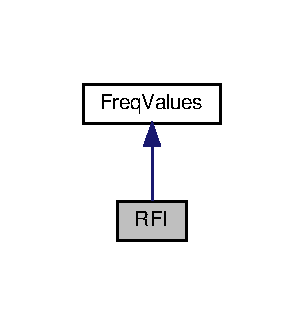
\includegraphics[width=146pt]{structRFI__inherit__graph}
\end{center}
\end{figure}


Collaboration diagram for R\+FI\+:\nopagebreak
\begin{figure}[H]
\begin{center}
\leavevmode
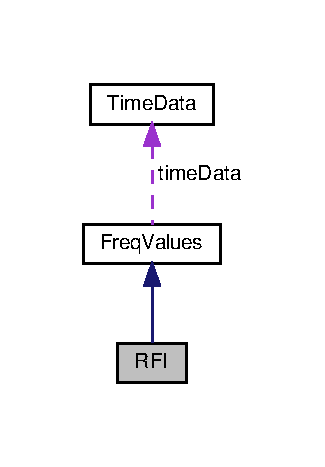
\includegraphics[width=156pt]{structRFI__coll__graph}
\end{center}
\end{figure}
\subsection*{Public Types}
\begin{DoxyCompactItemize}
\item 
\mbox{\Hypertarget{structRFI_a18cfa7d24274bbcd14acc6b513860cb0}\label{structRFI_a18cfa7d24274bbcd14acc6b513860cb0}} 
enum \hyperlink{structRFI_a18cfa7d24274bbcd14acc6b513860cb0}{Thresholds\+Norm} \{ {\bfseries I\+T\+U\+\_\+\+R\+A769\+\_\+2\+\_\+\+V\+L\+BI}, 
{\bfseries S\+K\+A\+\_\+\+M\+O\+D\+E1}, 
{\bfseries S\+K\+A\+\_\+\+M\+O\+D\+E2}
 \}\begin{DoxyCompactList}\small\item\em Enumeration which contains the reference documents (recommendations, protocols, etc.) of harmful \hyperlink{structRFI}{R\+FI} levels (a.\+k.\+a. thresholds)\+: the I\+TU recommendation R\+A.\+769-\/2, S\+KA protocol Mode 1, S\+KA protocol Mode 2. \end{DoxyCompactList}
\end{DoxyCompactItemize}
\subsection*{Public Member Functions}
\begin{DoxyCompactItemize}
\item 
\mbox{\Hypertarget{structRFI_ad0183cf1bc28c3f907e16428a5816e35}\label{structRFI_ad0183cf1bc28c3f907e16428a5816e35}} 
\hyperlink{structRFI_ad0183cf1bc28c3f907e16428a5816e35}{R\+FI} ()
\begin{DoxyCompactList}\small\item\em The default constructor which calls the default constructor of structure {\itshape \hyperlink{structFreqValues}{Freq\+Values}} and set type to \char`\"{}rfi\char`\"{}, azimuth angle to zero, number of bands to zero and set, by default, threshold norm to S\+K\+A\+\_\+\+M\+O\+D\+E1. \end{DoxyCompactList}\item 
\hyperlink{structRFI_a82852dbeab11484c90d4b339f63aefa9}{R\+FI} (const \hyperlink{structRFI}{R\+FI} \&rfi)
\begin{DoxyCompactList}\small\item\em The copy constructor which receives a {\itshape \hyperlink{structRFI}{R\+FI}} object. \end{DoxyCompactList}\item 
\mbox{\Hypertarget{structRFI_a103d0419053a7e323647cdafb3b036e3}\label{structRFI_a103d0419053a7e323647cdafb3b036e3}} 
void \hyperlink{structRFI_a103d0419053a7e323647cdafb3b036e3}{Clear} ()
\begin{DoxyCompactList}\small\item\em The aim of this method is to clean the attributes of this structure. \end{DoxyCompactList}\item 
const \hyperlink{structRFI}{R\+FI} \& \hyperlink{structRFI_a8fcc866a09f2f88a9754e04a1d056104}{operator=} (const \hyperlink{structRFI}{R\+FI} \&another\+R\+FI)
\begin{DoxyCompactList}\small\item\em An overloading of the assignment operator adapted to receive a {\itshape \hyperlink{structRFI}{R\+FI}} object. \end{DoxyCompactList}\end{DoxyCompactItemize}
\subsection*{Public Attributes}
\begin{DoxyCompactItemize}
\item 
\mbox{\Hypertarget{structRFI_aeb10ac61d7897dbaa6971607e56ea244}\label{structRFI_aeb10ac61d7897dbaa6971607e56ea244}} 
float \hyperlink{structRFI_aeb10ac61d7897dbaa6971607e56ea244}{azimuth\+Angle}
\begin{DoxyCompactList}\small\item\em The azimuth angle where this \hyperlink{structRFI}{R\+FI} was detected. \end{DoxyCompactList}\item 
\mbox{\Hypertarget{structRFI_a6c5345dd1141e8bf80b4e1cf32c092de}\label{structRFI_a6c5345dd1141e8bf80b4e1cf32c092de}} 
std\+::string \hyperlink{structRFI_a6c5345dd1141e8bf80b4e1cf32c092de}{polarization}
\begin{DoxyCompactList}\small\item\em The antenna polarization of the sweep where the \hyperlink{structRFI}{R\+FI} was detected. \end{DoxyCompactList}\item 
\mbox{\Hypertarget{structRFI_aefedd07c1a853fb1c8363a0f436d3973}\label{structRFI_aefedd07c1a853fb1c8363a0f436d3973}} 
unsigned int \hyperlink{structRFI_aefedd07c1a853fb1c8363a0f436d3973}{num\+Of\+R\+F\+I\+Bands}
\begin{DoxyCompactList}\small\item\em The number of \hyperlink{structRFI}{R\+FI} bands defined as intervals of continuous data points where it was detected \hyperlink{structRFI}{R\+FI}. \end{DoxyCompactList}\item 
\hyperlink{structRFI_a18cfa7d24274bbcd14acc6b513860cb0}{Thresholds\+Norm} \hyperlink{structRFI_a48905b3dcebf7127bd31315a21a24599}{thresh\+Norm}
\end{DoxyCompactItemize}


\subsection{Detailed Description}
The aim of this structure is to store the data related with the detected RF interference (\hyperlink{structRFI}{R\+FI})\+: frequency, power, azimuth angle, polarization, time, reference norm, etc. 

\subsection{Constructor \& Destructor Documentation}
\mbox{\Hypertarget{structRFI_a82852dbeab11484c90d4b339f63aefa9}\label{structRFI_a82852dbeab11484c90d4b339f63aefa9}} 
\index{R\+FI@{R\+FI}!R\+FI@{R\+FI}}
\index{R\+FI@{R\+FI}!R\+FI@{R\+FI}}
\subsubsection{\texorpdfstring{R\+F\+I()}{RFI()}}
{\footnotesize\ttfamily R\+F\+I\+::\+R\+FI (\begin{DoxyParamCaption}\item[{const \hyperlink{structRFI}{R\+FI} \&}]{rfi }\end{DoxyParamCaption})\hspace{0.3cm}{\ttfamily [inline]}}



The copy constructor which receives a {\itshape \hyperlink{structRFI}{R\+FI}} object. 


\begin{DoxyParams}[1]{Parameters}
\mbox{\tt in}  & {\em rfi} & A {\itshape \hyperlink{structRFI}{R\+FI}} structure given to copy its attributes. \\
\hline
\end{DoxyParams}


\subsection{Member Function Documentation}
\mbox{\Hypertarget{structRFI_a8fcc866a09f2f88a9754e04a1d056104}\label{structRFI_a8fcc866a09f2f88a9754e04a1d056104}} 
\index{R\+FI@{R\+FI}!operator=@{operator=}}
\index{operator=@{operator=}!R\+FI@{R\+FI}}
\subsubsection{\texorpdfstring{operator=()}{operator=()}}
{\footnotesize\ttfamily const \hyperlink{structRFI}{R\+FI}\& R\+F\+I\+::operator= (\begin{DoxyParamCaption}\item[{const \hyperlink{structRFI}{R\+FI} \&}]{another\+R\+FI }\end{DoxyParamCaption})\hspace{0.3cm}{\ttfamily [inline]}}



An overloading of the assignment operator adapted to receive a {\itshape \hyperlink{structRFI}{R\+FI}} object. 


\begin{DoxyParams}[1]{Parameters}
\mbox{\tt in}  & {\em another\+R\+FI} & Another {\itshape \hyperlink{structRFI}{R\+FI}} structure given to copy its attributes. \\
\hline
\end{DoxyParams}


\subsection{Member Data Documentation}
\mbox{\Hypertarget{structRFI_a48905b3dcebf7127bd31315a21a24599}\label{structRFI_a48905b3dcebf7127bd31315a21a24599}} 
\index{R\+FI@{R\+FI}!thresh\+Norm@{thresh\+Norm}}
\index{thresh\+Norm@{thresh\+Norm}!R\+FI@{R\+FI}}
\subsubsection{\texorpdfstring{thresh\+Norm}{threshNorm}}
{\footnotesize\ttfamily \hyperlink{structRFI_a18cfa7d24274bbcd14acc6b513860cb0}{Thresholds\+Norm} R\+F\+I\+::thresh\+Norm}

The norm (recommendation, protocol, etc.) which was used to define the harmful interference levels. 

The documentation for this struct was generated from the following file\+:\begin{DoxyCompactItemize}
\item 
/home/new-\/mauro/eclipse-\/cdt/workspace/\+R\+F\+I\+M\+S\+\_\+\+C\+A\+R\+T/src/\hyperlink{Basics_8h}{Basics.\+h}\end{DoxyCompactItemize}

\hypertarget{classRFIDetector}{}\section{R\+F\+I\+Detector Class Reference}
\label{classRFIDetector}\index{R\+F\+I\+Detector@{R\+F\+I\+Detector}}


The aim of this class is to compare each calibrated sweep with a threshold curve to determine where there is RF interference (\hyperlink{structRFI}{R\+FI}).  




{\ttfamily \#include $<$Sweep\+Processing.\+h$>$}

\subsection*{Public Member Functions}
\begin{DoxyCompactItemize}
\item 
\hyperlink{classRFIDetector_a1943c00a5ab657a24cdacaf2b0d550f1}{R\+F\+I\+Detector} (\hyperlink{classCurveAdjuster}{Curve\+Adjuster} \&adj)
\begin{DoxyCompactList}\small\item\em The unique class constructor. \end{DoxyCompactList}\item 
\hyperlink{classRFIDetector_a6445cd27f7b22459d8f1e3b67c323cf0}{$\sim$\+R\+F\+I\+Detector} ()
\begin{DoxyCompactList}\small\item\em The class destructor. \end{DoxyCompactList}\item 
\mbox{\Hypertarget{classRFIDetector_aea149c6aa9fa7db44616973b27863ebc}\label{classRFIDetector_aea149c6aa9fa7db44616973b27863ebc}} 
void \hyperlink{classRFIDetector_aea149c6aa9fa7db44616973b27863ebc}{Set\+Bands\+Parameters} (const std\+::vector$<$ \hyperlink{structBandParameters}{Band\+Parameters} $>$ \&bands\+Param)
\begin{DoxyCompactList}\small\item\em A method to insert a vector with the parameters of all frequency bands. \end{DoxyCompactList}\item 
void \hyperlink{classRFIDetector_a1eba12febd92bba77f658dfe664ea5c6}{Load\+Thresh\+Curve} (const \hyperlink{structRFI_a18cfa7d24274bbcd14acc6b513860cb0}{R\+F\+I\+::\+Thresholds\+Norm} thr\+Norm)
\begin{DoxyCompactList}\small\item\em This method loads a determined thresholds curve from the corresponding file. \end{DoxyCompactList}\item 
const \hyperlink{structRFI}{R\+FI} \& \hyperlink{classRFIDetector_a98bf817b6c6aee954e0f0056fb5e4360}{Detect\+R\+FI} (const \hyperlink{structSweep}{Sweep} \&sweep)
\begin{DoxyCompactList}\small\item\em This method detects \hyperlink{structRFI}{R\+FI} in a calibrated sweep. \end{DoxyCompactList}\item 
\mbox{\Hypertarget{classRFIDetector_a6e2c5fbdb76bc7b752fb0fec3bc4f41c}\label{classRFIDetector_a6e2c5fbdb76bc7b752fb0fec3bc4f41c}} 
const \hyperlink{structFreqValues}{Freq\+Values} \& \hyperlink{classRFIDetector_a6e2c5fbdb76bc7b752fb0fec3bc4f41c}{Get\+Thresh\+Curve} () const
\begin{DoxyCompactList}\small\item\em This method returns the threshold curve which has been loaded. \end{DoxyCompactList}\item 
\mbox{\Hypertarget{classRFIDetector_a053ba4f21411a8671ff0a38f2a18d393}\label{classRFIDetector_a053ba4f21411a8671ff0a38f2a18d393}} 
unsigned int \hyperlink{classRFIDetector_a053ba4f21411a8671ff0a38f2a18d393}{Get\+Num\+Of\+R\+F\+I\+Bands} () const
\begin{DoxyCompactList}\small\item\em This method returns the number of \hyperlink{structRFI}{R\+FI} bands which were detected in the last sweep. \end{DoxyCompactList}\item 
\mbox{\Hypertarget{classRFIDetector_ad50815b6e1004d2a6c15aef7deaca272}\label{classRFIDetector_ad50815b6e1004d2a6c15aef7deaca272}} 
const \hyperlink{structRFI}{R\+FI} \& \hyperlink{classRFIDetector_ad50815b6e1004d2a6c15aef7deaca272}{Get\+R\+FI} () const
\begin{DoxyCompactList}\small\item\em This method returns the last detected \hyperlink{structRFI}{R\+FI}. \end{DoxyCompactList}\end{DoxyCompactItemize}


\subsection{Detailed Description}
The aim of this class is to compare each calibrated sweep with a threshold curve to determine where there is RF interference (\hyperlink{structRFI}{R\+FI}). 

\subsection{Constructor \& Destructor Documentation}
\mbox{\Hypertarget{classRFIDetector_a1943c00a5ab657a24cdacaf2b0d550f1}\label{classRFIDetector_a1943c00a5ab657a24cdacaf2b0d550f1}} 
\index{R\+F\+I\+Detector@{R\+F\+I\+Detector}!R\+F\+I\+Detector@{R\+F\+I\+Detector}}
\index{R\+F\+I\+Detector@{R\+F\+I\+Detector}!R\+F\+I\+Detector@{R\+F\+I\+Detector}}
\subsubsection{\texorpdfstring{R\+F\+I\+Detector()}{RFIDetector()}}
{\footnotesize\ttfamily R\+F\+I\+Detector\+::\+R\+F\+I\+Detector (\begin{DoxyParamCaption}\item[{\hyperlink{classCurveAdjuster}{Curve\+Adjuster} \&}]{adj }\end{DoxyParamCaption})\hspace{0.3cm}{\ttfamily [inline]}}



The unique class constructor. 

At instantiation the programmer must provide a reference to a {\itshape \hyperlink{classCurveAdjuster}{Curve\+Adjuster}} object. 
\begin{DoxyParams}[1]{Parameters}
\mbox{\tt in}  & {\em adj} & A {\itshape \hyperlink{classCurveAdjuster}{Curve\+Adjuster}} object. \\
\hline
\end{DoxyParams}
\mbox{\Hypertarget{classRFIDetector_a6445cd27f7b22459d8f1e3b67c323cf0}\label{classRFIDetector_a6445cd27f7b22459d8f1e3b67c323cf0}} 
\index{R\+F\+I\+Detector@{R\+F\+I\+Detector}!````~R\+F\+I\+Detector@{$\sim$\+R\+F\+I\+Detector}}
\index{````~R\+F\+I\+Detector@{$\sim$\+R\+F\+I\+Detector}!R\+F\+I\+Detector@{R\+F\+I\+Detector}}
\subsubsection{\texorpdfstring{$\sim$\+R\+F\+I\+Detector()}{~RFIDetector()}}
{\footnotesize\ttfamily R\+F\+I\+Detector\+::$\sim$\+R\+F\+I\+Detector (\begin{DoxyParamCaption}{ }\end{DoxyParamCaption})\hspace{0.3cm}{\ttfamily [inline]}}



The class destructor. 

Its implementation is empty because the attributes destruction is implicitly. However, the destructor is defined here to allow this one to be called explicitly in any part of the code, what is used by the signals handler to destroy the objects when a signal to finish the execution of the software is received. 

\subsection{Member Function Documentation}
\mbox{\Hypertarget{classRFIDetector_a98bf817b6c6aee954e0f0056fb5e4360}\label{classRFIDetector_a98bf817b6c6aee954e0f0056fb5e4360}} 
\index{R\+F\+I\+Detector@{R\+F\+I\+Detector}!Detect\+R\+FI@{Detect\+R\+FI}}
\index{Detect\+R\+FI@{Detect\+R\+FI}!R\+F\+I\+Detector@{R\+F\+I\+Detector}}
\subsubsection{\texorpdfstring{Detect\+R\+F\+I()}{DetectRFI()}}
{\footnotesize\ttfamily const \hyperlink{structRFI}{R\+FI} \& R\+F\+I\+Detector\+::\+Detect\+R\+FI (\begin{DoxyParamCaption}\item[{const \hyperlink{structSweep}{Sweep} \&}]{sweep }\end{DoxyParamCaption})}



This method detects \hyperlink{structRFI}{R\+FI} in a calibrated sweep. 

The given sweep should have been calibrated before. 
\begin{DoxyParams}[1]{Parameters}
\mbox{\tt in}  & {\em sweep} & A calibrated sweep. \\
\hline
\end{DoxyParams}
\begin{DoxyReturn}{Returns}
A structure with the pairs of values (frequency,power) where it was detected \hyperlink{structRFI}{R\+FI}. 
\end{DoxyReturn}
\mbox{\Hypertarget{classRFIDetector_a1eba12febd92bba77f658dfe664ea5c6}\label{classRFIDetector_a1eba12febd92bba77f658dfe664ea5c6}} 
\index{R\+F\+I\+Detector@{R\+F\+I\+Detector}!Load\+Thresh\+Curve@{Load\+Thresh\+Curve}}
\index{Load\+Thresh\+Curve@{Load\+Thresh\+Curve}!R\+F\+I\+Detector@{R\+F\+I\+Detector}}
\subsubsection{\texorpdfstring{Load\+Thresh\+Curve()}{LoadThreshCurve()}}
{\footnotesize\ttfamily void R\+F\+I\+Detector\+::\+Load\+Thresh\+Curve (\begin{DoxyParamCaption}\item[{const \hyperlink{structRFI_a18cfa7d24274bbcd14acc6b513860cb0}{R\+F\+I\+::\+Thresholds\+Norm}}]{thr\+Norm }\end{DoxyParamCaption})}



This method loads a determined thresholds curve from the corresponding file. 

The threshold curve is loaded from one of the fileS in the path \hyperlink{Basics_8h_a0423f4cb393331ce0b9f6b3a43adcaae}{B\+A\+S\+E\+\_\+\+P\+A\+TH}/thresholds/. The argument determines which recommendation, protocol or norm must be taken as reference to determine the threshold curve to be used, i.\+e. to determine from which file load that curve. 
\begin{DoxyParams}[1]{Parameters}
\mbox{\tt in}  & {\em thr\+Norm} & The norm, recommendation or protocol that must be taken as reference. \\
\hline
\end{DoxyParams}


The documentation for this class was generated from the following files\+:\begin{DoxyCompactItemize}
\item 
/home/new-\/mauro/eclipse-\/cdt/workspace/\+R\+F\+I\+M\+S\+\_\+\+C\+A\+R\+T/src/\hyperlink{SweepProcessing_8h}{Sweep\+Processing.\+h}\item 
/home/new-\/mauro/eclipse-\/cdt/workspace/\+R\+F\+I\+M\+S\+\_\+\+C\+A\+R\+T/src/\hyperlink{RFIDetector_8cpp}{R\+F\+I\+Detector.\+cpp}\end{DoxyCompactItemize}

\hypertarget{classRFPloter}{}\section{R\+F\+Ploter Class Reference}
\label{classRFPloter}\index{R\+F\+Ploter@{R\+F\+Ploter}}


The class {\itshape \hyperlink{classRFPloter}{R\+F\+Ploter}} is intended to plot sweeps, RF interference (\hyperlink{structRFI}{R\+FI}) and any frequency curve.  




{\ttfamily \#include $<$Sweep\+Processing.\+h$>$}

\subsection*{Public Member Functions}
\begin{DoxyCompactItemize}
\item 
\hyperlink{classRFPloter_ab7b36c6de3e288b7ab88238b16a0816a}{R\+F\+Ploter} (const std\+::string \&titl=\char`\"{}\char`\"{})
\begin{DoxyCompactList}\small\item\em The unique {\itshape \hyperlink{classRFPloter}{R\+F\+Ploter}} constructor. \end{DoxyCompactList}\item 
\hyperlink{classRFPloter_a773b630723c5fbd6f05173a52de7f35e}{$\sim$\+R\+F\+Ploter} ()
\begin{DoxyCompactList}\small\item\em The class destructor. \end{DoxyCompactList}\item 
void \hyperlink{classRFPloter_a8a1c40470c52e8e4522dd0a350ea1aca}{Plot} (const \hyperlink{structFreqValues}{Freq\+Values} \&curve, const std\+::string \&style=\char`\"{}lines\char`\"{}, const std\+::string \&name=\char`\"{}\char`\"{})
\begin{DoxyCompactList}\small\item\em This method is intended to plot any kind of frequency curve. \end{DoxyCompactList}\item 
void \hyperlink{classRFPloter_a931802544a2126713a078dcfc4971618}{Plot\+Sweep} (const \hyperlink{structSweep}{Sweep} \&swp)
\begin{DoxyCompactList}\small\item\em This method is specially intended to plot sweeps. \end{DoxyCompactList}\item 
void \hyperlink{classRFPloter_a18c4a6bfa7b41a799b9d808b8341b43c}{Plot\+R\+FI} (const \hyperlink{structRFI}{R\+FI} \&rfi)
\begin{DoxyCompactList}\small\item\em This method is specially intended to plot RF interference (\hyperlink{structRFI}{R\+FI}). \end{DoxyCompactList}\item 
\mbox{\Hypertarget{classRFPloter_aff3f4c8c339120aa9394c5fea4f41edc}\label{classRFPloter_aff3f4c8c339120aa9394c5fea4f41edc}} 
void \hyperlink{classRFPloter_aff3f4c8c339120aa9394c5fea4f41edc}{Clear} ()
\begin{DoxyCompactList}\small\item\em This method cleans completely the plot, but the corresponding window will not be closed. \end{DoxyCompactList}\end{DoxyCompactItemize}


\subsection{Detailed Description}
The class {\itshape \hyperlink{classRFPloter}{R\+F\+Ploter}} is intended to plot sweeps, RF interference (\hyperlink{structRFI}{R\+FI}) and any frequency curve. 

This function uses {\itshape \hyperlink{classGnuplot}{Gnuplot}} which is a C++ interface to the software {\itshape gnuplot}, a portable command-\/line driven graphing utility for Linux and other platforms. The interface uses a pipe to communicate with the software. Each instantiation of this class represents a different plot. 

\subsection{Constructor \& Destructor Documentation}
\mbox{\Hypertarget{classRFPloter_ab7b36c6de3e288b7ab88238b16a0816a}\label{classRFPloter_ab7b36c6de3e288b7ab88238b16a0816a}} 
\index{R\+F\+Ploter@{R\+F\+Ploter}!R\+F\+Ploter@{R\+F\+Ploter}}
\index{R\+F\+Ploter@{R\+F\+Ploter}!R\+F\+Ploter@{R\+F\+Ploter}}
\subsubsection{\texorpdfstring{R\+F\+Ploter()}{RFPloter()}}
{\footnotesize\ttfamily R\+F\+Ploter\+::\+R\+F\+Ploter (\begin{DoxyParamCaption}\item[{const std\+::string \&}]{titl = {\ttfamily \char`\"{}\char`\"{}} }\end{DoxyParamCaption})\hspace{0.3cm}{\ttfamily [inline]}}



The unique {\itshape \hyperlink{classRFPloter}{R\+F\+Ploter}} constructor. 

The constructor can receive a title for the plot but by default this is empty. This method set the style of the plot to \char`\"{}lines\char`\"{} and it performs an initial configuration of this one. \mbox{\Hypertarget{classRFPloter_a773b630723c5fbd6f05173a52de7f35e}\label{classRFPloter_a773b630723c5fbd6f05173a52de7f35e}} 
\index{R\+F\+Ploter@{R\+F\+Ploter}!````~R\+F\+Ploter@{$\sim$\+R\+F\+Ploter}}
\index{````~R\+F\+Ploter@{$\sim$\+R\+F\+Ploter}!R\+F\+Ploter@{R\+F\+Ploter}}
\subsubsection{\texorpdfstring{$\sim$\+R\+F\+Ploter()}{~RFPloter()}}
{\footnotesize\ttfamily R\+F\+Ploter\+::$\sim$\+R\+F\+Ploter (\begin{DoxyParamCaption}{ }\end{DoxyParamCaption})\hspace{0.3cm}{\ttfamily [inline]}}



The class destructor. 

The destructor removes the temporary files which are generated by the {\itshape \hyperlink{classGnuplot}{Gnuplot}} interface. 

\subsection{Member Function Documentation}
\mbox{\Hypertarget{classRFPloter_a8a1c40470c52e8e4522dd0a350ea1aca}\label{classRFPloter_a8a1c40470c52e8e4522dd0a350ea1aca}} 
\index{R\+F\+Ploter@{R\+F\+Ploter}!Plot@{Plot}}
\index{Plot@{Plot}!R\+F\+Ploter@{R\+F\+Ploter}}
\subsubsection{\texorpdfstring{Plot()}{Plot()}}
{\footnotesize\ttfamily void R\+F\+Ploter\+::\+Plot (\begin{DoxyParamCaption}\item[{const \hyperlink{structFreqValues}{Freq\+Values} \&}]{curve,  }\item[{const std\+::string \&}]{style = {\ttfamily \char`\"{}lines\char`\"{}},  }\item[{const std\+::string \&}]{name = {\ttfamily \char`\"{}\char`\"{}} }\end{DoxyParamCaption})\hspace{0.3cm}{\ttfamily [inline]}}



This method is intended to plot any kind of frequency curve. 


\begin{DoxyParams}[1]{Parameters}
\mbox{\tt in}  & {\em curve} & The frequency curve to be plotted. \\
\hline
\mbox{\tt in}  & {\em style} & The style of the plot\+: \char`\"{}lines\char`\"{}, \char`\"{}points\char`\"{}, \char`\"{}linespoints\char`\"{}, \char`\"{}impulses\char`\"{}, \char`\"{}dots\char`\"{}, \char`\"{}steps\char`\"{}, \char`\"{}fsteps\char`\"{}, \char`\"{}histeps\char`\"{}, \char`\"{}boxes\char`\"{}, \char`\"{}filledcurves\char`\"{} or \char`\"{}histograms\char`\"{}. \\
\hline
\mbox{\tt in}  & {\em name} & The name or title of the plot. \\
\hline
\end{DoxyParams}
\mbox{\Hypertarget{classRFPloter_a18c4a6bfa7b41a799b9d808b8341b43c}\label{classRFPloter_a18c4a6bfa7b41a799b9d808b8341b43c}} 
\index{R\+F\+Ploter@{R\+F\+Ploter}!Plot\+R\+FI@{Plot\+R\+FI}}
\index{Plot\+R\+FI@{Plot\+R\+FI}!R\+F\+Ploter@{R\+F\+Ploter}}
\subsubsection{\texorpdfstring{Plot\+R\+F\+I()}{PlotRFI()}}
{\footnotesize\ttfamily void R\+F\+Ploter\+::\+Plot\+R\+FI (\begin{DoxyParamCaption}\item[{const \hyperlink{structRFI}{R\+FI} \&}]{rfi }\end{DoxyParamCaption})\hspace{0.3cm}{\ttfamily [inline]}}



This method is specially intended to plot RF interference (\hyperlink{structRFI}{R\+FI}). 

This method is designed to plot the \hyperlink{structRFI}{R\+FI} which was detected in a determined sweep, after that sweep has already been plotted. Because of that, the plot\textquotesingle{}s title and axes labels are not changed, but the style is changed to \char`\"{}points\char`\"{} to make a difference between the sweep points and the \hyperlink{structRFI}{R\+FI} points, which will be superimposed where there is \hyperlink{structRFI}{R\+FI}. Also, it is controlled the given {\itshape \hyperlink{structRFI}{R\+FI}} object has the same azimuth angle and polarization of the plotted sweep. Again, the frequencies are represented in M\+Hz and the \hyperlink{structRFI}{R\+FI} values are assumed to be power values in d\+Bm. 
\begin{DoxyParams}[1]{Parameters}
\mbox{\tt in}  & {\em rfi} & The \hyperlink{structRFI}{R\+FI} to be plotted. \\
\hline
\end{DoxyParams}
\mbox{\Hypertarget{classRFPloter_a931802544a2126713a078dcfc4971618}\label{classRFPloter_a931802544a2126713a078dcfc4971618}} 
\index{R\+F\+Ploter@{R\+F\+Ploter}!Plot\+Sweep@{Plot\+Sweep}}
\index{Plot\+Sweep@{Plot\+Sweep}!R\+F\+Ploter@{R\+F\+Ploter}}
\subsubsection{\texorpdfstring{Plot\+Sweep()}{PlotSweep()}}
{\footnotesize\ttfamily void R\+F\+Ploter\+::\+Plot\+Sweep (\begin{DoxyParamCaption}\item[{const \hyperlink{structSweep}{Sweep} \&}]{swp }\end{DoxyParamCaption})\hspace{0.3cm}{\ttfamily [inline]}}



This method is specially intended to plot sweeps. 

This method receives a {\itshape \hyperlink{structSweep}{Sweep}} object, plots it, gives a special title to the plot, which contains the info of the sweep, it sets the style to \char`\"{}lines\char`\"{} and it sets the x axis label in \char`\"{}\+Frequency (\+M\+Hz)\char`\"{} and the y axis label in \char`\"{}\+Power (d\+Bm)\char`\"{}. So, the frequencies are represented in M\+Hz and the values of the sweep are assumed to be power values in d\+Bm. The curve label is set to \char`\"{}\+Calibrated sweep\char`\"{} because it is assumed that the plotting is performed after the calibration. 
\begin{DoxyParams}[1]{Parameters}
\mbox{\tt in}  & {\em swp} & The sweep to be plotted. \\
\hline
\end{DoxyParams}


The documentation for this class was generated from the following file\+:\begin{DoxyCompactItemize}
\item 
\hyperlink{SweepProcessing_8h}{Sweep\+Processing.\+h}\end{DoxyCompactItemize}

\hypertarget{classSignalHandler}{}\section{Signal\+Handler Class Reference}
\label{classSignalHandler}\index{Signal\+Handler@{Signal\+Handler}}


The class {\itshape \hyperlink{classSignalHandler}{Signal\+Handler}} is intended to handle the interprocess signals (I\+PC) which terminates the software.  




{\ttfamily \#include $<$Top\+Level.\+h$>$}



Collaboration diagram for Signal\+Handler\+:\nopagebreak
\begin{figure}[H]
\begin{center}
\leavevmode
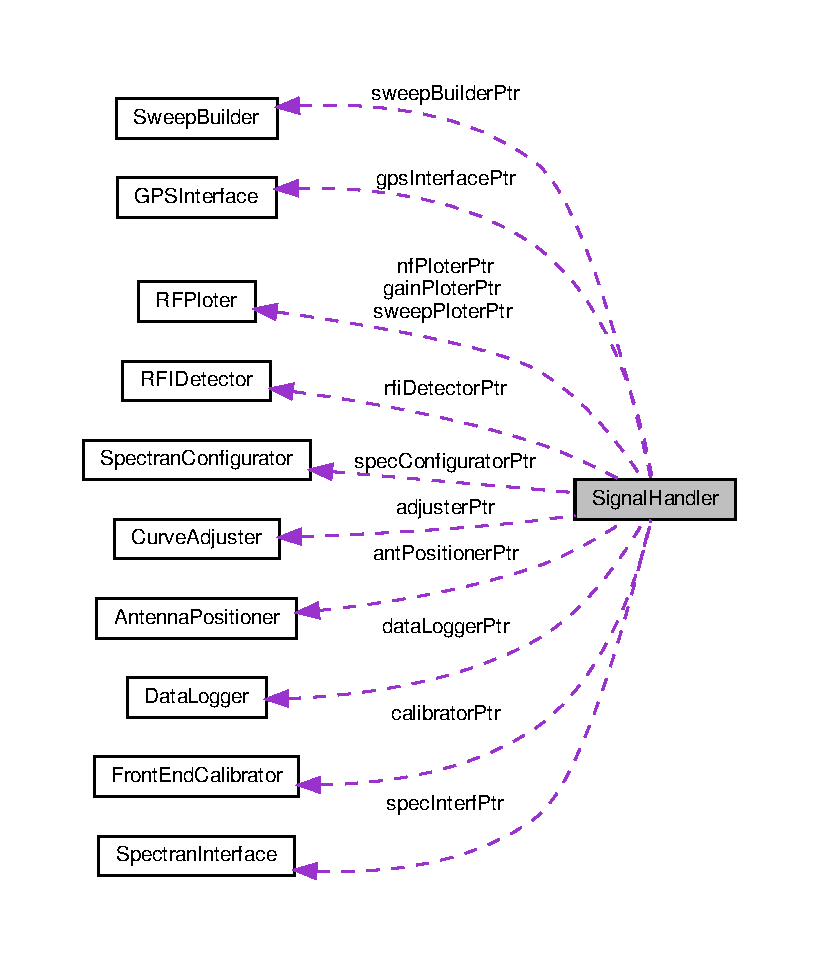
\includegraphics[width=350pt]{classSignalHandler__coll__graph}
\end{center}
\end{figure}
\subsection*{Public Member Functions}
\begin{DoxyCompactItemize}
\item 
\mbox{\Hypertarget{classSignalHandler_aac189962a11b36ed582bd837b99e503b}\label{classSignalHandler_aac189962a11b36ed582bd837b99e503b}} 
void \hyperlink{classSignalHandler_aac189962a11b36ed582bd837b99e503b}{Setup\+Signal\+Handler} (\hyperlink{classSpectranInterface}{Spectran\+Interface} $\ast$spec\+Interf\+Pt, \hyperlink{classSpectranConfigurator}{Spectran\+Configurator} $\ast$spec\+Configurator\+Pt, \hyperlink{classSweepBuilder}{Sweep\+Builder} $\ast$sweep\+Builder\+Pt, \hyperlink{classCurveAdjuster}{Curve\+Adjuster} $\ast$adjuster\+Pt, \hyperlink{classFrontEndCalibrator}{Front\+End\+Calibrator} $\ast$calibrator\+Pt, \hyperlink{classRFIDetector}{R\+F\+I\+Detector} $\ast$rfi\+Detector\+Pt=nullptr, \hyperlink{classDataLogger}{Data\+Logger} $\ast$data\+Logger\+Pt=nullptr, \hyperlink{classGPSInterface}{G\+P\+S\+Interface} $\ast$gps\+Interface\+Pt=nullptr, \hyperlink{classAntennaPositioner}{Antenna\+Positioner} $\ast$ant\+Positioner\+Pt=nullptr, \hyperlink{classRFPloter}{R\+F\+Ploter} $\ast$sweep\+Ploter\+Pt=nullptr, \hyperlink{classRFPloter}{R\+F\+Ploter} $\ast$gain\+Ploter\+Pt=nullptr, \hyperlink{classRFPloter}{R\+F\+Ploter} $\ast$nf\+Ploter\+Pt=nullptr)
\begin{DoxyCompactList}\small\item\em This method is intended to set the pointers to the high-\/level objects and to set handler functions. \end{DoxyCompactList}\end{DoxyCompactItemize}
\subsection*{Static Public Member Functions}
\begin{DoxyCompactItemize}
\item 
static void \hyperlink{classSignalHandler_af32b7213b43fd13fa12587a0c0d9b565}{Exit\+Signal\+Handler} (int signum)
\begin{DoxyCompactList}\small\item\em This function is executed when a S\+I\+G\+I\+NT or a S\+I\+G\+T\+E\+RM signal arrives. \end{DoxyCompactList}\end{DoxyCompactItemize}
\subsection*{Static Public Attributes}
\begin{DoxyCompactItemize}
\item 
static \hyperlink{classSpectranInterface}{Spectran\+Interface} $\ast$ \hyperlink{classSignalHandler_a855d0b79fcbacf50e4a1d12bd5d1bf53}{spec\+Interf\+Ptr}
\begin{DoxyCompactList}\small\item\em A pointer to the {\itshape \hyperlink{classSpectranInterface}{Spectran\+Interface}} object. \end{DoxyCompactList}\item 
static \hyperlink{classSpectranConfigurator}{Spectran\+Configurator} $\ast$ \hyperlink{classSignalHandler_a0b9c75b3e3c928c01cc5e44d42e5ac38}{spec\+Configurator\+Ptr}
\begin{DoxyCompactList}\small\item\em A pointer to the {\itshape \hyperlink{classSpectranConfigurator}{Spectran\+Configurator}} object. \end{DoxyCompactList}\item 
static \hyperlink{classSweepBuilder}{Sweep\+Builder} $\ast$ \hyperlink{classSignalHandler_a23ec28699521fb435a5eb90f2c36bccb}{sweep\+Builder\+Ptr}
\begin{DoxyCompactList}\small\item\em A pointer to the {\itshape \hyperlink{classSweepBuilder}{Sweep\+Builder}} object. \end{DoxyCompactList}\item 
static \hyperlink{classCurveAdjuster}{Curve\+Adjuster} $\ast$ \hyperlink{classSignalHandler_ab3328bb82a0e67153d8ff39bf04c7196}{adjuster\+Ptr}
\begin{DoxyCompactList}\small\item\em A pointer to the {\itshape \hyperlink{classCurveAdjuster}{Curve\+Adjuster}} object. \end{DoxyCompactList}\item 
static \hyperlink{classFrontEndCalibrator}{Front\+End\+Calibrator} $\ast$ \hyperlink{classSignalHandler_ae5bbe309adfefeb3b7e9ebf31d32b763}{calibrator\+Ptr}
\begin{DoxyCompactList}\small\item\em A pointer to the {\itshape \hyperlink{classFrontEndCalibrator}{Front\+End\+Calibrator}} object. \end{DoxyCompactList}\item 
static \hyperlink{classRFIDetector}{R\+F\+I\+Detector} $\ast$ \hyperlink{classSignalHandler_a9ce3533694e1e412496dc5a9b339ccc3}{rfi\+Detector\+Ptr}
\begin{DoxyCompactList}\small\item\em A pointer to the {\itshape \hyperlink{classRFIDetector}{R\+F\+I\+Detector}} object. \end{DoxyCompactList}\item 
static \hyperlink{classDataLogger}{Data\+Logger} $\ast$ \hyperlink{classSignalHandler_a114e600bdc2ad95efbc2991c97f3732c}{data\+Logger\+Ptr}
\begin{DoxyCompactList}\small\item\em A pointer to the {\itshape \hyperlink{classDataLogger}{Data\+Logger}} object. \end{DoxyCompactList}\item 
static \hyperlink{classGPSInterface}{G\+P\+S\+Interface} $\ast$ \hyperlink{classSignalHandler_ac6bc3decceefdff9d3e5c15e4125fe08}{gps\+Interface\+Ptr}
\begin{DoxyCompactList}\small\item\em A pointer to the {\itshape \hyperlink{classGPSInterface}{G\+P\+S\+Interface}} object. \end{DoxyCompactList}\item 
static \hyperlink{classAntennaPositioner}{Antenna\+Positioner} $\ast$ \hyperlink{classSignalHandler_a04f82481d0f5795308e6e2cef7bb0f88}{ant\+Positioner\+Ptr}
\begin{DoxyCompactList}\small\item\em A pointer to the {\itshape \hyperlink{classAntennaPositioner}{Antenna\+Positioner}} object. \end{DoxyCompactList}\item 
static \hyperlink{classRFPloter}{R\+F\+Ploter} $\ast$ \hyperlink{classSignalHandler_a15d34535b8684c5988ff1af1bf6062f6}{sweep\+Ploter\+Ptr}
\begin{DoxyCompactList}\small\item\em A pointer to the {\itshape R\+F\+Plotter} object which is responsible for the plotting of the last captured sweep. \end{DoxyCompactList}\item 
static \hyperlink{classRFPloter}{R\+F\+Ploter} $\ast$ \hyperlink{classSignalHandler_a1c6637986751faafe7cb5ffd58400f77}{gain\+Ploter\+Ptr}
\begin{DoxyCompactList}\small\item\em A pointer to the {\itshape R\+F\+Plotter} object which is responsible for the plotting of the last estimated gain curve. \end{DoxyCompactList}\item 
static \hyperlink{classRFPloter}{R\+F\+Ploter} $\ast$ \hyperlink{classSignalHandler_ada606b8ef692809838f1e5464871742c}{nf\+Ploter\+Ptr}
\begin{DoxyCompactList}\small\item\em A pointer to the {\itshape R\+F\+Plotter} object which is responsible for the plotting of the last estimated noise figure curve. \end{DoxyCompactList}\end{DoxyCompactItemize}


\subsection{Detailed Description}
The class {\itshape \hyperlink{classSignalHandler}{Signal\+Handler}} is intended to handle the interprocess signals (I\+PC) which terminates the software. 

The signals which are handled by this class are S\+I\+G\+I\+NT and S\+I\+G\+T\+E\+RM. When one these signals arrived, the destructors of all the high-\/level objects are called, to ensure a clean closing of the software and an adequate turning off the RF front end. 

\subsection{Member Function Documentation}
\mbox{\Hypertarget{classSignalHandler_af32b7213b43fd13fa12587a0c0d9b565}\label{classSignalHandler_af32b7213b43fd13fa12587a0c0d9b565}} 
\index{Signal\+Handler@{Signal\+Handler}!Exit\+Signal\+Handler@{Exit\+Signal\+Handler}}
\index{Exit\+Signal\+Handler@{Exit\+Signal\+Handler}!Signal\+Handler@{Signal\+Handler}}
\subsubsection{\texorpdfstring{Exit\+Signal\+Handler()}{ExitSignalHandler()}}
{\footnotesize\ttfamily static void Signal\+Handler\+::\+Exit\+Signal\+Handler (\begin{DoxyParamCaption}\item[{int}]{signum }\end{DoxyParamCaption})\hspace{0.3cm}{\ttfamily [inline]}, {\ttfamily [static]}}



This function is executed when a S\+I\+G\+I\+NT or a S\+I\+G\+T\+E\+RM signal arrives. 

The function calls the destructor of almost all the high-\/level objects (defined in the main function) to ensure a clean closing of the software and an adequate turning off the RF front end. 
\begin{DoxyParams}[1]{Parameters}
\mbox{\tt in}  & {\em signum} & This parameters must always be present and it states the number of the arrived signal. \\
\hline
\end{DoxyParams}


\subsection{Member Data Documentation}
\mbox{\Hypertarget{classSignalHandler_ab3328bb82a0e67153d8ff39bf04c7196}\label{classSignalHandler_ab3328bb82a0e67153d8ff39bf04c7196}} 
\index{Signal\+Handler@{Signal\+Handler}!adjuster\+Ptr@{adjuster\+Ptr}}
\index{adjuster\+Ptr@{adjuster\+Ptr}!Signal\+Handler@{Signal\+Handler}}
\subsubsection{\texorpdfstring{adjuster\+Ptr}{adjusterPtr}}
{\footnotesize\ttfamily \hyperlink{classCurveAdjuster}{Curve\+Adjuster} $\ast$ Signal\+Handler\+::adjuster\+Ptr\hspace{0.3cm}{\ttfamily [static]}}



A pointer to the {\itshape \hyperlink{classCurveAdjuster}{Curve\+Adjuster}} object. 

The instantiation of the pointer to the {\itshape Curve\+Ajuster} object. \mbox{\Hypertarget{classSignalHandler_a04f82481d0f5795308e6e2cef7bb0f88}\label{classSignalHandler_a04f82481d0f5795308e6e2cef7bb0f88}} 
\index{Signal\+Handler@{Signal\+Handler}!ant\+Positioner\+Ptr@{ant\+Positioner\+Ptr}}
\index{ant\+Positioner\+Ptr@{ant\+Positioner\+Ptr}!Signal\+Handler@{Signal\+Handler}}
\subsubsection{\texorpdfstring{ant\+Positioner\+Ptr}{antPositionerPtr}}
{\footnotesize\ttfamily \hyperlink{classAntennaPositioner}{Antenna\+Positioner} $\ast$ Signal\+Handler\+::ant\+Positioner\+Ptr\hspace{0.3cm}{\ttfamily [static]}}



A pointer to the {\itshape \hyperlink{classAntennaPositioner}{Antenna\+Positioner}} object. 

The instantiation of the pointer to the {\itshape \hyperlink{classAntennaPositioner}{Antenna\+Positioner}} object. \mbox{\Hypertarget{classSignalHandler_ae5bbe309adfefeb3b7e9ebf31d32b763}\label{classSignalHandler_ae5bbe309adfefeb3b7e9ebf31d32b763}} 
\index{Signal\+Handler@{Signal\+Handler}!calibrator\+Ptr@{calibrator\+Ptr}}
\index{calibrator\+Ptr@{calibrator\+Ptr}!Signal\+Handler@{Signal\+Handler}}
\subsubsection{\texorpdfstring{calibrator\+Ptr}{calibratorPtr}}
{\footnotesize\ttfamily \hyperlink{classFrontEndCalibrator}{Front\+End\+Calibrator} $\ast$ Signal\+Handler\+::calibrator\+Ptr\hspace{0.3cm}{\ttfamily [static]}}



A pointer to the {\itshape \hyperlink{classFrontEndCalibrator}{Front\+End\+Calibrator}} object. 

The instantiation of the pointer to the {\itshape \hyperlink{classFrontEndCalibrator}{Front\+End\+Calibrator}} object. \mbox{\Hypertarget{classSignalHandler_a114e600bdc2ad95efbc2991c97f3732c}\label{classSignalHandler_a114e600bdc2ad95efbc2991c97f3732c}} 
\index{Signal\+Handler@{Signal\+Handler}!data\+Logger\+Ptr@{data\+Logger\+Ptr}}
\index{data\+Logger\+Ptr@{data\+Logger\+Ptr}!Signal\+Handler@{Signal\+Handler}}
\subsubsection{\texorpdfstring{data\+Logger\+Ptr}{dataLoggerPtr}}
{\footnotesize\ttfamily \hyperlink{classDataLogger}{Data\+Logger} $\ast$ Signal\+Handler\+::data\+Logger\+Ptr\hspace{0.3cm}{\ttfamily [static]}}



A pointer to the {\itshape \hyperlink{classDataLogger}{Data\+Logger}} object. 

The instantiation of the pointer to the {\itshape \hyperlink{classDataLogger}{Data\+Logger}} object. \mbox{\Hypertarget{classSignalHandler_a1c6637986751faafe7cb5ffd58400f77}\label{classSignalHandler_a1c6637986751faafe7cb5ffd58400f77}} 
\index{Signal\+Handler@{Signal\+Handler}!gain\+Ploter\+Ptr@{gain\+Ploter\+Ptr}}
\index{gain\+Ploter\+Ptr@{gain\+Ploter\+Ptr}!Signal\+Handler@{Signal\+Handler}}
\subsubsection{\texorpdfstring{gain\+Ploter\+Ptr}{gainPloterPtr}}
{\footnotesize\ttfamily \hyperlink{classRFPloter}{R\+F\+Ploter} $\ast$ Signal\+Handler\+::gain\+Ploter\+Ptr\hspace{0.3cm}{\ttfamily [static]}}



A pointer to the {\itshape R\+F\+Plotter} object which is responsible for the plotting of the last estimated gain curve. 

The instantiation of the pointer to the {\itshape R\+F\+Plotter} object which is responsible for the plotting of the last estimated gain curve. \mbox{\Hypertarget{classSignalHandler_ac6bc3decceefdff9d3e5c15e4125fe08}\label{classSignalHandler_ac6bc3decceefdff9d3e5c15e4125fe08}} 
\index{Signal\+Handler@{Signal\+Handler}!gps\+Interface\+Ptr@{gps\+Interface\+Ptr}}
\index{gps\+Interface\+Ptr@{gps\+Interface\+Ptr}!Signal\+Handler@{Signal\+Handler}}
\subsubsection{\texorpdfstring{gps\+Interface\+Ptr}{gpsInterfacePtr}}
{\footnotesize\ttfamily \hyperlink{classGPSInterface}{G\+P\+S\+Interface} $\ast$ Signal\+Handler\+::gps\+Interface\+Ptr\hspace{0.3cm}{\ttfamily [static]}}



A pointer to the {\itshape \hyperlink{classGPSInterface}{G\+P\+S\+Interface}} object. 

The instantiation of the pointer to the {\itshape \hyperlink{classGPSInterface}{G\+P\+S\+Interface}} object. \mbox{\Hypertarget{classSignalHandler_ada606b8ef692809838f1e5464871742c}\label{classSignalHandler_ada606b8ef692809838f1e5464871742c}} 
\index{Signal\+Handler@{Signal\+Handler}!nf\+Ploter\+Ptr@{nf\+Ploter\+Ptr}}
\index{nf\+Ploter\+Ptr@{nf\+Ploter\+Ptr}!Signal\+Handler@{Signal\+Handler}}
\subsubsection{\texorpdfstring{nf\+Ploter\+Ptr}{nfPloterPtr}}
{\footnotesize\ttfamily \hyperlink{classRFPloter}{R\+F\+Ploter} $\ast$ Signal\+Handler\+::nf\+Ploter\+Ptr\hspace{0.3cm}{\ttfamily [static]}}



A pointer to the {\itshape R\+F\+Plotter} object which is responsible for the plotting of the last estimated noise figure curve. 

The instantiation of the pointer to the {\itshape R\+F\+Plotter} object which is responsible for the plotting of the last estimated noise figure curve. \mbox{\Hypertarget{classSignalHandler_a9ce3533694e1e412496dc5a9b339ccc3}\label{classSignalHandler_a9ce3533694e1e412496dc5a9b339ccc3}} 
\index{Signal\+Handler@{Signal\+Handler}!rfi\+Detector\+Ptr@{rfi\+Detector\+Ptr}}
\index{rfi\+Detector\+Ptr@{rfi\+Detector\+Ptr}!Signal\+Handler@{Signal\+Handler}}
\subsubsection{\texorpdfstring{rfi\+Detector\+Ptr}{rfiDetectorPtr}}
{\footnotesize\ttfamily \hyperlink{classRFIDetector}{R\+F\+I\+Detector} $\ast$ Signal\+Handler\+::rfi\+Detector\+Ptr\hspace{0.3cm}{\ttfamily [static]}}



A pointer to the {\itshape \hyperlink{classRFIDetector}{R\+F\+I\+Detector}} object. 

The instantiation of the pointer to the {\itshape \hyperlink{classRFIDetector}{R\+F\+I\+Detector}} object. \mbox{\Hypertarget{classSignalHandler_a0b9c75b3e3c928c01cc5e44d42e5ac38}\label{classSignalHandler_a0b9c75b3e3c928c01cc5e44d42e5ac38}} 
\index{Signal\+Handler@{Signal\+Handler}!spec\+Configurator\+Ptr@{spec\+Configurator\+Ptr}}
\index{spec\+Configurator\+Ptr@{spec\+Configurator\+Ptr}!Signal\+Handler@{Signal\+Handler}}
\subsubsection{\texorpdfstring{spec\+Configurator\+Ptr}{specConfiguratorPtr}}
{\footnotesize\ttfamily \hyperlink{classSpectranConfigurator}{Spectran\+Configurator} $\ast$ Signal\+Handler\+::spec\+Configurator\+Ptr\hspace{0.3cm}{\ttfamily [static]}}



A pointer to the {\itshape \hyperlink{classSpectranConfigurator}{Spectran\+Configurator}} object. 

The instantiation of the pointer to the {\itshape \hyperlink{classSpectranConfigurator}{Spectran\+Configurator}} object. \mbox{\Hypertarget{classSignalHandler_a855d0b79fcbacf50e4a1d12bd5d1bf53}\label{classSignalHandler_a855d0b79fcbacf50e4a1d12bd5d1bf53}} 
\index{Signal\+Handler@{Signal\+Handler}!spec\+Interf\+Ptr@{spec\+Interf\+Ptr}}
\index{spec\+Interf\+Ptr@{spec\+Interf\+Ptr}!Signal\+Handler@{Signal\+Handler}}
\subsubsection{\texorpdfstring{spec\+Interf\+Ptr}{specInterfPtr}}
{\footnotesize\ttfamily \hyperlink{classSpectranInterface}{Spectran\+Interface} $\ast$ Signal\+Handler\+::spec\+Interf\+Ptr\hspace{0.3cm}{\ttfamily [static]}}



A pointer to the {\itshape \hyperlink{classSpectranInterface}{Spectran\+Interface}} object. 

The instantiation of the pointer to the {\itshape \hyperlink{classSpectranInterface}{Spectran\+Interface}} object. \mbox{\Hypertarget{classSignalHandler_a23ec28699521fb435a5eb90f2c36bccb}\label{classSignalHandler_a23ec28699521fb435a5eb90f2c36bccb}} 
\index{Signal\+Handler@{Signal\+Handler}!sweep\+Builder\+Ptr@{sweep\+Builder\+Ptr}}
\index{sweep\+Builder\+Ptr@{sweep\+Builder\+Ptr}!Signal\+Handler@{Signal\+Handler}}
\subsubsection{\texorpdfstring{sweep\+Builder\+Ptr}{sweepBuilderPtr}}
{\footnotesize\ttfamily \hyperlink{classSweepBuilder}{Sweep\+Builder} $\ast$ Signal\+Handler\+::sweep\+Builder\+Ptr\hspace{0.3cm}{\ttfamily [static]}}



A pointer to the {\itshape \hyperlink{classSweepBuilder}{Sweep\+Builder}} object. 

The instantiation of the pointer to the {\itshape \hyperlink{classSweepBuilder}{Sweep\+Builder}} object. \mbox{\Hypertarget{classSignalHandler_a15d34535b8684c5988ff1af1bf6062f6}\label{classSignalHandler_a15d34535b8684c5988ff1af1bf6062f6}} 
\index{Signal\+Handler@{Signal\+Handler}!sweep\+Ploter\+Ptr@{sweep\+Ploter\+Ptr}}
\index{sweep\+Ploter\+Ptr@{sweep\+Ploter\+Ptr}!Signal\+Handler@{Signal\+Handler}}
\subsubsection{\texorpdfstring{sweep\+Ploter\+Ptr}{sweepPloterPtr}}
{\footnotesize\ttfamily \hyperlink{classRFPloter}{R\+F\+Ploter} $\ast$ Signal\+Handler\+::sweep\+Ploter\+Ptr\hspace{0.3cm}{\ttfamily [static]}}



A pointer to the {\itshape R\+F\+Plotter} object which is responsible for the plotting of the last captured sweep. 

The instantiation of the pointer to the {\itshape R\+F\+Plotter} object which is responsible for the plotting of the last captured sweep. 

The documentation for this class was generated from the following files\+:\begin{DoxyCompactItemize}
\item 
/home/new-\/mauro/eclipse-\/cdt/workspace/\+R\+F\+I\+M\+S\+\_\+\+C\+A\+R\+T/src/\hyperlink{TopLevel_8h}{Top\+Level.\+h}\item 
/home/new-\/mauro/eclipse-\/cdt/workspace/\+R\+F\+I\+M\+S\+\_\+\+C\+A\+R\+T/src/\hyperlink{main_8cpp}{main.\+cpp}\end{DoxyCompactItemize}

\hypertarget{classSpectranConfigurator}{}\section{Spectran\+Configurator Class Reference}
\label{classSpectranConfigurator}\index{Spectran\+Configurator@{Spectran\+Configurator}}


The class {\itshape \hyperlink{classSpectranConfigurator}{Spectran\+Configurator}} is intended to manage the process of configuring the Aaronia Spectran device.  




{\ttfamily \#include $<$Spectran.\+h$>$}

\subsection*{Classes}
\begin{DoxyCompactItemize}
\item 
struct \hyperlink{structSpectranConfigurator_1_1FixedParameters}{Fixed\+Parameters}
\begin{DoxyCompactList}\small\item\em This structure saves the fixed parameters of the spectrum analyzer, i.\+e. the parameters which do not change through the entire measurement cycle. \end{DoxyCompactList}\end{DoxyCompactItemize}
\subsection*{Public Member Functions}
\begin{DoxyCompactItemize}
\item 
\hyperlink{classSpectranConfigurator_af6a9f524ea5625e6e30be0e843c17c8a}{Spectran\+Configurator} (\hyperlink{classSpectranInterface}{Spectran\+Interface} \&interf)
\begin{DoxyCompactList}\small\item\em The default constructor. \end{DoxyCompactList}\item 
\mbox{\Hypertarget{classSpectranConfigurator_aa697b14d994a5d0fabe2639036f70dc8}\label{classSpectranConfigurator_aa697b14d994a5d0fabe2639036f70dc8}} 
\hyperlink{classSpectranConfigurator_aa697b14d994a5d0fabe2639036f70dc8}{$\sim$\+Spectran\+Configurator} ()
\begin{DoxyCompactList}\small\item\em The destructor which just makes sure the input file stream is closed. \end{DoxyCompactList}\item 
bool \hyperlink{classSpectranConfigurator_ab3dfc0843d10b2e9bad09f599165d6ff}{Load\+Fixed\+Parameters} ()
\begin{DoxyCompactList}\small\item\em This method loads the fixed Spectran\textquotesingle{}s parameters from the corresponding file. \end{DoxyCompactList}\item 
bool \hyperlink{classSpectranConfigurator_a9171d48390718bd6f2d05922ee6596cd}{Load\+Bands\+Parameters} ()
\begin{DoxyCompactList}\small\item\em This method loads the frequency bands parameters from the corresponding file. \end{DoxyCompactList}\item 
void \hyperlink{classSpectranConfigurator_ad2deb73f4c1691cd8bff29b810f8f42b}{Initial\+Configuration} ()
\begin{DoxyCompactList}\small\item\em This method is intended to configure the spectrum analyzer with the fixed parameters at the beginning of a measurement cycle. \end{DoxyCompactList}\item 
\hyperlink{structBandParameters}{Band\+Parameters} \hyperlink{classSpectranConfigurator_a4bea5937bcf7c904c3eb435a2d25e3fb}{Configure\+Next\+Band} ()
\begin{DoxyCompactList}\small\item\em The aim of this method is to configure the spectrum analyzer with parameters of the next frequency band. \end{DoxyCompactList}\item 
void \hyperlink{classSpectranConfigurator_a7402a16a8514a0c1b230164b7f5d9d21}{Set\+Curr\+Band\+Parameters} (const \hyperlink{structBandParameters}{Band\+Parameters} \&curr\+Band\+Param)
\begin{DoxyCompactList}\small\item\em This method allows to change the parameters of the current frequency band, given a {\itshape \hyperlink{structBandParameters}{Band\+Parameters}} structure as parameter. \end{DoxyCompactList}\item 
\mbox{\Hypertarget{classSpectranConfigurator_a4d5f0fc0842d96bdaef2555f63cd5ad6}\label{classSpectranConfigurator_a4d5f0fc0842d96bdaef2555f63cd5ad6}} 
const \hyperlink{structSpectranConfigurator_1_1FixedParameters}{Fixed\+Parameters} \& \hyperlink{classSpectranConfigurator_a4d5f0fc0842d96bdaef2555f63cd5ad6}{Get\+Fixed\+Parameters} () const
\begin{DoxyCompactList}\small\item\em This method returns the fixed parameters. \end{DoxyCompactList}\item 
\mbox{\Hypertarget{classSpectranConfigurator_a8d7445409e7e019d9763228343d04c5f}\label{classSpectranConfigurator_a8d7445409e7e019d9763228343d04c5f}} 
const std\+::vector$<$ \hyperlink{structBandParameters}{Band\+Parameters} $>$ \& \hyperlink{classSpectranConfigurator_a8d7445409e7e019d9763228343d04c5f}{Get\+Bands\+Parameters} () const
\begin{DoxyCompactList}\small\item\em This method returns a vector with the parameters of all frequency bands. \end{DoxyCompactList}\item 
\mbox{\Hypertarget{classSpectranConfigurator_a9349287cdb255852996aa5b07e83bf0d}\label{classSpectranConfigurator_a9349287cdb255852996aa5b07e83bf0d}} 
const std\+::vector$<$ \hyperlink{structBandParameters}{Band\+Parameters} $>$ \& \hyperlink{classSpectranConfigurator_a9349287cdb255852996aa5b07e83bf0d}{Get\+Sub\+Bands\+Parameters} () const
\begin{DoxyCompactList}\small\item\em This method returns a vector with the parameters of all frequency sub-\/bands. \end{DoxyCompactList}\item 
\mbox{\Hypertarget{classSpectranConfigurator_ad9d3fa35d5fbca578a8e503a4eaff97f}\label{classSpectranConfigurator_ad9d3fa35d5fbca578a8e503a4eaff97f}} 
const \hyperlink{structBandParameters}{Band\+Parameters} \& \hyperlink{classSpectranConfigurator_ad9d3fa35d5fbca578a8e503a4eaff97f}{Get\+Curr\+Band\+Parameters} () const
\begin{DoxyCompactList}\small\item\em This method returns the parameters of the current frequency band. \end{DoxyCompactList}\item 
\mbox{\Hypertarget{classSpectranConfigurator_ad76d87b5f229c12dbf378dcf3f9fbf52}\label{classSpectranConfigurator_ad76d87b5f229c12dbf378dcf3f9fbf52}} 
unsigned int \hyperlink{classSpectranConfigurator_ad76d87b5f229c12dbf378dcf3f9fbf52}{Get\+Num\+Of\+Bands} () const
\begin{DoxyCompactList}\small\item\em This method returns the number of frequency sub-\/bands (or bands if they were not split). \end{DoxyCompactList}\item 
\mbox{\Hypertarget{classSpectranConfigurator_a72997f08ddcf4bbcfa4d1bfa632ac002}\label{classSpectranConfigurator_a72997f08ddcf4bbcfa4d1bfa632ac002}} 
unsigned int \hyperlink{classSpectranConfigurator_a72997f08ddcf4bbcfa4d1bfa632ac002}{Get\+Band\+Index} () const
\begin{DoxyCompactList}\small\item\em This method returns the current value of the band index. \end{DoxyCompactList}\item 
\mbox{\Hypertarget{classSpectranConfigurator_afe7186f4e99bf125f2301ce411a8c559}\label{classSpectranConfigurator_afe7186f4e99bf125f2301ce411a8c559}} 
bool \hyperlink{classSpectranConfigurator_afe7186f4e99bf125f2301ce411a8c559}{Is\+Last\+Band} () const
\begin{DoxyCompactList}\small\item\em This method returns a {\ttfamily true} if the current band is the last one and a {\ttfamily false} otherwise. \end{DoxyCompactList}\end{DoxyCompactItemize}


\subsection{Detailed Description}
The class {\itshape \hyperlink{classSpectranConfigurator}{Spectran\+Configurator}} is intended to manage the process of configuring the Aaronia Spectran device. 

To do this task, this component give {\itshape \hyperlink{classCommand}{Command}} objects to the {\itshape \hyperlink{classSpectranInterface}{Spectran\+Interface}} object, which writes them in the spectrum analyzer and then it reads the replies, the Spectran Interface passes them as {\itshape \hyperlink{classReply}{Reply}} objects to the Spectran Configurator, so this one can know if the last configuration was performed successfully or not. 

\subsection{Constructor \& Destructor Documentation}
\mbox{\Hypertarget{classSpectranConfigurator_af6a9f524ea5625e6e30be0e843c17c8a}\label{classSpectranConfigurator_af6a9f524ea5625e6e30be0e843c17c8a}} 
\index{Spectran\+Configurator@{Spectran\+Configurator}!Spectran\+Configurator@{Spectran\+Configurator}}
\index{Spectran\+Configurator@{Spectran\+Configurator}!Spectran\+Configurator@{Spectran\+Configurator}}
\subsubsection{\texorpdfstring{Spectran\+Configurator()}{SpectranConfigurator()}}
{\footnotesize\ttfamily Spectran\+Configurator\+::\+Spectran\+Configurator (\begin{DoxyParamCaption}\item[{\hyperlink{classSpectranInterface}{Spectran\+Interface} \&}]{interf }\end{DoxyParamCaption})}



The default constructor. 

At instantiation of an object, a reference to the {\itshape \hyperlink{classSpectranInterface}{Spectran\+Interface}} object must be given. 
\begin{DoxyParams}[1]{Parameters}
\mbox{\tt in}  & {\em interf} & A reference to the unique {\itshape \hyperlink{classSpectranInterface}{Spectran\+Interface}} object, which is responsible for the communication with the spectrum analyzer. \\
\hline
\end{DoxyParams}


\subsection{Member Function Documentation}
\mbox{\Hypertarget{classSpectranConfigurator_a4bea5937bcf7c904c3eb435a2d25e3fb}\label{classSpectranConfigurator_a4bea5937bcf7c904c3eb435a2d25e3fb}} 
\index{Spectran\+Configurator@{Spectran\+Configurator}!Configure\+Next\+Band@{Configure\+Next\+Band}}
\index{Configure\+Next\+Band@{Configure\+Next\+Band}!Spectran\+Configurator@{Spectran\+Configurator}}
\subsubsection{\texorpdfstring{Configure\+Next\+Band()}{ConfigureNextBand()}}
{\footnotesize\ttfamily \hyperlink{structBandParameters}{Band\+Parameters} Spectran\+Configurator\+::\+Configure\+Next\+Band (\begin{DoxyParamCaption}{ }\end{DoxyParamCaption})}



The aim of this method is to configure the spectrum analyzer with parameters of the next frequency band. 

The first time this method is called, it configures the spectrum analyzer with the first band\textquotesingle{}s parameters. Then, it will increase the band index to move to the parameters of the next band. Again, the streaming of sweep points should be disabled before calling this method.

This method returns the parameters of the current frequency band as a {\itshape \hyperlink{structBandParameters}{Band\+Parameters}} structure. \mbox{\Hypertarget{classSpectranConfigurator_ad2deb73f4c1691cd8bff29b810f8f42b}\label{classSpectranConfigurator_ad2deb73f4c1691cd8bff29b810f8f42b}} 
\index{Spectran\+Configurator@{Spectran\+Configurator}!Initial\+Configuration@{Initial\+Configuration}}
\index{Initial\+Configuration@{Initial\+Configuration}!Spectran\+Configurator@{Spectran\+Configurator}}
\subsubsection{\texorpdfstring{Initial\+Configuration()}{InitialConfiguration()}}
{\footnotesize\ttfamily void Spectran\+Configurator\+::\+Initial\+Configuration (\begin{DoxyParamCaption}{ }\end{DoxyParamCaption})}



This method is intended to configure the spectrum analyzer with the fixed parameters at the beginning of a measurement cycle. 

This method should be used at the beginning of the first measurement cycle and at beginning of rest ones if the file with the fixed parameters has been modified. Obviously, the sending of measurements via U\+SB must be disable before calling this method. \mbox{\Hypertarget{classSpectranConfigurator_a9171d48390718bd6f2d05922ee6596cd}\label{classSpectranConfigurator_a9171d48390718bd6f2d05922ee6596cd}} 
\index{Spectran\+Configurator@{Spectran\+Configurator}!Load\+Bands\+Parameters@{Load\+Bands\+Parameters}}
\index{Load\+Bands\+Parameters@{Load\+Bands\+Parameters}!Spectran\+Configurator@{Spectran\+Configurator}}
\subsubsection{\texorpdfstring{Load\+Bands\+Parameters()}{LoadBandsParameters()}}
{\footnotesize\ttfamily bool Spectran\+Configurator\+::\+Load\+Bands\+Parameters (\begin{DoxyParamCaption}{ }\end{DoxyParamCaption})}



This method loads the frequency bands parameters from the corresponding file. 

The method loads the parameters of one band, stores them in a structure {\itshape Bands\+Parameters} and then it splits the band in several sub-\/bands, if its span is bigger than 200 M\+Hz. Then it moves to next frequency band until the end-\/of-\/file (E\+OF) is reached.

The method returns a {\ttfamily true} if the parameters were loaded from the file, either because it is the first time they are read or because the corresponding file was modified. If the parameters had been loaded before and it was found that the file was not modified from the last loading, the parameters are not read from the file and the method returns a {\ttfamily false}. \mbox{\Hypertarget{classSpectranConfigurator_ab3dfc0843d10b2e9bad09f599165d6ff}\label{classSpectranConfigurator_ab3dfc0843d10b2e9bad09f599165d6ff}} 
\index{Spectran\+Configurator@{Spectran\+Configurator}!Load\+Fixed\+Parameters@{Load\+Fixed\+Parameters}}
\index{Load\+Fixed\+Parameters@{Load\+Fixed\+Parameters}!Spectran\+Configurator@{Spectran\+Configurator}}
\subsubsection{\texorpdfstring{Load\+Fixed\+Parameters()}{LoadFixedParameters()}}
{\footnotesize\ttfamily bool Spectran\+Configurator\+::\+Load\+Fixed\+Parameters (\begin{DoxyParamCaption}{ }\end{DoxyParamCaption})}



This method loads the fixed Spectran\textquotesingle{}s parameters from the corresponding file. 

The method returns a boolean value to indicate if the fixed parameters have been updated so the initial configuration should be repeated. The method returns a {\ttfamily true} if the parameters were loaded from the file, either because it is the first time they are read or because the corresponding file was modified. If the parameters had been loaded before and it was found that the file was not modified from the last loading, the parameters are not read from the file and the method returns a {\ttfamily false}. \mbox{\Hypertarget{classSpectranConfigurator_a7402a16a8514a0c1b230164b7f5d9d21}\label{classSpectranConfigurator_a7402a16a8514a0c1b230164b7f5d9d21}} 
\index{Spectran\+Configurator@{Spectran\+Configurator}!Set\+Curr\+Band\+Parameters@{Set\+Curr\+Band\+Parameters}}
\index{Set\+Curr\+Band\+Parameters@{Set\+Curr\+Band\+Parameters}!Spectran\+Configurator@{Spectran\+Configurator}}
\subsubsection{\texorpdfstring{Set\+Curr\+Band\+Parameters()}{SetCurrBandParameters()}}
{\footnotesize\ttfamily void Spectran\+Configurator\+::\+Set\+Curr\+Band\+Parameters (\begin{DoxyParamCaption}\item[{const \hyperlink{structBandParameters}{Band\+Parameters} \&}]{curr\+Band\+Param }\end{DoxyParamCaption})\hspace{0.3cm}{\ttfamily [inline]}}



This method allows to change the parameters of the current frequency band, given a {\itshape \hyperlink{structBandParameters}{Band\+Parameters}} structure as parameter. 


\begin{DoxyParams}[1]{Parameters}
\mbox{\tt in}  & {\em curr\+Band\+Param} & A {\itshape \hyperlink{structBandParameters}{Band\+Parameters}} structure with the parameters which it is desired the current frequency band to have. \\
\hline
\end{DoxyParams}


The documentation for this class was generated from the following files\+:\begin{DoxyCompactItemize}
\item 
/home/new-\/mauro/eclipse-\/cdt/workspace/\+R\+F\+I\+M\+S\+\_\+\+C\+A\+R\+T/src/\hyperlink{Spectran_8h}{Spectran.\+h}\item 
/home/new-\/mauro/eclipse-\/cdt/workspace/\+R\+F\+I\+M\+S\+\_\+\+C\+A\+R\+T/src/\hyperlink{SpectranConfigurator_8cpp}{Spectran\+Configurator.\+cpp}\end{DoxyCompactItemize}

\hypertarget{classSpectranInterface}{}\section{Spectran\+Interface Class Reference}
\label{classSpectranInterface}\index{Spectran\+Interface@{Spectran\+Interface}}


The aim of this class is to manage the communication with the Aaronia Spectran device.  




{\ttfamily \#include $<$Spectran.\+h$>$}

\subsection*{Public Member Functions}
\begin{DoxyCompactItemize}
\item 
\hyperlink{classSpectranInterface_a9ace3807dcbbf01313890871d6a60f51}{Spectran\+Interface} ()
\begin{DoxyCompactList}\small\item\em The default class constructor. \end{DoxyCompactList}\item 
\hyperlink{classSpectranInterface_a52592fb5fe9d7734d869540826b47325}{$\sim$\+Spectran\+Interface} ()
\begin{DoxyCompactList}\small\item\em The class destructor. \end{DoxyCompactList}\item 
void \hyperlink{classSpectranInterface_a29d4a40c802f909b19014a5bfdac7db5}{Initialize} ()
\begin{DoxyCompactList}\small\item\em This method logs in with the spectrum analyzer, once the communication has been opened and its parameters has been set up. \end{DoxyCompactList}\item 
\mbox{\Hypertarget{classSpectranInterface_a31b64b69e1d99723fea1fd9c112dcfda}\label{classSpectranInterface_a31b64b69e1d99723fea1fd9c112dcfda}} 
unsigned int \hyperlink{classSpectranInterface_a31b64b69e1d99723fea1fd9c112dcfda}{Available} ()
\begin{DoxyCompactList}\small\item\em This method returns the number of available bytes in the input buffer. \end{DoxyCompactList}\item 
void \hyperlink{classSpectranInterface_a512218c4f1589c32b4fd9a0f7ad5e8cc}{Reset\+Sweep} ()
\begin{DoxyCompactList}\small\item\em This method is intended to restore the streaming of sweep points to the first point which corresponds to the initial frequency (Fstart). \end{DoxyCompactList}\item 
void \hyperlink{classSpectranInterface_ac812a1bcaede6504f62cc544c30fffea}{Enable\+Sweep} ()
\begin{DoxyCompactList}\small\item\em This method allows to enable the streaming of sweep points. \end{DoxyCompactList}\item 
void \hyperlink{classSpectranInterface_a68b1b1a6af802369cb146c69161d031d}{Disable\+Sweep} ()
\begin{DoxyCompactList}\small\item\em This method allows to disable the streaming of sweep points. \end{DoxyCompactList}\item 
\mbox{\Hypertarget{classSpectranInterface_a67de35ac5416ab4e7880ee03fcd2884e}\label{classSpectranInterface_a67de35ac5416ab4e7880ee03fcd2884e}} 
void \hyperlink{classSpectranInterface_a67de35ac5416ab4e7880ee03fcd2884e}{Purge} ()
\begin{DoxyCompactList}\small\item\em This method purges the input buffer. \end{DoxyCompactList}\item 
void \hyperlink{classSpectranInterface_a59eff163ecf77f55bba22f49ef79d909}{Soft\+Reset} ()
\begin{DoxyCompactList}\small\item\em The soft reset is performed using the function {\ttfamily F\+T\+\_\+\+Reset\+Device()} of the driver D2\+XX. \end{DoxyCompactList}\item 
void \hyperlink{classSpectranInterface_a44ee786fb582c5db42253ec0c96f3b8e}{Hard\+Reset} ()
\begin{DoxyCompactList}\small\item\em The hard reset implies that the spectrum analyzer is turned off and then it is turned on again. \end{DoxyCompactList}\item 
void \hyperlink{classSpectranInterface_a8884f03d3075589a2850c83c9fd57e72}{Log\+Out} ()
\begin{DoxyCompactList}\small\item\em This method finishes the communication session with the spectrum analyzer. \end{DoxyCompactList}\item 
\mbox{\Hypertarget{classSpectranInterface_a7c7d78879a60f850b866386ad6101e20}\label{classSpectranInterface_a7c7d78879a60f850b866386ad6101e20}} 
D\+W\+O\+RD \hyperlink{classSpectranInterface_a7c7d78879a60f850b866386ad6101e20}{Get\+V\+ID} () const
\begin{DoxyCompactList}\small\item\em This method returns the Vendor ID of the spectrum analyzer. \end{DoxyCompactList}\item 
\mbox{\Hypertarget{classSpectranInterface_a70e03dced69c7c7c60951692894d26ce}\label{classSpectranInterface_a70e03dced69c7c7c60951692894d26ce}} 
D\+W\+O\+RD \hyperlink{classSpectranInterface_a70e03dced69c7c7c60951692894d26ce}{Get\+P\+ID} () const
\begin{DoxyCompactList}\small\item\em This method returns the Product ID of the spectrum analyzer. \end{DoxyCompactList}\item 
\mbox{\Hypertarget{classSpectranInterface_a37854d2e596c8338c0015d8ec9120cae}\label{classSpectranInterface_a37854d2e596c8338c0015d8ec9120cae}} 
std\+::string \hyperlink{classSpectranInterface_a37854d2e596c8338c0015d8ec9120cae}{Get\+Dev\+Description} () const
\begin{DoxyCompactList}\small\item\em This method returns the device description (a string) of the spectrum analyzer. \end{DoxyCompactList}\item 
\mbox{\Hypertarget{classSpectranInterface_a7e80df1d7f5709f2976847ee1c91a85d}\label{classSpectranInterface_a7e80df1d7f5709f2976847ee1c91a85d}} 
bool \hyperlink{classSpectranInterface_a7e80df1d7f5709f2976847ee1c91a85d}{Is\+Logged} () const
\begin{DoxyCompactList}\small\item\em This method returns a true value if the communication has been opened and a login has been performed, and a false value otherwise. \end{DoxyCompactList}\item 
\mbox{\Hypertarget{classSpectranInterface_ad921e08380e246d03d01b4ad080cec99}\label{classSpectranInterface_ad921e08380e246d03d01b4ad080cec99}} 
bool \hyperlink{classSpectranInterface_ad921e08380e246d03d01b4ad080cec99}{Is\+Sweep\+Enabled} () const
\begin{DoxyCompactList}\small\item\em This method returns a true value if the streaming of sweep points has been enabled and a false otherwise. \end{DoxyCompactList}\item 
void \hyperlink{classSpectranInterface_a6064f5888f86d0913b8c2af429bdf278}{Sound\+New\+Sweep} ()
\begin{DoxyCompactList}\small\item\em This method allows to perform the a sound to state the capturing of a sweep has finished. \end{DoxyCompactList}\item 
void \hyperlink{classSpectranInterface_a3046fce691a5ed248e3fd647b0b043e8}{Write} (const \hyperlink{classCommand}{Command} \&command)
\begin{DoxyCompactList}\small\item\em This method is intended to perform all the writing operations. \end{DoxyCompactList}\item 
void \hyperlink{classSpectranInterface_a63c61d4d26c5aa335c6a20f469f3ec00}{Read} (\hyperlink{classReply}{Reply} \&reply)
\begin{DoxyCompactList}\small\item\em This method is intended to perform all the reading operations. \end{DoxyCompactList}\end{DoxyCompactItemize}


\subsection{Detailed Description}
The aim of this class is to manage the communication with the Aaronia Spectran device. 

This class establishes the communication with the Aaronia Spectran device (V\+ID=0403, P\+ID=E8\+D8) and allows to write commands to the device and read its replies. Also, it allows to know the available bytes in the input buffer, purge that buffer and reset the communication with the device. 

\subsection{Constructor \& Destructor Documentation}
\mbox{\Hypertarget{classSpectranInterface_a9ace3807dcbbf01313890871d6a60f51}\label{classSpectranInterface_a9ace3807dcbbf01313890871d6a60f51}} 
\index{Spectran\+Interface@{Spectran\+Interface}!Spectran\+Interface@{Spectran\+Interface}}
\index{Spectran\+Interface@{Spectran\+Interface}!Spectran\+Interface@{Spectran\+Interface}}
\subsubsection{\texorpdfstring{Spectran\+Interface()}{SpectranInterface()}}
{\footnotesize\ttfamily Spectran\+Interface\+::\+Spectran\+Interface (\begin{DoxyParamCaption}{ }\end{DoxyParamCaption})}



The default class constructor. 

This constructor initializes the internal flags, flag\+Log\+In and flag\+Sweeps\+Enabled, as false, includes the V\+ID and P\+ID of the spectrum analyzer in the list of possible values and, finally, it calls the method {\ttfamily Open\+And\+Set\+Up()}. \mbox{\Hypertarget{classSpectranInterface_a52592fb5fe9d7734d869540826b47325}\label{classSpectranInterface_a52592fb5fe9d7734d869540826b47325}} 
\index{Spectran\+Interface@{Spectran\+Interface}!````~Spectran\+Interface@{$\sim$\+Spectran\+Interface}}
\index{````~Spectran\+Interface@{$\sim$\+Spectran\+Interface}!Spectran\+Interface@{Spectran\+Interface}}
\subsubsection{\texorpdfstring{$\sim$\+Spectran\+Interface()}{~SpectranInterface()}}
{\footnotesize\ttfamily Spectran\+Interface\+::$\sim$\+Spectran\+Interface (\begin{DoxyParamCaption}{ }\end{DoxyParamCaption})}



The class destructor. 

The destructor carry out the logging out and the communication closing. In each operation, this method produces messages in the {\ttfamily stdout} if there were errors, but it never produces exceptions. 

\subsection{Member Function Documentation}
\mbox{\Hypertarget{classSpectranInterface_a68b1b1a6af802369cb146c69161d031d}\label{classSpectranInterface_a68b1b1a6af802369cb146c69161d031d}} 
\index{Spectran\+Interface@{Spectran\+Interface}!Disable\+Sweep@{Disable\+Sweep}}
\index{Disable\+Sweep@{Disable\+Sweep}!Spectran\+Interface@{Spectran\+Interface}}
\subsubsection{\texorpdfstring{Disable\+Sweep()}{DisableSweep()}}
{\footnotesize\ttfamily void Spectran\+Interface\+::\+Disable\+Sweep (\begin{DoxyParamCaption}{ }\end{DoxyParamCaption})}



This method allows to disable the streaming of sweep points. 

To ensure the streaming is disabled at least two commands (U\+S\+M\+E\+AS, 0) must be sent because the first one will receive a wrong reply as there is a delay until the spectrum analyzer stops sending sweep points (A\+M\+P\+F\+R\+E\+Q\+D\+AT), so the reply to first command will be mixed with the sweep points and the software will read it with errors. Because of that, this method is implemented with a loop where it is tried to disable the streaming times, up to 4 times. After the streaming is disabled successfully, the input buffer is purged. \mbox{\Hypertarget{classSpectranInterface_ac812a1bcaede6504f62cc544c30fffea}\label{classSpectranInterface_ac812a1bcaede6504f62cc544c30fffea}} 
\index{Spectran\+Interface@{Spectran\+Interface}!Enable\+Sweep@{Enable\+Sweep}}
\index{Enable\+Sweep@{Enable\+Sweep}!Spectran\+Interface@{Spectran\+Interface}}
\subsubsection{\texorpdfstring{Enable\+Sweep()}{EnableSweep()}}
{\footnotesize\ttfamily void Spectran\+Interface\+::\+Enable\+Sweep (\begin{DoxyParamCaption}{ }\end{DoxyParamCaption})}



This method allows to enable the streaming of sweep points. 

Take into account that once the streaming the sweep points is enabled, the spectrum analyzer will send these points autonomously, i.\+e. the communication will not follow anymore the master-\/slave paradigm where the slave only sends data to the master when this sends a request. So the software must be prepared to receive and process the data stream. \mbox{\Hypertarget{classSpectranInterface_a44ee786fb582c5db42253ec0c96f3b8e}\label{classSpectranInterface_a44ee786fb582c5db42253ec0c96f3b8e}} 
\index{Spectran\+Interface@{Spectran\+Interface}!Hard\+Reset@{Hard\+Reset}}
\index{Hard\+Reset@{Hard\+Reset}!Spectran\+Interface@{Spectran\+Interface}}
\subsubsection{\texorpdfstring{Hard\+Reset()}{HardReset()}}
{\footnotesize\ttfamily void Spectran\+Interface\+::\+Hard\+Reset (\begin{DoxyParamCaption}{ }\end{DoxyParamCaption})}



The hard reset implies that the spectrum analyzer is turned off and then it is turned on again. 

To start, a logout is performed, then the communication is closed, the entire RF front end is turned off sequentially, then it is waited 10 seconds, the entire front end is turned on again sequentially, and finally the communication is opened again. After the calling of this method, a login must be performed calling the method \hyperlink{classSpectranInterface_a29d4a40c802f909b19014a5bfdac7db5}{Initialize()}. \mbox{\Hypertarget{classSpectranInterface_a29d4a40c802f909b19014a5bfdac7db5}\label{classSpectranInterface_a29d4a40c802f909b19014a5bfdac7db5}} 
\index{Spectran\+Interface@{Spectran\+Interface}!Initialize@{Initialize}}
\index{Initialize@{Initialize}!Spectran\+Interface@{Spectran\+Interface}}
\subsubsection{\texorpdfstring{Initialize()}{Initialize()}}
{\footnotesize\ttfamily void Spectran\+Interface\+::\+Initialize (\begin{DoxyParamCaption}{ }\end{DoxyParamCaption})}



This method logs in with the spectrum analyzer, once the communication has been opened and its parameters has been set up. 

Firstly, this method sends two V\+E\+R\+I\+FY commands to log in with the spectrum analyzer. If that operation failed, it resets the spectrum analyzer in a hard way (turn it off and then turn it on), then it tries again to send two V\+E\+R\+I\+FY commands and if that failed it retries the reset and repeat this up to three times.

Secondly, it makes sure the streaming of sweep points is disabled. And finally, it set up the speaker volume, produces the login sounds and purge the input and output buffers. \mbox{\Hypertarget{classSpectranInterface_a8884f03d3075589a2850c83c9fd57e72}\label{classSpectranInterface_a8884f03d3075589a2850c83c9fd57e72}} 
\index{Spectran\+Interface@{Spectran\+Interface}!Log\+Out@{Log\+Out}}
\index{Log\+Out@{Log\+Out}!Spectran\+Interface@{Spectran\+Interface}}
\subsubsection{\texorpdfstring{Log\+Out()}{LogOut()}}
{\footnotesize\ttfamily void Spectran\+Interface\+::\+Log\+Out (\begin{DoxyParamCaption}{ }\end{DoxyParamCaption})}



This method finishes the communication session with the spectrum analyzer. 

To ensure the logout can be carried out successfully, first, the streaming of sweep points is disabled, then the logout sound is performed and, finally, the command to logout is sent to the spectrum analyzer. \mbox{\Hypertarget{classSpectranInterface_a63c61d4d26c5aa335c6a20f469f3ec00}\label{classSpectranInterface_a63c61d4d26c5aa335c6a20f469f3ec00}} 
\index{Spectran\+Interface@{Spectran\+Interface}!Read@{Read}}
\index{Read@{Read}!Spectran\+Interface@{Spectran\+Interface}}
\subsubsection{\texorpdfstring{Read()}{Read()}}
{\footnotesize\ttfamily void Spectran\+Interface\+::\+Read (\begin{DoxyParamCaption}\item[{\hyperlink{classReply}{Reply} \&}]{reply }\end{DoxyParamCaption})\hspace{0.3cm}{\ttfamily [inline]}}



This method is intended to perform all the reading operations. 

Before the calling of the function {\ttfamily F\+T\+\_\+\+Read()}, there is a loop where it is queried if the number of waited bytes are available. After each query which states less bytes than what are waited, the method waits 70 ms. Once the desired number bytes are available, the method waits 70 ms to avoid an error which was observed during the tests and which consists in a reading failure when this operation is performed immediately after the needed number of bytes are available. After that waiting, the function {\ttfamily F\+T\+\_\+\+Read()} is called. Later, it is checked if the operation finished with errors and if all bytes were read and, finally, the read bytes are inserted in the {\itshape \hyperlink{classReply}{Reply}} object. 
\begin{DoxyParams}[1]{Parameters}
\mbox{\tt in,out}  & {\em reply} & A {\itshape \hyperlink{classReply}{Reply}} object which states the number of bytes must be read and which receives these bytes to the extract the info from them. \\
\hline
\end{DoxyParams}
\mbox{\Hypertarget{classSpectranInterface_a512218c4f1589c32b4fd9a0f7ad5e8cc}\label{classSpectranInterface_a512218c4f1589c32b4fd9a0f7ad5e8cc}} 
\index{Spectran\+Interface@{Spectran\+Interface}!Reset\+Sweep@{Reset\+Sweep}}
\index{Reset\+Sweep@{Reset\+Sweep}!Spectran\+Interface@{Spectran\+Interface}}
\subsubsection{\texorpdfstring{Reset\+Sweep()}{ResetSweep()}}
{\footnotesize\ttfamily void Spectran\+Interface\+::\+Reset\+Sweep (\begin{DoxyParamCaption}{ }\end{DoxyParamCaption})}



This method is intended to restore the streaming of sweep points to the first point which corresponds to the initial frequency (Fstart). 

The reset of the current sweep has sense when the streaming of sweep points is enabled. \mbox{\Hypertarget{classSpectranInterface_a59eff163ecf77f55bba22f49ef79d909}\label{classSpectranInterface_a59eff163ecf77f55bba22f49ef79d909}} 
\index{Spectran\+Interface@{Spectran\+Interface}!Soft\+Reset@{Soft\+Reset}}
\index{Soft\+Reset@{Soft\+Reset}!Spectran\+Interface@{Spectran\+Interface}}
\subsubsection{\texorpdfstring{Soft\+Reset()}{SoftReset()}}
{\footnotesize\ttfamily void Spectran\+Interface\+::\+Soft\+Reset (\begin{DoxyParamCaption}{ }\end{DoxyParamCaption})}



The soft reset is performed using the function {\ttfamily F\+T\+\_\+\+Reset\+Device()} of the driver D2\+XX. 

First, a logout is performed, then the communication is restarted using the function F\+T\+\_\+\+Reset\+Device() and, finally, the method sleeps 3 seconds. After calling this method the communication must be initialized again with the method \hyperlink{classSpectranInterface_a29d4a40c802f909b19014a5bfdac7db5}{Initialize()}. \mbox{\Hypertarget{classSpectranInterface_a6064f5888f86d0913b8c2af429bdf278}\label{classSpectranInterface_a6064f5888f86d0913b8c2af429bdf278}} 
\index{Spectran\+Interface@{Spectran\+Interface}!Sound\+New\+Sweep@{Sound\+New\+Sweep}}
\index{Sound\+New\+Sweep@{Sound\+New\+Sweep}!Spectran\+Interface@{Spectran\+Interface}}
\subsubsection{\texorpdfstring{Sound\+New\+Sweep()}{SoundNewSweep()}}
{\footnotesize\ttfamily void Spectran\+Interface\+::\+Sound\+New\+Sweep (\begin{DoxyParamCaption}{ }\end{DoxyParamCaption})}



This method allows to perform the a sound to state the capturing of a sweep has finished. 

The new-\/sweep sound is compound of just one pulse whose duration is determined by the constant N\+E\+W\+\_\+\+S\+W\+E\+E\+P\+\_\+\+S\+O\+U\+N\+D\+\_\+\+D\+U\+R\+A\+T\+I\+ON. This method should be called by the object which is responsible for the capture of the sweep points and the building of the entire sweep. \mbox{\Hypertarget{classSpectranInterface_a3046fce691a5ed248e3fd647b0b043e8}\label{classSpectranInterface_a3046fce691a5ed248e3fd647b0b043e8}} 
\index{Spectran\+Interface@{Spectran\+Interface}!Write@{Write}}
\index{Write@{Write}!Spectran\+Interface@{Spectran\+Interface}}
\subsubsection{\texorpdfstring{Write()}{Write()}}
{\footnotesize\ttfamily void Spectran\+Interface\+::\+Write (\begin{DoxyParamCaption}\item[{const \hyperlink{classCommand}{Command} \&}]{command }\end{DoxyParamCaption})\hspace{0.3cm}{\ttfamily [inline]}}



This method is intended to perform all the writing operations. 

First, the method copies the bytes of the command to an auxiliary array, because the function {\ttfamily F\+T\+\_\+\+Write()} destroys the array of bytes which is passed to it, so this is done to avoid the modification of the {\itshape \hyperlink{classCommand}{Command}} object. Then the function {\ttfamily F\+T\+\_\+\+Write()} is called with the corresponding arguments and, finally, it is controlled if there were errors and if all bytes were written. 
\begin{DoxyParams}[1]{Parameters}
\mbox{\tt in}  & {\em command} & A {\itshape \hyperlink{classCommand}{Command}} object which contains the bytes must be sent to the spectrum analyzer. \\
\hline
\end{DoxyParams}


The documentation for this class was generated from the following files\+:\begin{DoxyCompactItemize}
\item 
/home/new-\/mauro/eclipse-\/cdt/workspace/\+R\+F\+I\+M\+S\+\_\+\+C\+A\+R\+T/src/\hyperlink{Spectran_8h}{Spectran.\+h}\item 
/home/new-\/mauro/eclipse-\/cdt/workspace/\+R\+F\+I\+M\+S\+\_\+\+C\+A\+R\+T/src/\hyperlink{SpectranInterface_8cpp}{Spectran\+Interface.\+cpp}\end{DoxyCompactItemize}

\hypertarget{structSweep}{}\section{Sweep Struct Reference}
\label{structSweep}\index{Sweep@{Sweep}}


The aim of this structure is to store the data points of a sweep obtained with the spectrum analyzer in a determined azimuth position, with a specific polarization.  




{\ttfamily \#include $<$Basics.\+h$>$}



Inheritance diagram for Sweep\+:\nopagebreak
\begin{figure}[H]
\begin{center}
\leavevmode
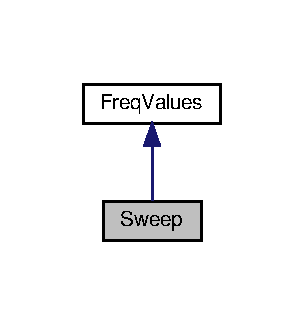
\includegraphics[width=146pt]{structSweep__inherit__graph}
\end{center}
\end{figure}


Collaboration diagram for Sweep\+:\nopagebreak
\begin{figure}[H]
\begin{center}
\leavevmode
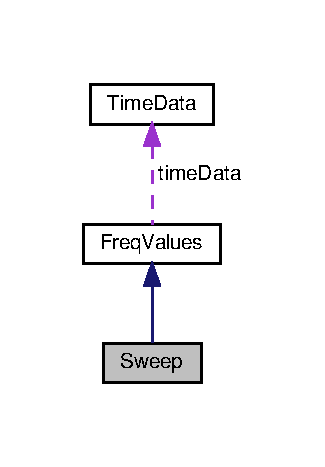
\includegraphics[width=156pt]{structSweep__coll__graph}
\end{center}
\end{figure}
\subsection*{Public Member Functions}
\begin{DoxyCompactItemize}
\item 
\mbox{\Hypertarget{structSweep_a154d8154b44ffd83c26375ca8d688591}\label{structSweep_a154d8154b44ffd83c26375ca8d688591}} 
\hyperlink{structSweep_a154d8154b44ffd83c26375ca8d688591}{Sweep} ()
\begin{DoxyCompactList}\small\item\em The default constructor which calls the default constructor of {\itshape \hyperlink{structFreqValues}{Freq\+Values}} structure and set type to \char`\"{}sweep\char`\"{} and azimuth angle to zero. \end{DoxyCompactList}\item 
\mbox{\Hypertarget{structSweep_ae85ac9f2a48f93e3fc510118c7d67f7f}\label{structSweep_ae85ac9f2a48f93e3fc510118c7d67f7f}} 
\hyperlink{structSweep_ae85ac9f2a48f93e3fc510118c7d67f7f}{Sweep} (const \hyperlink{structFreqValues}{Freq\+Values} \&freq\+Values)
\begin{DoxyCompactList}\small\item\em A copy constructor which receives a {\itshape \hyperlink{structFreqValues}{Freq\+Values}} object. \end{DoxyCompactList}\item 
\mbox{\Hypertarget{structSweep_a0a4e0f72fe9051d35cb29953005463b3}\label{structSweep_a0a4e0f72fe9051d35cb29953005463b3}} 
\hyperlink{structSweep_a0a4e0f72fe9051d35cb29953005463b3}{Sweep} (const \hyperlink{structSweep}{Sweep} \&sweep)
\begin{DoxyCompactList}\small\item\em A copy constructor which receives a {\itshape \hyperlink{structSweep}{Sweep}} object. \end{DoxyCompactList}\item 
\mbox{\Hypertarget{structSweep_aa852ab0cf53dc52ec354649cf6cec31e}\label{structSweep_aa852ab0cf53dc52ec354649cf6cec31e}} 
void \hyperlink{structSweep_aa852ab0cf53dc52ec354649cf6cec31e}{Clear} ()
\begin{DoxyCompactList}\small\item\em The aim of this method is to clean the structure, i.\+e. to delete all data points, set azimuth angle to zero and clean polarization. \end{DoxyCompactList}\item 
\mbox{\Hypertarget{structSweep_ae20eba1adf7d9510a2433ce942b14007}\label{structSweep_ae20eba1adf7d9510a2433ce942b14007}} 
const \hyperlink{structSweep}{Sweep} \& \hyperlink{structSweep_ae20eba1adf7d9510a2433ce942b14007}{operator=} (const \hyperlink{structSweep}{Sweep} \&sweep)
\begin{DoxyCompactList}\small\item\em An overloading of the assignment operator adapted to this structure. \end{DoxyCompactList}\end{DoxyCompactItemize}
\subsection*{Public Attributes}
\begin{DoxyCompactItemize}
\item 
\mbox{\Hypertarget{structSweep_a1400ee785843eba210c37a8f7e24c941}\label{structSweep_a1400ee785843eba210c37a8f7e24c941}} 
float \hyperlink{structSweep_a1400ee785843eba210c37a8f7e24c941}{azimuth\+Angle}
\begin{DoxyCompactList}\small\item\em The azimuth position (or angle) of the antenna when the sweep was captured. \end{DoxyCompactList}\item 
std\+::string \hyperlink{structSweep_a3484c258fdff60e1c109df92a1ba9ae7}{polarization}
\end{DoxyCompactItemize}
\subsection*{Friends}
\begin{DoxyCompactItemize}
\item 
\mbox{\Hypertarget{structSweep_a29420e86f220ed305794c8e560059bbc}\label{structSweep_a29420e86f220ed305794c8e560059bbc}} 
\hyperlink{structSweep}{Sweep} \hyperlink{structSweep_a29420e86f220ed305794c8e560059bbc}{operator-\/} (const \hyperlink{structSweep}{Sweep} \&argument)
\begin{DoxyCompactList}\small\item\em An overloading of the unary operator -\/ which negates a {\itshape \hyperlink{structSweep}{Sweep}} object. \end{DoxyCompactList}\item 
\mbox{\Hypertarget{structSweep_a96391241f10ea728ee36b62f6c35d604}\label{structSweep_a96391241f10ea728ee36b62f6c35d604}} 
\hyperlink{structSweep}{Sweep} \hyperlink{structSweep_a96391241f10ea728ee36b62f6c35d604}{operator+} (const \hyperlink{structSweep}{Sweep} \&lhs, const \hyperlink{structSweep}{Sweep} \&rhs)
\begin{DoxyCompactList}\small\item\em An overloading of operator + which calculates the sum of two objects of structure {\itshape \hyperlink{structSweep}{Sweep}}. \end{DoxyCompactList}\item 
\mbox{\Hypertarget{structSweep_ab372b814f572937b3f0cef31752994b9}\label{structSweep_ab372b814f572937b3f0cef31752994b9}} 
\hyperlink{structSweep}{Sweep} \hyperlink{structSweep_ab372b814f572937b3f0cef31752994b9}{operator+} (const \hyperlink{structSweep}{Sweep} \&lhs, const std\+::vector$<$ float $>$ \&rhs)
\begin{DoxyCompactList}\small\item\em An overloading of operator + which calculates the sum of a {\itshape \hyperlink{structSweep}{Sweep}} object and a {\ttfamily std\+::vector$<$float$>$} container, in that order. \end{DoxyCompactList}\item 
\mbox{\Hypertarget{structSweep_a770d2ac63866693c821c99cbfe2b2c9a}\label{structSweep_a770d2ac63866693c821c99cbfe2b2c9a}} 
\hyperlink{structSweep}{Sweep} \hyperlink{structSweep_a770d2ac63866693c821c99cbfe2b2c9a}{operator+} (const std\+::vector$<$ float $>$ \&lhs, const \hyperlink{structSweep}{Sweep} \&rhs)
\begin{DoxyCompactList}\small\item\em An overloading of operator + which calculates the sum of a {\ttfamily std\+::vector$<$float$>$} container and a {\itshape \hyperlink{structSweep}{Sweep}} object, in that order. \end{DoxyCompactList}\item 
\mbox{\Hypertarget{structSweep_a5d6fad874c778ae77a10b57446a0bd93}\label{structSweep_a5d6fad874c778ae77a10b57446a0bd93}} 
\hyperlink{structSweep}{Sweep} \hyperlink{structSweep_a5d6fad874c778ae77a10b57446a0bd93}{operator+} (const \hyperlink{structSweep}{Sweep} \&lhs, const \hyperlink{structFreqValues}{Freq\+Values} \&rhs)
\begin{DoxyCompactList}\small\item\em An overloading of operator + which calculates the sum of a {\itshape \hyperlink{structSweep}{Sweep}} object and a {\itshape \hyperlink{structFreqValues}{Freq\+Values}} object, in that order. \end{DoxyCompactList}\item 
\mbox{\Hypertarget{structSweep_ae8dce428f848644d0a68cc8309f88ebf}\label{structSweep_ae8dce428f848644d0a68cc8309f88ebf}} 
\hyperlink{structSweep}{Sweep} \hyperlink{structSweep_ae8dce428f848644d0a68cc8309f88ebf}{operator+} (const \hyperlink{structSweep}{Sweep} \&lhs, const float rhs)
\begin{DoxyCompactList}\small\item\em An overloading of operator + which calculates the sum of a {\itshape \hyperlink{structSweep}{Sweep}} object and a {\itshape float} value, in that order. \end{DoxyCompactList}\item 
\mbox{\Hypertarget{structSweep_ac0d73d5e8e3aab8f87c9815588b66821}\label{structSweep_ac0d73d5e8e3aab8f87c9815588b66821}} 
\hyperlink{structSweep}{Sweep} \hyperlink{structSweep_ac0d73d5e8e3aab8f87c9815588b66821}{operator+} (const float lhs, const \hyperlink{structSweep}{Sweep} \&rhs)
\begin{DoxyCompactList}\small\item\em An overloading of operator + which calculates the sum of a {\itshape float} value and a {\itshape \hyperlink{structSweep}{Sweep}} object, in that order. \end{DoxyCompactList}\item 
\mbox{\Hypertarget{structSweep_a8f704b31d015e4d81d25d3fceca1e2f1}\label{structSweep_a8f704b31d015e4d81d25d3fceca1e2f1}} 
\hyperlink{structSweep}{Sweep} \hyperlink{structSweep_a8f704b31d015e4d81d25d3fceca1e2f1}{operator-\/} (const \hyperlink{structSweep}{Sweep} \&lhs, const \hyperlink{structSweep}{Sweep} \&rhs)
\begin{DoxyCompactList}\small\item\em An overloading of operator -\/ which calculates the subtraction of two objects of structure {\itshape \hyperlink{structSweep}{Sweep}}. \end{DoxyCompactList}\item 
\mbox{\Hypertarget{structSweep_a8b2585969a3c379f744b662fb3bea749}\label{structSweep_a8b2585969a3c379f744b662fb3bea749}} 
\hyperlink{structSweep}{Sweep} \hyperlink{structSweep_a8b2585969a3c379f744b662fb3bea749}{operator-\/} (const \hyperlink{structSweep}{Sweep} \&lhs, const std\+::vector$<$ float $>$ \&rhs)
\begin{DoxyCompactList}\small\item\em An overloading of operator -\/ which calculates the subtraction of a {\itshape \hyperlink{structSweep}{Sweep}} object and a {\ttfamily std\+::vector$<$float$>$} container, in that order. \end{DoxyCompactList}\item 
\mbox{\Hypertarget{structSweep_a840a49afd7973b4b3d1020e15c4c9819}\label{structSweep_a840a49afd7973b4b3d1020e15c4c9819}} 
\hyperlink{structSweep}{Sweep} \hyperlink{structSweep_a840a49afd7973b4b3d1020e15c4c9819}{operator-\/} (const std\+::vector$<$ float $>$ \&lhs, const \hyperlink{structSweep}{Sweep} \&rhs)
\begin{DoxyCompactList}\small\item\em An overloading of operator -\/ which calculates the subtraction of a {\ttfamily std\+::vector$<$float$>$} container and a {\itshape \hyperlink{structSweep}{Sweep}} object, in that order. \end{DoxyCompactList}\item 
\mbox{\Hypertarget{structSweep_a124ea929f6dba249bd4d6bf5476ab621}\label{structSweep_a124ea929f6dba249bd4d6bf5476ab621}} 
\hyperlink{structSweep}{Sweep} \hyperlink{structSweep_a124ea929f6dba249bd4d6bf5476ab621}{operator-\/} (const \hyperlink{structSweep}{Sweep} \&lhs, const \hyperlink{structFreqValues}{Freq\+Values} \&rhs)
\begin{DoxyCompactList}\small\item\em An overloading of operator -\/ which calculates the subtraction of a {\itshape \hyperlink{structSweep}{Sweep}} object and a {\itshape \hyperlink{structFreqValues}{Freq\+Values}} object, in that order. \end{DoxyCompactList}\item 
\mbox{\Hypertarget{structSweep_a4739da92a36e5f8f17b0be140dd327f6}\label{structSweep_a4739da92a36e5f8f17b0be140dd327f6}} 
\hyperlink{structSweep}{Sweep} \hyperlink{structSweep_a4739da92a36e5f8f17b0be140dd327f6}{operator$\ast$} (const \hyperlink{structSweep}{Sweep} \&lhs, const \hyperlink{structSweep}{Sweep} \&rhs)
\begin{DoxyCompactList}\small\item\em An overloading of operator $\ast$ which multiplies two objects of structure {\itshape \hyperlink{structSweep}{Sweep}}. \end{DoxyCompactList}\item 
\mbox{\Hypertarget{structSweep_a12c1f3e5e4869781ca7d90a50f334606}\label{structSweep_a12c1f3e5e4869781ca7d90a50f334606}} 
\hyperlink{structSweep}{Sweep} \hyperlink{structSweep_a12c1f3e5e4869781ca7d90a50f334606}{operator$\ast$} (const \hyperlink{structSweep}{Sweep} \&lhs, const float rhs)
\begin{DoxyCompactList}\small\item\em An overloading of operator $\ast$ which multiplies a {\itshape \hyperlink{structSweep}{Sweep}} object and a {\itshape float} value, in that order. \end{DoxyCompactList}\item 
\mbox{\Hypertarget{structSweep_ad4aac4ab6e7ea49d5bc9ebfa83eb07be}\label{structSweep_ad4aac4ab6e7ea49d5bc9ebfa83eb07be}} 
\hyperlink{structSweep}{Sweep} \hyperlink{structSweep_ad4aac4ab6e7ea49d5bc9ebfa83eb07be}{operator$\ast$} (const float lhs, const \hyperlink{structSweep}{Sweep} \&rhs)
\begin{DoxyCompactList}\small\item\em An overloading of operator $\ast$ which multiplies a {\itshape float} value and a {\itshape \hyperlink{structSweep}{Sweep}} object, in that order. \end{DoxyCompactList}\item 
\mbox{\Hypertarget{structSweep_a3e230f15cb1119940203a1a452676b74}\label{structSweep_a3e230f15cb1119940203a1a452676b74}} 
\hyperlink{structSweep}{Sweep} \hyperlink{structSweep_a3e230f15cb1119940203a1a452676b74}{operator/} (const \hyperlink{structSweep}{Sweep} \&lhs, const \hyperlink{structSweep}{Sweep} \&rhs)
\begin{DoxyCompactList}\small\item\em An overloading of operator / which calculates the division between two objects of structure {\itshape \hyperlink{structSweep}{Sweep}}. \end{DoxyCompactList}\item 
\mbox{\Hypertarget{structSweep_a73694ded6e7ba41c367ca5f0934cbc2c}\label{structSweep_a73694ded6e7ba41c367ca5f0934cbc2c}} 
\hyperlink{structSweep}{Sweep} \hyperlink{structSweep_a73694ded6e7ba41c367ca5f0934cbc2c}{operator/} (const \hyperlink{structSweep}{Sweep} \&lhs, const float rhs)
\begin{DoxyCompactList}\small\item\em An overloading of operator / which calculates the division between a {\itshape \hyperlink{structSweep}{Sweep}} object and a {\itshape float} value, in that order. \end{DoxyCompactList}\item 
\mbox{\Hypertarget{structSweep_abe3c133bf246f7faebcfda286c5e1448}\label{structSweep_abe3c133bf246f7faebcfda286c5e1448}} 
\hyperlink{structSweep}{Sweep} \hyperlink{structSweep_abe3c133bf246f7faebcfda286c5e1448}{operator/} (const float lhs, const \hyperlink{structSweep}{Sweep} \&rhs)
\begin{DoxyCompactList}\small\item\em An overloading of operator / which calculates the division between a {\itshape float} value and a {\itshape \hyperlink{structSweep}{Sweep}} object, in that order. \end{DoxyCompactList}\item 
\mbox{\Hypertarget{structSweep_a37df38f37b1cf6a6bfb18f44b706d308}\label{structSweep_a37df38f37b1cf6a6bfb18f44b706d308}} 
\hyperlink{structSweep}{Sweep} \hyperlink{structSweep_a37df38f37b1cf6a6bfb18f44b706d308}{log10} (const \hyperlink{structSweep}{Sweep} \&argument)
\begin{DoxyCompactList}\small\item\em An overloading of function {\ttfamily \hyperlink{structSweep_a37df38f37b1cf6a6bfb18f44b706d308}{log10()}} adapted to receive an argument of type {\itshape \hyperlink{structSweep}{Sweep}}. \end{DoxyCompactList}\item 
\mbox{\Hypertarget{structSweep_a09ee88cfc9b28e6ec344eea1a2817ea9}\label{structSweep_a09ee88cfc9b28e6ec344eea1a2817ea9}} 
\hyperlink{structSweep}{Sweep} \hyperlink{structSweep_a09ee88cfc9b28e6ec344eea1a2817ea9}{pow} (const \hyperlink{structSweep}{Sweep} \&base, const float exponent)
\begin{DoxyCompactList}\small\item\em An overloading of function {\ttfamily \hyperlink{structSweep_a09ee88cfc9b28e6ec344eea1a2817ea9}{pow()}} adapted to receive an argument of type {\itshape \hyperlink{structSweep}{Sweep}} as base and an argument of type {\itshape float} as exponent. \end{DoxyCompactList}\item 
\mbox{\Hypertarget{structSweep_a879ae44efd2611562d05b90b24099e70}\label{structSweep_a879ae44efd2611562d05b90b24099e70}} 
\hyperlink{structSweep}{Sweep} \hyperlink{structSweep_a879ae44efd2611562d05b90b24099e70}{pow} (const float base, const \hyperlink{structSweep}{Sweep} \&exponent)
\begin{DoxyCompactList}\small\item\em An overloading of function {\ttfamily \hyperlink{structSweep_a09ee88cfc9b28e6ec344eea1a2817ea9}{pow()}} adapted to receive an argument of type {\itshape float} as base and an argument of type {\itshape \hyperlink{structSweep}{Sweep}} as exponent. \end{DoxyCompactList}\end{DoxyCompactItemize}


\subsection{Detailed Description}
The aim of this structure is to store the data points of a sweep obtained with the spectrum analyzer in a determined azimuth position, with a specific polarization. 

\subsection{Member Data Documentation}
\mbox{\Hypertarget{structSweep_a3484c258fdff60e1c109df92a1ba9ae7}\label{structSweep_a3484c258fdff60e1c109df92a1ba9ae7}} 
\index{Sweep@{Sweep}!polarization@{polarization}}
\index{polarization@{polarization}!Sweep@{Sweep}}
\subsubsection{\texorpdfstring{polarization}{polarization}}
{\footnotesize\ttfamily std\+::string Sweep\+::polarization}

The antenna polarization when the sweep was captured. 

The documentation for this struct was generated from the following file\+:\begin{DoxyCompactItemize}
\item 
\hyperlink{Basics_8h}{Basics.\+h}\end{DoxyCompactItemize}

\hypertarget{classSweepBuilder}{}\section{Sweep\+Builder Class Reference}
\label{classSweepBuilder}\index{Sweep\+Builder@{Sweep\+Builder}}


The aim of class {\itshape \hyperlink{classSweepBuilder}{Sweep\+Builder}} is to build the complete sweep from the individual sweep points which are delivered by the Spectran Interface.  




{\ttfamily \#include $<$Spectran.\+h$>$}

\subsection*{Public Member Functions}
\begin{DoxyCompactItemize}
\item 
\hyperlink{classSweepBuilder_a41b1ecbd8c74953fe0ad5bfbf03be667}{Sweep\+Builder} (\hyperlink{classSpectranInterface}{Spectran\+Interface} \&interf)
\begin{DoxyCompactList}\small\item\em The \hyperlink{classSweepBuilder}{Sweep\+Builder} class\textquotesingle{}s constructor. \end{DoxyCompactList}\item 
\mbox{\Hypertarget{classSweepBuilder_aa1be2613794ac488f3bf6c0b722c48d3}\label{classSweepBuilder_aa1be2613794ac488f3bf6c0b722c48d3}} 
\hyperlink{classSweepBuilder_aa1be2613794ac488f3bf6c0b722c48d3}{$\sim$\+Sweep\+Builder} ()
\begin{DoxyCompactList}\small\item\em The \hyperlink{classSweepBuilder}{Sweep\+Builder} class\textquotesingle{}s destructor. \end{DoxyCompactList}\item 
const \hyperlink{structSweep}{Sweep} \& \hyperlink{classSweepBuilder_ae8893395594bbf68873d33e3e7a0d192}{Capture\+Sweep} (\hyperlink{structBandParameters}{Band\+Parameters} \&band\+Param)
\begin{DoxyCompactList}\small\item\em The aim of this method is to capture one entire sweep from the spectrum analyzer through the Spectran Interface and returns this one. \end{DoxyCompactList}\item 
\mbox{\Hypertarget{classSweepBuilder_a5b7e3e8d18afb651927be8ea6e7ef1e1}\label{classSweepBuilder_a5b7e3e8d18afb651927be8ea6e7ef1e1}} 
const \hyperlink{structSweep}{Sweep} \& \hyperlink{classSweepBuilder_a5b7e3e8d18afb651927be8ea6e7ef1e1}{Get\+Sweep} () const
\begin{DoxyCompactList}\small\item\em This method returns the last captured sweep, as a {\itshape \hyperlink{structSweep}{Sweep}} structure. \end{DoxyCompactList}\end{DoxyCompactItemize}


\subsection{Detailed Description}
The aim of class {\itshape \hyperlink{classSweepBuilder}{Sweep\+Builder}} is to build the complete sweep from the individual sweep points which are delivered by the Spectran Interface. 

\subsection{Constructor \& Destructor Documentation}
\mbox{\Hypertarget{classSweepBuilder_a41b1ecbd8c74953fe0ad5bfbf03be667}\label{classSweepBuilder_a41b1ecbd8c74953fe0ad5bfbf03be667}} 
\index{Sweep\+Builder@{Sweep\+Builder}!Sweep\+Builder@{Sweep\+Builder}}
\index{Sweep\+Builder@{Sweep\+Builder}!Sweep\+Builder@{Sweep\+Builder}}
\subsubsection{\texorpdfstring{Sweep\+Builder()}{SweepBuilder()}}
{\footnotesize\ttfamily Sweep\+Builder\+::\+Sweep\+Builder (\begin{DoxyParamCaption}\item[{\hyperlink{classSpectranInterface}{Spectran\+Interface} \&}]{interf }\end{DoxyParamCaption})\hspace{0.3cm}{\ttfamily [inline]}}



The \hyperlink{classSweepBuilder}{Sweep\+Builder} class\textquotesingle{}s constructor. 


\begin{DoxyParams}[1]{Parameters}
\mbox{\tt in}  & {\em interf} & A reference to the unique {\itshape \hyperlink{classSpectranInterface}{Spectran\+Interface}} object, which is responsible for the communication with the spectrum analyzer. \\
\hline
\end{DoxyParams}


\subsection{Member Function Documentation}
\mbox{\Hypertarget{classSweepBuilder_ae8893395594bbf68873d33e3e7a0d192}\label{classSweepBuilder_ae8893395594bbf68873d33e3e7a0d192}} 
\index{Sweep\+Builder@{Sweep\+Builder}!Capture\+Sweep@{Capture\+Sweep}}
\index{Capture\+Sweep@{Capture\+Sweep}!Sweep\+Builder@{Sweep\+Builder}}
\subsubsection{\texorpdfstring{Capture\+Sweep()}{CaptureSweep()}}
{\footnotesize\ttfamily const \hyperlink{structSweep}{Sweep} \& Sweep\+Builder\+::\+Capture\+Sweep (\begin{DoxyParamCaption}\item[{\hyperlink{structBandParameters}{Band\+Parameters} \&}]{band\+Param }\end{DoxyParamCaption})}



The aim of this method is to capture one entire sweep from the spectrum analyzer through the Spectran Interface and returns this one. 

The method receives a {\itshape \hyperlink{structBandParameters}{Band\+Parameters}} structure, where the parameters of the current frequency band are stored, and it uses this structure to check if the frequency values are coherent and it corrects the number of sweep points of the structure.

First, the method sends a command to reset the current sweep, it waits a moment and then it enables the streaming of sweep points. Later, the method enters in a loop where each sweep point is captured and inserted in the {\ttfamily std\+::map} container. That kind of container are ordered and unique-\/key, so automatically the container orders the sweep points, taking into account the frequency, and it does not allow to insert two points with the same frequency. When that happens, the container states that and the loop finishes. Later, the number of sweep points is checked and stored in the given {\itshape \hyperlink{structBandParameters}{Band\+Parameters}} structure, the streaming of sweep points is disabled and, finally, the sweep is moved to a {\itshape \hyperlink{structSweep}{Sweep}} structure, which is more optimum to perform mathematical operations, and this structure is returned. 
\begin{DoxyParams}{Parameters}
{\em band\+Param} & \mbox{[}in,out\mbox{]} The parameters of the current frequency band. \\
\hline
\end{DoxyParams}


The documentation for this class was generated from the following files\+:\begin{DoxyCompactItemize}
\item 
\hyperlink{Spectran_8h}{Spectran.\+h}\item 
Sweep\+Builder.\+cpp\end{DoxyCompactItemize}

\hypertarget{classSweepReply}{}\section{Sweep\+Reply Class Reference}
\label{classSweepReply}\index{Sweep\+Reply@{Sweep\+Reply}}


This class derives from the base class {\itshape \hyperlink{classReply}{Reply}} and is intended to process in a better way replies with sweep points, i.\+e. {\itshape A\+M\+P\+F\+R\+E\+Q\+D\+AT} replies.  




{\ttfamily \#include $<$Spectran.\+h$>$}



Inheritance diagram for Sweep\+Reply\+:
\nopagebreak
\begin{figure}[H]
\begin{center}
\leavevmode
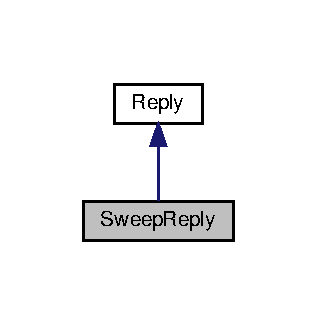
\includegraphics[width=152pt]{classSweepReply__inherit__graph}
\end{center}
\end{figure}


Collaboration diagram for Sweep\+Reply\+:
\nopagebreak
\begin{figure}[H]
\begin{center}
\leavevmode
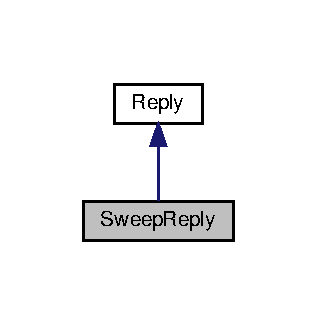
\includegraphics[width=152pt]{classSweepReply__coll__graph}
\end{center}
\end{figure}
\subsection*{Public Member Functions}
\begin{DoxyCompactItemize}
\item 
\hyperlink{classSweepReply_a27d588db63e7c9d5374cfbfc88d9bc4f}{Sweep\+Reply} ()
\begin{DoxyCompactList}\small\item\em The default constructor. \end{DoxyCompactList}\item 
\mbox{\Hypertarget{classSweepReply_a64fa7237d721d3dc95a06f145a0e7a7d}\label{classSweepReply_a64fa7237d721d3dc95a06f145a0e7a7d}} 
\hyperlink{classSweepReply_a64fa7237d721d3dc95a06f145a0e7a7d}{Sweep\+Reply} (const std\+::uint8\+\_\+t $\ast$bytes\+Ptr)
\begin{DoxyCompactList}\small\item\em A more complete constructor which allows to insert the received bytes of a reply. \end{DoxyCompactList}\item 
\mbox{\Hypertarget{classSweepReply_a513705c42bec154f66f75903813a5db1}\label{classSweepReply_a513705c42bec154f66f75903813a5db1}} 
void \hyperlink{classSweepReply_a513705c42bec154f66f75903813a5db1}{Prepare\+To} (const \hyperlink{classReply_aa873dec4817ed08a5212ec3ba2b5c807}{Reply\+Type} type, const \hyperlink{Spectran_8h_a0411392c90f0c8f0d8e44a4e94259276}{Spec\+Variable} variable=Spec\+Variable\+::\+U\+N\+I\+N\+I\+T\+I\+A\+L\+I\+Z\+ED)
\begin{DoxyCompactList}\small\item\em An overloading of the method {\ttfamily \hyperlink{classSweepReply_a513705c42bec154f66f75903813a5db1}{Prepare\+To()}} which just leave it without effect because this method has no sense in this derived class. \end{DoxyCompactList}\item 
void \hyperlink{classSweepReply_a8eff11f046d6cd2fb8c3987f889c5d11}{Insert\+Bytes} (const std\+::uint8\+\_\+t $\ast$data)
\begin{DoxyCompactList}\small\item\em An overloading of the corresponding method of the base class, which allows to insert the bytes of a A\+M\+P\+F\+R\+E\+Q\+D\+AT reply and to extract its data. \end{DoxyCompactList}\item 
\mbox{\Hypertarget{classSweepReply_a47ccfb08ddaa045ad170ce3583548ff2}\label{classSweepReply_a47ccfb08ddaa045ad170ce3583548ff2}} 
unsigned int \hyperlink{classSweepReply_a47ccfb08ddaa045ad170ce3583548ff2}{Get\+Timestamp} () const
\begin{DoxyCompactList}\small\item\em This method returns the timestamp of the corresponding sweep point. \end{DoxyCompactList}\item 
\mbox{\Hypertarget{classSweepReply_a68b46991b6ebf101ad8fa486831de9ed}\label{classSweepReply_a68b46991b6ebf101ad8fa486831de9ed}} 
std\+::uint\+\_\+least64\+\_\+t \hyperlink{classSweepReply_a68b46991b6ebf101ad8fa486831de9ed}{Get\+Frequency} () const
\begin{DoxyCompactList}\small\item\em This method returns the frequency value, which is in Hz. \end{DoxyCompactList}\item 
\mbox{\Hypertarget{classSweepReply_a77e184e7694b372de2100186cced425c}\label{classSweepReply_a77e184e7694b372de2100186cced425c}} 
float \hyperlink{classSweepReply_a77e184e7694b372de2100186cced425c}{Get\+Min\+Value} () const
\begin{DoxyCompactList}\small\item\em This method returns the minimum power value, in case of Min/\+Max detector is used, or the R\+MS power value, in case of R\+MS detector is used. Even, it could be a voltage or field strength value. \end{DoxyCompactList}\item 
\mbox{\Hypertarget{classSweepReply_af7332c7b0b73d2e3156b0da48ce78ff6}\label{classSweepReply_af7332c7b0b73d2e3156b0da48ce78ff6}} 
float \hyperlink{classSweepReply_af7332c7b0b73d2e3156b0da48ce78ff6}{Get\+Max\+Value} () const
\begin{DoxyCompactList}\small\item\em This method returns the maximum power value, in case of Min/\+Max detector is used, or the R\+MS power value, in case of R\+MS detector is used. Even, it could be a voltage or field strength value. \end{DoxyCompactList}\item 
\mbox{\Hypertarget{classSweepReply_a8273b23b929bfae3be36d2b061c7a793}\label{classSweepReply_a8273b23b929bfae3be36d2b061c7a793}} 
void \hyperlink{classSweepReply_a8273b23b929bfae3be36d2b061c7a793}{Clear} ()
\begin{DoxyCompactList}\small\item\em The aim of this method is to clear the class attributes. \end{DoxyCompactList}\item 
const \hyperlink{classSweepReply}{Sweep\+Reply} \& \hyperlink{classSweepReply_a37bfa46a9b437720ba551dd68875eeaa}{operator=} (const \hyperlink{classSweepReply}{Sweep\+Reply} \&another\+Reply)
\begin{DoxyCompactList}\small\item\em An overloading of the assignment operator, adapted to this class. \end{DoxyCompactList}\end{DoxyCompactItemize}
\subsection*{Additional Inherited Members}


\subsection{Detailed Description}
This class derives from the base class {\itshape \hyperlink{classReply}{Reply}} and is intended to process in a better way replies with sweep points, i.\+e. {\itshape A\+M\+P\+F\+R\+E\+Q\+D\+AT} replies. 

The purpose of this class is to handle the {\itshape A\+M\+P\+F\+R\+E\+Q\+D\+AT} replies which carry the sweep points. These specific replies need to be handled in a more complex way, so to simplify the base class ,which handles the others replies, a different class was made with the specific methods to extract the data from the A\+M\+P\+F\+R\+E\+Q\+D\+AT replies. 

\subsection{Constructor \& Destructor Documentation}
\mbox{\Hypertarget{classSweepReply_a27d588db63e7c9d5374cfbfc88d9bc4f}\label{classSweepReply_a27d588db63e7c9d5374cfbfc88d9bc4f}} 
\index{Sweep\+Reply@{Sweep\+Reply}!Sweep\+Reply@{Sweep\+Reply}}
\index{Sweep\+Reply@{Sweep\+Reply}!Sweep\+Reply@{Sweep\+Reply}}
\subsubsection{\texorpdfstring{Sweep\+Reply()}{SweepReply()}}
{\footnotesize\ttfamily Sweep\+Reply\+::\+Sweep\+Reply (\begin{DoxyParamCaption}{ }\end{DoxyParamCaption})}



The default constructor. 

This constructor clears the class attributes and calls the {\itshape \hyperlink{classReply}{Reply}} constructor with an argument to set the reply type to A\+M\+P\+F\+R\+E\+Q\+D\+AT. 

\subsection{Member Function Documentation}
\mbox{\Hypertarget{classSweepReply_a8eff11f046d6cd2fb8c3987f889c5d11}\label{classSweepReply_a8eff11f046d6cd2fb8c3987f889c5d11}} 
\index{Sweep\+Reply@{Sweep\+Reply}!Insert\+Bytes@{Insert\+Bytes}}
\index{Insert\+Bytes@{Insert\+Bytes}!Sweep\+Reply@{Sweep\+Reply}}
\subsubsection{\texorpdfstring{Insert\+Bytes()}{InsertBytes()}}
{\footnotesize\ttfamily void Sweep\+Reply\+::\+Insert\+Bytes (\begin{DoxyParamCaption}\item[{const std\+::uint8\+\_\+t $\ast$}]{data }\end{DoxyParamCaption})\hspace{0.3cm}{\ttfamily [virtual]}}



An overloading of the corresponding method of the base class, which allows to insert the bytes of a A\+M\+P\+F\+R\+E\+Q\+D\+AT reply and to extract its data. 

This method extracts the timestamp, frequency value and power values of a A\+M\+P\+F\+R\+E\+Q\+D\+AT reply. 
\begin{DoxyParams}[1]{Parameters}
\mbox{\tt in}  & {\em data} & A pointer to the bytes which contains the timestamp and the frequency and power values. \\
\hline
\end{DoxyParams}
Timestamp extraction\+: this value is received as a 4-\/byte unsigned integer and it represents the count of a internal timer of the spectrum analyzer. The timer period is approximately 3.\+5 nS and it is a 32-\/bit timer.

Frequency extraction\+: this value is received as a 4-\/byte unsigned integer in Hz/10 and it is stored as an unsigned integer in Hz.

Min/\+R\+MS power extraction\+: this value is received as a 4-\/byte floating point value, measured in d\+Bm. Even, it could be a voltage value or a field strength value.

Max/\+R\+MS power extraction\+: this value is received as a 4-\/bytes floating point value, measured in d\+Bm. Even, it could be a voltage value or a field strength value. 

Reimplemented from \hyperlink{classReply_a005fb1894b469cc16e69bf93fed967af}{Reply}.

\mbox{\Hypertarget{classSweepReply_a37bfa46a9b437720ba551dd68875eeaa}\label{classSweepReply_a37bfa46a9b437720ba551dd68875eeaa}} 
\index{Sweep\+Reply@{Sweep\+Reply}!operator=@{operator=}}
\index{operator=@{operator=}!Sweep\+Reply@{Sweep\+Reply}}
\subsubsection{\texorpdfstring{operator=()}{operator=()}}
{\footnotesize\ttfamily const \hyperlink{classSweepReply}{Sweep\+Reply} \& Sweep\+Reply\+::operator= (\begin{DoxyParamCaption}\item[{const \hyperlink{classSweepReply}{Sweep\+Reply} \&}]{another\+Reply }\end{DoxyParamCaption})}



An overloading of the assignment operator, adapted to this class. 


\begin{DoxyParams}[1]{Parameters}
\mbox{\tt in}  & {\em another\+Reply} & A {\itshape \hyperlink{classReply}{Reply}} object which is given to copy its attributes. \\
\hline
\end{DoxyParams}


The documentation for this class was generated from the following files\+:\begin{DoxyCompactItemize}
\item 
/home/new-\/mauro/eclipse-\/cdt/workspace/\+R\+F\+I\+M\+S\+\_\+\+C\+A\+R\+T/src/\hyperlink{Spectran_8h}{Spectran.\+h}\item 
/home/new-\/mauro/eclipse-\/cdt/workspace/\+R\+F\+I\+M\+S\+\_\+\+C\+A\+R\+T/src/\hyperlink{Reply_8cpp}{Reply.\+cpp}\end{DoxyCompactItemize}

\hypertarget{structTimeData}{}\section{Time\+Data Struct Reference}
\label{structTimeData}\index{Time\+Data@{Time\+Data}}


This structure is intended to store data related to {\itshape date} and {\itshape time} and to perform some operations with that data.  




{\ttfamily \#include $<$Basics.\+h$>$}

\subsection*{Public Member Functions}
\begin{DoxyCompactItemize}
\item 
\mbox{\Hypertarget{structTimeData_a4be51d0cd0dce3b91ce449b6c995a9e9}\label{structTimeData_a4be51d0cd0dce3b91ce449b6c995a9e9}} 
\hyperlink{structTimeData_a4be51d0cd0dce3b91ce449b6c995a9e9}{Time\+Data} ()
\begin{DoxyCompactList}\small\item\em The class\textquotesingle{} constructor which clear all attributes, i.\+e. set date and time as 00-\/00-\/00\+T00\+:00\+:00. \end{DoxyCompactList}\item 
\mbox{\Hypertarget{structTimeData_af0454b54d768d6b21267b3692dae4d3d}\label{structTimeData_af0454b54d768d6b21267b3692dae4d3d}} 
\hyperlink{structTimeData_af0454b54d768d6b21267b3692dae4d3d}{Time\+Data} (const \hyperlink{structTimeData}{Time\+Data} \&time\+Data)
\begin{DoxyCompactList}\small\item\em The class\textquotesingle{} copy constructor. \end{DoxyCompactList}\item 
\mbox{\Hypertarget{structTimeData_a78640fbf87e59255e08836b6779ec5c0}\label{structTimeData_a78640fbf87e59255e08836b6779ec5c0}} 
std\+::string \hyperlink{structTimeData_a78640fbf87e59255e08836b6779ec5c0}{Get\+Date} () const
\begin{DoxyCompactList}\small\item\em A method to get the date as a {\ttfamily std\+::string} \end{DoxyCompactList}\item 
\mbox{\Hypertarget{structTimeData_a6810621b9bd2289b697a7cd7b1799515}\label{structTimeData_a6810621b9bd2289b697a7cd7b1799515}} 
std\+::string \hyperlink{structTimeData_a6810621b9bd2289b697a7cd7b1799515}{Get\+Time} () const
\begin{DoxyCompactList}\small\item\em A method to get the time as a {\ttfamily std\+::string} \end{DoxyCompactList}\item 
\mbox{\Hypertarget{structTimeData_a06956ece691807dc69e4fe6add2bd423}\label{structTimeData_a06956ece691807dc69e4fe6add2bd423}} 
std\+::string \hyperlink{structTimeData_a06956ece691807dc69e4fe6add2bd423}{Get\+Timestamp} () const
\begin{DoxyCompactList}\small\item\em A method to get a timestamp as a {\ttfamily std\+::string} with the format D\+D-\/\+M\+M-\/\+Y\+Y\+Y\+Y\+T\+HH\+:MM\+:SS. \end{DoxyCompactList}\item 
\mbox{\Hypertarget{structTimeData_ac4a84f214fbaeaac5fa77df2c68bad79}\label{structTimeData_ac4a84f214fbaeaac5fa77df2c68bad79}} 
void \hyperlink{structTimeData_ac4a84f214fbaeaac5fa77df2c68bad79}{Set\+Date} (const std\+::string \&date)
\begin{DoxyCompactList}\small\item\em This method is intended to set just the date. \end{DoxyCompactList}\item 
\mbox{\Hypertarget{structTimeData_a79c359b6aa1d5362065105d0e6b2f657}\label{structTimeData_a79c359b6aa1d5362065105d0e6b2f657}} 
void \hyperlink{structTimeData_a79c359b6aa1d5362065105d0e6b2f657}{Set\+Time} (const std\+::string \&time)
\begin{DoxyCompactList}\small\item\em This method is intended to set just the time. \end{DoxyCompactList}\item 
\mbox{\Hypertarget{structTimeData_a753d18acb1fdebbde3e910e2462b4073}\label{structTimeData_a753d18acb1fdebbde3e910e2462b4073}} 
void \hyperlink{structTimeData_a753d18acb1fdebbde3e910e2462b4073}{Set\+Timestamp} (const std\+::string \&timestamp)
\begin{DoxyCompactList}\small\item\em This method is intended to modify all attributes, giving these as a timestamp. \end{DoxyCompactList}\item 
\mbox{\Hypertarget{structTimeData_ad204062485d50c24aad1d4b41a582bd8}\label{structTimeData_ad204062485d50c24aad1d4b41a582bd8}} 
void \hyperlink{structTimeData_ad204062485d50c24aad1d4b41a582bd8}{Turn\+Back\+Days} (const unsigned int days)
\begin{DoxyCompactList}\small\item\em This method allows to turn a time point back a specified number of days. \end{DoxyCompactList}\item 
\mbox{\Hypertarget{structTimeData_a43ba78733adf4369e4c8c89db1819772}\label{structTimeData_a43ba78733adf4369e4c8c89db1819772}} 
const \hyperlink{structTimeData}{Time\+Data} \& \hyperlink{structTimeData_a43ba78733adf4369e4c8c89db1819772}{operator=} (const \hyperlink{structTimeData}{Time\+Data} \&another\+Time\+Data)
\begin{DoxyCompactList}\small\item\em An overloading of the assignmetn operator. \end{DoxyCompactList}\item 
\mbox{\Hypertarget{structTimeData_af1071330f0fadc98a5e08d41a8436907}\label{structTimeData_af1071330f0fadc98a5e08d41a8436907}} 
void \hyperlink{structTimeData_af1071330f0fadc98a5e08d41a8436907}{Clear} ()
\begin{DoxyCompactList}\small\item\em A method to clear all attributes, i.\+e. it set the object as 00-\/00-\/00\+T00\+:00\+:00. \end{DoxyCompactList}\end{DoxyCompactItemize}
\subsection*{Public Attributes}
\begin{DoxyCompactItemize}
\item 
\mbox{\Hypertarget{structTimeData_a457ba435747cdc51aa3c9213dc75e916}\label{structTimeData_a457ba435747cdc51aa3c9213dc75e916}} 
unsigned int \hyperlink{structTimeData_a457ba435747cdc51aa3c9213dc75e916}{year}
\begin{DoxyCompactList}\small\item\em This variable stores the year, taking into account the estimated birth of Jesus. \end{DoxyCompactList}\item 
\mbox{\Hypertarget{structTimeData_a54ec81ff233394814cb837c41cd3ea0b}\label{structTimeData_a54ec81ff233394814cb837c41cd3ea0b}} 
unsigned int \hyperlink{structTimeData_a54ec81ff233394814cb837c41cd3ea0b}{month}
\begin{DoxyCompactList}\small\item\em This variable stores the month as a number that can be between 1 and 12. \end{DoxyCompactList}\item 
\mbox{\Hypertarget{structTimeData_aee725dc9551cd482534c155a168b3d60}\label{structTimeData_aee725dc9551cd482534c155a168b3d60}} 
unsigned int \hyperlink{structTimeData_aee725dc9551cd482534c155a168b3d60}{day}
\begin{DoxyCompactList}\small\item\em This variable stores the day as a number that can be between 1 and 31, taking into account the corresponding month. \end{DoxyCompactList}\item 
\mbox{\Hypertarget{structTimeData_a989207381ecc5a4c744bd06bf1091c63}\label{structTimeData_a989207381ecc5a4c744bd06bf1091c63}} 
unsigned int \hyperlink{structTimeData_a989207381ecc5a4c744bd06bf1091c63}{hour}
\begin{DoxyCompactList}\small\item\em This variable stores the hours as a number that can be between 0 and 23. \end{DoxyCompactList}\item 
\mbox{\Hypertarget{structTimeData_ac22938d020a988bebae2493b118b9df2}\label{structTimeData_ac22938d020a988bebae2493b118b9df2}} 
unsigned int \hyperlink{structTimeData_ac22938d020a988bebae2493b118b9df2}{minute}
\begin{DoxyCompactList}\small\item\em This variable stores the minutes as a number that can be between 0 and 59. \end{DoxyCompactList}\item 
\mbox{\Hypertarget{structTimeData_ac17cd0725bea21f3be277d2c9a00e3d8}\label{structTimeData_ac17cd0725bea21f3be277d2c9a00e3d8}} 
unsigned int \hyperlink{structTimeData_ac17cd0725bea21f3be277d2c9a00e3d8}{second}
\begin{DoxyCompactList}\small\item\em This variable stores the seconds as a number that can be between 0 and 59. \end{DoxyCompactList}\end{DoxyCompactItemize}
\subsection*{Friends}
\begin{DoxyCompactItemize}
\item 
\mbox{\Hypertarget{structTimeData_a05ed1f021fd859fd0507d8ec74de5afd}\label{structTimeData_a05ed1f021fd859fd0507d8ec74de5afd}} 
bool \hyperlink{structTimeData_a05ed1f021fd859fd0507d8ec74de5afd}{operator$<$} (const \hyperlink{structTimeData}{Time\+Data} \&lhs, const \hyperlink{structTimeData}{Time\+Data} \&rhs)
\begin{DoxyCompactList}\small\item\em An overloading of the operator $<$ to compare two \hyperlink{structTimeData}{Time\+Data} objects as the first one lesser than the second one. \end{DoxyCompactList}\item 
\mbox{\Hypertarget{structTimeData_a6ba5c50a9564dae90072889e68cc8a42}\label{structTimeData_a6ba5c50a9564dae90072889e68cc8a42}} 
bool \hyperlink{structTimeData_a6ba5c50a9564dae90072889e68cc8a42}{operator$>$} (const \hyperlink{structTimeData}{Time\+Data} \&lhs, const \hyperlink{structTimeData}{Time\+Data} \&rhs)
\begin{DoxyCompactList}\small\item\em An overloading of the operator $>$ to compare two \hyperlink{structTimeData}{Time\+Data} objects as the first one bigger than the second one. \end{DoxyCompactList}\item 
\mbox{\Hypertarget{structTimeData_a77e7e3db1d21909c98eb40309a3ac989}\label{structTimeData_a77e7e3db1d21909c98eb40309a3ac989}} 
bool \hyperlink{structTimeData_a77e7e3db1d21909c98eb40309a3ac989}{operator==} (const \hyperlink{structTimeData}{Time\+Data} \&lhs, const \hyperlink{structTimeData}{Time\+Data} \&rhs)
\begin{DoxyCompactList}\small\item\em An overloading of the operator == to compare two \hyperlink{structTimeData}{Time\+Data} objects as equal. \end{DoxyCompactList}\end{DoxyCompactItemize}


\subsection{Detailed Description}
This structure is intended to store data related to {\itshape date} and {\itshape time} and to perform some operations with that data. 

This structure can store time data (hour, minute and second) and date data (year, month and date) which are obtained from a G\+PS receiver. It can offer just the date as a string, or just the time as a string or even can build a {\itshape timestamp} with a specific format\+: D\+D-\/\+M\+M-\/\+Y\+Y\+Y\+Y\+T\+HH\+:MM\+:SS. Also it can take a date and time and turn that back a specific number of days taking into account the {\itshape gregorian} calendar. An object of this class can even be compared as equal to, less than or bigger than another object of the same class. 

The documentation for this struct was generated from the following file\+:\begin{DoxyCompactItemize}
\item 
\hyperlink{Basics_8h}{Basics.\+h}\end{DoxyCompactItemize}

\chapter{File Documentation}
\hypertarget{AntennaPositioning_8h}{}\section{/home/new-\/mauro/eclipse-\/cdt/workspace/\+R\+F\+I\+M\+S\+\_\+\+C\+A\+R\+T/src/\+Antenna\+Positioning.h File Reference}
\label{AntennaPositioning_8h}\index{/home/new-\/mauro/eclipse-\/cdt/workspace/\+R\+F\+I\+M\+S\+\_\+\+C\+A\+R\+T/src/\+Antenna\+Positioning.\+h@{/home/new-\/mauro/eclipse-\/cdt/workspace/\+R\+F\+I\+M\+S\+\_\+\+C\+A\+R\+T/src/\+Antenna\+Positioning.\+h}}


This file contains the declarations of classes \hyperlink{classAntennaPositioner}{Antenna\+Positioner} and \hyperlink{classGPSInterface}{G\+P\+S\+Interface}.  


{\ttfamily \#include \char`\"{}Basics.\+h\char`\"{}}\newline
{\ttfamily \#include $<$nmea.\+h$>$}\newline
{\ttfamily \#include $<$nmea/gprmc.\+h$>$}\newline
{\ttfamily \#include $<$nmea/gpgga.\+h$>$}\newline
{\ttfamily \#include $<$ftd2xx.\+h$>$}\newline
{\ttfamily \#include $<$dirent.\+h$>$}\newline
Include dependency graph for Antenna\+Positioning.\+h\+:\nopagebreak
\begin{figure}[H]
\begin{center}
\leavevmode
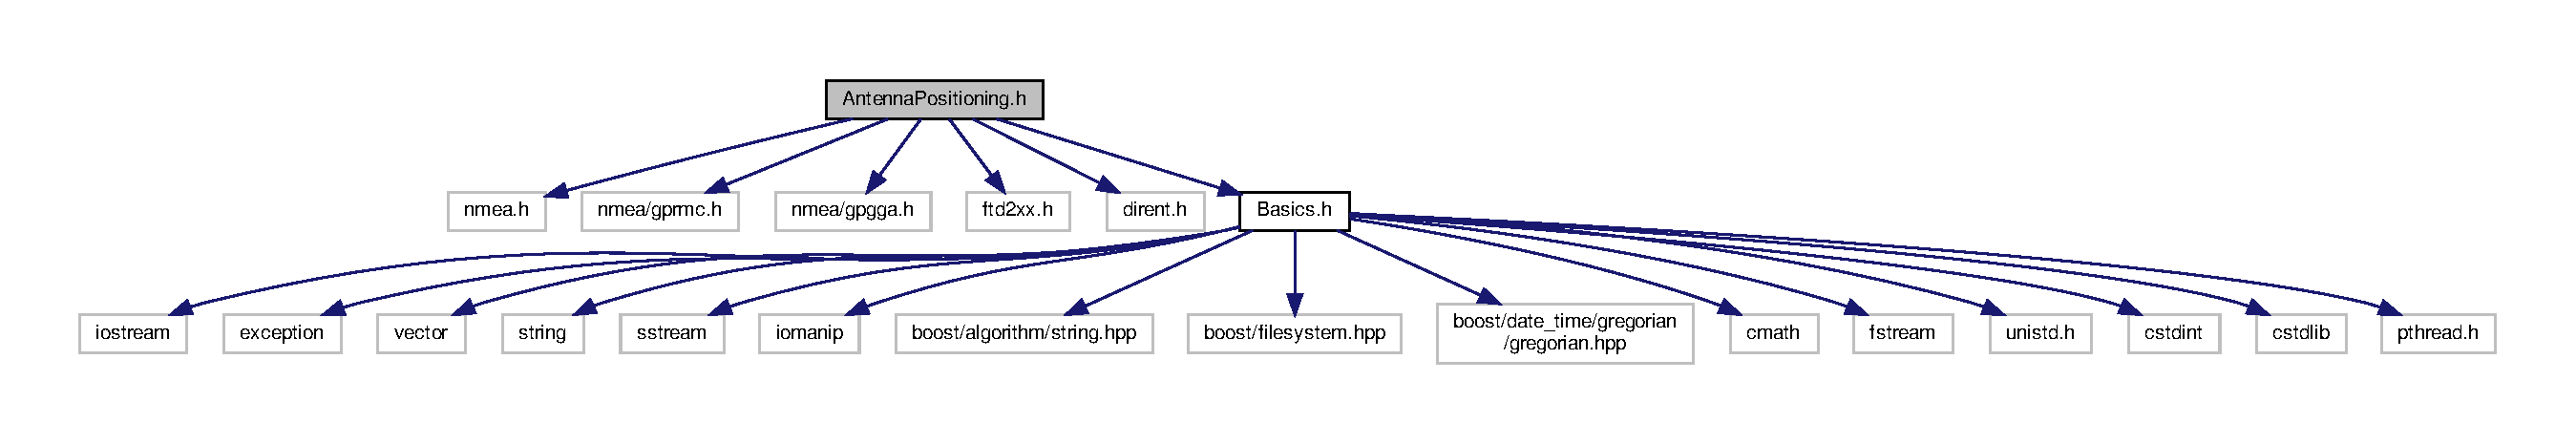
\includegraphics[width=350pt]{AntennaPositioning_8h__incl}
\end{center}
\end{figure}
This graph shows which files directly or indirectly include this file\+:\nopagebreak
\begin{figure}[H]
\begin{center}
\leavevmode
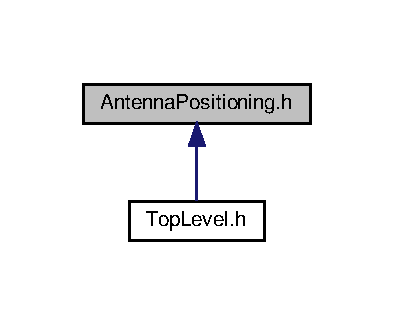
\includegraphics[width=350pt]{AntennaPositioning_8h__dep__incl}
\end{center}
\end{figure}
\subsection*{Classes}
\begin{DoxyCompactItemize}
\item 
struct \hyperlink{structData3D}{Data3D}
\begin{DoxyCompactList}\small\item\em A structure intended to save the the values of the 3d sensors which are integrated in the G\+PS receiver. \end{DoxyCompactList}\item 
struct \hyperlink{structGPSCoordinates}{G\+P\+S\+Coordinates}
\begin{DoxyCompactList}\small\item\em A structure which saves the G\+PS coordinates. \end{DoxyCompactList}\item 
class \hyperlink{classGPSInterface}{G\+P\+S\+Interface}
\begin{DoxyCompactList}\small\item\em The class {\itshape G\+P\+S\+Interace} is intended to establish the communication with the Aaronia G\+PS receiver, to request and capture messages from this one and extract useful data from the messages. \end{DoxyCompactList}\item 
class \hyperlink{classAntennaPositioner}{Antenna\+Positioner}
\begin{DoxyCompactList}\small\item\em The aim of the class {\itshape \hyperlink{classAntennaPositioner}{Antenna\+Positioner}} is to handle the antenna positioning system. \end{DoxyCompactList}\end{DoxyCompactItemize}
\subsection*{Enumerations}
\begin{DoxyCompactItemize}
\item 
\mbox{\Hypertarget{AntennaPositioning_8h_a55887c7bc32d70c0308472ff4de3e282}\label{AntennaPositioning_8h_a55887c7bc32d70c0308472ff4de3e282}} 
enum \hyperlink{AntennaPositioning_8h_a55887c7bc32d70c0308472ff4de3e282}{Polarization} \+: char \{ {\bfseries H\+O\+R\+I\+Z\+O\+N\+T\+AL}, 
{\bfseries V\+E\+R\+T\+I\+C\+AL}, 
{\bfseries U\+N\+K\+N\+O\+WN}
 \}\begin{DoxyCompactList}\small\item\em An enumeration which contains the possible states of the antenna polarization\+: H\+O\+R\+I\+Z\+O\+N\+T\+AL, V\+E\+R\+T\+I\+C\+AL or U\+N\+K\+N\+O\+WN. \end{DoxyCompactList}
\end{DoxyCompactItemize}


\subsection{Detailed Description}
This file contains the declarations of classes \hyperlink{classAntennaPositioner}{Antenna\+Positioner} and \hyperlink{classGPSInterface}{G\+P\+S\+Interface}. 

These classes are responsible for the positioning of the antenna, which can rotate its azimuth angle and its polarization. To model these rotations it were used the Cardan angles (or nautical angles)\+: the \char`\"{}yaw\char`\"{} angle which represents the heading, the \char`\"{}pitch\char`\"{} angle which represents the elevation and the \char`\"{}roll\char`\"{} angle which models the bank angle. The yaw angle is used to represent the antenna\textquotesingle{}s azimuth angle, the roll angle is used to represent the antenna polarization and the pitch angle is not used. 
\begin{DoxyImage}
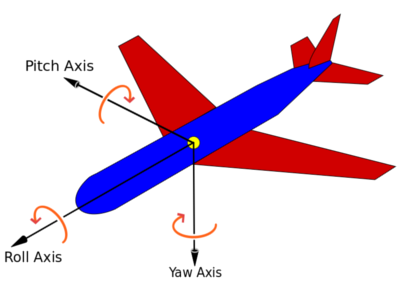
\includegraphics[width=10cm]{cardan_angles}
\doxyfigcaption{The Cardan or nautical angles}
\end{DoxyImage}
 Moreover, the class \hyperlink{classGPSInterface}{G\+P\+S\+Interface} allows to get data related with time and date, elevation (based on pressure), ambient pressure, among other things.

Also, several structures are defined here which store data related with the mentioned classes. \begin{DoxyAuthor}{Author}
Mauro Diamantino 
\end{DoxyAuthor}

\hypertarget{Basics_8cpp}{}\section{/home/new-\/mauro/eclipse-\/cdt/workspace/\+R\+F\+I\+M\+S\+\_\+\+C\+A\+R\+T/src/\+Basics.cpp File Reference}
\label{Basics_8cpp}\index{/home/new-\/mauro/eclipse-\/cdt/workspace/\+R\+F\+I\+M\+S\+\_\+\+C\+A\+R\+T/src/\+Basics.\+cpp@{/home/new-\/mauro/eclipse-\/cdt/workspace/\+R\+F\+I\+M\+S\+\_\+\+C\+A\+R\+T/src/\+Basics.\+cpp}}


This file contains the definitions of the functions and classes\textquotesingle{} methods which have been declared in file \hyperlink{Basics_8h}{Basics.\+h}.  


{\ttfamily \#include \char`\"{}Basics.\+h\char`\"{}}\newline
Include dependency graph for Basics.\+cpp\+:\nopagebreak
\begin{figure}[H]
\begin{center}
\leavevmode
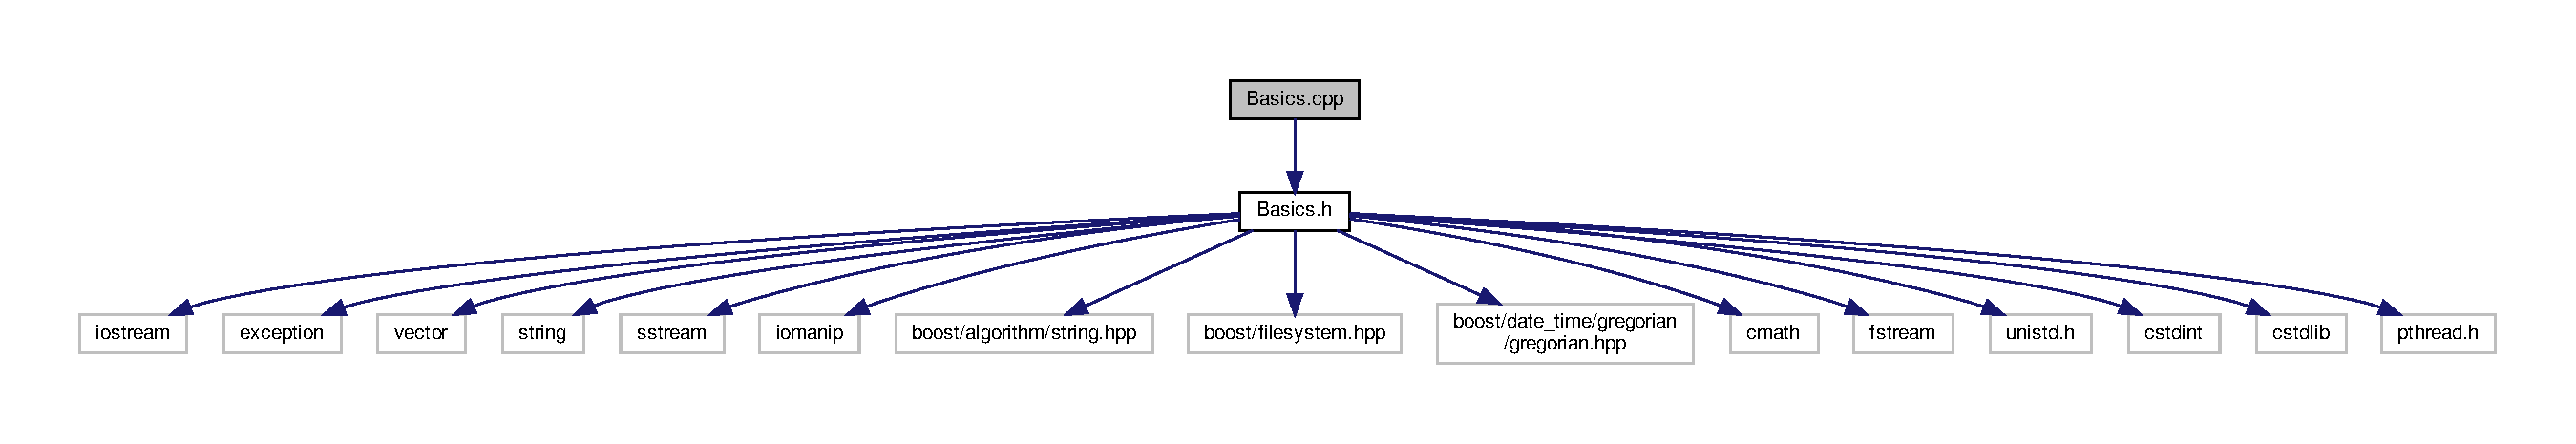
\includegraphics[width=350pt]{Basics_8cpp__incl}
\end{center}
\end{figure}
\subsection*{Functions}
\begin{DoxyCompactItemize}
\item 
bool \hyperlink{Basics_8cpp_ab0cf00620947abc90fbfe36db36f8fc7}{approximately\+Equal} (float a, float b)
\begin{DoxyCompactList}\small\item\em Function intended to compare floating-\/point numbers as approximately equal, taking into account the floating-\/point rounding errors. \end{DoxyCompactList}\item 
bool \hyperlink{Basics_8cpp_adee734e43e4a9a5f4b9f610ccdd3f8e0}{approximately\+Equal} (std\+::vector$<$ float $>$ vectorA, std\+::vector$<$ float $>$ vectorB)
\begin{DoxyCompactList}\small\item\em Function intended to compare {\ttfamily std\+::vector$<$float$>$} containers as approximately equal, taking into account the floating-\/point rounding errors. \end{DoxyCompactList}\item 
\mbox{\Hypertarget{Basics_8cpp_abe6b1466ff5e3b09c33ca5dc9fc81c5a}\label{Basics_8cpp_abe6b1466ff5e3b09c33ca5dc9fc81c5a}} 
void \hyperlink{Basics_8cpp_abe6b1466ff5e3b09c33ca5dc9fc81c5a}{Wait\+For\+Key} ()
\begin{DoxyCompactList}\small\item\em This function stop the execution up to any key is pressed by the user and it was used for debugging purpose. \end{DoxyCompactList}\item 
std\+::vector$<$ float $>$ \hyperlink{Basics_8cpp_ac744212c600f3f610807ec4add576822}{operator-\/} (const std\+::vector$<$ float $>$ \&\hyperlink{Spectran_8h_a16fa8eb91a19fde7a399d85c521f63fd}{vect})
\begin{DoxyCompactList}\small\item\em An overloading of unary operator -\/ which negates the elements of a {\ttfamily std\+::vector$<$float$>$} container. \end{DoxyCompactList}\item 
\mbox{\Hypertarget{Basics_8cpp_adb434b11769fc3a9acd409f2fe534395}\label{Basics_8cpp_adb434b11769fc3a9acd409f2fe534395}} 
void \hyperlink{Basics_8cpp_adb434b11769fc3a9acd409f2fe534395}{Initialize\+G\+P\+IO} ()
\begin{DoxyCompactList}\small\item\em This function initializes all G\+P\+IO pins which are used for the input and output signals, in the way it is described in structure {\itshape pi\+Pins}. \end{DoxyCompactList}\item 
\mbox{\Hypertarget{Basics_8cpp_a37d643c013d8e020715ec625553673e7}\label{Basics_8cpp_a37d643c013d8e020715ec625553673e7}} 
void \hyperlink{Basics_8cpp_a37d643c013d8e020715ec625553673e7}{Turn\+Off\+Leds} ()
\begin{DoxyCompactList}\small\item\em The aim of this function is to turn all L\+E\+Ds off. \end{DoxyCompactList}\item 
void \hyperlink{Basics_8cpp_a2f7418278fcdac50f5c6a73744f8013c}{Turn\+On\+Front\+End} ()
\begin{DoxyCompactList}\small\item\em The aim of this function is to turn on the RF front-\/end elements in a sequential manner, from the spectrum analyzer to the antenna.. \end{DoxyCompactList}\item 
void \hyperlink{Basics_8cpp_a5ffe8b7dfe9c6702ed65b2b8b47bc3e1}{Turn\+Off\+Front\+End} ()
\begin{DoxyCompactList}\small\item\em The aim of this function is to turn off the RF front-\/end elements in a sequential manner, from the antenna to the spectrum analyzer. \end{DoxyCompactList}\item 
\mbox{\Hypertarget{Basics_8cpp_ae964ff8411b4fdcaf65cb5529aea4bef}\label{Basics_8cpp_ae964ff8411b4fdcaf65cb5529aea4bef}} 
void \hyperlink{Basics_8cpp_ae964ff8411b4fdcaf65cb5529aea4bef}{Print\+Help} ()
\begin{DoxyCompactList}\small\item\em This function prints in the {\ttfamily stdout} a message whit a software description and the descriptions of its arguments. \end{DoxyCompactList}\item 
bool \hyperlink{Basics_8cpp_abab505eef94a08a9092f916c62637071}{Process\+Main\+Arguments} (int argc, char $\ast$argv\mbox{[}$\,$\mbox{]})
\begin{DoxyCompactList}\small\item\em This function process the software\textquotesingle{}s arguments, which define the behavior of this one. \end{DoxyCompactList}\end{DoxyCompactItemize}


\subsection{Detailed Description}
This file contains the definitions of the functions and classes\textquotesingle{} methods which have been declared in file \hyperlink{Basics_8h}{Basics.\+h}. 

\begin{DoxyAuthor}{Author}
Mauro Diamantino 
\end{DoxyAuthor}


\subsection{Function Documentation}
\mbox{\Hypertarget{Basics_8cpp_ab0cf00620947abc90fbfe36db36f8fc7}\label{Basics_8cpp_ab0cf00620947abc90fbfe36db36f8fc7}} 
\index{Basics.\+cpp@{Basics.\+cpp}!approximately\+Equal@{approximately\+Equal}}
\index{approximately\+Equal@{approximately\+Equal}!Basics.\+cpp@{Basics.\+cpp}}
\subsubsection{\texorpdfstring{approximately\+Equal()}{approximatelyEqual()}\hspace{0.1cm}{\footnotesize\ttfamily [1/2]}}
{\footnotesize\ttfamily bool approximately\+Equal (\begin{DoxyParamCaption}\item[{float}]{a,  }\item[{float}]{b }\end{DoxyParamCaption})}



Function intended to compare floating-\/point numbers as approximately equal, taking into account the floating-\/point rounding errors. 

This function was copied from this \href{https://www.learncpp.com/cpp-tutorial/35-relational-operators-comparisons/}{\tt link}, but it was modified. It is based in the Knuth’s algorithm but it uses two epsilons, an absolute epsilon (A\+B\+S\+\_\+\+E\+P\+S\+I\+L\+ON) which is very small and is intended to compare near-\/zero floating-\/point numbers and a relative epsilon (R\+E\+L\+\_\+\+E\+P\+S\+I\+L\+ON, which is a percentage of the biggest operand) to compare the rest of the floating-\/point numbers. The function returns true if the difference between a and b is less than A\+B\+S\+\_\+\+E\+P\+S\+I\+L\+ON, or within R\+E\+L\+\_\+\+E\+P\+S\+I\+L\+ON percent of the larger of a and b. 
\begin{DoxyParams}[1]{Parameters}
\mbox{\tt in}  & {\em a} & The left-\/hand side argument. \\
\hline
\mbox{\tt in}  & {\em b} & The right-\/hand side argument. \\
\hline
\end{DoxyParams}
\mbox{\Hypertarget{Basics_8cpp_adee734e43e4a9a5f4b9f610ccdd3f8e0}\label{Basics_8cpp_adee734e43e4a9a5f4b9f610ccdd3f8e0}} 
\index{Basics.\+cpp@{Basics.\+cpp}!approximately\+Equal@{approximately\+Equal}}
\index{approximately\+Equal@{approximately\+Equal}!Basics.\+cpp@{Basics.\+cpp}}
\subsubsection{\texorpdfstring{approximately\+Equal()}{approximatelyEqual()}\hspace{0.1cm}{\footnotesize\ttfamily [2/2]}}
{\footnotesize\ttfamily bool approximately\+Equal (\begin{DoxyParamCaption}\item[{std\+::vector$<$ float $>$}]{vectorA,  }\item[{std\+::vector$<$ float $>$}]{vectorB }\end{DoxyParamCaption})}



Function intended to compare {\ttfamily std\+::vector$<$float$>$} containers as approximately equal, taking into account the floating-\/point rounding errors. 

This function is based on the function presented in this \href{https://www.learncpp.com/cpp-tutorial/35-relational-operators-comparisons/}{\tt link}.

It is based in the Knuth’s algorithm but it uses two epsilons, an absolute epsilon (A\+B\+S\+\_\+\+E\+P\+S\+I\+L\+ON) which is very small and is intended to compare near-\/zero floating-\/point numbers and a relative epsilon (R\+E\+L\+\_\+\+E\+P\+S\+I\+L\+ON, which is a percentage of the biggest operand) to compare the rest of the floating-\/point numbers. The function returns true if the difference between a and b is less than A\+B\+S\+\_\+\+E\+P\+S\+I\+L\+ON, or within R\+E\+L\+\_\+\+E\+P\+S\+I\+L\+ON percent of the larger of a and b. 
\begin{DoxyParams}[1]{Parameters}
\mbox{\tt in}  & {\em vectorA} & The left-\/hand side argument. \\
\hline
\mbox{\tt in}  & {\em vectorB} & The right-\/hand side argument. \\
\hline
\end{DoxyParams}
\mbox{\Hypertarget{Basics_8cpp_ac744212c600f3f610807ec4add576822}\label{Basics_8cpp_ac744212c600f3f610807ec4add576822}} 
\index{Basics.\+cpp@{Basics.\+cpp}!operator-\/@{operator-\/}}
\index{operator-\/@{operator-\/}!Basics.\+cpp@{Basics.\+cpp}}
\subsubsection{\texorpdfstring{operator-\/()}{operator-()}}
{\footnotesize\ttfamily std\+::vector$<$float$>$ operator-\/ (\begin{DoxyParamCaption}\item[{const std\+::vector$<$ float $>$ \&}]{vect }\end{DoxyParamCaption})}



An overloading of unary operator -\/ which negates the elements of a {\ttfamily std\+::vector$<$float$>$} container. 


\begin{DoxyParams}[1]{Parameters}
\mbox{\tt in}  & {\em vect} & A {\ttfamily std\+::vector$<$float$>$} container which must be negated. \\
\hline
\end{DoxyParams}
\mbox{\Hypertarget{Basics_8cpp_abab505eef94a08a9092f916c62637071}\label{Basics_8cpp_abab505eef94a08a9092f916c62637071}} 
\index{Basics.\+cpp@{Basics.\+cpp}!Process\+Main\+Arguments@{Process\+Main\+Arguments}}
\index{Process\+Main\+Arguments@{Process\+Main\+Arguments}!Basics.\+cpp@{Basics.\+cpp}}
\subsubsection{\texorpdfstring{Process\+Main\+Arguments()}{ProcessMainArguments()}}
{\footnotesize\ttfamily bool Process\+Main\+Arguments (\begin{DoxyParamCaption}\item[{int}]{argc,  }\item[{char $\ast$}]{argv\mbox{[}$\,$\mbox{]} }\end{DoxyParamCaption})}



This function process the software\textquotesingle{}s arguments, which define the behavior of this one. 

This function determines the values of the behavior flags (flag\+Cal\+Enabled, flag\+Plot, flag\+R\+FI, etc.) taking into account the arguments that were received and its values. The function returns a {\ttfamily true} value if the arguments were processed correctly and a {\ttfamily false} value if there was an argument which could not be recognized, and in that case it presents a message, in the {\ttfamily stdout}, explaining the correct use of the software arguments. 
\begin{DoxyParams}[1]{Parameters}
\mbox{\tt in}  & {\em argc} & The number of arguments that were received by the software. \\
\hline
\mbox{\tt in}  & {\em argv} & An array of C strings ({\ttfamily char$\ast$}) where each one is a software\textquotesingle{}s argument. \\
\hline
\end{DoxyParams}
\mbox{\Hypertarget{Basics_8cpp_a5ffe8b7dfe9c6702ed65b2b8b47bc3e1}\label{Basics_8cpp_a5ffe8b7dfe9c6702ed65b2b8b47bc3e1}} 
\index{Basics.\+cpp@{Basics.\+cpp}!Turn\+Off\+Front\+End@{Turn\+Off\+Front\+End}}
\index{Turn\+Off\+Front\+End@{Turn\+Off\+Front\+End}!Basics.\+cpp@{Basics.\+cpp}}
\subsubsection{\texorpdfstring{Turn\+Off\+Front\+End()}{TurnOffFrontEnd()}}
{\footnotesize\ttfamily void Turn\+Off\+Front\+End (\begin{DoxyParamCaption}{ }\end{DoxyParamCaption})}



The aim of this function is to turn off the RF front-\/end elements in a sequential manner, from the antenna to the spectrum analyzer. 

To turn off the RF front-\/end elements sequentially, this function begins ensuring the noise source is turned off, then it switches the input to that device, it waits 1 second, it turns the L\+N\+As off, it waits again 1 second and, finally, it turns the spectrum analyzer off. \mbox{\Hypertarget{Basics_8cpp_a2f7418278fcdac50f5c6a73744f8013c}\label{Basics_8cpp_a2f7418278fcdac50f5c6a73744f8013c}} 
\index{Basics.\+cpp@{Basics.\+cpp}!Turn\+On\+Front\+End@{Turn\+On\+Front\+End}}
\index{Turn\+On\+Front\+End@{Turn\+On\+Front\+End}!Basics.\+cpp@{Basics.\+cpp}}
\subsubsection{\texorpdfstring{Turn\+On\+Front\+End()}{TurnOnFrontEnd()}}
{\footnotesize\ttfamily void Turn\+On\+Front\+End (\begin{DoxyParamCaption}{ }\end{DoxyParamCaption})}



The aim of this function is to turn on the RF front-\/end elements in a sequential manner, from the spectrum analyzer to the antenna.. 

To turn on the RF front-\/end elements in a sequential manner, first, this function turns the spectrum analyzer on, then it waits 5 seconds, it turns the L\+N\+As on, it waits again but this time just 1 second and, finally, it switches the input to the antenna. 
\hypertarget{Basics_8h}{}\section{/home/new-\/mauro/eclipse-\/cdt/workspace/\+R\+F\+I\+M\+S\+\_\+\+C\+A\+R\+T/src/\+Basics.h File Reference}
\label{Basics_8h}\index{/home/new-\/mauro/eclipse-\/cdt/workspace/\+R\+F\+I\+M\+S\+\_\+\+C\+A\+R\+T/src/\+Basics.\+h@{/home/new-\/mauro/eclipse-\/cdt/workspace/\+R\+F\+I\+M\+S\+\_\+\+C\+A\+R\+T/src/\+Basics.\+h}}


This header file contains the declarations of the most basic and global entities which are used by many others entities.  


{\ttfamily \#include $<$iostream$>$}\newline
{\ttfamily \#include $<$exception$>$}\newline
{\ttfamily \#include $<$vector$>$}\newline
{\ttfamily \#include $<$string$>$}\newline
{\ttfamily \#include $<$sstream$>$}\newline
{\ttfamily \#include $<$iomanip$>$}\newline
{\ttfamily \#include $<$boost/algorithm/string.\+hpp$>$}\newline
{\ttfamily \#include $<$boost/filesystem.\+hpp$>$}\newline
{\ttfamily \#include $<$boost/date\+\_\+time/gregorian/gregorian.\+hpp$>$}\newline
{\ttfamily \#include $<$cmath$>$}\newline
{\ttfamily \#include $<$fstream$>$}\newline
{\ttfamily \#include $<$unistd.\+h$>$}\newline
{\ttfamily \#include $<$cstdint$>$}\newline
{\ttfamily \#include $<$cstdlib$>$}\newline
{\ttfamily \#include $<$pthread.\+h$>$}\newline
Include dependency graph for Basics.\+h\+:\nopagebreak
\begin{figure}[H]
\begin{center}
\leavevmode
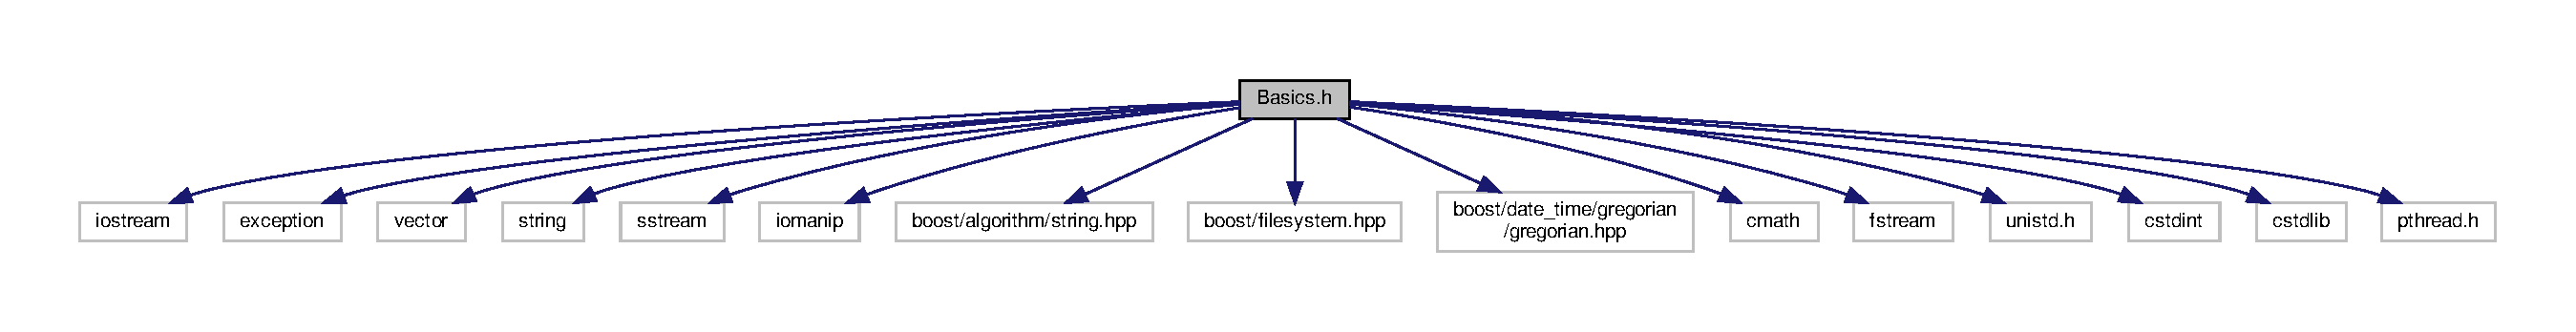
\includegraphics[width=350pt]{Basics_8h__incl}
\end{center}
\end{figure}
This graph shows which files directly or indirectly include this file\+:\nopagebreak
\begin{figure}[H]
\begin{center}
\leavevmode
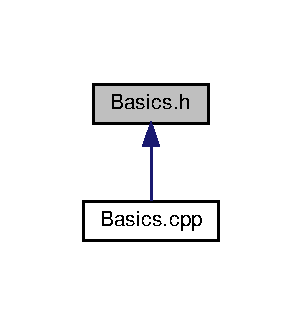
\includegraphics[width=350pt]{Basics_8h__dep__incl}
\end{center}
\end{figure}
\subsection*{Classes}
\begin{DoxyCompactItemize}
\item 
class \hyperlink{classCustomException}{Custom\+Exception}
\begin{DoxyCompactList}\small\item\em A class derived from standard class {\ttfamily std\+::exception}. \end{DoxyCompactList}\item 
struct \hyperlink{structTimeData}{Time\+Data}
\begin{DoxyCompactList}\small\item\em This structure is intended to store data related to {\itshape date} and {\itshape time} and to perform some operations with that data. \end{DoxyCompactList}\item 
struct \hyperlink{structFreqValues}{Freq\+Values}
\begin{DoxyCompactList}\small\item\em The aim of this structure is to store the curve of a determined parameter or variable versus the frequency, which is named a frequency curve here. \end{DoxyCompactList}\item 
struct \hyperlink{structSweep}{Sweep}
\begin{DoxyCompactList}\small\item\em The aim of this structure is to store the data points of a sweep obtained with the spectrum analyzer in a determined azimuth position, with a specific polarization. \end{DoxyCompactList}\item 
struct \hyperlink{structRFI}{R\+FI}
\begin{DoxyCompactList}\small\item\em The aim of this structure is to store the data related with the detected RF interference (\hyperlink{structRFI}{R\+FI})\+: frequency, power, azimuth angle, polarization, time, reference norm, etc. \end{DoxyCompactList}\item 
struct \hyperlink{structBandParameters}{Band\+Parameters}
\begin{DoxyCompactList}\small\item\em This structure is intended to store the parameters which are used to configure the spectrum analyzer in each frequency band. \end{DoxyCompactList}\end{DoxyCompactItemize}
\subsection*{Functions}
\begin{DoxyCompactItemize}
\item 
bool \hyperlink{Basics_8h_ab0cf00620947abc90fbfe36db36f8fc7}{approximately\+Equal} (float a, float b)
\begin{DoxyCompactList}\small\item\em Function intended to compare floating-\/point numbers as approximately equal, taking into account the floating-\/point rounding errors. \end{DoxyCompactList}\item 
bool \hyperlink{Basics_8h_adee734e43e4a9a5f4b9f610ccdd3f8e0}{approximately\+Equal} (std\+::vector$<$ float $>$ vectorA, std\+::vector$<$ float $>$ vectorB)
\begin{DoxyCompactList}\small\item\em Function intended to compare {\ttfamily std\+::vector$<$float$>$} containers as approximately equal, taking into account the floating-\/point rounding errors. \end{DoxyCompactList}\item 
std\+::vector$<$ float $>$ \hyperlink{Basics_8h_ac744212c600f3f610807ec4add576822}{operator-\/} (const std\+::vector$<$ float $>$ \&\hyperlink{Spectran_8h_a16fa8eb91a19fde7a399d85c521f63fd}{vect})
\begin{DoxyCompactList}\small\item\em An overloading of unary operator -\/ which negates the elements of a {\ttfamily std\+::vector$<$float$>$} container. \end{DoxyCompactList}\item 
\mbox{\Hypertarget{Basics_8h_abe6b1466ff5e3b09c33ca5dc9fc81c5a}\label{Basics_8h_abe6b1466ff5e3b09c33ca5dc9fc81c5a}} 
void \hyperlink{Basics_8h_abe6b1466ff5e3b09c33ca5dc9fc81c5a}{Wait\+For\+Key} ()
\begin{DoxyCompactList}\small\item\em This function stop the execution up to any key is pressed by the user and it was used for debugging purpose. \end{DoxyCompactList}\item 
\mbox{\Hypertarget{Basics_8h_adb434b11769fc3a9acd409f2fe534395}\label{Basics_8h_adb434b11769fc3a9acd409f2fe534395}} 
void \hyperlink{Basics_8h_adb434b11769fc3a9acd409f2fe534395}{Initialize\+G\+P\+IO} ()
\begin{DoxyCompactList}\small\item\em This function initializes all G\+P\+IO pins which are used for the input and output signals, in the way it is described in structure {\itshape pi\+Pins}. \end{DoxyCompactList}\item 
\mbox{\Hypertarget{Basics_8h_a37d643c013d8e020715ec625553673e7}\label{Basics_8h_a37d643c013d8e020715ec625553673e7}} 
void \hyperlink{Basics_8h_a37d643c013d8e020715ec625553673e7}{Turn\+Off\+Leds} ()
\begin{DoxyCompactList}\small\item\em The aim of this function is to turn all L\+E\+Ds off. \end{DoxyCompactList}\item 
void \hyperlink{Basics_8h_a2f7418278fcdac50f5c6a73744f8013c}{Turn\+On\+Front\+End} ()
\begin{DoxyCompactList}\small\item\em The aim of this function is to turn on the RF front-\/end elements in a sequential manner, from the spectrum analyzer to the antenna.. \end{DoxyCompactList}\item 
void \hyperlink{Basics_8h_a5ffe8b7dfe9c6702ed65b2b8b47bc3e1}{Turn\+Off\+Front\+End} ()
\begin{DoxyCompactList}\small\item\em The aim of this function is to turn off the RF front-\/end elements in a sequential manner, from the antenna to the spectrum analyzer. \end{DoxyCompactList}\item 
\mbox{\Hypertarget{Basics_8h_ae964ff8411b4fdcaf65cb5529aea4bef}\label{Basics_8h_ae964ff8411b4fdcaf65cb5529aea4bef}} 
void \hyperlink{Basics_8h_ae964ff8411b4fdcaf65cb5529aea4bef}{Print\+Help} ()
\begin{DoxyCompactList}\small\item\em This function prints in the {\ttfamily stdout} a message whit a software description and the descriptions of its arguments. \end{DoxyCompactList}\item 
bool \hyperlink{Basics_8h_abab505eef94a08a9092f916c62637071}{Process\+Main\+Arguments} (int argc, char $\ast$argv\mbox{[}$\,$\mbox{]})
\begin{DoxyCompactList}\small\item\em This function process the software\textquotesingle{}s arguments, which define the behavior of this one. \end{DoxyCompactList}\end{DoxyCompactItemize}
\subsection*{Variables}
\begin{DoxyCompactItemize}
\item 
\mbox{\Hypertarget{Basics_8h_a0423f4cb393331ce0b9f6b3a43adcaae}\label{Basics_8h_a0423f4cb393331ce0b9f6b3a43adcaae}} 
const std\+::string \hyperlink{Basics_8h_a0423f4cb393331ce0b9f6b3a43adcaae}{B\+A\+S\+E\+\_\+\+P\+A\+TH} = \char`\"{}/home/new-\/mauro/R\+F\+I\+MS-\/C\+A\+RT\char`\"{}
\begin{DoxyCompactList}\small\item\em This constant define the base path where there are the files and folders used by the software. \end{DoxyCompactList}\item 
\mbox{\Hypertarget{Basics_8h_a73be6649a1d91070309752a2fbcf5b8a}\label{Basics_8h_a73be6649a1d91070309752a2fbcf5b8a}} 
bool \hyperlink{Basics_8h_a73be6649a1d91070309752a2fbcf5b8a}{flag\+Cal\+Enabled}
\begin{DoxyCompactList}\small\item\em The declaration of an external flag which defines if the calibration of the RF front end must be done or not. \end{DoxyCompactList}\item 
\mbox{\Hypertarget{Basics_8h_a20c207881b1f505ca91715905e27bacb}\label{Basics_8h_a20c207881b1f505ca91715905e27bacb}} 
bool \hyperlink{Basics_8h_a20c207881b1f505ca91715905e27bacb}{flag\+Plot}
\begin{DoxyCompactList}\small\item\em The declaration of an external flag which defines if the software has to generate plots. \end{DoxyCompactList}\item 
\mbox{\Hypertarget{Basics_8h_a6f3cbd74619175fd2b8580b37587f825}\label{Basics_8h_a6f3cbd74619175fd2b8580b37587f825}} 
bool \hyperlink{Basics_8h_a6f3cbd74619175fd2b8580b37587f825}{flag\+Infinite\+Loop}
\begin{DoxyCompactList}\small\item\em The declaration of an external flag which defines if the software has to perform a finite number of measurement cycles or iterate infinitely. \end{DoxyCompactList}\item 
\mbox{\Hypertarget{Basics_8h_a816d4b897ea7e7b008ad3957e2203934}\label{Basics_8h_a816d4b897ea7e7b008ad3957e2203934}} 
bool \hyperlink{Basics_8h_a816d4b897ea7e7b008ad3957e2203934}{flag\+R\+FI}
\begin{DoxyCompactList}\small\item\em The declaration of an external flag which defines if the software has to perform \hyperlink{structRFI}{R\+FI} detection or not. \end{DoxyCompactList}\item 
\mbox{\Hypertarget{Basics_8h_a7616186dd32bbd21eb512dfdc580214c}\label{Basics_8h_a7616186dd32bbd21eb512dfdc580214c}} 
bool \hyperlink{Basics_8h_a7616186dd32bbd21eb512dfdc580214c}{flag\+Upload}
\begin{DoxyCompactList}\small\item\em The declaration of an external flag which defines if the software has to upload the measurements or not. \end{DoxyCompactList}\item 
unsigned int \hyperlink{Basics_8h_a4a22fc28d7ca5b183f4a901f4dafd4a6}{num\+Of\+Meas\+Cycles}
\begin{DoxyCompactList}\small\item\em The declaration of an external variable which stores the number of measurements cycles which left to be done. It is used when the user wishes a finite number of measurements cycles. \end{DoxyCompactList}\item 
\hyperlink{structRFI_a18cfa7d24274bbcd14acc6b513860cb0}{R\+F\+I\+::\+Thresholds\+Norm} \hyperlink{Basics_8h_a5fca012de3aeabad258f4f0fa6877334}{rfi\+Norm}
\begin{DoxyCompactList}\small\item\em The declaration of an external variable which saves the norm which defines the harmful interference levels\+: ska-\/mode1, ska-\/mode2, itu-\/ra769-\/2-\/vlbi. \end{DoxyCompactList}\end{DoxyCompactItemize}


\subsection{Detailed Description}
This header file contains the declarations of the most basic and global entities which are used by many others entities. 

This header file contains the declarations and definitions of the following\+:
\begin{DoxyItemize}
\item Preprocessor definitions ({\ttfamily define})\+: these elements define the blocks of code will be taking into account by the compiler, so the way the software will behave after the compilation and linking.
\item Global libraries, i.\+e. the libraries which are used by several functions and classes from different files.
\item Global constants and variables.
\item Global structures which are used to interchange data between different objects and functions.
\item Global structures which contain common data to all software\textquotesingle{}s entities.
\item A global class to handle exceptions.
\item Global functions which are used in several different places. \begin{DoxyAuthor}{Author}
Mauro Diamantino 
\end{DoxyAuthor}

\end{DoxyItemize}

\subsection{Function Documentation}
\mbox{\Hypertarget{Basics_8h_ab0cf00620947abc90fbfe36db36f8fc7}\label{Basics_8h_ab0cf00620947abc90fbfe36db36f8fc7}} 
\index{Basics.\+h@{Basics.\+h}!approximately\+Equal@{approximately\+Equal}}
\index{approximately\+Equal@{approximately\+Equal}!Basics.\+h@{Basics.\+h}}
\subsubsection{\texorpdfstring{approximately\+Equal()}{approximatelyEqual()}\hspace{0.1cm}{\footnotesize\ttfamily [1/2]}}
{\footnotesize\ttfamily bool approximately\+Equal (\begin{DoxyParamCaption}\item[{float}]{a,  }\item[{float}]{b }\end{DoxyParamCaption})}



Function intended to compare floating-\/point numbers as approximately equal, taking into account the floating-\/point rounding errors. 

This function was copied from this \href{https://www.learncpp.com/cpp-tutorial/35-relational-operators-comparisons/}{\tt link}, but it was modified. It is based in the Knuth’s algorithm but it uses two epsilons, an absolute epsilon (A\+B\+S\+\_\+\+E\+P\+S\+I\+L\+ON) which is very small and is intended to compare near-\/zero floating-\/point numbers and a relative epsilon (R\+E\+L\+\_\+\+E\+P\+S\+I\+L\+ON, which is a percentage of the biggest operand) to compare the rest of the floating-\/point numbers. The function returns true if the difference between a and b is less than A\+B\+S\+\_\+\+E\+P\+S\+I\+L\+ON, or within R\+E\+L\+\_\+\+E\+P\+S\+I\+L\+ON percent of the larger of a and b. 
\begin{DoxyParams}[1]{Parameters}
\mbox{\tt in}  & {\em a} & The left-\/hand side argument. \\
\hline
\mbox{\tt in}  & {\em b} & The right-\/hand side argument. \\
\hline
\end{DoxyParams}
\mbox{\Hypertarget{Basics_8h_adee734e43e4a9a5f4b9f610ccdd3f8e0}\label{Basics_8h_adee734e43e4a9a5f4b9f610ccdd3f8e0}} 
\index{Basics.\+h@{Basics.\+h}!approximately\+Equal@{approximately\+Equal}}
\index{approximately\+Equal@{approximately\+Equal}!Basics.\+h@{Basics.\+h}}
\subsubsection{\texorpdfstring{approximately\+Equal()}{approximatelyEqual()}\hspace{0.1cm}{\footnotesize\ttfamily [2/2]}}
{\footnotesize\ttfamily bool approximately\+Equal (\begin{DoxyParamCaption}\item[{std\+::vector$<$ float $>$}]{vectorA,  }\item[{std\+::vector$<$ float $>$}]{vectorB }\end{DoxyParamCaption})}



Function intended to compare {\ttfamily std\+::vector$<$float$>$} containers as approximately equal, taking into account the floating-\/point rounding errors. 

This function is based on the function presented in this \href{https://www.learncpp.com/cpp-tutorial/35-relational-operators-comparisons/}{\tt link}.

It is based in the Knuth’s algorithm but it uses two epsilons, an absolute epsilon (A\+B\+S\+\_\+\+E\+P\+S\+I\+L\+ON) which is very small and is intended to compare near-\/zero floating-\/point numbers and a relative epsilon (R\+E\+L\+\_\+\+E\+P\+S\+I\+L\+ON, which is a percentage of the biggest operand) to compare the rest of the floating-\/point numbers. The function returns true if the difference between a and b is less than A\+B\+S\+\_\+\+E\+P\+S\+I\+L\+ON, or within R\+E\+L\+\_\+\+E\+P\+S\+I\+L\+ON percent of the larger of a and b. 
\begin{DoxyParams}[1]{Parameters}
\mbox{\tt in}  & {\em vectorA} & The left-\/hand side argument. \\
\hline
\mbox{\tt in}  & {\em vectorB} & The right-\/hand side argument. \\
\hline
\end{DoxyParams}
\mbox{\Hypertarget{Basics_8h_ac744212c600f3f610807ec4add576822}\label{Basics_8h_ac744212c600f3f610807ec4add576822}} 
\index{Basics.\+h@{Basics.\+h}!operator-\/@{operator-\/}}
\index{operator-\/@{operator-\/}!Basics.\+h@{Basics.\+h}}
\subsubsection{\texorpdfstring{operator-\/()}{operator-()}}
{\footnotesize\ttfamily std\+::vector$<$float$>$ operator-\/ (\begin{DoxyParamCaption}\item[{const std\+::vector$<$ float $>$ \&}]{vect }\end{DoxyParamCaption})}



An overloading of unary operator -\/ which negates the elements of a {\ttfamily std\+::vector$<$float$>$} container. 


\begin{DoxyParams}[1]{Parameters}
\mbox{\tt in}  & {\em vect} & A {\ttfamily std\+::vector$<$float$>$} container which must be negated. \\
\hline
\end{DoxyParams}
\mbox{\Hypertarget{Basics_8h_abab505eef94a08a9092f916c62637071}\label{Basics_8h_abab505eef94a08a9092f916c62637071}} 
\index{Basics.\+h@{Basics.\+h}!Process\+Main\+Arguments@{Process\+Main\+Arguments}}
\index{Process\+Main\+Arguments@{Process\+Main\+Arguments}!Basics.\+h@{Basics.\+h}}
\subsubsection{\texorpdfstring{Process\+Main\+Arguments()}{ProcessMainArguments()}}
{\footnotesize\ttfamily bool Process\+Main\+Arguments (\begin{DoxyParamCaption}\item[{int}]{argc,  }\item[{char $\ast$}]{argv\mbox{[}$\,$\mbox{]} }\end{DoxyParamCaption})}



This function process the software\textquotesingle{}s arguments, which define the behavior of this one. 

This function determines the values of the behavior flags (flag\+Cal\+Enabled, flag\+Plot, flag\+R\+FI, etc.) taking into account the arguments that were received and its values. The function returns a {\ttfamily true} value if the arguments were processed correctly and a {\ttfamily false} value if there was an argument which could not be recognized, and in that case it presents a message, in the {\ttfamily stdout}, explaining the correct use of the software arguments. 
\begin{DoxyParams}[1]{Parameters}
\mbox{\tt in}  & {\em argc} & The number of arguments that were received by the software. \\
\hline
\mbox{\tt in}  & {\em argv} & An array of C strings ({\ttfamily char$\ast$}) where each one is a software\textquotesingle{}s argument. \\
\hline
\end{DoxyParams}
\mbox{\Hypertarget{Basics_8h_a5ffe8b7dfe9c6702ed65b2b8b47bc3e1}\label{Basics_8h_a5ffe8b7dfe9c6702ed65b2b8b47bc3e1}} 
\index{Basics.\+h@{Basics.\+h}!Turn\+Off\+Front\+End@{Turn\+Off\+Front\+End}}
\index{Turn\+Off\+Front\+End@{Turn\+Off\+Front\+End}!Basics.\+h@{Basics.\+h}}
\subsubsection{\texorpdfstring{Turn\+Off\+Front\+End()}{TurnOffFrontEnd()}}
{\footnotesize\ttfamily void Turn\+Off\+Front\+End (\begin{DoxyParamCaption}{ }\end{DoxyParamCaption})}



The aim of this function is to turn off the RF front-\/end elements in a sequential manner, from the antenna to the spectrum analyzer. 

To turn off the RF front-\/end elements sequentially, this function begins ensuring the noise source is turned off, then it switches the input to that device, it waits 1 second, it turns the L\+N\+As off, it waits again 1 second and, finally, it turns the spectrum analyzer off. \mbox{\Hypertarget{Basics_8h_a2f7418278fcdac50f5c6a73744f8013c}\label{Basics_8h_a2f7418278fcdac50f5c6a73744f8013c}} 
\index{Basics.\+h@{Basics.\+h}!Turn\+On\+Front\+End@{Turn\+On\+Front\+End}}
\index{Turn\+On\+Front\+End@{Turn\+On\+Front\+End}!Basics.\+h@{Basics.\+h}}
\subsubsection{\texorpdfstring{Turn\+On\+Front\+End()}{TurnOnFrontEnd()}}
{\footnotesize\ttfamily void Turn\+On\+Front\+End (\begin{DoxyParamCaption}{ }\end{DoxyParamCaption})}



The aim of this function is to turn on the RF front-\/end elements in a sequential manner, from the spectrum analyzer to the antenna.. 

To turn on the RF front-\/end elements in a sequential manner, first, this function turns the spectrum analyzer on, then it waits 5 seconds, it turns the L\+N\+As on, it waits again but this time just 1 second and, finally, it switches the input to the antenna. 

\subsection{Variable Documentation}
\mbox{\Hypertarget{Basics_8h_a4a22fc28d7ca5b183f4a901f4dafd4a6}\label{Basics_8h_a4a22fc28d7ca5b183f4a901f4dafd4a6}} 
\index{Basics.\+h@{Basics.\+h}!num\+Of\+Meas\+Cycles@{num\+Of\+Meas\+Cycles}}
\index{num\+Of\+Meas\+Cycles@{num\+Of\+Meas\+Cycles}!Basics.\+h@{Basics.\+h}}
\subsubsection{\texorpdfstring{num\+Of\+Meas\+Cycles}{numOfMeasCycles}}
{\footnotesize\ttfamily unsigned int num\+Of\+Meas\+Cycles}



The declaration of an external variable which stores the number of measurements cycles which left to be done. It is used when the user wishes a finite number of measurements cycles. 

The declaration of an external variable which stores the number of measurements cycles which left to be done. It is used when the user wishes a finite number of measurements cycles. \mbox{\Hypertarget{Basics_8h_a5fca012de3aeabad258f4f0fa6877334}\label{Basics_8h_a5fca012de3aeabad258f4f0fa6877334}} 
\index{Basics.\+h@{Basics.\+h}!rfi\+Norm@{rfi\+Norm}}
\index{rfi\+Norm@{rfi\+Norm}!Basics.\+h@{Basics.\+h}}
\subsubsection{\texorpdfstring{rfi\+Norm}{rfiNorm}}
{\footnotesize\ttfamily \hyperlink{structRFI_a18cfa7d24274bbcd14acc6b513860cb0}{R\+F\+I\+::\+Thresholds\+Norm} rfi\+Norm}



The declaration of an external variable which saves the norm which defines the harmful interference levels\+: ska-\/mode1, ska-\/mode2, itu-\/ra769-\/2-\/vlbi. 

The declaration of an external variable which saves the norm which defines the harmful interference levels\+: ska-\/mode1, ska-\/mode2, itu-\/ra769-\/2-\/vlbi. 
\hypertarget{Command_8cpp}{}\section{/home/new-\/mauro/eclipse-\/cdt/workspace/\+R\+F\+I\+M\+S\+\_\+\+C\+A\+R\+T/src/\+Command.cpp File Reference}
\label{Command_8cpp}\index{/home/new-\/mauro/eclipse-\/cdt/workspace/\+R\+F\+I\+M\+S\+\_\+\+C\+A\+R\+T/src/\+Command.\+cpp@{/home/new-\/mauro/eclipse-\/cdt/workspace/\+R\+F\+I\+M\+S\+\_\+\+C\+A\+R\+T/src/\+Command.\+cpp}}


This file contains the definitions of several methods of the class {\itshape \hyperlink{classCommand}{Command}}.  


{\ttfamily \#include \char`\"{}Spectran.\+h\char`\"{}}\newline
Include dependency graph for Command.\+cpp\+:
\nopagebreak
\begin{figure}[H]
\begin{center}
\leavevmode
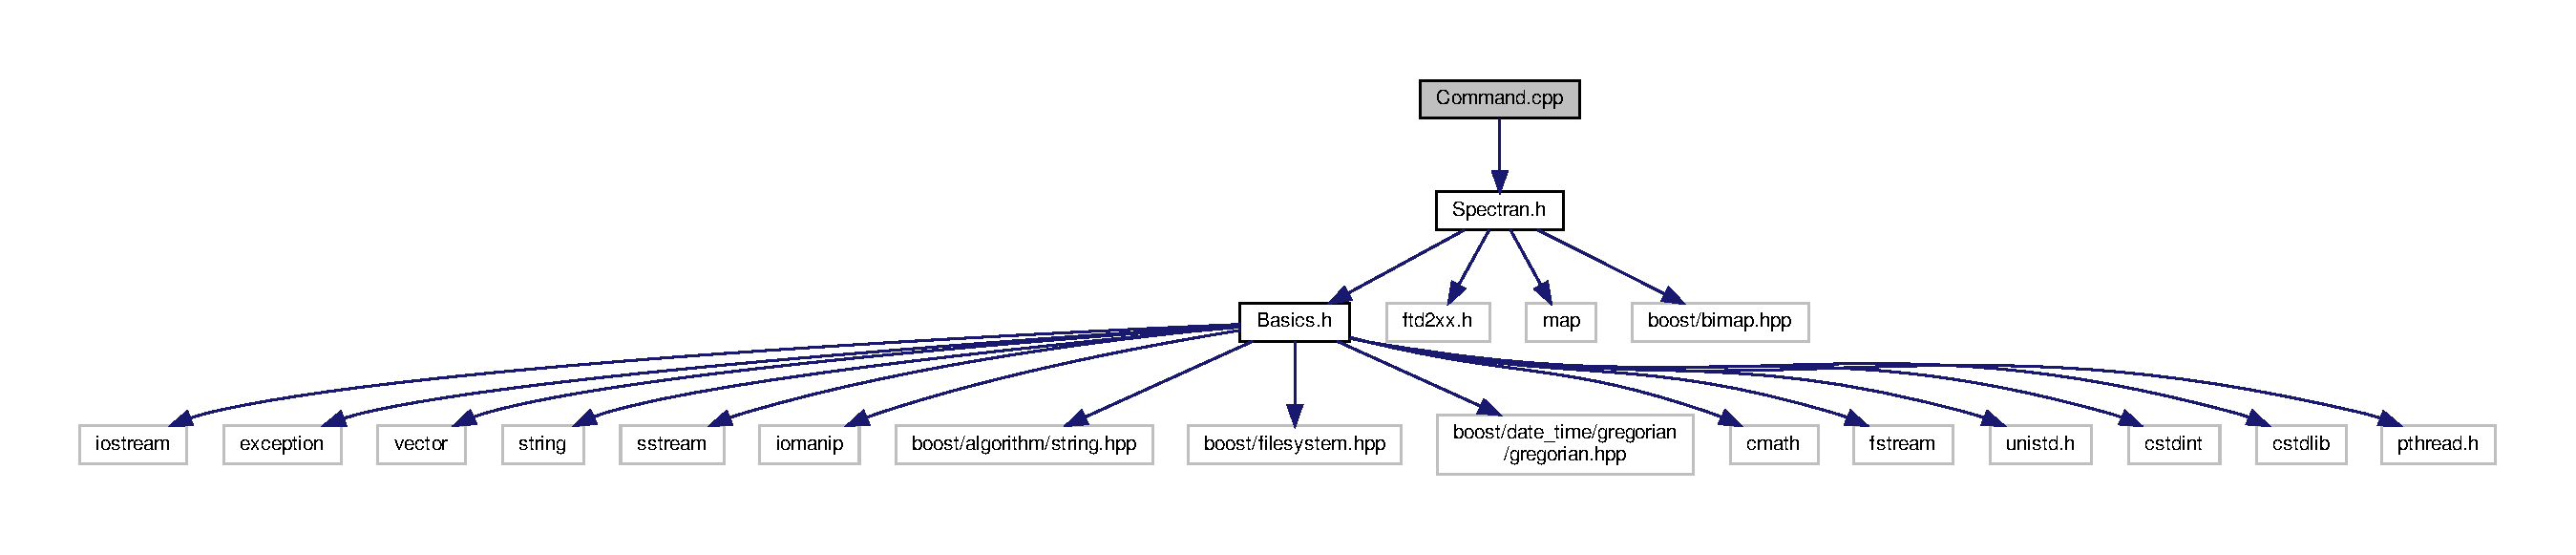
\includegraphics[width=350pt]{Command_8cpp__incl}
\end{center}
\end{figure}


\subsection{Detailed Description}
This file contains the definitions of several methods of the class {\itshape \hyperlink{classCommand}{Command}}. 

\begin{DoxyAuthor}{Author}
Mauro Diamantino 
\end{DoxyAuthor}

\hypertarget{Reply_8cpp}{}\section{/home/new-\/mauro/eclipse-\/cdt/workspace/\+R\+F\+I\+M\+S\+\_\+\+C\+A\+R\+T/src/\+Reply.cpp File Reference}
\label{Reply_8cpp}\index{/home/new-\/mauro/eclipse-\/cdt/workspace/\+R\+F\+I\+M\+S\+\_\+\+C\+A\+R\+T/src/\+Reply.\+cpp@{/home/new-\/mauro/eclipse-\/cdt/workspace/\+R\+F\+I\+M\+S\+\_\+\+C\+A\+R\+T/src/\+Reply.\+cpp}}


This file contains the definitions of several methods of the classes {\itshape \hyperlink{classReply}{Reply}} and {\itshape \hyperlink{classSweepReply}{Sweep\+Reply}}.  


{\ttfamily \#include \char`\"{}Spectran.\+h\char`\"{}}\newline
Include dependency graph for Reply.\+cpp\+:\nopagebreak
\begin{figure}[H]
\begin{center}
\leavevmode
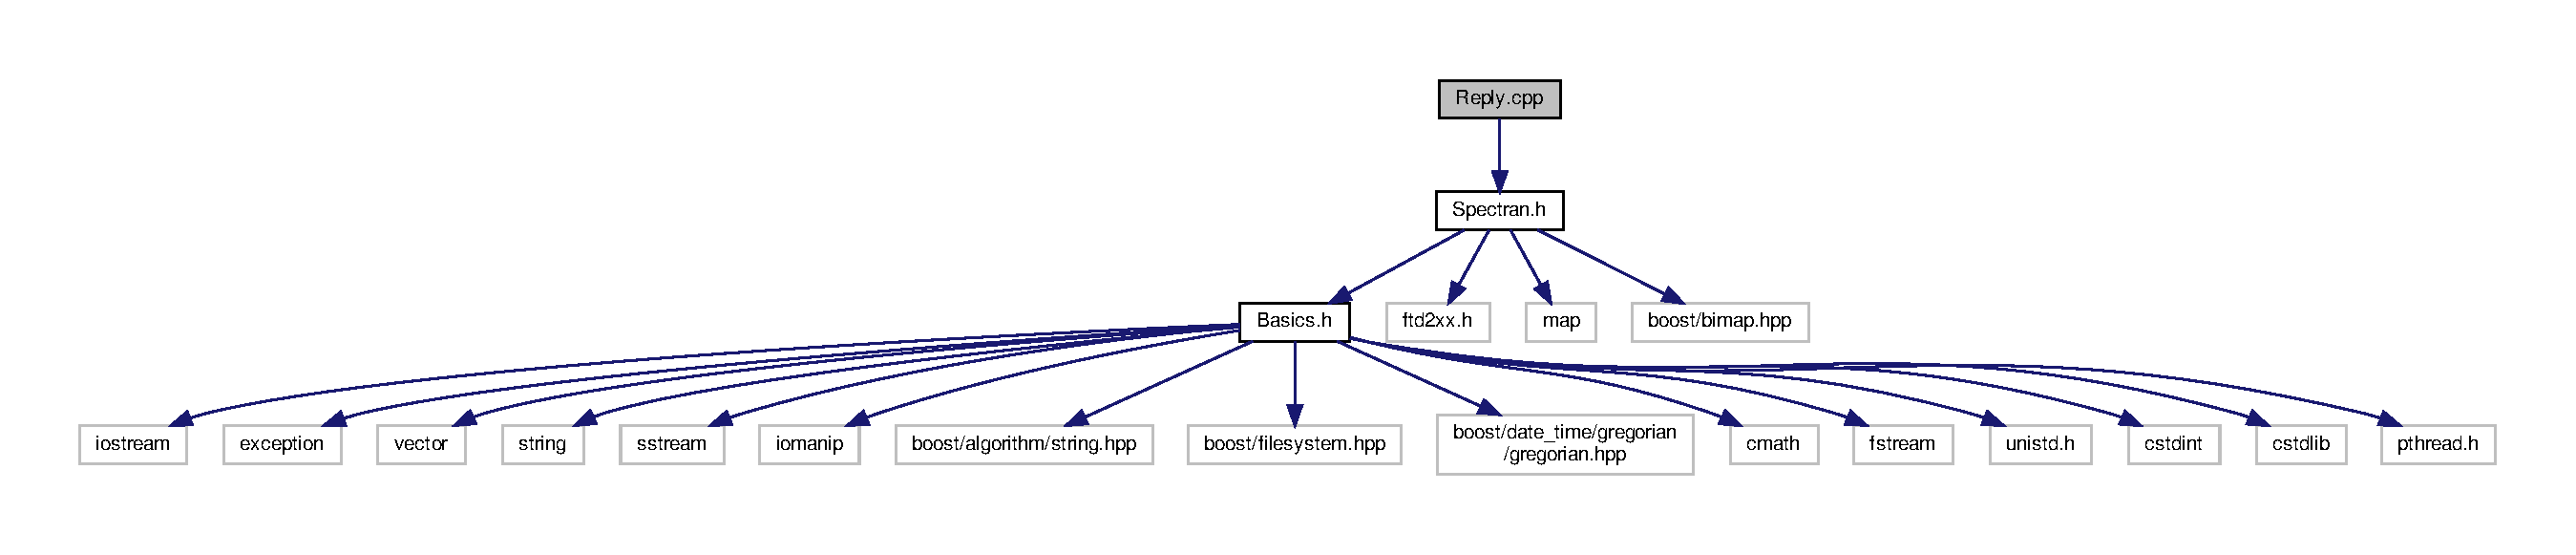
\includegraphics[width=350pt]{Reply_8cpp__incl}
\end{center}
\end{figure}


\subsection{Detailed Description}
This file contains the definitions of several methods of the classes {\itshape \hyperlink{classReply}{Reply}} and {\itshape \hyperlink{classSweepReply}{Sweep\+Reply}}. 

\begin{DoxyAuthor}{Author}
Mauro Diamantino 
\end{DoxyAuthor}

\hypertarget{Spectran_8h}{}\section{/home/new-\/mauro/eclipse-\/cdt/workspace/\+R\+F\+I\+M\+S\+\_\+\+C\+A\+R\+T/src/\+Spectran.h File Reference}
\label{Spectran_8h}\index{/home/new-\/mauro/eclipse-\/cdt/workspace/\+R\+F\+I\+M\+S\+\_\+\+C\+A\+R\+T/src/\+Spectran.\+h@{/home/new-\/mauro/eclipse-\/cdt/workspace/\+R\+F\+I\+M\+S\+\_\+\+C\+A\+R\+T/src/\+Spectran.\+h}}


This header file contains the declarations of the classes which allow the communication with the spectrum analyzer Aaronia Spectran H\+F-\/60105 V4 X.  


{\ttfamily \#include \char`\"{}Basics.\+h\char`\"{}}\newline
{\ttfamily \#include $<$ftd2xx.\+h$>$}\newline
{\ttfamily \#include $<$map$>$}\newline
{\ttfamily \#include $<$boost/bimap.\+hpp$>$}\newline
Include dependency graph for Spectran.\+h\+:\nopagebreak
\begin{figure}[H]
\begin{center}
\leavevmode
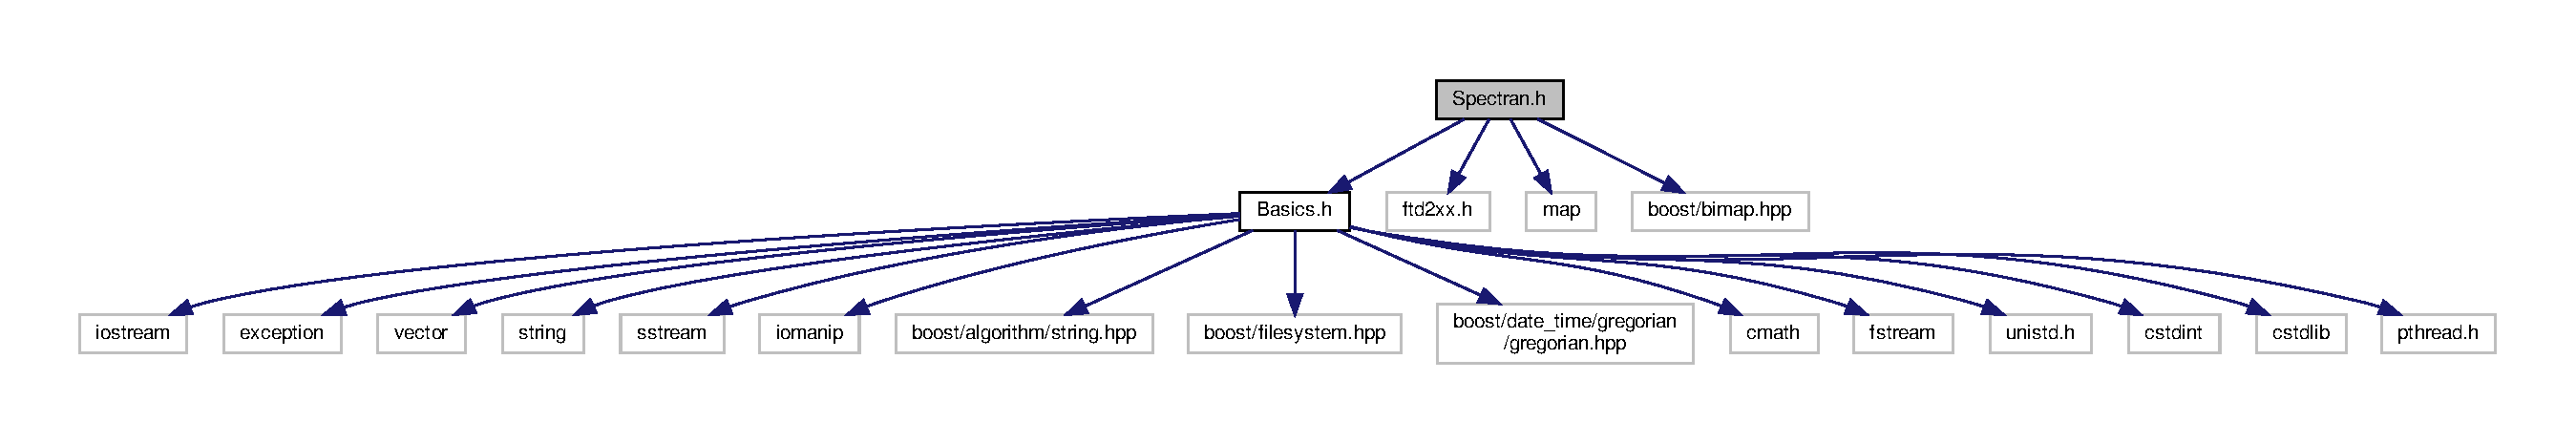
\includegraphics[width=350pt]{Spectran_8h__incl}
\end{center}
\end{figure}
This graph shows which files directly or indirectly include this file\+:\nopagebreak
\begin{figure}[H]
\begin{center}
\leavevmode
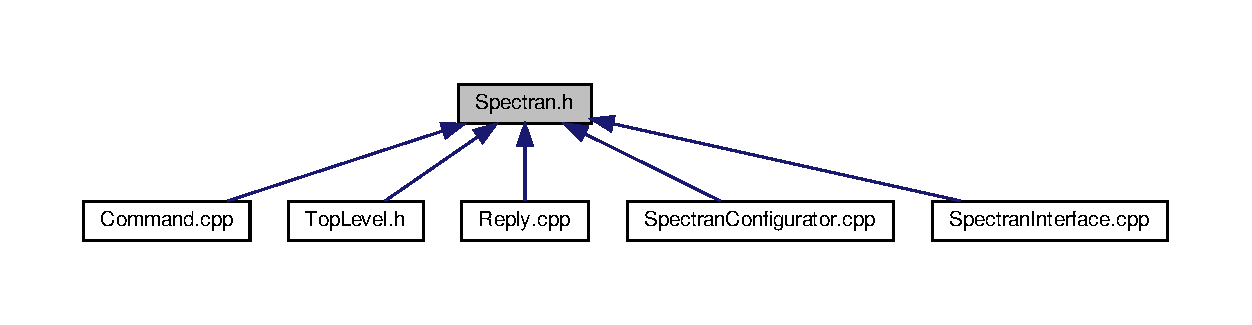
\includegraphics[width=350pt]{Spectran_8h__dep__incl}
\end{center}
\end{figure}
\subsection*{Classes}
\begin{DoxyCompactItemize}
\item 
union \hyperlink{unionFloatToBytes}{Float\+To\+Bytes}
\begin{DoxyCompactList}\small\item\em An union which is used to split a {\ttfamily float} value in its 4 bytes. \end{DoxyCompactList}\item 
class \hyperlink{classCommand}{Command}
\begin{DoxyCompactList}\small\item\em This class builds the corresponding bytes array to send a certain command to a Aaronia Spectran V4 series spectrum analyzer. \end{DoxyCompactList}\item 
class \hyperlink{classReply}{Reply}
\begin{DoxyCompactList}\small\item\em The class {\itshape \hyperlink{classReply}{Reply}} is intended to receive a bytes vector sent by the spectrum analyzer and to extract its information. \end{DoxyCompactList}\item 
class \hyperlink{classSweepReply}{Sweep\+Reply}
\begin{DoxyCompactList}\small\item\em This class derives from the base class {\itshape \hyperlink{classReply}{Reply}} and is intended to process in a better way replies with sweep points, i.\+e. {\itshape A\+M\+P\+F\+R\+E\+Q\+D\+AT} replies. \end{DoxyCompactList}\item 
class \hyperlink{classSpectranInterface}{Spectran\+Interface}
\begin{DoxyCompactList}\small\item\em The aim of this class is to manage the communication with the Aaronia Spectran device. \end{DoxyCompactList}\item 
class \hyperlink{classSpectranConfigurator}{Spectran\+Configurator}
\begin{DoxyCompactList}\small\item\em The class {\itshape \hyperlink{classSpectranConfigurator}{Spectran\+Configurator}} is intended to manage the process of configuring the Aaronia Spectran device. \end{DoxyCompactList}\item 
struct \hyperlink{structSpectranConfigurator_1_1FixedParameters}{Spectran\+Configurator\+::\+Fixed\+Parameters}
\begin{DoxyCompactList}\small\item\em This structure saves the fixed parameters of the spectrum analyzer, i.\+e. the parameters which do not change through the entire measurement cycle. \end{DoxyCompactList}\item 
class \hyperlink{classSweepBuilder}{Sweep\+Builder}
\begin{DoxyCompactList}\small\item\em The aim of class {\itshape \hyperlink{classSweepBuilder}{Sweep\+Builder}} is to build the complete sweep from the individual sweep points which are delivered by the Spectran Interface. \end{DoxyCompactList}\end{DoxyCompactItemize}
\subsection*{Typedefs}
\begin{DoxyCompactItemize}
\item 
\mbox{\Hypertarget{Spectran_8h_a39a3a5436da634ac5816e79f8a29d25c}\label{Spectran_8h_a39a3a5436da634ac5816e79f8a29d25c}} 
typedef boost\+::bimap$<$ float, float $>$ \hyperlink{Spectran_8h_a39a3a5436da634ac5816e79f8a29d25c}{R\+B\+W\+\_\+bimap}
\begin{DoxyCompactList}\small\item\em This typedef simplifies the definitions of containers of type {\ttfamily boost\+::bimap$<$float,float$>$} which is used to store R\+BW values and its indexes. \end{DoxyCompactList}\end{DoxyCompactItemize}
\subsection*{Enumerations}
\begin{DoxyCompactItemize}
\item 
enum \hyperlink{Spectran_8h_a0411392c90f0c8f0d8e44a4e94259276}{Spec\+Variable} \+: uint8\+\_\+t \{ \newline
{\bfseries S\+T\+A\+R\+T\+F\+R\+EQ} =0x01, 
{\bfseries S\+T\+O\+P\+F\+R\+EQ}, 
{\bfseries R\+E\+S\+B\+A\+N\+DW}, 
{\bfseries V\+I\+D\+B\+A\+N\+DW}, 
\newline
{\bfseries S\+W\+E\+E\+P\+T\+I\+ME}, 
{\bfseries A\+T\+T\+E\+N\+F\+AC}, 
{\bfseries R\+E\+F\+L\+E\+V\+EL}, 
{\bfseries D\+I\+S\+P\+R\+A\+N\+GE}, 
\newline
{\bfseries D\+I\+S\+P\+U\+N\+IT}, 
{\bfseries D\+E\+T\+M\+O\+DE}, 
{\bfseries D\+E\+M\+O\+D\+M\+O\+DE}, 
{\bfseries S\+P\+E\+C\+P\+R\+OC}, 
\newline
{\bfseries A\+N\+T\+T\+Y\+PE}, 
{\bfseries C\+A\+B\+L\+E\+T\+Y\+PE}, 
{\bfseries R\+E\+C\+V\+C\+O\+NF}, 
{\bfseries C\+E\+N\+T\+E\+R\+F\+R\+EQ} =0x1E, 
\newline
{\bfseries S\+P\+A\+N\+F\+R\+EQ}, 
{\bfseries P\+R\+E\+A\+M\+P\+EN} =0x10, 
{\bfseries S\+W\+P\+D\+L\+Y\+A\+CC}, 
{\bfseries S\+W\+P\+F\+R\+Q\+P\+TS}, 
\newline
{\bfseries R\+E\+F\+O\+F\+FS}, 
{\bfseries U\+S\+B\+M\+E\+AS} =0x20, 
{\bfseries U\+S\+B\+S\+W\+P\+R\+ST}, 
{\bfseries U\+S\+B\+S\+W\+P\+ID}, 
\newline
{\bfseries U\+S\+B\+R\+U\+N\+P\+R\+OG}, 
{\bfseries L\+O\+G\+F\+I\+L\+E\+ID} =0x30, 
{\bfseries L\+O\+G\+S\+A\+M\+P\+C\+NT}, 
{\bfseries L\+O\+G\+T\+I\+M\+E\+I\+VL}, 
\newline
{\bfseries S\+P\+E\+C\+D\+I\+SP} =0x41, 
{\bfseries P\+E\+A\+K\+D\+I\+SP}, 
{\bfseries M\+A\+R\+K\+M\+I\+N\+PK}, 
{\bfseries R\+D\+O\+U\+T\+I\+DX}, 
\newline
{\bfseries M\+A\+R\+K\+C\+O\+U\+NT}, 
{\bfseries L\+E\+V\+E\+L\+T\+O\+NE}, 
{\bfseries B\+A\+C\+K\+B\+B\+EN}, 
{\bfseries D\+I\+S\+P\+D\+IS}, 
\newline
{\bfseries S\+P\+K\+V\+O\+L\+U\+ME}, 
{\bfseries R\+B\+W\+F\+S\+T\+EP} =0x60, 
{\bfseries A\+N\+T\+G\+A\+IN}, 
{\bfseries P\+E\+A\+K1\+P\+OW} =0x80, 
\newline
{\bfseries P\+E\+A\+K2\+P\+OW}, 
{\bfseries P\+E\+A\+K3\+P\+OW}, 
{\bfseries P\+E\+A\+K1\+F\+R\+EQ} =0x84, 
{\bfseries P\+E\+A\+K2\+F\+R\+EQ}, 
\newline
{\bfseries P\+E\+A\+K3\+F\+R\+EQ}, 
{\bfseries M\+A\+X\+P\+E\+A\+K\+P\+OW} =0x90, 
{\bfseries S\+T\+D\+T\+O\+NE} =0x\+C0, 
{\bfseries U\+N\+I\+N\+I\+T\+I\+A\+L\+I\+Z\+ED}
 \}\begin{DoxyCompactList}\small\item\em An enumeration which contains of the names of all the environment variables of the spectrum analyzer Aaronia Spectran H\+F-\/60105 V4 X. \end{DoxyCompactList}
\end{DoxyCompactItemize}
\subsection*{Functions}
\begin{DoxyCompactItemize}
\item 
\mbox{\Hypertarget{Spectran_8h_a16fa8eb91a19fde7a399d85c521f63fd}\label{Spectran_8h_a16fa8eb91a19fde7a399d85c521f63fd}} 
const std\+::vector$<$ R\+B\+W\+\_\+bimap\+::value\+\_\+type $>$ \hyperlink{Spectran_8h_a16fa8eb91a19fde7a399d85c521f63fd}{vect} (\{ \{50e6, 0.\+0\}, \{3e6, 1.\+0\}, \{1e6, 2.\+0\}, \{300e3, 3.\+0\}, \{100e3, 4.\+0\}, \{30e3, 5.\+0\}, \{10e3, 6.\+0\}, \{3e3, 7.\+0\}, \{1e3, 8.\+0\}, \{120e3, 100.\+0\}, \{9e3, 101.\+0\}, \{200.\+0, 102.\+0\}, \{5e6, 103.\+0\}, \{200e3, 104\}, \{1.\+5e6, 105.\+0\} \})
\begin{DoxyCompactList}\small\item\em A vector which is initialized with the pairs of values \{R\+B\+W(\+Hz), R\+BW index\}. This vector is used to initialize a bidirectional map. \end{DoxyCompactList}\item 
const \hyperlink{Spectran_8h_a39a3a5436da634ac5816e79f8a29d25c}{R\+B\+W\+\_\+bimap} \hyperlink{Spectran_8h_ae551a6824a7df7b10dedc4b8743f36f5}{R\+B\+W\+\_\+\+I\+N\+D\+EX} (vect.\+begin(), vect.\+end())
\begin{DoxyCompactList}\small\item\em A bidirectional map (bimap) which contains the pairs of values \{R\+B\+W(\+Hz), R\+BW index\}. \end{DoxyCompactList}\end{DoxyCompactItemize}


\subsection{Detailed Description}
This header file contains the declarations of the classes which allow the communication with the spectrum analyzer Aaronia Spectran H\+F-\/60105 V4 X. 

The classes defined in this header file allows to set up the spectrum analyzer, read its environment variables, enable/disable the streaming of sweep points, process its responses and to capture and store the sweep points in an orderly manner. \begin{DoxyAuthor}{Author}
Mauro Diamantino 
\end{DoxyAuthor}


\subsection{Enumeration Type Documentation}
\mbox{\Hypertarget{Spectran_8h_a0411392c90f0c8f0d8e44a4e94259276}\label{Spectran_8h_a0411392c90f0c8f0d8e44a4e94259276}} 
\index{Spectran.\+h@{Spectran.\+h}!Spec\+Variable@{Spec\+Variable}}
\index{Spec\+Variable@{Spec\+Variable}!Spectran.\+h@{Spectran.\+h}}
\subsubsection{\texorpdfstring{Spec\+Variable}{SpecVariable}}
{\footnotesize\ttfamily enum \hyperlink{Spectran_8h_a0411392c90f0c8f0d8e44a4e94259276}{Spec\+Variable} \+: uint8\+\_\+t\hspace{0.3cm}{\ttfamily [strong]}}



An enumeration which contains of the names of all the environment variables of the spectrum analyzer Aaronia Spectran H\+F-\/60105 V4 X. 

Each member (a variable name) has associated an integer number which is equal to its identification index (ID), taking into account the Spectran U\+SB Protocol documentation. 

\subsection{Function Documentation}
\mbox{\Hypertarget{Spectran_8h_ae551a6824a7df7b10dedc4b8743f36f5}\label{Spectran_8h_ae551a6824a7df7b10dedc4b8743f36f5}} 
\index{Spectran.\+h@{Spectran.\+h}!R\+B\+W\+\_\+\+I\+N\+D\+EX@{R\+B\+W\+\_\+\+I\+N\+D\+EX}}
\index{R\+B\+W\+\_\+\+I\+N\+D\+EX@{R\+B\+W\+\_\+\+I\+N\+D\+EX}!Spectran.\+h@{Spectran.\+h}}
\subsubsection{\texorpdfstring{R\+B\+W\+\_\+\+I\+N\+D\+E\+X()}{RBW\_INDEX()}}
{\footnotesize\ttfamily const \hyperlink{Spectran_8h_a39a3a5436da634ac5816e79f8a29d25c}{R\+B\+W\+\_\+bimap} R\+B\+W\+\_\+\+I\+N\+D\+EX (\begin{DoxyParamCaption}\item[{vect.}]{begin(),  }\item[{vect.}]{end() }\end{DoxyParamCaption})}



A bidirectional map (bimap) which contains the pairs of values \{R\+B\+W(\+Hz), R\+BW index\}. 

These pairs of values relates a R\+BW frequency value with its corresponding index taking into account the Spectran U\+SB protocol. So this bidirectional container allows to get the corresponding index given a frequency value or to get the corresponding frequency value given an index. This allows to work with frequency values of R\+BW at high level, eliminating the need to learn the protocol\textquotesingle{}s indexes. This container is used by the classes {\itshape \hyperlink{classCommand}{Command}} and {\itshape \hyperlink{classReply}{Reply}}. 
\hypertarget{SpectranConfigurator_8cpp}{}\section{/home/new-\/mauro/eclipse-\/cdt/workspace/\+R\+F\+I\+M\+S\+\_\+\+C\+A\+R\+T/src/\+Spectran\+Configurator.cpp File Reference}
\label{SpectranConfigurator_8cpp}\index{/home/new-\/mauro/eclipse-\/cdt/workspace/\+R\+F\+I\+M\+S\+\_\+\+C\+A\+R\+T/src/\+Spectran\+Configurator.\+cpp@{/home/new-\/mauro/eclipse-\/cdt/workspace/\+R\+F\+I\+M\+S\+\_\+\+C\+A\+R\+T/src/\+Spectran\+Configurator.\+cpp}}


This file contains the definitions of several methods of the class {\itshape \hyperlink{classSpectranConfigurator}{Spectran\+Configurator}}.  


{\ttfamily \#include \char`\"{}Spectran.\+h\char`\"{}}\newline
Include dependency graph for Spectran\+Configurator.\+cpp\+:
\nopagebreak
\begin{figure}[H]
\begin{center}
\leavevmode
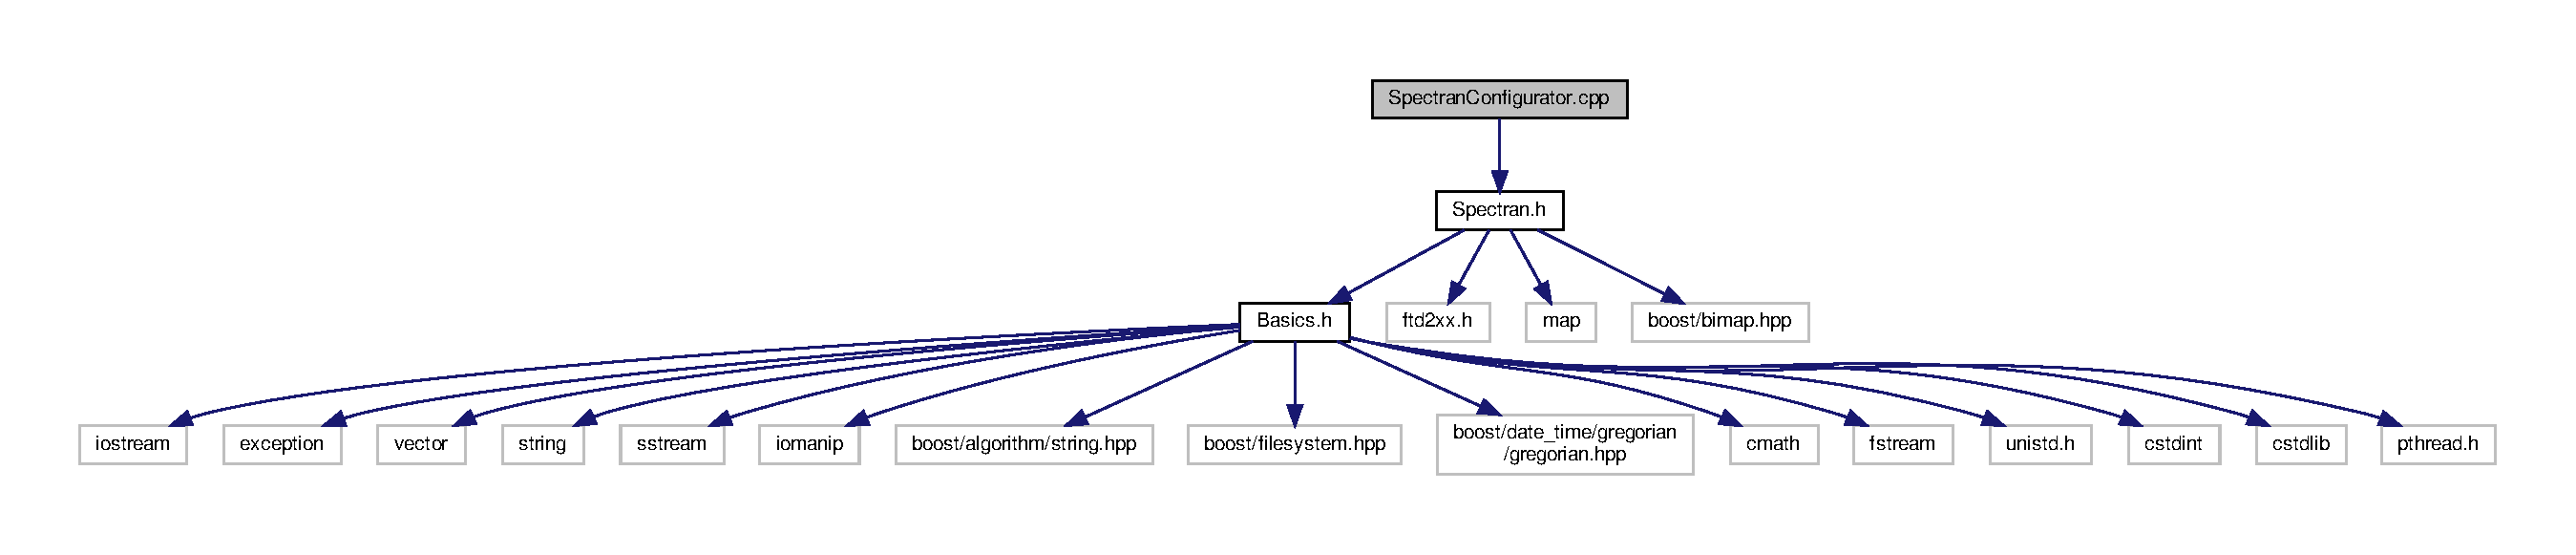
\includegraphics[width=350pt]{SpectranConfigurator_8cpp__incl}
\end{center}
\end{figure}


\subsection{Detailed Description}
This file contains the definitions of several methods of the class {\itshape \hyperlink{classSpectranConfigurator}{Spectran\+Configurator}}. 

\begin{DoxyAuthor}{Author}
Mauro Diamantino 
\end{DoxyAuthor}

\hypertarget{SpectranInterface_8cpp}{}\section{Spectran\+Interface.\+cpp File Reference}
\label{SpectranInterface_8cpp}\index{Spectran\+Interface.\+cpp@{Spectran\+Interface.\+cpp}}


This file contains the definitions of some of the methods of the class {\itshape \hyperlink{classSpectranInterface}{Spectran\+Interface}}.  


{\ttfamily \#include \char`\"{}Spectran.\+h\char`\"{}}\newline
Include dependency graph for Spectran\+Interface.\+cpp\+:\nopagebreak
\begin{figure}[H]
\begin{center}
\leavevmode
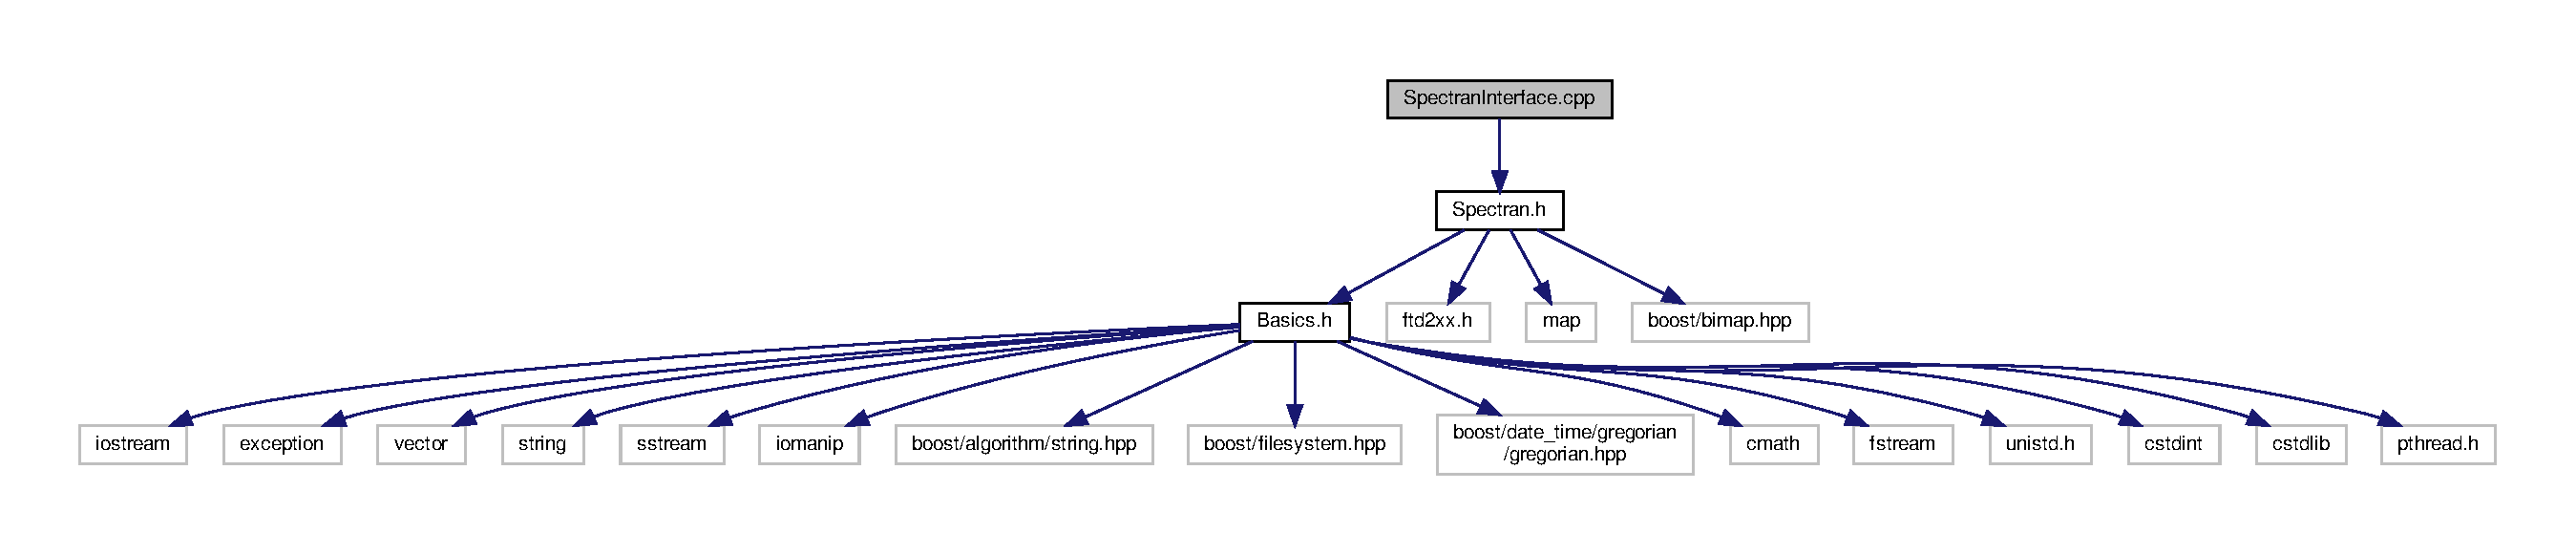
\includegraphics[width=350pt]{SpectranInterface_8cpp__incl}
\end{center}
\end{figure}


\subsection{Detailed Description}
This file contains the definitions of some of the methods of the class {\itshape \hyperlink{classSpectranInterface}{Spectran\+Interface}}. 

\begin{DoxyAuthor}{Author}
Mauro Diamantino 
\end{DoxyAuthor}

\hypertarget{SweepProcessing_8h}{}\section{/home/new-\/mauro/eclipse-\/cdt/workspace/\+R\+F\+I\+M\+S\+\_\+\+C\+A\+R\+T/src/\+Sweep\+Processing.h File Reference}
\label{SweepProcessing_8h}\index{/home/new-\/mauro/eclipse-\/cdt/workspace/\+R\+F\+I\+M\+S\+\_\+\+C\+A\+R\+T/src/\+Sweep\+Processing.\+h@{/home/new-\/mauro/eclipse-\/cdt/workspace/\+R\+F\+I\+M\+S\+\_\+\+C\+A\+R\+T/src/\+Sweep\+Processing.\+h}}


This header file contains the declarations of the classes which are responsible for the processing of each sweep, once it has been captured.  


{\ttfamily \#include \char`\"{}Basics.\+h\char`\"{}}\newline
{\ttfamily \#include \char`\"{}gnuplot\+\_\+i.\+hpp\char`\"{}}\newline
{\ttfamily \#include $<$queue$>$}\newline
Include dependency graph for Sweep\+Processing.\+h\+:
\nopagebreak
\begin{figure}[H]
\begin{center}
\leavevmode
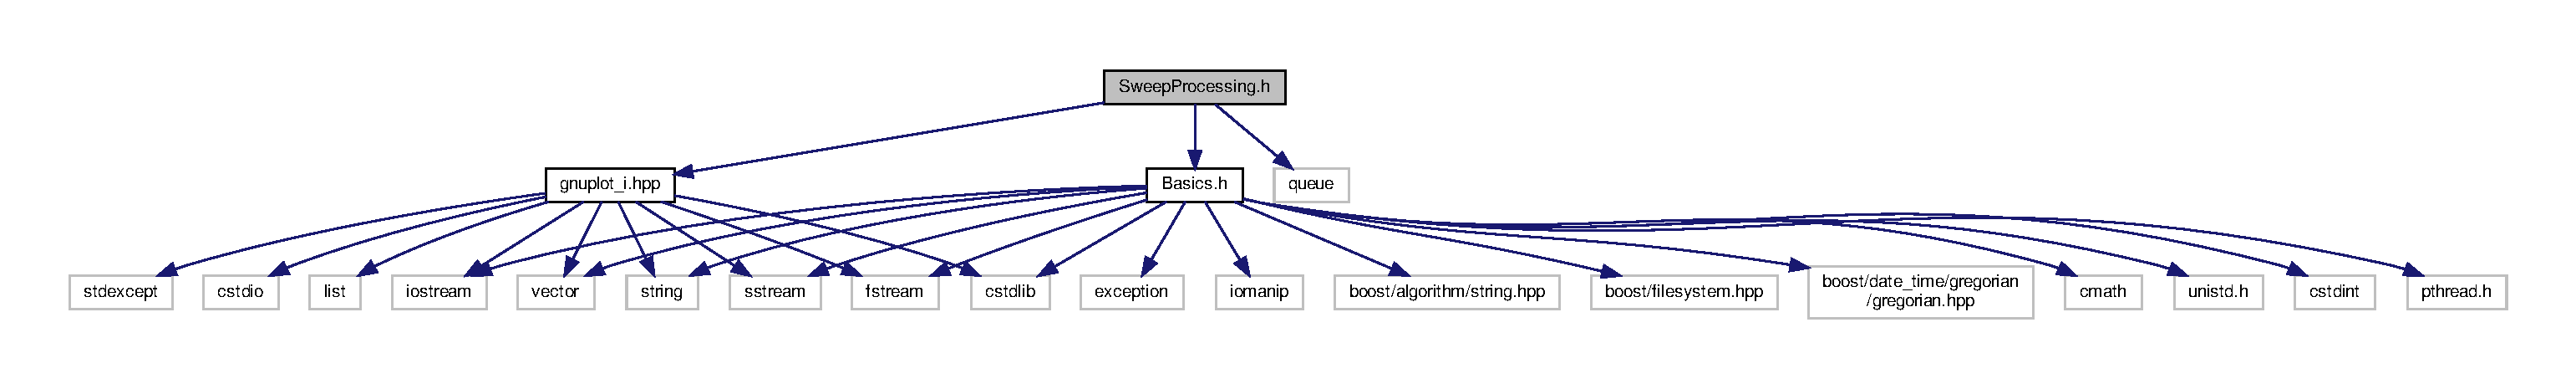
\includegraphics[width=350pt]{SweepProcessing_8h__incl}
\end{center}
\end{figure}
This graph shows which files directly or indirectly include this file\+:
\nopagebreak
\begin{figure}[H]
\begin{center}
\leavevmode
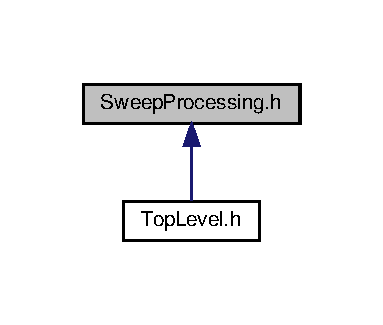
\includegraphics[width=350pt]{SweepProcessing_8h__dep__incl}
\end{center}
\end{figure}
\subsection*{Classes}
\begin{DoxyCompactItemize}
\item 
class \hyperlink{classRFPlotter}{R\+F\+Plotter}
\begin{DoxyCompactList}\small\item\em The class {\itshape \hyperlink{classRFPlotter}{R\+F\+Plotter}} is intended to plot sweeps, RF interference (\hyperlink{structRFI}{R\+FI}) and any frequency curve. \end{DoxyCompactList}\item 
class \hyperlink{classCurveAdjuster}{Curve\+Adjuster}
\begin{DoxyCompactList}\small\item\em The aim of the class {\itshape \hyperlink{classCurveAdjuster}{Curve\+Adjuster}} is to adjust any frequency curve, this is to interpolate and/or extrapolate the curve of a given parameter versus frequency. \end{DoxyCompactList}\item 
class \hyperlink{classFrontEndCalibrator}{Front\+End\+Calibrator}
\begin{DoxyCompactList}\small\item\em The aim of this class is to calculate the total gain and total noise figure curves versus frequency of the RF front end. \end{DoxyCompactList}\item 
class \hyperlink{classRFIDetector}{R\+F\+I\+Detector}
\begin{DoxyCompactList}\small\item\em The aim of this class is to compare each calibrated sweep with a threshold curve to determine where there is RF interference (\hyperlink{structRFI}{R\+FI}). \end{DoxyCompactList}\item 
class \hyperlink{classDataLogger}{Data\+Logger}
\begin{DoxyCompactList}\small\item\em The class {\itshape \hyperlink{classDataLogger}{Data\+Logger}} is intended to handle the storing of the generated data into memory, following the C\+SV (comma-\/separated values) format. \end{DoxyCompactList}\end{DoxyCompactItemize}


\subsection{Detailed Description}
This header file contains the declarations of the classes which are responsible for the processing of each sweep, once it has been captured. 

The tasks which are performed by the classes defined here are the following\+:
\begin{DoxyItemize}
\item Plotting of sweeps, \hyperlink{structRFI}{R\+FI} and any frequency curve.
\item Adjusting (interpolation) of frequency curves.
\item Front end calibration.
\item \hyperlink{structRFI}{R\+FI} detection.
\item Data logging. \begin{DoxyAuthor}{Author}
Mauro Diamantino 
\end{DoxyAuthor}

\end{DoxyItemize}
%--- End generated contents ---

% Index
\backmatter
\newpage
\phantomsection
\clearemptydoublepage
\addcontentsline{toc}{chapter}{Index}
\printindex

\end{document}
